\RequirePackage{tikz} %solve the confilict with package graphicx 
%package tikz contains package graphicx
%we need package tikz for package todonotes

\documentclass[
alternativefont, %Use WUP default font Charter and 0.9Helvetica
%nofrontmatter, %does not print the front matter pages 
%nohalftitle, %a page with halftitle at the very beginning
%notitle, %does not print the title page
%noimprint, %the page with advisor, ISBN, and so on
%acknowledgments, %prints the acknowledgments page
%nopreface, %print the preface
abstract, %prints the abstract page
abstractGerman, %prints the German abstract page
headline, %the line at the top of each page
%dedication, %prints the dedication page
%notableofcontents, %does not print the table of contents page
%nographic %avoid the conflict between packages graphicx and tikz
]{wup_v1_2}


%%%%%%%%%%%%%%%%%%%%%%%%%%%%%%%%%%%%%%
%%%%%%%%%%%%%%%%%%%%%%%%%%%%%%%%%%%%%%
%FINAL VERSION:
%look for numbered but unlabelled equations
%\usepackage{refcheck}%compile twice in order to see the effects

%To avoid warnings
%e.g., Font shape `OT1/cmr/bx/n' in size <10.5> not available(Font) size <10.95> substituted
%https://tex.stackexchange.com/questions/58087/how-to-remove-the-warnings-font-shape-ot1-cmss-m-n-in-size-4-not-available
\usepackage{anyfontsize}

%change the font sizes
%http://mirror.hmc.edu/ctan/macros/latex/base/classes.pdf, from page 7
\makeatletter
\renewcommand\normalsize{\@setfontsize\normalsize{10.5}{12.5}} %original: 10, 12
\renewcommand\small{\@setfontsize\small{9.5}{11.5}} %original: 9, 11
\renewcommand\footnotesize{\@setfontsize\footnotesize{8.5}{10}} %original: 8, 9.5
\renewcommand\scriptsize{\@setfontsize\scriptsize{7.5}{8.5}} %original: 7, 8
%I define a new fontsize the same as I used inside figures.
\newcommand\mysubcaptionfont{\@setfontsize\mysubcaptionfont\@xpt\@xiipt}
%\newcommand\mysubcaptionfont{\@setfontsize\mysubcaptionfont\@xivpt\@xivpt}
\makeatother
\small
\normalsize
\footnotesize
\scriptsize
\mysubcaptionfont

\DeclareCaptionFont{mysubcaptionfont}{\mysubcaptionfont}
%\usepackage{caption} %was defined in wup.cls
\captionsetup{
    justification=justified %Distribute text evenly between margins
}
\captionsetup[sub]{
	justification=centering,
	font=mysubcaptionfont, %I used 10pt when I drew figures
	labelformat=empty,
}




\usepackage[utf8]{inputenc}
\usepackage[T1]{fontenc}

% running footnotes in whole document 
\usepackage{chngcntr} 
\counterwithout{footnote}{chapter} 
% style of footnotes left-justified in justification 
\usepackage[bottom,hang,marginal]{footmisc} 
\setlength{\footnotemargin}{1.3em}
%extra penalty for breaking after first line of a paragraph: 
\clubpenalty = 10000 
%extra penalty for breaking before last line of a paragraph:
\widowpenalty = 10000
%extra penalty for breaking before last line before a display math:
\displaywidowpenalty = 10000

\graphicspath{{images/}}
\usepackage{wrapfig}
%\usepackage[ngerman]{babel}
\usepackage[english]{babel} % to write documents in languages


\usepackage{lipsum}  % Loading lipsum to write blind text


\usepackage{amsmath}  %align equations; text inside math

\usepackage{amsthm} %for using open problem
\theoremstyle{definition}
\newtheorem{open}{Open Problem}

%\usepackage{array}%for making new column types; included
\usepackage{bm} %make a variable bold in math mode 
\usepackage{booktabs} %for using \toprule, \midrule, and 
%\bottomrule in a table
\usepackage{dcolumn} %for \newcolumntype{d}[1]{D{'}{.}{#1}}
%https://stackoverflow.com/questions/4968557/latex-very-compact-itemize/4974583#4974583
\usepackage{enumitem} %for compact itemize
\usepackage{float} %option "H" for placing a figure
\usepackage[bottom]{footmisc}% places footnotes at page bottom
\usepackage{gensymb}  % for degree sign
% when including figure files
\usepackage[defaultlines=4,all]{nowidow}%forbid widow or orphan

\usepackage{ragged2e}
\justifying

\usepackage{hyperref}
\hypersetup{linktocpage=true}
\hypersetup{colorlinks=true}
\hypersetup{hidelinks}
%\hypersetup{pdftitle = {An Optimization-Based Approach for 
%		Continuous Map Generalization}}
\hypersetup{pdfauthor = {Dongliang Peng}}
\hypersetup{pdfsubject = {Dissertation}}
\hypersetup{pdfkeywords = {Land-cover area, Administrative boundary, 
Building, Morphing, Data structure, Zooming}}
\hypersetup{pdfdisplaydoctitle = true}
\newcommand{\dlpLinkColor}{black}
\hypersetup{
	linktoc=all,
	colorlinks,
	citecolor=\dlpLinkColor,
	filecolor=\dlpLinkColor,
	linkcolor=black,
	urlcolor=\dlpLinkColor
}

%prevent links in bibliography overflowing into the margin
%https://tex.stackexchange.com/questions/115690/urls-in-bibliography-latex-not-breaking-line-as-expected
%\hypersetup{breaklinks=true}
\usepackage{url}
\urlstyle{same}
%\Urlmuskip=0mu plus 1mu\relax

%make the font of math charter; for \mathbb
%cal=cmcal: make a difference between $\mathcal{H}$ and $\mathscr{H}$
%see https://tex.stackexchange.com/questions/454415/how-to-use-mathcal-fonts-with-charter-font-from-mathdesign
\usepackage[charter,cal=cmcal]{mathdesign}


\usepackage{multicol}        % used for the two-column index
%\pgfplotsset{compat=1.3} %make the label tight in axis picture

%\usepackage{sansmathfonts}%make the font in math model sansserif
\usepackage{tabularx} %to define the style of a column in a table


%To encourage LaTeX not to move your figure, 
%you may need to loosen its demands.
%https://texfaq.org/FAQ-floats
\renewcommand{\textfraction}{0.01}
\renewcommand{\topfraction}{0.99}
\renewcommand{\bottomfraction}{0.99}
\renewcommand{\dbltopfraction}{0.99} % fit big float above 
%\renewcommand{\topfraction}{.85}
%\renewcommand{\bottomfraction}{.7}
%\renewcommand{\textfraction}{.15}
\renewcommand{\floatpagefraction}{.66}
%\renewcommand{\dbltopfraction}{.66}
\renewcommand{\dblfloatpagefraction}{.66}
\setcounter{topnumber}{9}
\setcounter{bottomnumber}{9}
\setcounter{totalnumber}{20}
\setcounter{dbltopnumber}{9}


\usepackage[disable]{todonotes} %need package tikz
%\usepackage[textwidth=2cm]{todonotes}
\makeatletter %make package todonotes compatible with wup.cls 
\providecommand\@dotsep{5}
\renewcommand{\listoftodos}[1][\@todonotes@todolistname]{%
	\@starttoc{tdo}{#1}}
\makeatother

\usepackage{xspace} %we use \xspace for \Astar

%if a figure is on an empty last page,
%the figure will be placed at the top instead in the middle of 
%the page
\makeatletter
\setlength{\@fptop}{0pt}
\setlength{\@fpsep}{8pt} %8pt between two figures at last page
\makeatother



%style: Loads bibliography style .bbx and citation style cbx
%bibstyle: Loads bibliography style .bbx
\usepackage[
backend=biber,
%backend=bibtex,
%style=trad-alpha,
style=alphabetic, %style for my thesis
sorting=nyt, %sort by name, year, title
%bibstyle=authoryear, %no indices before names; year after names
%bibstyle=numeric, %number the references
hyperref=true,%transform citations and back references into 
%clickable hyperlinks
backref=true, %to print back references in the bibliography
backrefstyle=three, %Compress three or more consecutive pages 
%to a range
%,
%citestyle=authoryear,
maxbibnames=9, %the author names appearing in bibliography
maxcitenames=2, %the author names appearing in text
giveninits=true,
%terseinits=true,%remove periods after initials of first names
%doi=false,
%isbn=false,url=false,
eprint=false,
%dashed=false,
useprefix=false,%sort bibliography not using prefix like "van"
natbib=true]{biblatex}
\addbibresource{general/Reference/BibReference.bib}

\DeclareNameAlias{author}{family-given}%lastname before firstname
%\renewcommand*{\revsdnamepunct}{} %remove commas between last 
%and first names






%if a reference has doi, then we print only doi in bibliography;
%otherwise, we print only url
%we don't use eprint
%we must deactivate eprint by using "eprint=false"
\renewbibmacro*{doi+eprint+url}{% 
	\iftoggle{bbx:url} 
	{\iffieldundef{doi}{\usebibmacro{url+urldate}}{}} 
	{}% 
	%	\newunit\newblock 
	%	\iftoggle{bbx:eprint} 
	%	{\usebibmacro{eprint}} 
	%	{}% 
	\newunit\newblock 
	\iftoggle{bbx:doi} 
	{\printfield{doi}} 
	{}}	



%remove the information we don't want to present
\AtEveryBibitem{% Clean up the bibtex rather than editing it
	\clearlist{address}
	\clearfield{date}
%	\clearfield{eprint}
	\clearfield{isbn}
	\clearfield{issn}
	\clearlist{location}
	\clearfield{month}
	\clearlist{language}
	%	\clearfield{series}
	
	\ifentrytype{book}{}{% Remove publisher and editor except for books
		\clearlist{publisher}
		%		\clearname{editor}
	}
}

%%display pagetotal of proceedings
%\DeclareFieldFormat[inproceedings]{pagetotal}{\mkpagetotal[bookpagination]{#1}}
%\renewbibmacro*{chapter+pages}{%
%	\printfield{note}%
%	\setunit{\bibpagespunct}%
%	\printfield{pages}%
%	\setunit{\bibpagespunct}%
%	\printfield{pagetotal}%
%	\newunit}

%\ppspace defaults to \addnbspace, a non-breaking space
%we redefine \ppspace to a normal space
%https://tex.stackexchange.com/questions/167065/what-is-the-reason-to-put-a-tilde-between-p-page-and-the-number
\renewcommand{\ppspace}{ }
%change "cited on page(s)" to "see page(s)" in Bibliography
\DefineBibliographyStrings{english}{
  backrefpage  = {see p\adddot},
  backrefpages = {see pp\adddot},
  %https://tex.stackexchange.com/questions/277272/biblatex-how-to-remove-the-period-after-p-pp-in-bibliography-only
%  page  = {p\adddot},
%  pages = {pp\adddot},
}

%change parentheses of backrefs to brackets in Bibliography
\renewbibmacro*{pageref}{%
  \iflistundef{pageref}
    {}
    {\printtext[brackets]{%\printtext[parens]
       \ifnumgreater{\value{pageref}}{1}
         {\bibstring{backrefpages}\ppspace}
         {\bibstring{backrefpage}\ppspace}%
       \printlist[pageref][-\value{listtotal}]{pageref}}}}





%\iffalse
%For the references, the following commands make the titles 
%lowercase (sentence case),
%while keep book/journal/conference etc. names unchanged 
\DeclareFieldFormat{sentencecase}{\MakeSentenceCase{#1}}
\renewbibmacro*{title}{%
	\ifthenelse{\iffieldundef{title}\AND\iffieldundef{subtitle}}
	{}
	{\ifthenelse{\ifentrytype{article}\OR\ifentrytype{inbook}%
			\OR\ifentrytype{incollection}\OR\ifentrytype{inproceedings}%
			\OR\ifentrytype{inreference}}
		{\printtext[title]{%
				\printfield[sentencecase]{title}%
				\setunit{\subtitlepunct}%
				\printfield[sentencecase]{subtitle}}}%
		{\printtext[title]{%
				\printfield[titlecase]{title}%
				\setunit{\subtitlepunct}%
				\printfield[titlecase]{subtitle}}}%
		\newunit}%
	\printfield{titleaddon}}

%Remove the quotation marks for the titles in the reference
\DeclareFieldFormat[article,inbook,incollection,inproceedings,
patent,thesis,unpublished]{citetitle}{#1}
\DeclareFieldFormat[article,inbook,incollection,inproceedings,
patent,thesis,unpublished]{title}{#1}



%make the prefix of a name capital, e.g., van Dijk -> Van Dijk
%https://tex.stackexchange.com/questions/226893/biblatex-handling-of-dutch-van-prefix
\renewbibmacro*{begentry}{\midsentence} %lower-case in the bibliography
\makeatletter
\AtBeginDocument{\toggletrue{blx@useprefix}}
\makeatother

%change \textsc{DOI} to DOI, and so on, in bibliography
%https://tex.stackexchange.com/questions/58636/how-to-change-the-font-for-biblatex-acronyms
\renewcommand*{\mkbibacro}[1]{#1}

%General


\newcommand{\revise}[2]{#2}
\newcommand{\mypar}[1]{\bigskip\noindent\textbf{#1.}~}
%\newcommand{\mysmalltitle}[1]{{\bigskip\noindent\sffamily\bfseries #1}}

%define that formats for subsubsections
\titleformat{\subsubsection}
{\normalfont\sffamily\bfseries}{\thesubsubsection}{1em}{}


\newcommand{\AreaAggTitle}
%{Finding Optimal Sequences for Area 
%Aggregation---\Astar vs.\ Integer Linear Programming}
{Finding Optimal Sequences
 \\ for Area Aggregation---
 \\ \Astar vs.\ Integer Linear Programming}
\newcommand{\AreaAggToCTitle}
{Finding Optimal Sequences for Area 
Aggregation---\texorpdfstring{\Astar vs.\ Integer Linear Programming}
                             {A* vs.\ Integer Linear Programming}}
\newcommand{\AreaAggChapterMark}
{Finding Optimal Sequences for Area Aggregation}

\newcommand{\AdminBoundTitle}
%{Continuously Generalizing Administrative Boundaries Based on Compatible Triangulations}
{Continuously Generalizing\\ 
 Administrative Boundaries\\
 Based on Compatible Triangulations}
\newcommand{\AdminBoundToCTitle}
{Continuously Generalizing Administrative Boundaries
 Based on Compatible Triangulations}     
\newcommand{\AdminBoundChapterMark}
{Continuously Generalizing Administrative Boundaries Based on CTs}

\newcommand{\BldgGrowTitle}
%{Continuously Generalizing Buildings to Built-up Areas
% by Aggregating and Growing}
{Continuously Generalizing\\ 
   	Buildings to Built-up Areas\\
   	by Aggregating and Growing}
\newcommand{\BldgGrowToCTitle}
{Continuously Generalizing Buildings to Built-up Areas
 by Aggregating and Growing}
\newcommand{\BldgGrowChapterMark}
{Continuously Generalizing Buildings to Built-up Areas}

\newcommand{\MorphTitle}
%{Morphing Polylines Based on Least-Squares Adjustment}
{Morphing Polylines\\
 Based on Least-Squares Adjustment}
\newcommand{\MorphToCTitle}
{Morphing Polylines Based on Least-Squares Adjustment}

\newcommand{\DataStrTitle}
%{Choosing the Right Data Structures for Solving Spatial Problems}
{Choosing the Right Data Structures\\
 for Solving Spatial Problems}
\newcommand{\DataStrToCTitle}
{Choosing the Right Data Structures for Solving Spatial Problems}

%Preface: Adminstrative Boundaries
\newcommand{\ml}{\ensuremath{M_+}\xspace}
\newcommand{\ms}{\ensuremath{M_-}\xspace}
%\newcommand*{\mine}[1]{{\color{red}#1}}
\newcommand*{\mine}[1]{{#1}}

%see https://tex.stackexchange.com/questions/7032/good-way-to-make-textcircled-numbers
\newcommand{\circled}[1]{\textcircled{#1}}


% math-mode version of "l" column type
\newcolumntype{L}{>{$}l<{$}}
% math-mode version of "r" column type
\newcolumntype{R}{>{$}r<{$}}
% math-mode version of "c" column type
\newcolumntype{C}{>{$}c<{$}}
%align numbers by decimal points in table; 
%need package {dcolumn} and {array}
%see http://www.ctex.org/documents/packages/table/dcolumn.pdf 
\newcolumntype{d}[1]{D{'}{.}{#1}}
\newcolumntype{s}[1]{D{'}{~}{#1}}

%x:l, y:c, z:r, with specified width
%place text in a cell at top (b), middle (m), or bottom (p)
\newcolumntype{x}[1]
{>{\raggedright\arraybackslash\hspace{0pt}}m{#1}}
\newcolumntype{y}[1]
{>{\centering\arraybackslash\hspace{0pt}}m{#1}}
\newcolumntype{z}[1]
{>{\raggedleft\arraybackslash\hspace{0pt}}m{#1}}

%%math-mode version of "x,y,z" column type
%\newcolumntype{X}[1]
%{>{\raggedright\arraybackslash\hspace{0pt}}m{$#1$}}
%\newcolumntype{Y}[1]
%{>{\centering\arraybackslash\hspace{0pt}}m{$#1$}}
%\newcolumntype{Z}[1]
%{>{\raggedleft\arraybackslash\hspace{0pt}}m{$#1$}}

\newcommand{\dtrm}[2][]{d_{\mathrm{#2}, 
t\ifthenelse{\equal{#1}{}}{}{_#1}}}

%%Area Aggregation
%%**************************************************************
\newcommand{\Astar}{A$^{\!\star}$\xspace}
\newcommand{\AstarTwo}{A$^{\!\star}_{\,200{,}000}$\xspace}
\newcommand{\AstarFour}{A$^{\!\star}_{\,400{,}000}$\xspace}
\newcommand{\ILPOne}{ILP$_{100\,\mathrm{s}}$\xspace}
\newcommand{\ILPTwo}{ILP$_{200\,\mathrm{s}}$\xspace}

\newcommand{\tstar}{\ensuremath{t\xspace}}
\newcommand{\Pistar}{\ensuremath{\Pi}} % 
%\newcommand{\Comp}[1]{c_#1} % 
\newcommand{\comp}[1]{[#1]} % 
\newcommand{\edgenum}[1]{\|#1\|}
\newcommand{\area}[1]{\overline{#1}}
%{\Pi_{\mathrm{start}}(\tstar)}
\newcommand{\Pstart}{\ensuremath{P_\mathrm{start}}\xspace}
\newcommand{\Pgoal}{\ensuremath{P_\mathrm{goal}}\xspace}
\newcommand{\Pnode}{\ensuremath{P_{t,i}}\xspace}
\newcommand{\Psnode}{\ensuremath{P_{s,i}}\xspace}
\newcommand{\Tgoal}{\ensuremath{T_\mathrm{goal}}\xspace}


\newcommand{\e}[1]{\times 10^{#1}}
\newcommand{\fig}{Figure~}
\newcommand{\eq}{Equation~}
\newcommand{\fo}{Formula~}
\newcommand{\sect}{Section~}
\newcommand{\tab}{Table~}
\newcommand{\chap}{Chapter~}
\newcommand{\figs}{Figures~}
\newcommand{\eqs}{Equations~}
\newcommand{\fos}{Formulas~}
\newcommand{\sects}{Sections~}
\newcommand{\tabs}{Tables~}
\newcommand{\chaps}{Chapters~}
\newcommand{\myquad}[1][1]{\hspace*{#1em}\ignorespaces}
\newcommand{\eqquadVariable}{\myquad[6]}
\newcommand{\eqquadCost}{\myquad[2]}
\newcommand{\eqquadConstraintsX}{\myquad[4]}
\newcommand{\eqquadConstraintsYZ}{\myquad[3]}
\newcommand{\eqquadConstraintsC}{\myquad[3]}
\newcommand{\eqquadConstraints}{\myquad[3]}
\newcommand{\eqquadConstraintW}{\myquad[3]}
\newcommand{\inquad}{\qquad}
\newcommand{\inquadC}{\myquad[1]}

%because of \begin{array}
%\newcommand{\embshift}{\hspace{0.5pt}}%for tsas 
%\newcommand{\embshift}{\hspace{-3pt}}%for my thesis(10pt)
\newcommand{\embshift}{\hspace{-2.7pt}}%for my thesis(10.5pt)

%M or N are default tags. 
%The boxes using the same tag will have the same length. 
%The length is the maximum length of all the equations 
%in the boxes that use the same tag; see also 
%https://tex.stackexchange.com/questions/381502/how-to-align-text-in-multiple-separate-align-environments
\usepackage{eqparbox}
\newcommand{\embl}[2][M]
{\eqmakebox[#1][l]{$#2$}}
\newcommand{\embr}[2][N]
{\eqmakebox[#1][r]{$#2$}}
\newcommand{\embld}[2][M]
{\eqmakebox[#1][l]{$\displaystyle#2$}}
\newcommand{\embrd}[2][N]
{\eqmakebox[#1][r]{$\displaystyle#2$}}

%avoid warning
%https://tex.stackexchange.com/questions/229638/package-biblatex-warning-babel-polyglossia-detected-but-csquotes-missing
\usepackage{csquotes}

%to avoid many conflicts
%e.g., "Warning: Command \textcircled invalid in math mode"
%e.g., "Warning: Not defining \perthousand."
%e.g., "Warning: Font shape `OMS/cmsy/b/n' in size <3.75> not available(Font) size <5> substituted"
%https://tex.stackexchange.com/questions/139241/using-matbbz-and-textregistered-in-math-mode
\usepackage{textcomp}

%define command \blankpage
%https://tex.stackexchange.com/questions/36880/insert-a-blank-page-after-current-page
\def\blankpage{%
      \clearpage%
      \thispagestyle{empty}%
      \addtocounter{page}{-1}%
      \null%
      \clearpage}

%make package refcheck compatible with package hyperref 
\makeatletter
\AtBeginDocument{%
	\@ifpackageloaded{refcheck}{%
		\@ifundefined{hyperref}{}{%
			\let\T@ref@orig\T@ref
			\def\T@ref#1{\T@ref@orig{#1}\wrtusdrf{#1}}%
			\let\@refstar@orig\@refstar
			\def\@refstar#1{\@refstar@orig{#1}\wrtusdrf{#1}}%
			\DeclareRobustCommand\ref{\@ifstar\@refstar\T@ref}%
		}%
	}{}%
}
\makeatother
%-------------------
% WUP class commands
%-------------------

\TitleHalf{An Optimization-Based Approach \\ 
	for Continuous Map Generalization %\\ (manuscript, \today)
}
\Title{An Optimization-Based Approach \\ 
	for Continuous Map Generalization}
\SubTitle{}
\Author{Dongliang Peng}

\Faculty{Fakult\"at f\"ur Mathematik und Informatik}
%\Faculty{Faculty of Mathematics and Computer Science}
\YearSubmission{2017}
\YearPublication{2019}
\Advisor{Prof.\ Dr.\ Alexander Wolff and Prof.\ Dr.\ Dirk Burghardt}
\FreeTextImprint{
%\\
%\setlength{\tabcolsep}{0em}	
%\begin{tabular}{x{2.5cm}l}
%Supervisors:	    & ~Prof.\ Dr.\ Alexander Wolff\\
%					& ~Prof.\ Dr.\ Jan-Henrik Haunert
%					\vspace{4pt}\\ 
%Reviewers:			& ~Prof.\ Dr.\ Alexander Wolff\\
%					& ~Prof.\ Dr.\ Dirk Burghardt
%					\vspace{4pt}\\
%Defense Examiners:	& ~Prof.\ Dr.\ Andreas N\"uchter\\
%					& ~Prof.\ Dr.\ Jan-Henrik Haunert\\
%					& ~Prof.\ Dr.\ Alexander Wolff
%					\vspace{4pt}\\
%\multicolumn{2}{l}{Defended on December 21, 2017}					
%\end{tabular}
}
%\Edition{2nd edition}


\CoverDesign{Jule Petzold}
%\FreeTextDesign{a free text for design}

\ISBNprint{978-3-95826-104-4}
\ISBNonline{978-3-95826-105-1}
\DOI{10.25972/wup-978-3-95826-105-1}
\URN{urn:nbn:de:bvb:20-opus-174427}

\Dedication{%
the dedication
}
\Acknowledgments{%
}


\Preface{%

In his thesis, Dongliang Peng investigates computational aspects of
a fundamental problem in cartography called \emph{generalization}.
Cartographic generalization is~the~prob-lem that has to be solved
when producing a small-scale map (say, at scale $1:10{,}000$) from data
collected at a larger scale (say, $1:2{,}000$).  Traditionally, this
has been a labor-intensive task that required highly-skilled
cartographers with expertise in both geodesy and map-making.  How
should a row of ten houses be represented if the distances between
them are too small to be represented correctly at the desired scale?
By fewer, say, five houses?  Or rather by a block of houses?

Dongliang attacks this and several other special cases of
cartographic generalization in a modern setting.  Think of online
maps that users can (and want to!) zoom and pan with their finger
tips.  Other than traditional paper maps that were produced and
printed for a fixed, small number of scales, online maps should
ideally be available at \emph{any} scale (within a reasonable
interval).  The problem of computing and displaying maps at
arbitrary scales is called \emph{continuous generalization}.  Some
aspects of continuous generalization (such as the example with the
houses above) are inherently discrete, others (such as a wiggly
river) can be treated more easily in a continuous fashion.

In several chapters of this thesis, Dongliang approaches continuous
generalization problems in an innovative, yet formal way by using
powerful tools from mathematical optimization such as integer linear
programming.  The main advantage of such an approach is that it
helps to get the \emph{model} right.  Many problems can be cast into
integer linear programs, which allows us to solve at least small
examples to optimality---according to our model.  If these
solutions don't turn out as expected, we know that 
%our problem formulation, 
our model is wrong---not the algorithm.  In contrast,
when using only heuristics, solutions can come with errors of two
types; those caused by the heuristic and those caused by the model.
In this case, it is hard to understand and fix the errors.

In Chapter~2, Dongliang compares two potentially exact methods for
the well-known area-aggregation problem.  He asks for an optimal
sequence of operations that aggregates, step-by-step, many
``patches'' of a detailed map into a single region of a coarser map.
Dongliang uses a graph-based model in which he finds shortest paths
(aka optimal aggregation sequences) using the \Astar algorithm
and integer linear programming. The latter turns out to be much slower.
He also compares the \Astar algorithm to an obvious greedy
approach, which is surprisingly good given its simplicity.  He also
identifies a problem with his model.

Chapter~3 treats a related problem: how to best transit between
two levels of administrative boundaries for zooming?  The
input consists of the two drawings at start and target scale, and
the task is to mediate between the two in a continuous and
topologically safe way. 
%that is, without introducing
%self-intersections or other degeneracies.  
Dongliang finds the first
topologically safe method of solving this problem based on
\emph{compatible triangulations} (a tool from computational
geometry).  Unfortunately, the existing algorithm for compatible
triangulations sometimes introduces strong distortion locally.  A
way out may consist in choosing the Steiner points for the
compatible triangulations more carefully, but this is left as an
open problem.

In Chapter~4, Dongliang deals with the generalization of buildings.
He shows how to generalize building footprints continuously such
that well-defined blocks of buildings appear when the user of a
digital map zooms out far enough.  Here, only the building
footprints are given.  The approach animates a growing-process
between the start scale and a target scale that can be set by the
user.  The algorithm computes a drawing for the target scale by a
wisely chosen sequence of dilations and erosions
(which have been used for building simplification before).  
In order to animate the
growing-process in a continuous fashion, the buildings are expanded
in a simple way: by moving their boundaries at constant speed and by
clipping any part that leaves the target footprint.  In order to
guarantee a certain minimum distance between two buildings, the
algorithm builds bridges between close-enough buildings.  
The computation of the bridges is based on 
a minimum spanning tree of the buildings.  
The resulting animations look very natural.

In Chapter~5, Dongliang explores an important subproblem that often
appears in continuous generalization: how to ``morph'' a polygonal
chain from a start to a target scale.  He uses an existing algorithm
to define a correspondence between the two chains and then computes
trajectories for each pair of corresponding vertices.  
The aim is to find trajectories such that 
the angles and the edge lengths change 
in a uniform and continuous fashion---if possible.  
Dongliang applies least-squares adjustment in order to
gradually move the chain from its start configuration to the target
chain.  While the results on real-world data look quite good,
Dongliang also found artificial examples where self-intersection and
numerical problems occur.  Hence, least squares is probably not the
ideal method for this problem.

Finally, in Chapter~6, Dongliang presents a case study to highlight
the difficulties when working with geographic data naively.  As a
concrete example, he considers the problem of finding, in a set of
$n$ points in the plane, all pairs of points that are closer to each
other than a given threshold~$\varepsilon$.  He compares three
approaches for this problem, the text-book approach based on the
sweep-line paradigm, a Delaunay-triangulation-based approach, and a
simple grid-based approach.  While the grid-based approach wins in
terms of runtime, the different implementations of the sweep-line
algorithms are what makes the comparison interesting---a lot
depends on how the library methods are implemented, 
so the programmer should always read the fine print.

In his thesis, Dongliang exemplifies the optimization-based approach
at various continuous generalization problems and demonstrates the
strength of this approach.  We see this as a very valuable
contribution to GIScience where very all too often, problems are not
modeled properly, and then algorithms are devised that happen to
produce good-looking results on a small set of benchmark instances.
We hope that many readers of this thesis will get inspired by
Dongliang's way of tackling spatial problems!

\bigskip
\bigskip


\noindent
Alexander Wolff (first supervisor)\\
Chair of Algorithms, 
Complexity and Knowledge-Based Systems\\
Faculty of Mathematics and Computer Science\\
University of W\"urzburg

\bigskip

\noindent
Jan-Henrik Haunert (second supervisor)\\
%Geoinformation Group\\
Institute of Geodesy and Geoinformation\\
Faculty of Agriculture\\
University of Bonn
}


\Abstract{	
Maps are the main tool to represent geographical information. 
Geographical information is usually scale-dependent, 
so users need to have access to maps at different scales.
In our digital age, the access is realized by zooming.
As discrete changes during the zooming tend to distract users,
smooth changes are preferred.
This is why some digital maps 
are trying to make the zooming as continuous as they can.
The process of producing maps at different scales
with smooth changes 
is called \emph{continuous map generalization}.

In order to produce maps of high quality,
cartographers often take into account additional requirements.
These requirements are transferred to models 
in map generalization.
Optimization for map generalization is important 
not only because it finds optimal solutions 
in the sense of the models,
but also because it helps us 
to evaluate the quality of the models.
Optimization, however, becomes more delicate
when we deal with \emph{continuous} map generalization.
In this area, there are requirements 
not only for a specific map
but also for relations between maps at difference scales. 
This thesis is about continuous map generalization
based on optimization.

First, we show the background of our research topics.
Second, we find optimal sequences 
for aggregating land-cover areas.
We compare the \Astar algorithm and integer linear programming
in completing this task.
Third, we continuously generalize 
county boundaries to provincial boundaries
based on compatible triangulations.
We morph between the two sets of boundaries, 
using dynamic programming to 
compute the correspondence.
Fourth, we continuously generalize buildings to built-up areas 
by aggregating and growing.
In this work, we group buildings with the help of a
minimum spanning tree.
Fifth, we define vertex trajectories that allow us
to morph between polylines.
We require that both the angles and the edge lengths 
change linearly over time.
As it is impossible to fulfill all of these requirements
simultaneously, 
we mediate between them using least-squares adjustment.
Sixth, we discuss the~per- formance 
of some commonly used data structures 
for a specific spatial problem.
Last, we conclude this thesis 
and present open problems.
}


\AbstractGerman{

\subsubsection{Optimierung 
für die kontinuierliche Generalisierung von Landkarten}

%\justifying
%\centering
%\raggedright

Landkarten sind das wichtigste Werkzeug zur Repräsentation geografischer
Information.  Unter der Generalisierung von Landkarten versteht man die
Aufbereitung von geografischen Informationen aus detaillierten Daten zur
Generierung von kleinmaßstäbigen Karten.  Nutzer von Online-Karten
zoomen oft in eine Karte hinein oder aus einer Karte heraus, um mehr
Details bzw. mehr Überblick zu bekommen.  Die kontinuierliche
Generalisierung von Landkarten versucht die Änderungen zwischen
verschiedenen Maßstäben stetig zu machen. Dies ist wichtig, um Nutzern
eine angenehme Zoom-Erfahrung zu bieten.

Um eine qualitativ hochwertige kontinuierliche Generalisierung zu
erreichen, kann man wichtige Aspekte bei der Generierung von
Online-Karten optimieren.  In diesem Buch haben wir Optimierung bei der
Generalisierung von Landnutzungskar-ten, von administrativen Grenzen,
Gebäuden und Küstenlinien eingesetzt.  Unsere Experimente zeigen, dass
die kontinuierliche Generalisierung von Landkarten in der Tat von
Optimierung profitiert.


%###English Version
%Maps are the main tool to represent geographical information.
%Map generalization is the process of extracting and arranging
%geographical information from detailed data in order to produce maps
%at smaller scales.
%Users of online maps often zoom in and out 
%to get more details or more overview, respectively.
%Continuous map generalization tries to make the changes
%between different scales smooth, which is essential
%to provide users with comfortable zooming experience.
%
%In order to achieve continuous map generalization with high quality,
%we optimize some important aspects when producing online maps.
%In this book, we have used optimization in the generalization of
%land-cover areas, administrative boundaries, buildings, and coastlines.
%According to our experiments, continuous map generalization indeed
%benefits from optimization.
}



%%% Local Variables:
%%% mode: latex
%%% TeX-master: "../dissertation"
%%% End:



\begin{document}

\chapter{Introduction}
\label{chap:introduction}


Maps are the main tool to represent geographical information. 
As geographical information is usually scale-dependent
\parencite{Muller1995Generalization,Weibel1997}, 
users need to have access to maps at different scales.
In order to generate these maps,
national mapping agencies produce a base map
and then derive maps at smaller scales by 
\emph{map generalization}
More specifically, map generalization is 
the process of extracting and rearranging 
the geographical information of a larger-scale map 
in order to produce smaller-scale maps.
A requirement of map generalization is to emphasize the 
essential while suppress the unimportant,
and at the same time maintain logical relationship between 
objects \parencite{Weibel1997}.
As manual generalization is labor-intensive
\parencite{Duchene2014},
automating map generalization is a promising way 
to produce up-to-date maps at high speed and low cost 
\parencite{Mackaness2017Generalization}.


In our digital age, people interactively read maps 
on computers and mobile phones.
An often used interaction is zooming. 
When users zoom in or out, 
a map must be changed to provide information 
appropriate to the corresponding zoom level.
However, large discrete changes may distract users.
The \emph{on-the-fly generalization}~\parencite{Weibel2017Fly},
which generalizes features in real time, can mitigate this problem.
Still, large discrete changes can be introduced.
By a usability test, \textcite{Midtbo2007} have shown that 
a map is easier to follow 
if the map extent transits smoothly than stepwise. 
In addition to smoothly transiting map extent, 
we want to change also map features smoothly 
when users are zooming.
we believe that this strategy will allow users 
to follow maps even more easily.
The process of producing maps at any different scales
with smooth changes 
is known as \emph{continuous map generalization} (CMG), 
or simply \emph{continuous generalization}.
Ideally, there should be no discrete change in CMG.
However, the term is also used when 
the discrete changes are small enough not to be noticed as,
e.g., \textcite{Suba2016Road} state.



\section{State of the Art}
\label{sec:Intro_State}


CMG has received a lot of attention
from cartographers and computer scientists.
\Textcite{vanKreveld2001} proposed five gradual changes
to support the continuous zooming of maps, 
which are \emph{moving}, \emph{rotating}, \emph{morphing}, 
\emph{fading}, and \emph{appearing}. 
He suggested using these gradual changes 
to adapt discrete generalization operators for CMG.
\textcite{Sester2005_CG} suggested simplifying building
footprints based on small incremental steps and 
to animate each step smoothly.
\textcite{Li2012Continuous} built hierarchies of road segments,
which they then used to omit road segments 
from lower levels of the hierarchy.
Moreover, they evaluated similarities 
between their results and existing maps.
%\textcite{Peng2017Building} gradually grew
%buildings to built-up areas by aggregating buildings 
%whenever they become too close.
\textcite{Touya2017Progressive} progressively replaced
buildings with blocks. 
In addition, their method automatically inferred landmarks 
and put the landmarks on top of the blocks.
\textcite{Suba2016Road} continuously generalized road networks
which are represented as a set of areas.
Their method repeatedly finds the least-important area 
and then either merges it with an adjacent area 
or collapses it to a line segment.
\textcite{Danciger2009} investigated the growing of regions, 
while preserving topology, area ratios, and
relative positions.
The strategy of using two maps at different scales
to generate intermediate-scale maps has been studied in multiple
representations, e.g., with respect to the selection of roads or
rivers~\parencite{Peng2012River,Girres2014}. 
Actually, this strategy is the key idea of the
morphing-based methods for CMG.
In order to morph from one polyline to another polyline,
which respectively represent, say, roads on a larger-scale map 
and a smaller-scale map, we first need to compute 
corresponding points between them 
\parencite[e.g.,][]{Cecconi2003,Noellenburg2008,Chazal2010BallMap,
Deng2015,Li2017_Building,Li2017Annealing}.
Then morphing can be realized by interpolating a set of 
intermediate polylines.
% Among the methods of computing corresponding points,
\textcite{Noellenburg2008} computed an optimum
correspondence between two given polylines 
according to some cost function.
While straight-line trajectories 
are often used for interpolation
\parencite[e.g.,][]{Cecconi2003,Deng2015},
\textcite{Whited2011BallMorph} considered four other alternatives, 
i.e., \emph{hat}, \emph{tangent}, \emph{circular}, 
and \emph{parabolic} paths
based on so-called \emph{ball-map}
\parencite{Chazal2010BallMap}.
%\textcite{Peng2013LSA} defined trajectories requiring that
%angles in vertices and edge lengths should change linearly.
%As these requirements may not agree with each other,
%their method mediates between them using 
%least-squares adjustments.
%\textcite{Peng2016Admin} morphed county boundaries
%to provincial boundaries.
%For county boundaries that do not have corresponding 
%provincial boundaries, they generated the correspondences based 
%on \emph{compatible triangulations}.
\Textcite{vanOosterom2014tGAP} used
a data structure called
\emph{smooth topological generalized area partitioning}
to support visualizing CMG.
One of their contributions is that
a polygon is merged into another polygon continuously
by moving the boundary of the former.
\textcite{Huang2017Matrix} proposed a matrix-based structure 
to support CMG,
using a river network as an example.
For a given scale, 
their structure yields the rivers that should be kept 
as well as how much these rivers should be simplified.



\mypar{Optimization in map generalization}
Map generalization generally specifies 
and takes into account requirements
in order to produce maps of high quality
\parencite{Stoter2009Requirements}.
We categorize requirements as hard and soft constraints.
For example, when users zoom out, 
some land-cover areas become too small to be seen.
These areas need to be aggregated.
When we aggregate one area into another, 
the type of the former is changed to the type of the latter. 
In this problem, a hard constraint could be that 
we aggregate only two polygons at each step 
in order to keep changes small
(see for example \fig\ref{fig:Intro_SubdivisionName}). 
A soft constraint could be that 
we wish to minimize the changes of types, e.g., 
we prefer aggregating a grass area into a farm area 
rather than into a settlement area.
This is a typical \emph{optimization} problem,
where we stick to hard constraints and 
try to fulfill soft ones as good as possible.
Optimization for map generalization is important 
not only because it finds optimal solutions,
but also because it helps us to evaluate the quality of a model
\parencite{Haunert2017Label,
Haunert2008Assuring,Haunert2016Optimization}.
Recall that we wish to minimize the changes of types
when aggregating areas one by one.
A model could be to minimize 
the \emph{smallest} change over all the steps.
Using optimization, we are able to find optimal solutions
of this model at least for small instances.
If even the optimal solutions are bad,
then the model is not reasonable.
In this case, we should improve the model; 
we may want to minimize 
the \emph{average} change over all the steps.
Moreover, optimization is useful for evaluating heuristics.
We need heuristics because
many optimization problems cannot be solved efficiently
\parencite[e.g.,][]{HaunertWolff2010AreaAgg,Haunert2016Partition}.
While heuristics can find some solutions in reasonable time,
it is important to know the quality of 
these solutions.
Fortunately, we can often find an optimal solution when 
the size of an instance is sufficiently small.
Consequently, we are able to evaluate 
the quality of a heuristic 
by comparing its results with optimal solutions
on small instances.

%\todo{may cite \textcite{Bader2001Dissertation}}

\begin{figure}[tb]
\centering
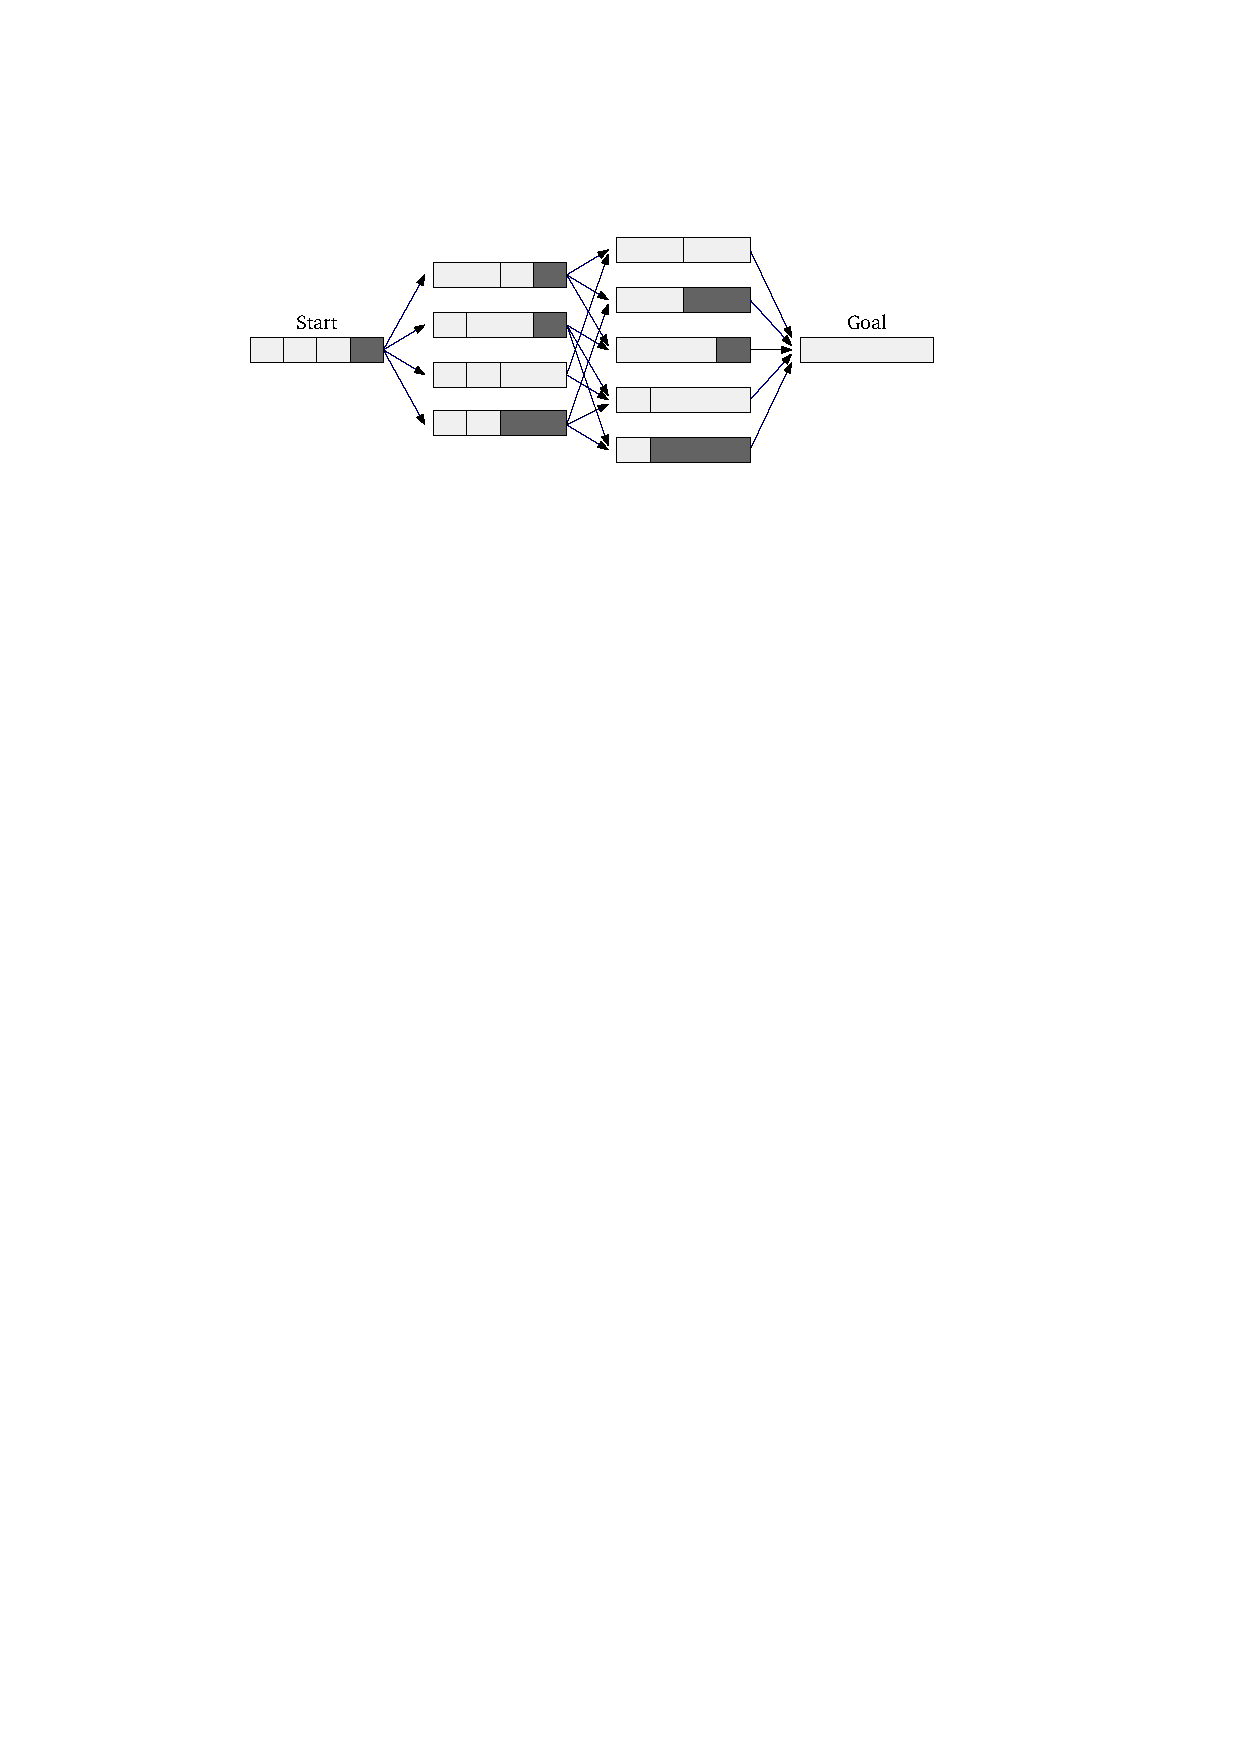
\includegraphics[page=1]{Intro}
\caption{There are many ways of aggregating 
a set of land-cover areas to a single one.}
\label{fig:Intro_SubdivisionName}
\end{figure}

Optimization has been widely used in map generalization.
For example, \textcite{Harrie1999} displaced objects 
based on least-squares adjustments (LSA)
to solve spatial conflicts.
In his problem, the soft constraints 
for shapes and locations may contradict each other.
Therefore, it is necessary 
to mediate between these constraints, 
which can be done by LSA.
\textcite{Sester2005Optimization} used LSA not only for 
displacing objects but also for simplifying buildings. 
She required that 
the output boundaries should be 
as close to the original buildings as possible.
\textcite{Tong2015AreaLSA} generalized land-cover areas,
where LSA was used to preserve the sizes of 
the land-cover areas.
\textcite{Regnauld2001} grouped buildings based on 
minimum spanning trees in order to typify
the buildings in a group.
\textcite{Burghardt2005Snakes} smoothed lines based on 
energy minimization. 
According to his setting, a line contains less energy
if it is smooth and close to the original line.
He repeatedly displaced the line 
until finding a stable state 
in terms of minimizing his energy function.
\textcite{HaunertWolff2010AreaAgg} aggregated land-cover areas
based on mixed-integer linear programming.
This method is based on global optimization and minimizes 
type changes as well as a cost for non-compact shapes 
while satisfying constraints on the sizes of the output regions.
\textcite{Haunertwolff2010Building} simplified building
footprints by solving an integer linear program (ILP).
They aimed at minimizing the number of edges in the output 
under the restriction that 
the simplified buildings must be topologically safe,
that is, the selected and extended edges must not intersect with 
each other.
\textcite{Oehrlein2017Aggregation} aggregated the departments 
of France according to unemployment rates based on integer 
linear programming; they used a cutting-plane method to 
speed up solving their ILP.
\textcite{Funke2017Simplification} simplified 
administrative boundaries based on an ILP.
Their aim was to minimize the number of edges
while keeping the result boundaries close to the original ones
and avoiding any intersection. 
At the same time, they required that every city, 
represented by a point, 
stays in the same face as before the generalization.



\mypar{Optimization in \emph{continuous} map generalization}
Optimization becomes more delicate
when we deal with CMG.
In this field, we have requirements 
not only for a specific map
but also for relations between maps at difference scales. 
%
Some optimization techniques have been applied to CMG.
In the aforementioned article,
\textcite{Noellenburg2008} used dynamic programming
to match points of two polylines to support morphing
according to some matching cost.
\textcite{sahw-oarps-ICAGW13} used 
mixed-integer linear programming 
to select points of interest.
They required that a point, once disappeared, 
should not show up again during zooming out. 
They also required that any two points should be 
sufficiently far away from each other.
Based on these requirements, 
they wanted to show as many points as possible 
for a given scale interval.
\textcite{Chimani2014Eat} computed a deletion sequence
for a road network by integer linear programming
and efficient approximation algorithms.
They wanted to delete a stroke, 
which is a sequence of edges, at each step
while keeping the remaining network connected.
They assigned each edge a weight, 
and their objective was to maximize the total weight 
over all the road networks of all the steps.
%\textcite{Peng2013LSA} defined trajectories 
%based on LSA for morphing between polylines, 
%where LSA is used to mediate between the requirements 
%for angles and edge lengths of the intermediate polylines.

\section{Tools for Optimization}
\label{sec:Intro_Tools}

In this thesis, we use some well-known optimization methods,
namely, the \Astar algorithm \parencite{Hart1968}, 
integer linear programming
\parencite[chapter~13]{Papadimitriou1982combinatorial},
dynamic programing \parencite[chapter~15]{Cormen2009}, and
least-squares adjustment (LSA) \parencite[chapter~3]{Koch1988}.
We also use the minimum spanning tree;
see \textcite[chapter~23]{Cormen2009}.
%
We use \Astar and integer linear programming 
to find optimal sequences for 
area aggregation (see \chap\ref{chap:AreaAgg}).
Similar to \textcite{Noellenburg2008},
we use dynamic programming to 
compute corresponding points between polylines
(see \chaps\ref{chap:Admin} and \ref{chap:Morph}).
We use the minimum spanning tree to group buildings,
which is similar to \textcite{Regnauld2001}; 
see \chap\ref{chap:Bldg}.
We define trajectories based on LSA 
for morphing between polylines (see \chap\ref{chap:Morph}).
% There is no optimization used in \chap\ref{chap:DataStr}.
In the following, we briefly recall these methods.


Given a graph with nodes and weighted edges,
a typical task is to find a shortest path 
from a start node to a goal node.
A breadth-first search \parencite[chapter~22]{Cormen2009}
solves the shortest-path problem 
in unweighted graphs.
Dijkstra's algorithm \parencite{Dijkstra1959}
always chooses from the explored nodes the neighbor 
with minimum distance from the start node. 
The \Astar algorithm is 
a generalized version of Dijkstra's algorithm.
When \Astar chooses a node to explore the neighbors,
the algorithm does not only take into account 
the distance from the start node
but also estimates the distance to the goal node.
By always choosing a node which is likely 
to be closer to the goal node, 
\Astar often explores fewer nodes than Dijkstra's algorithm
in finding a shortest path.
If the estimated distances are always smaller than the exact 
distances to the goal node, 
then \Astar will find a shortest path.

Linear programming models an optimization problem as objective 
functions subject to constraints,
where the objective functions and constraints are represented by 
linear functions of some variables.
These constraints form a convex polyhedron.
An optimal solution lies on the boundary of the polyhedron and 
can be found efficiently.
\emph{Integer} linear programming requires that
the variables must use integers.
Integer linear programming is NP-hard
since many NP-hard problems such as vertex cover can be 
formulated as integer linear programs.
Intuitively, this is due to the fact that the optimal solution 
may lie in the interior of the polyhedron, where geometry does 
not help to find it.
If only some of the variables are required to be integers
(other variables are allowed to be non-integers), 
then the problem is called mixed integer linear programming,
which is also known as NP-hard; see for more details
\textcite[chapter~16]{Schrijver1986}.



Dynamic programming decomposes 
a big instance of a complex problem 
into a collection of smaller subinstances.
The method solves each subinstance just once 
and saves the solution. 
The next time when the same subinstance occurs, 
the method will use the previously computed solution 
instead of resolving this subinstance. 
In this way, the method saves computation time.
Other than in the divide-and-conquer approach used, 
e.g., in Mergesort, 
in dynamic programming subinstances of equal size 
are usually \emph{not} disjoint but overlap.

Least-squares adjustment is a model for solving 
over-constrained problems.  
It handles computes a set of unknowns 
based on a set of observations.
Because of errors, the observations may contradict each other.
We have to adjust the observations 
so that we can obtain a set of unknowns that agree 
all the adjusted observations.
There can be infinitely many sets of adjustments feasible, 
but we choose the one with the least sum of squared adjustments.
Based on this set of adjustments,
we can finally compute the unknowns.


Given a graph with nodes and weighted edges, 
a minimum spanning tree (MST) of the graph 
is a minimum-weight subset
of the edges that together connect all nodes.
Surprisingly, the MST can be computed 
by simple greedy algorithms
such as Kruskal's algorithm \parencite{Kruskal1956}
or the algorithm of Jarn\'ik--Prim 
\parencite{Jarnik1930,Prim1957}.
Strictly speaking, the MST by itself is not 
an optimization \emph{method}, 
but it is a helpful structure of low weight 
that helps to solve many optimization problems 
in graph theory at least approximately, 
for example, the metric version of the famous Traveling
Salesperson Problem (TSP).


\section{Overview of the Thesis}
\label{sec:Intro_Overview}

This thesis contains five chapters 
that deal with methods for continuous map generalization. 
First, we find optimal sequences 
for aggregating land-cover areas.
%
Second, we continuously generalize county boundaries to
provincial boundaries.
%
Third, we continuously generalize buildings to built-up areas 
by aggregating and growing.
%
Fourth, we define moving trajectories
based on least-squares adjustment
for morphing between polylines.
%
Fifth, we discuss the performance 
of data structures for spatial problems.
%
In the remainder of this section, 
we present our results in more detail.


\subsubsection{%
Finding Optimal Sequences for Area Aggregation---\\
\Astar vs. Integer Linear Programming}

To provide users with maps of different scales and 
to allow them to zoom in and out without losing context,
automatic methods for map generalization are needed.
We approach this problem for land-cover maps.
%Given two maps of the same region at two different scales,
%a relevant problem is to compute maps for any intermediate scale.
Given two land-cover maps at two different scales, 
we want to find a sequence of small incremental
% To help map users not to lose context during zooming,
% we try to provide maps that change as continuous as possible.
% Since maps at some different scales often exist, 
% a relevant problem is to find maps at any intermediate scales.
% Given two land-cover maps of different scales, 
% we wish to find a sequence of small incremental
changes that gradually transforms one map into the other.
We assume that the two input maps consist of polygons 
each of which belongs to a given land-cover class. 
Every polygon on the smaller-scale map
is the union of a set of adjacent polygons 
on the larger-scale map. 

In each step of the sequence that we compute, 
the smallest area is merged with one of its neighbors. 
We do not select that neighbor according to a prescribed rule 
but compute the whole sequence of pairwise merges at once, 
based on global optimization.
We formalize this optimization problem as that of 
finding a shortest path in a (very large) graph.
%We compared the \Astar algorithm and 
%integer linear programming in solving this problem.
For solving such a problem, standard approaches
are the \Astar algorithm or integer linear programming.
%We compare how the two methods solve our problem.
To avoid long computing times, we allow the two methods to 
return non-optimal results.
In addition, we present a greedy algorithm 
as a benchmark.
We tested the three methods with a
dataset of the official German topographic database ATKIS.
Our main result is that
\Astar finds optimal aggregation sequences for more instances 
than the other two methods
within a given time frame.
\fig\ref{fig:Intro_AreaAgg_Case612} shows some intermediate 
results obtained by \Astar for one of the regions.
This is joint work with Alexander Wolff and Jan-Hendrik Haunert,
part of which has been published~\parencite[see][]{Peng2017AStar}.


\begin{figure}[tb]
\centering
\includegraphics[page=2]{Intro}
\caption{Some intermediate aggregation results of 
	a region (Buchholz in der Nordheide, Germany). 
	There are $9$ polygons on 
	the larger-scale map (top left). 
	These areas are aggregated into one 
	on the smaller-scale map (bottom left). 
	The digits are the numbers of the areas.
}
\label{fig:Intro_AreaAgg_Case612}
\end{figure}

\subsubsection{%
Continuously Generalizing Administrative Boundaries\\
Based on Compatible Triangulations}

Topological consistency is a key issue 
in cartographic generalization.
Our aim in this chapter is to ensure topological consistency  
during continuous map generalization 
of administrative boundaries.
To this end, we present a five-step method.
Our inputs are two maps of administrative boundaries 
at different scales, 
where the larger-scale map has not only more details 
but also an additional level of administrative regions.

Our main contribution is the proposal of a workflow for
generalizing hierarchical administrative boundaries in a
continuous and topologically consistent way.  First, we
identify corresponding boundaries between the two maps.
We call the remaining boundary pieces (on the larger-scale map)
\emph{unmatched} boundaries.  
Second, for the unmatched boundaries,
we generate their corresponding boundaries 
on the smaller-scale map
based on compatible triangulations. 
Third, we simplify the generated boundaries
by Douglas--Peukcer algorithm.  
Fourth, we compute corresponding points for each pair
of corresponding boundaries using a variant of an existing 
dynamic programming algorithm.  
Fifth, we interpolate between the corresponding points
to generate the boundaries at intermediate scales.

We do a thorough case study 
on the provincial and the county boundaries of Mainland China.
Although topologically consistent algorithms 
for the third step and the fifth step exist, 
we have implemented simpler algorithms for our case study. 
\fig\ref{fig:Intro_AdminBound_Tianjin} shows our results of 
continuously generalizing county boundaries 
to provincial boundaries of Tianjin, China.
This is joint work with Alexander Wolff 
and Jan-Hendrik Haunert~\parencite[see][]{Peng2016Admin}.

\begin{figure}[tb]
\centering
\includegraphics[page=3]{Intro}
\caption{Continuously generalizing county boundaries to 
provincial boundaries of Tianjin province, China.}
\label{fig:Intro_AdminBound_Tianjin}
\end{figure}

\subsubsection{%
Continuously Generalizing Buildings to Built-up Areas\\
by Aggregating and Growing}

To enable smooth zooming, 
we propose a method to continuously generalize buildings 
from a given start map to a smaller-scale goal map, 
where there are only built-up area polygons 
instead of individual building polygons
(see Figure~\ref{fig:Intro_BldgGrow}).
We name the buildings on the start map 
\emph{original buildings}.
%
For an intermediate scale, 
we aggregate the original buildings that will become too close 
by adding bridges.
We grow the (bridged) original buildings based on buffering 
and simplify the grown buildings.
We take into account the shapes of the buildings 
on both the preceding map and the goal map to make sure that 
the buildings are always growing.
The running time of our method is in~$O(n^3)$,
where~$n$ is the total number of edges
overall the original buildings.
%

The advantages of our method are as follows. 
First, we grow the buildings continuously 
and, at the same time, simplify the grown buildings.
Second, right angles of buildings are preserved during growing: 
the merged buildings still look like buildings. 
Third, the distances between buildings are 
always larger than a specified threshold.
We do a case study to show the performances of our method.
This is joint work with 
Guillaume Touya~\parencite[see][]{Peng2017Building}.

\begin{figure}[tb]
\centering
\includegraphics[page=4]{Intro}
%\includegraphics[page=4]{Bldg_CaseStudy_DataAndResults}
\caption{Continuously generalizing buildings to built-up 
	areas by aggregating and growing.}
\label{fig:Intro_BldgGrow}
\end{figure}


\subsubsection{Morphing Polylines 
	Based on Least-Squares Adjustment}

One way of continuously generalizing polylines 
is to use morphing techniques. 
Most often for morphing, 
the vertices of the polylines move on 
defined straight-line trajectories at constant speeds.
In this chapter we address morphing of polylines, 
but we relax the requirement that 
the vertices of the polylines move on straight lines. 
Our concern with straight-line trajectories is that 
characteristic properties (e.g., bends) of the polylines 
change drastically during the morphing process. 
In particular, we suggest that 
the angles and the edge lengths of the polylines 
should change linearly during the morphing process. 
This expectation is clearly not accomplished 
with straight-line trajectories. 
In contrast, we present a new method 
based on least-squares adjustment 
that yields close-to-linear changes of 
the angles and the edge lengths. 
Figure~\ref{fig:Intro_LSA_Compare} 
shows a comparison of morphing based on 
straight-line trajectories and our new morphing method.
This is joint work 
with Jan-Henrik Haunert, Alexander Wolff, 
and Christophe Hurter~\parencite[see][]{Peng2013LSA}.

\begin{figure}[htb]
\centering
\includegraphics[page=2]{Morph_CaseStudy_Artificial}
\caption{A comparison of morphing 
    based on the two different trajectories.}
\label{fig:Intro_LSA_Compare}
\end{figure}

\subsubsection{Choosing the Right Data Structures 
	for Solving Spatial Problems}

When we plan to implement a program, 
there are always many data structures that
we can use to achieve a certain goal.
However, if we do not carefully choose and use 
the data structures,
the implemented program may be inefficient.
As an example, we consider the problem of 
finding pairs of close points from a dataset. 
We consider two points to be close 
if they lie within a square of pre-specified 
side length~$\varepsilon$. 
We compare three obvious algorithms to solve the problem: 
a sweep-line (SL) algorithm, 
an algorithm based on the Delaunay triangulation (DT) 
of the input points, 
and a hashing-like algorithm 
which overlays the input points with a rectangular grid. 
We implemented the algorithms in C\# and tested them on 
randomly generated data and real-world data. 
We used the DT available in ArcGIS Objects. 
We used three different data structures
of \emph{balanced binary search} tree, 
i.e., SortedDictionary (SD), SortedSet (SS), and TreeSet (TS), 
to implement the sweep-line algorithm. 
The simple grid-based algorithm turned out to run faster than 
any of the other algorithms by a factor of at least~$2$ 
(see Figure~\ref{fig:Intro_DataStructure}).
This is joint work with 
Alexander Wolff~\parencite[see][]{Peng2014DataStr}.

%\bigskip
%The thesis is closed with a summary and a list of open problems.

\begin{figure}[tb]
\centering

\includegraphics[page=2]{DataStr_Plot_Bavaria}
\caption{Time consumption of the algorithms
	for computing close point pairs. 
	Two points are defined as close if the differences 
	of their $x$- and $y$- coordinates are both smaller than
	$\varepsilon=0.001267 \degree$,
	where the coordinates are with unit degree. 
	The DT-based algorithm took $262\,$s 
	with radius $r_1=\varepsilon \cdot (1+\sqrt{2})/2$ 
	("DT $r_1$") and $784\,$s 
	with radius $r_2=\varepsilon \cdot (1+\sqrt{7})/2$ 
	("DT $r_2$") for $n=553{,}984$ points.
	The curve labeled "DT constr." represents 
	the time for constructing 
	Delaunay triangulations for the input points.
}
\label{fig:Intro_DataStructure}
\end{figure}


\section{Acknowledgments}

Obtaining a Ph.D.\ in Germany was 
one of the best things I~could dream of.
When I~finally got the chance to study in Germany,
I~was thrilled and I~wanted to do my best.
Now I~feel so proud of myself because I~have come this far.
Of course, this thesis would not have been possible
if it were not for the help of many people.

First of all, I~would like to thank my supervisor, 
Prof.\ Dr.\ Alexander ``Sascha'' Wolff.
I~am grateful to him for giving me 
the opportunity to pursue my Ph.D.\ in his group.
The research work was challenging,
but I~enjoyed working with him.
Sascha has been very patient with me.
When I~first came to Germany, I~could barely speak English.
He had to put a lot of effort into understanding me
when we were doing research.
Sascha advised me to take lectures and sent me to conferences
so that I~could learn as much as possible.
Sascha always encouraged me to ask questions
because I~can benefit from the answers.
He told me not to be shy even when 
I~fear that the questions are stupid;
other people in the audience may appreciate my asking
because they may have the same questions,
but don't dare to ask.
%% Here, the point is not so clear (and not so exciting); I'd drop it.
% Sascha always responded my requests promptly.
% Once, I~noticed that I~was missing a letter from him 
% for some business on the next day
% while he was attending a conference in Italy.
% Nevertheless, after I~had written him an email,
% he sent me the letter before 20:00.
At some point,
Sascha even negotiated with my landlords 
when I~moved from an apartment into another.
Moreover, Sascha has a good sense of humor, 
and we often cracked jokes together.
I~was lucky to have him as my supervisor.

I~also thank my second supervisor, 
Prof.\ Dr.\ Jan-Henrik Haunert.  
In his lecture \emph{Algorithms for GIS}, 
he taught me many fundamentals of GIScience.  
Later, he moved to other universities 
and invited me to visit him there.
During the visits, we sketched many ideas together.
In particular, he proposed % the research of 
using the \Astar algorithm 
for finding optimal sequences for area aggregation,
which led to the most important chapter of my thesis.
Furthermore, he recommended many suitable conferences to me
when I~wanted to publish my papers.
% He taught me the ``optimization mantra'' (explain?).
% DP: I~do not understand ``optimization mantra''
% AW: A "mantra" is a sequence of words that are repeated over and
% over because they are so important:
% https://en.wikipedia.org/wiki/Mantra
% Mantras [....] helps to induce an altered state of consciousness.
% :-)

I~am grateful to all the colleagues in our group:
Moritz Beck, Johannes Blum, Benedikt Budig, 
Steven Chaplick, Thomas van Dijk, 
Martin Fink, Oksana Firman, Krzysztof Fleszar, 
Philipp Kindermann, Myroslav Kryven, 
Fabian Lipp, Andre L\"offler, 
Nadine Schwartges, Joachim Spoerhase, Sabine Storandt, 
and Johannes Zink.
%
We often had coffees together,
and it was a lot of fun to play squash and to go out for our excursions.
It was nice that our group always had lunch together
so that we had plenty of chances to learn from each other.
Indeed, I~sometimes took advantage of these lunches
to get suggestions regarding my research work.
%
I~am also grateful to Sigrid Keller.
She found an apartment for me 
before I~arrived Germany.
Then, she picked me up at the train station of W\"urzburg
and brought me to that apartment.
She was very kind to me 
and helped me to fill many forms related to my Ph.D.\ study.


I~am indebted to Dr.\ Krzysztof Fleszar for 
helping me a lot during my Ph.D.\ study.
He is very warm-hearted.
Whenever he found that I~had problems to understand a paper,
he read that paper and then explained it to me.
He always helped when I~needed a German--English translator.
He helped me move twice using the van of his family.
On the day before my defense, he worked as hard as me
in order to give me feedback about my slides.
He has always invited me to join his parties, 
and I~am grateful for his invitations.

I~thank Dr.\ Guillaume Touya for inviting me to visit
the French National Mapping Agency (IGN).
The visit was a great chance and gave me insight into
practical requirements regarding maps.
Our collaboration resulted in a paper on continuously
generalizing buildings into built-up areas.
%
I~also thank Dr.\ Thomas van Dijk.
He helped me speed up my 
least-squares adjustment using \emph{Eigen}, a C++ library.
He has proofread some of my papers
and has given me helpful suggestions 
concerning many aspects of my research.

I~am grateful to Prof.\ Dr.\ Min Deng,
the supervisor of my master's study.
He introduced me into the research area of 
continuous map generalization 
and helped me to get the chance of
pursuing my Ph.D.\ at the University of W\"urzburg.
Under his supervision,
we coauthored some nice papers.


I~thank Prof.\ Dr.\ Dirk Burghardt 
for reviewing my thesis within a short time frame
when my working contract in W\"urzburg was about to end.
I~also thank him for introducing my research work to
Prof.\ Dr.\ Peter van Oosterom, 
which certainly helped me to get a postdoc position
in Peter's group.
Before submitting the final version of my Ph.D.\ thesis,
I~have already been working in Peter's group.
I~would like to thank Peter and Dr.\ Martijn Meijers 
for allowing me to finish my paper about area aggregation,
which is part of this thesis. 
I~thank Prof.\ Dr.\ Andreas N\"uchter for chairing my defense.

I~would like to thank my parents
for all their love and encouragement.
I~thank them for their suggestions 
when I~was making decisions.
My special thanks go to Fang Wu.
She has been very supportive of me.
We enjoyed many activities together, 
including hiking, skating, skiing, shopping, and so on.
She made my life much more colorful.

I~thank all my friends in W\"urzburg
for their company.
Because of them, I~could better explore the city 
and even the whole country.

Last but not least, 
I~am very grateful to the University of W\"urzburg 
because I~had the opportunity to take many courses.
In order to gain sufficient credits for 
obtaining a Ph.D.\ degree in Computer Science,
I~took some courses
(e.g., \emph{Theoretical Computer Science}
and \emph{Algorithms and Data Structures})
in my own faculty, 
the Faculty of Mathematics and Computer Science.
%
In order to improve my language skills,
I~took many courses
offered by the Language Center
(e.g., \emph{English for the Natural Sciences} 
and \emph{General Language Exercise of German})
and by the Faculty of Arts 
(e.g., \emph{Introduction to English Linguistics}).

%}
%\chapter[<ToC-title>]{<Title>} 
\chapter[\AreaAggToCTitle]{\AreaAggTitle} 
\label{chap:AreaAgg}
%appear at the top of the pages
\chaptermark{\AreaAggChapterMark}

The land-cover area is of significant importance on maps.
When users zoom out, some land-cover areas become
too tiny to be seen, which result in visual clutter.
In order to provide users 
with good visual experience during zooming operations,
we propose to remove these tiny areas.
We plan to achieve this goal by 
aggregating them into neighboring land-cover areas.
A \emph{land-cover map} is a planar subdivision in which 
each area belongs to a land-cover class or \emph{type}.
Suppose that there are two land-cover maps of different scales 
that cover the same spatial region.
We consider the problem of finding a sequence 
of small incremental changes that gradually transforms 
the larger-scale map (the \emph{start map}) to 
the smaller-scale map (the \emph{goal map}).
We use this sequence to generate and show land-cover maps at 
intermediate scales (see \fig\ref{fig:AreaAgg_example}).
In this way, we try to avoid large and discrete changes
during zooming.

With the same motivation, 
a strategy of hierarchical schemes has been proposed.
This strategy generalizes a more-detailed representation 
to obtain a less-detailed representation 
based on small incremental changes, 
e.g., the Generalized Area Partitioning tree (GAP-tree).
This tree can be constructed if only the larger-scale map is given
\citep{vanOosterom2005} 
or if both the larger-scale map and the smaller-scale map 
are given \citep{HaunertDilo2009}.
Typically, the next change in such a sequence 
is determined locally, in a greedy fashion.  
If we insist on finding a sequence that is optimal 
according to some global measure,
the problem becomes complicated.

\begin{figure}[tb]
\centering
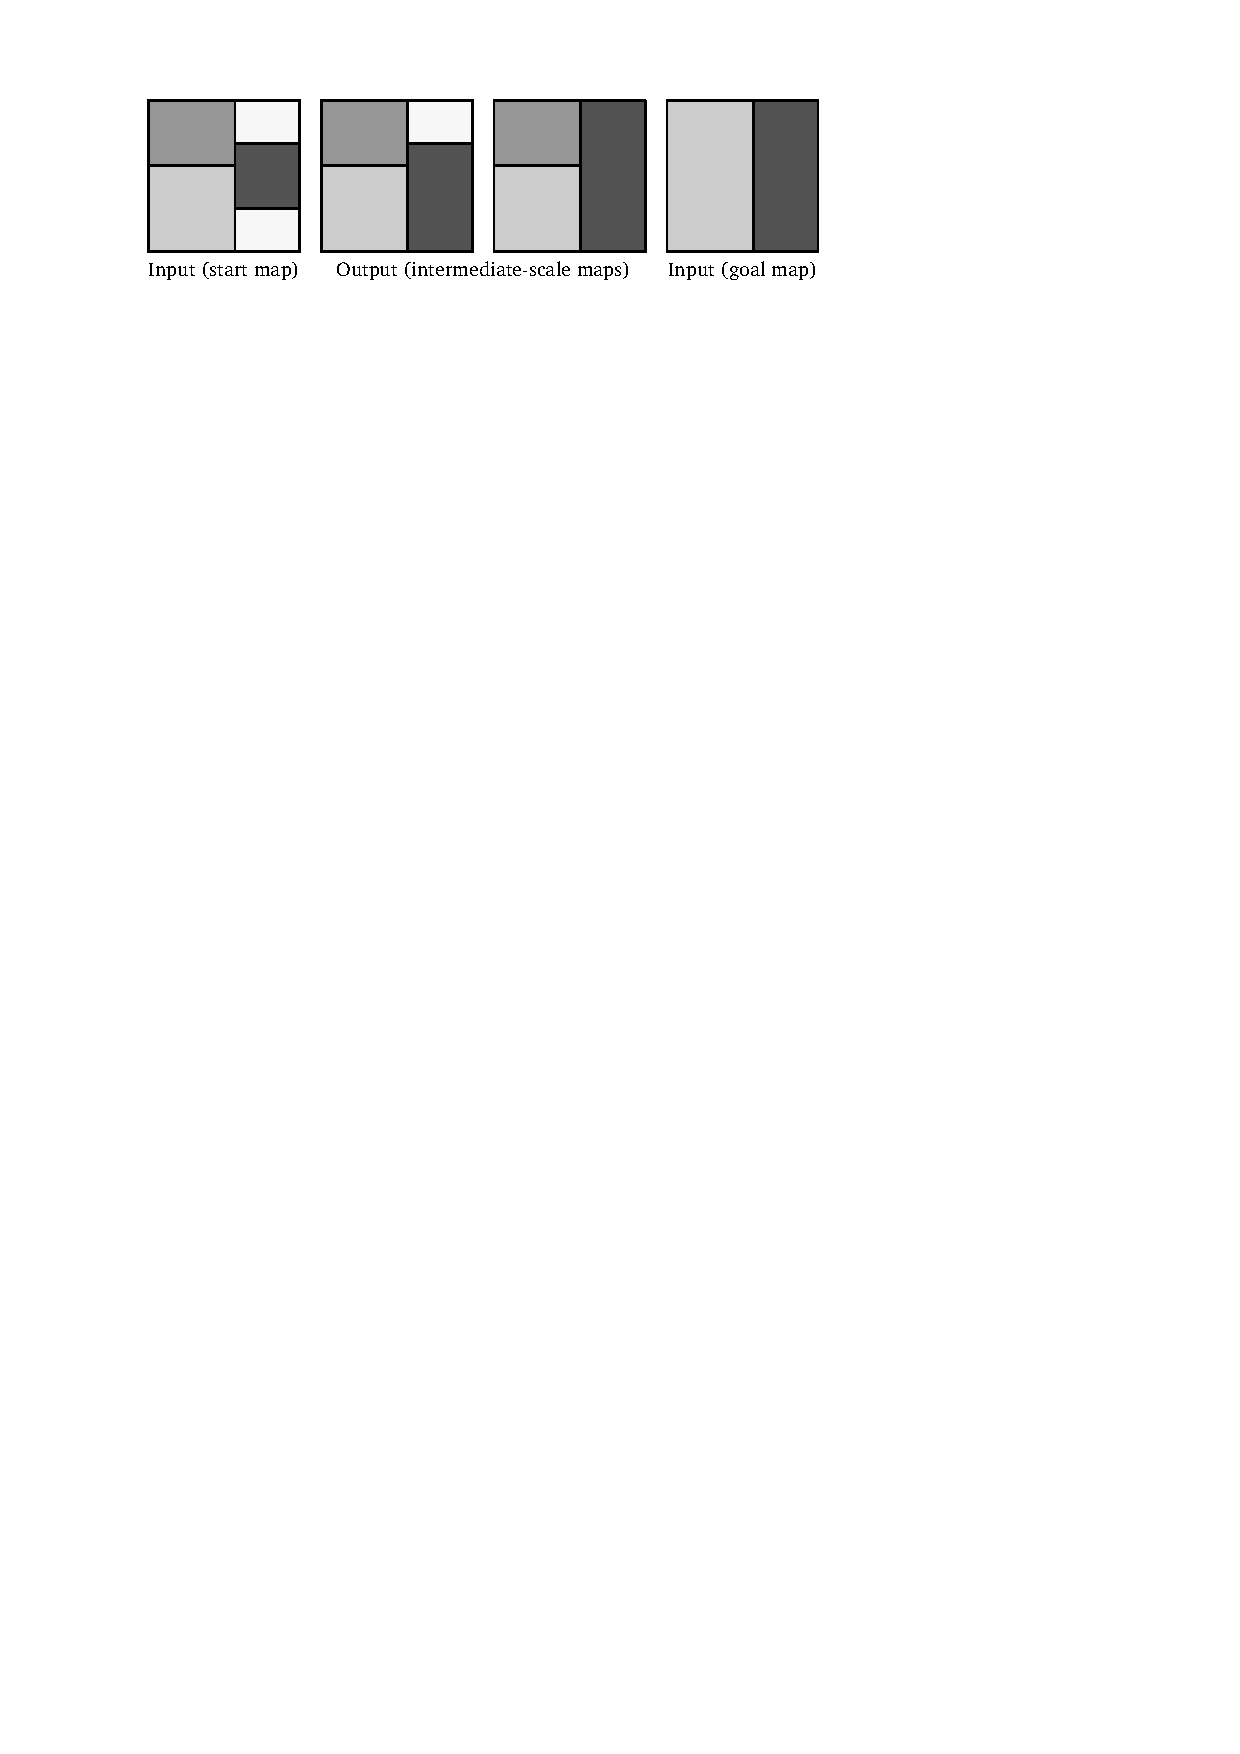
\includegraphics[page=1]{AreaAgg_Preliminaries}
\caption{The input and a possible output for an instance of 
our problem.}
\label{fig:AreaAgg_example}
\end{figure}

We assume that there exist many-to-one relationships 
between the areas of the start map and the areas of the goal map.
This assumption is based on the fact that many algorithms 
\parencite[e.g.,][]{HaunertWolff2010AreaAgg,
vanSmaalen2003,Oehrlein2017Aggregation}
result in many-to-one relationships
when aggregating land-cover areas.
Their inputs and generalized results together
can be used as our inputs.
However, we should not use those algorithms
to generate a sequence of maps at different scales
because those algorithms do not take into account 
the consistence between the generated maps.
We use both a start map and a goal map instead of using only the start map
because our generated maps at intermediate scales should be able to
benefit from a goal map with high quality.
We term the areas of the goal map \emph{regions}.
That is, every region is the union of a set of areas 
on the start map.
The type of a region may differ from the types of its 
components. 
For example, a small water area together with 
multiple adjacent forest areas may constitute 
a large forest region on the smaller-scale map.
However, we assume that every region, on the goal map, 
contains at least one area of the same type on the start map.
Our assumptions hold if the goal map has been produced 
with an automatic method for area aggregation, 
for example, by the method of \citet{HaunertWolff2010AreaAgg}.
That method produces a land-cover map at a single smaller scale, 
given a land-cover map at a larger scale.
Although \textcite{HaunertWolff2010AreaAgg}
attain results of high quality, 
they do not produce a sequence of land-cover maps.

Our method can also be extended to find an aggregation sequence 
for two maps (a start map and a goal map) that are from different sources.
In that case, one could compute a map overlay of the two maps
and use the result 
(with combined boundaries from both input maps and land cover classes 
from the given large-scale map) 
as the start map.

In this chapter, we try to find an optimal sequence
to aggregate the land-cover areas on the start map
one by one until we arrive at the goal map.
We first independently deal with each region of the goal map 
(with its components on the start map).
Once we have found an aggregation sequence for each region, 
we integrate all the sequences into an overall sequence,
which transforms the start map into the goal map
(see \fig\ref{fig:AreaAgg_IntegrateSequence}). 
Our aggregation sequence may be cooperated with
the GAP-face tree \citep{vanOosterom2005},
the map cube model \citep{Timpf1998},
or ScaleMaster \citep{Brewer2007Guidelines,Touya2013ScaleMaster}, 
to support on-the-fly visualization.
Smoothly (dis-)appearing areas can be realized
by integrating our results into the \emph{space-scale cube}
\parencite{vanOosterom2014tGAP,vanOosterom2014tGAPSSC}.

\begin{figure*}[h]
\centering
\includegraphics[page=2]{AreaAgg_Preliminaries}
\caption{Integrating two aggregation sequences 
	of different regions: 
	the resulting sequence contains the given sequences 
	as subsequences and 
	always takes the subdivision with smallest patch next.
	The gray arrows show the integration of the two regions.
}
\label{fig:AreaAgg_IntegrateSequence}
\end{figure*}

\mypar{Contribution}
We formally model our problem, 
analyze the size of our model in a worst-case scenario,
introduce our methods,
and present the basic concepts of our method
(\sect\ref{sec:AreaAgg_Preliminaries}).
We define our cost functions 
(\sect\ref{sec:AreaAgg_CostFunctions}).
We prove that our problem is NP-hard
(\sect\ref{sec:AreaAgg_NP-hardness}).
Then, we develop and compare three methods 
for finding aggregation sequences.
First, we present 
a greedy algorithm (\sect\ref{sec:AreaAgg_Greedy}).
Second, we develop a new global optimization approach
based on the \Astar algorithm 
(\sect\ref{sec:AreaAgg_AStar}).
Third, we model our pathfinding problem as
an \emph{integer linear program} (ILP), 
and we solve this ILP with minimizing our cost function
(\sect\ref{sec:AreaAgg_ILP}).
Our ILP uses binary (0--1) variables. 
These variables help us to model our problem, 
but in general, it is NP-hard 
to solve an ILP optimally.
By comparing with the greedy algorithm, 
which is used as a benchmark,
we are able to see whether \Astar or the ILP-based algorithm, 
which are more complex and slower, indeed perform better.  
Our case study 
uses a dataset of the German topographic database ATKIS 
(\sect\ref{sec:AreaAgg_CaseStudy}).
In the concluding remarks, we show possible ways to improve our 
methods (\sect\ref{sec:AreaAgg_Conclusions}). 




We do not deal with simplifying polylines in this chapter.
The simplification can be handled separately from the
aggregation of areas by using one of the existing methods
\parencite[e.g.,][]{Douglas1973,Saalfeld1999,Wu2004DP}.
Those methods can be used to set up 
the binary line generalisation tree (BLG-tree) of
\textcite{vanOosterom1995Development},
which is a hierarchical data structure that 
defines a gradual line simplification process.
%
Although splitting polygons is a good step
of generalizing land-cover areas,
we do not integrate it into our method at this moment.
Some examples of splitting are as follows.
\textcite{Smith2007MasterMap,Thiemann2018LandCover} 
proposed to split tiny polygons 
and then to merge the split parts into the neighboring polygons.
\textcite{Meijers2016Split} developed an algorithm 
to split a polygon (the splittee) 
based on a constrained Delaunay triangulation.
During splitting, their algorithm is capable of
taking into account
the attractivenesses between the splittee and its neighbors.
When merging, a more attractive neighbor 
will get a larger portion from the splittee.


\section{Preliminaries}
\label{sec:AreaAgg_Preliminaries}

We show how to compute an aggregation sequence 
for a single region, $R$. 
For a goal map with many regions,
we ``interleave'' the sequences for each of them
with respect to the order of the smallest patches 
(see for example \fig\ref{fig:AreaAgg_IntegrateSequence}).
This integration is similar to the merge step in the 
Mergesort algorithm; 
see \textcite[\sect2.3]{Cormen2009}.
To allow us to describe our method more easily,
below we assume that the goal map has only one region.
This region consists of~$n$ land-cover 
areas (components) on the start map. 
In other words, the union of the~$n$ land-cover areas 
is the only region on the goal map.



To find a sequence of small changes 
that transforms the start map into the goal map,
we require that 
every change involves only two areas of the current map.
More precisely, in each step the smallest area~$u$ is merged 
with one of its neighbors~$v$ 
($v$ does not have to be the smallest neighbor)
such that~$u$ and~$v$ are replaced by their union.
The type of the union is restricted to be 
the type of either~$u$ or~$v$.
If the union uses the type of~$u$, 
we say that area~$v$ is \emph{aggregated into} area~$u$, 
and vice versa. 
How to aggregate exactly is decided by 
optimizing a global cost function
(see \sect\ref{sec:AreaAgg_CostFunctions}).
This requirement ensures that the 
size of the smallest area on the map increases in each step.
Hence, the sequence reflects a gradual reduction of the 
map's scale.
From another perspective, 
we consider the smallest area as the least important, 
rather than involving more rules for (non-)importance. 
Even though the requirement reduces 
the number of possible solutions,
there is still enough room for optimization 
since we leave open with
which of its neighbors the smallest area is aggregated.
We term a sequence of changes 
that adheres to our smallest-first requirement simply 
an \emph{aggregation sequence}.


\subsection{Model}
\label{sec:AreaAgg_Model}
We consider a directed graph $G_\mathrm{S}$, 
which we call the \emph{subdivision graph} 
(see \fig\ref{fig:AreaAgg_SubdivisionName}). 
The node set $V_\mathrm{S}$ of~$G_\mathrm{S}$ 
contains nodes for all the
possible maps (or \emph{subdivisions}), including the start map, 
all possible intermediate-scale maps, and the goal map.
The arc set~$E_\mathrm{S}$ of~$G_\mathrm{S}$ 
contains an arc $(\Pnode, P_{t+1,j})$ 
between any two maps~$\Pnode$ and~$P_{t+1,j}$ in~$V_\mathrm{S}$ 
if~$P_{t+1,j}$ can be reached from~$\Pnode$ 
with a single aggregation operation,
involving a smallest area.
On this basis, any directed path in~$G_\mathrm{S}$ 
from the start map to the goal map
defines a possible aggregation sequence.

\begin{figure}[h]
\centering
\includegraphics[page=3]{AreaAgg_Preliminaries}
\caption{The subdivision graph, $G_\mathrm{S}$. 
	The nodes of the graph are the subdivisions. 
	There is an arc	from subdivision~\Pnode 
	to subdivision~${P}_{t+1,j}$ 
	if~${P}_{t+1,j}$ is the result of 
	an aggregation step from~\Pnode.}
\label{fig:AreaAgg_SubdivisionName}
\end{figure}


\subsection{Notation}
\label{sec:AreaAgg_Notation}

We represent each land-cover area by a polygon with a type.
We denote by~$P$ the set of polygons on the start map.
We use~$p$, $q$, $r$, or~$o$ to denote polygons.
A \emph{patch} is a set of polygons whose union is connected. 
Each patch also has a unique land-cover type.
We use~$u$ or~$v$ to denote the patches.

Recall that we are dealing with a single region and 
there are~$n$ land-cover areas on the start map in this region. 
Hence, the desired aggregation sequence consists of~$n-1$ steps. 
There are~$n$ subdivisions on a path 
from the start map to the goal map. 
We use~$t \in T =\{1,2,\dots,n\}$ to denote \emph{time}. 
When~$t=1$, the subdivision consists of~$n$ patches, 
and there is only one patch remaining when~$t=n$.
The subdivision graph consists of layers~${L}_1,\dots,{L}_n$, 
where layer~${L}_t=\{{P}_{t,1},\dots,{P}_{t,n_t}\}$
contains every possible subdivision~\Pnode\ with~$n-t+1$ patches 
(see \fig\ref{fig:AreaAgg_ExponentialSize}).


\begin{figure}[tb]
\centering
\includegraphics[page=4]{AreaAgg_Preliminaries}
\caption{An example to show that 
    the size of subdivision graph~$G_\mathrm{S}$
	has exponential lower bound.}
\label{fig:AreaAgg_ExponentialSize}
\end{figure}

Sometimes, we need a graph to represent the adjacencies of
the land-cover areas in a subdivision,
we call such a graph~$G_\mathrm{A}$
(see \fig\ref{fig:AreaAgg_Variables_Graph}). 


\begin{figure}[tb]
\centering
\includegraphics[page=3]{AreaAgg_ILP}
\caption{The adjacency graph of a subdivision,~$G_\mathrm{A}$.
	Each polygon of the subdivision is represented as a node 
	in the graph.
	There is an edge between two nodes
	if the corresponding two polygons are adjacent.
}
\label{fig:AreaAgg_Variables_Graph}
\end{figure} 





\subsection{Exponential Lower Bound}
\label{sec:AreaAgg_Exponential}
We now analyze the size of subdivision graph~$G_\mathrm{S}$.
Our analysis is inspired by \textcite{Keane1975Size},
where we also use a row of~$n$ land-cover areas.
In our instance
(see \fig\ref{fig:AreaAgg_ExponentialSize}), 
the start map consists of~$n=2k+1$ rectangular patches,
and the goal map is simply the union of the~$n$ patches.
The patches have area 
sizes~$
100 + \frac{1}{n}, 99+ \frac{2}{n}, 
100 + \frac{3}{n}, 99+ \frac{4}{n}, \ldots, 
99 + \frac{n-1}{n}, \text{and~} 101 
$, 
from left to right.
According to our setting, we always 
aggregate the smallest patch with one of its neighbors.
Therefore, in the first~$k$ steps from the start map,
we aggregate every other patch with one of its neighbors.
However, we do not know which one is the right choice
at each of the steps
in order to minimize our costs (see \sect\ref{sec:AreaAgg_CostFunctions}).
We have to try both of the two choices,
aggregating with the left patch or with the right one.
As a result, there are~$2^k = 2^{(n-1)/2}$ subdivisions 
in layer~$L_{k+1}$.
That is to say, the size of subdivision graph~$G_\mathrm{S}$
has exponential lower bound.


\subsection{Methods}
\label{sec:AreaAgg_Methods}

Our idea is to obtain an optimal aggregation sequence through 
computing a path with minimum weight, from the start to the goal 
(see \fig\ref{fig:AreaAgg_SubdivisionName}).
This idea obviously requires that the arc weights are set;
then we try to find a minimum-weight start--goal
path that does actually correspond to an aggregation sequence of 
maximum cartographic quality.  
Putting the idea to practice is far from trivial 
since graph~$G_\mathrm{S}$ can be huge.
We compare a greedy algorithm, \Astar, and an ILP-based algorithm
in finding such paths.
Note that our inputs are only
subdivisions~$\Pstart$ and~$\Pgoal$
(see \fig\ref{fig:AreaAgg_SubdivisionName}).
We generate a subdivision (node) only when we want to visit it.

In directed acyclic graphs, shortest paths can be found slightly faster 
than in general directed or undirected graphs.
An off-the-shelf shortest-path algorithm for directed acyclic graphs
%\parencite[e.g.,][\sect25.2]{Cormen2009},
(e.g., \textcite[\sect25.2]{Cormen2009}),
however, will explore the whole graph, 
which has exponential size.
Dijkstra's algorithm \parencite{Dijkstra1959},
for a user-specified given source, 
computes shortest paths to all other nodes in an edge-weighted graph.
Dijkstra's algorithm need to explore a large number of nodes
even when computing only a single shortest path
to a user-specified destination.
The same holds for shortest-path algorithms 
that make use of a topological order of the nodes 
in a directed acyclic graph. 
Compared to these algorithms, 
the \Astar algorithm can greatly reduce the number of explored nodes.
The challenge in our work was to tune the \Astar algorithm such that 
it explores only a small fraction of the graph.



\section{Cost Functions}
\label{sec:AreaAgg_CostFunctions}

\fig\ref{fig:AreaAgg_SubdivisionName} shows that there are many 
ways to aggregate from the start map to the goal map.
Apparently, some of the ways are more reasonable than others.
In our example, we consider 
sequence~$(P_{1,1}, P_{2,1},P_{3,1},P_{4,1})$ 
more reasonable than 
sequence~$(P_{1,1}, P_{2,4},P_{3,5},P_{4,1})$.
This is because that the dark area should not expand so much
when the target color is light gray.
We want to provide users with a most reasonable sequence 
because we believe that an unreasonable sequence irritates users.
To find a most reasonable sequence, we introduce cost functions.
In the cost functions, we charge a higher penalty 
when an aggregation step is less reasonable.
As a result, by minimizing the overall cost of an aggregation 
sequence, we find a most reasonable sequence.

It is difficult to define what \emph{reasonable} exactly means 
because users may have different preferences.
Four preferences have been discussed by
\textcite{Cheng2006}; see \fig\ref{fig:AreaAgg_Preferences}.
A small land-cover area can be aggregated into another area 
that isolates the area 
(\fig\ref{fig:AreaAgg_Preferences}b), 
that is the largest neighbor 
(\fig\ref{fig:AreaAgg_Preferences}c), 
that shares the longest boundary 
(\fig\ref{fig:AreaAgg_Preferences}d), or 
that has the most similar type
(\fig\ref{fig:AreaAgg_Preferences}e).
To keep our aggregation problem independent of user preferences,
our cost function takes two aspects into account: 
one based on semantics and 
the other based on shape.
%
In terms of semantics, we require that 
the \emph{type} of a land-cover area changes 
as little as possible.
This requirement means that we prefer, for example, 
aggregating an area with type \emph{swamp} 
into an area with type \emph{wet ground} 
rather than into an area with type \emph{city}.
%
In terms of shape, we hope to have areas 
which are as \emph{compact} as possible.
Our argument is that an area is easier 
to be identified by a human being 
if it is more compact (less clutter).
%
We also consider the total \emph{length} 
of the interior boundaries as an alternative compactness;
we consider subdivision~\Pnode 
as more compact than subdivision~$P_{t,i'}$ 
if the total length of the interior boundaries of~\Pnode 
is less than that of~$P_{t,i'}$.
We add this alternative because we want to make a comparison 
involving an ILP, 
where a \emph{linear} cost function must be used.
Note that most compactness measures
are \emph{not} linear;
for example, see \textcite{Maceachren1985,Li2013Compactness}.
Although the length of interior boundaries 
is not sufficiently precise 
to describe compactness \parencite{Young1988},
it is often used as a fair alternative
when compactness is considered in an ILP
\parencite[e.g.,][]{Minas2016,Wright1983}.
\textcite{HaunertWolff2010AreaAgg} employed 
the centroids of a set of land-cover areas.
One of their costs is the sum of the distances 
from the centroids to a \emph{reference point}.
The reference point is one of the centroids
that minimizes the sum.
The sum of the distances can be computed linearly.
We use the length of interior boundaries 
instead of the distance of centroids because the former 
is more relevant to the shapes of the patches.
Also, \textcite{Harrie2015Readability} showed that
longer lines generally yield lower map readability.

\begin{figure}[tb]
\centering
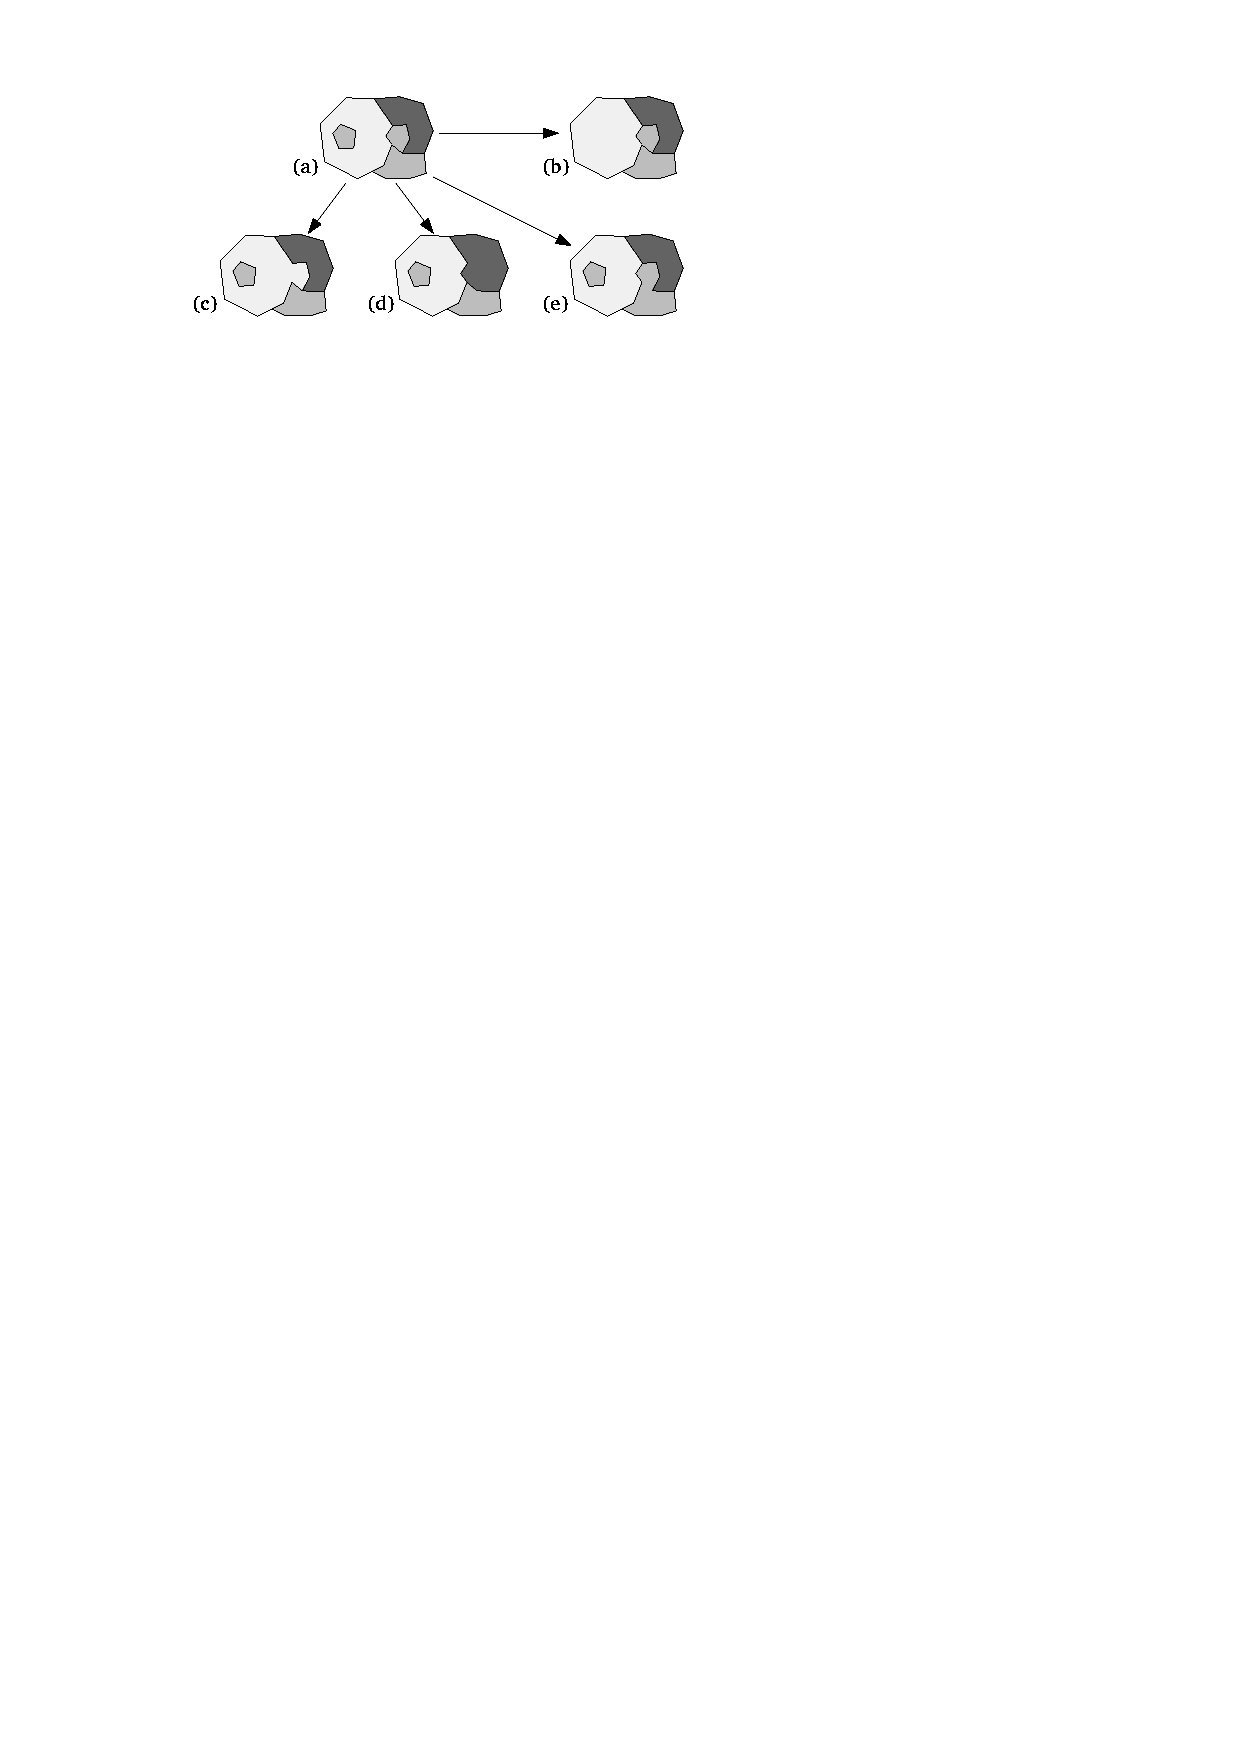
\includegraphics[page=1]{AreaAgg_CostsAndEstimations}
\caption{Aggregating land-cover areas 
	according to different preferences
    by \textcite{Cheng2006}.
	Aggregating a small land-cover area into another one 
	that isolates the area (b), 
	that is the largest neighbor (c), 
	that shares the longest boundary (d), or 
	that has the most similar type (e).}
\label{fig:AreaAgg_Preferences}	
\end{figure}


\subsection{Cost of Type Change}
\label{sec:AreaAgg_f_type}

Suppose that we are at the step of aggregating 
from subdivision~$P_{s,i}$ to subdivision~$P_{s+1,j}$. 
In this step, patch~$u$ is aggregated into patch~$v$
(see \figs\ref{fig:AreaAgg_FirstStep}a 
and \ref{fig:AreaAgg_FirstStep}b).
We denote the types of the two patches by~$T(u)$ and~$T(v)$. 
We define the cost of type change of this step by
\begin{equation}
\label{eq:f_type}
f_\mathrm{type}(P_{s,i},P_{s+1,j})=\frac{A_{u}}{A_R}
\cdot
\frac{d_\mathrm{type}(T(u),T(v))}{d_\mathrm{type\_max}},
\end{equation}
where~$A_u$ is the area of patch~$u$, 
and~$A_R$ is the area of region~$R$
(see \sect\ref{sec:AreaAgg_Preliminaries}).
We use~$A_R$ and~$d_\mathrm{type\_max}$ 
to normalize the cost of type change. 
Constant~$d_\mathrm{type\_max}$, the maximum cost over all type changes,  
is known from the input. 
The input specifies
cost~$d_\mathrm{type}(T_1,T_2)$ of changing type~$T_1$ to type~$T_2$.
Specifically, we denote by~$T_\mathrm{goal}$ the type of 
the patch on the goal map.
For simplicity, we use a metric 
as the cost function of type change
(see \sect\ref{sec:AreaAgg_CaseStudy}).
A metric distance is symmetric, 
which is different from the asymmetric one used in
\textcite{Dilo2009tGAP}.
In their definition, for example, 
the distance from type \emph{building} to type \emph{road} is~$0.5$,
but the distance from \emph{road} to \emph{building} is~$0$.

For path $\Pistar=(P_{1,i_1}, P_{2,i_2}, \dots, 
P_{\tstar,i_{\tstar}})$,
we define the cost of type change over the steps 
by
\begin{equation}
\label{eq:g_type}
g_\mathrm{type}(\Pistar)=
\sum_{s=1}^{t-1}f_\mathrm{type}(P_{s,i_s},P_{s+1,i_{s+1}}).
\end{equation}

\begin{figure}[tb]
\centering
\includegraphics[page=2]{AreaAgg_CostsAndEstimations}
\caption{An aggregation step, 
	where patch~$u$	is aggregated into patch~$v$; 
    see \figs(a) and~(b).
	\figs(c) and~(d) respectively show the number of 
	edges and the lengths of the interior polylines after 
	the aggregation.}
\label{fig:AreaAgg_FirstStep}	
\end{figure}

\subsection{Cost of Compactness}
\label{sec:AreaAgg_f_comp}

We use the compactness definition of \citet{Frolov1975}, 
i.e., the compactness value of a patch, say,~$u$ is
\begin{equation}
\label{eq:comp}
c(u)=\frac{2 \sqrt{\pi A_u}}{l_u},
\end{equation}
where~$A_u$ and~$l_u$ are 
the area and the perimeter. 
For subdivision \Psnode, we denote by~$C(\Psnode)$ 
the set of the patches' compactness values.

We wish to maximize the sum of the average compactness values 
over all intermediate maps,
while our objective will be
minimizing a cost function.
To adapt the average compactness to our methods, 
we define and minimize a cost related to compactness.
Recalling that there are~$n-s+1$ patches at time~$s$,
we define the cost of compactness for subdivision~\Psnode as
\begin{equation}
\label{eq:f_comp}
f_\mathrm{comp}(\Psnode)=
\frac{1-\frac{1}{n-s+1} \sum_{c\in C(\Psnode)}c}{n-2},
\end{equation}
where we use values~$n-s+1$ and~$n-2$ to normalize 
the cost of compactness.

For path $\Pistar$ (see \sect\ref{sec:AreaAgg_f_type}),  
we define the cost of compactness over all 
intermediate maps
(that is, neglecting~$P_{1,1}$ 
and the last subdivision in the path) by
\begin{equation}
\label{eq:g_comp}
g_\mathrm{comp}(\Pistar)=
\sum_{s=2}^{\tstar-1}f_{\mathrm{comp}}(P_{s,i_s}).
\end{equation}


\subsection{Cost of Length}
\label{sec:AreaAgg_costlength}

We denote the set of interior boundaries 
for a subdivision~$\Psnode$ by~$B(\Psnode)$.
The cost in terms of interior length of 
this subdivision is defined as
\begin{equation}
\label{eq:f_length}
f_\mathrm{lgth}(\Psnode)=
\frac{\big(\sum_{b\in B (\Psnode)} 
	|b|\big)\big/D(s)}{n-2}, 
\end{equation} 
where 
\begin{equation}
\label{eq:AreaAgg_Norm}
D(s)=\frac{n-s}{n-1} \sum_{b\in B (\Pstart)} |b|.
\end{equation}
Function~$D(s)$ computes the ``expected'' total length of 
the interior boundaries at time~$s$,
where we expect that this total length decreases linearly
according to time~$s$.
In special,~$D(1) = \sum_{b\in B (\Pstart)} |b|$
and~$D(n) = 0$.
Similarly to \eq\ref{eq:f_comp}, 
we use~$D(s)$ and~$n-2$ to normalize 
the cost of length.


For path~$\Pistar$ (see \sect\ref{sec:AreaAgg_f_type}), 
we define the cost of length over all 
intermediate maps 
(that is, neglecting~$P_{1,1}$ 
and the last subdivision in the path) by
\begin{equation}
\label{eq:g_length}
g_\mathrm{lgth}(\Pistar)=
\sum_{s=2}^{\tstar-1}f_{\mathrm{lgth}}(P_{s,i_s}).
\end{equation}

Note that in theory, a patch, $u$, with a small perimeter 
can be extremely non-compact 
according to measure~$c(u)$ in \eq\ref{eq:comp}, 
thus the two measures, $f_\mathrm{comp}$ and~$f_\mathrm{lgth}$, 
are not interchangeable. 
However, if we assume that all areas of the map have the same size 
(i.e., $A_u$ of \eq\ref{eq:comp} is a constant), 
it would make no difference whether 
we minimize an area's perimeter 
or maximize the area's compactness~$c(u)$. 
Obviously, the areas in our dataset have different sizes. 
However, since we iteratively remove the smallest area, 
the differences do not become too large. 
Therefore, measuring the overall compactness of a map 
based on the total length of 
all the interior boundaries is quite reasonable.

\subsection{Combining Cost Functions}
\label{sec:AreaAgg_Combining}
When we generate a sequence of intermediate-scale maps,
we want to change the types of the land-cover areas 
as little as possible
and want to have compact land-cover areas.
Therefore, we combine 
the cost of type change (\eq\ref{eq:g_type})
and the cost of compactness (\eq\ref{eq:g_comp}).
That is,
\begin{equation}
\label{eq:g_1}
g_1(\Pistar)= (1-\lambda)g_\mathrm{type}(\Pistar)
+\lambda g_\mathrm{comp}(\Pistar),
\end{equation}
where~$\lambda \in [0,1]$ is a parameter 
to assign importances 
of~$f_\mathrm{type}$ and~$f_\mathrm{comp}$.
We simply use~$\lambda=0.5$ in our experiments. 
We want to find a path~$\Pi$ from~$\Pstart$ to~$\Pnode$ 
that minimizes, among all such paths,~$g_1(\Pistar)$.
Slightly abusing notation, we denote the cost of
an optimal path from~${P}_{\mathrm{start}}$ to~\Pnode 
by~$g_1(\Pnode)$.
Using $g_1(\Pnode)$, we compare a greedy algorithm and \Astar
in finding optimal sequences for area aggregation.

As said before, we want to make a comparison involving
integer linear programming 
while our cost of compactness (see \eq\ref{eq:comp})
cannot be computed linearly in an integer linear program.
Therefore, we combine 
the cost of type change (\eq\ref{eq:g_type})
and the cost of length (\eq\ref{eq:g_length}),
which can be computed linearly in an integer linear program. 
That is,
\begin{equation}
\label{eq:g_2}
g_2(\Pistar)= (1-\lambda)g_\mathrm{type}(\Pistar)
+\lambda g_\mathrm{lgth}(\Pistar).
\end{equation}
We compare the greedy algorithm, \Astar, and an ILP-based 
algorithm using~$g_2$.

\section{NP-hardness Proof}
\label{sec:AreaAgg_NP-hardness}

Although we have shown that the graph of subdivisions
has an exponential size
(see \sect\ref{sec:AreaAgg_Preliminaries}),
one may develop a clever algorithm 
to find an optimal sequence efficiently.
In the following, we prove that 
finding such a sequence is indeed NP-hard.
In the proof, we neglect the cost of compactness or the cost of length.
Considering one of the two costs 
will make the computation even more difficult.


\newtheorem{thm}{Theorem}
\begin{thm}
\textsc{AreaAggregationSequence} is NP-hard 
even if we only consider the cost of type change.
\end{thm}

\begin{proof}
Our NP-hardness proof is by reduction from 
the NP-complete problem \textsc{PlanarVertexCover}, 
which is to decide, for a given 
planar graph~$G_\mathrm{A} = (V_\mathrm{A},E_\mathrm{A})$, 
whether there exists a vertex cover 
with at most a given number~$k_\mathrm{A}$ of vertices. 
For an instance of \textsc{PlanarVertexCover}
(\fig\ref{fig:AreaAgg_Reduction}a), 
we define a corresponding instance of \textsc{AreaAggregationSequence}
whose start map consists of gray, black, and white areas and 
whose goal map consists of only one large gray patch.
The adjacency graphs of the two maps are illustrated 
in \figs\ref{fig:AreaAgg_Reduction}b and~\ref{fig:AreaAgg_Reduction}c, 
where the colors of the vertices represent 
the colors of the corresponding areas.
More precisely, for each vertex of~$G_\mathrm{A}$
in \fig\ref{fig:AreaAgg_Reduction}a, 
we define a gray vertex and a black vertex, 
which we connect with an edge. 
For each edge $\{u,v\}$ of~$G_\mathrm{A}$, 
we define two white vertices and 
connect each of them both with the black vertex for~$u$
and the black vertex for~$v$
(\fig\ref{fig:AreaAgg_Reduction}b).

\begin{figure}[tb]
\centering
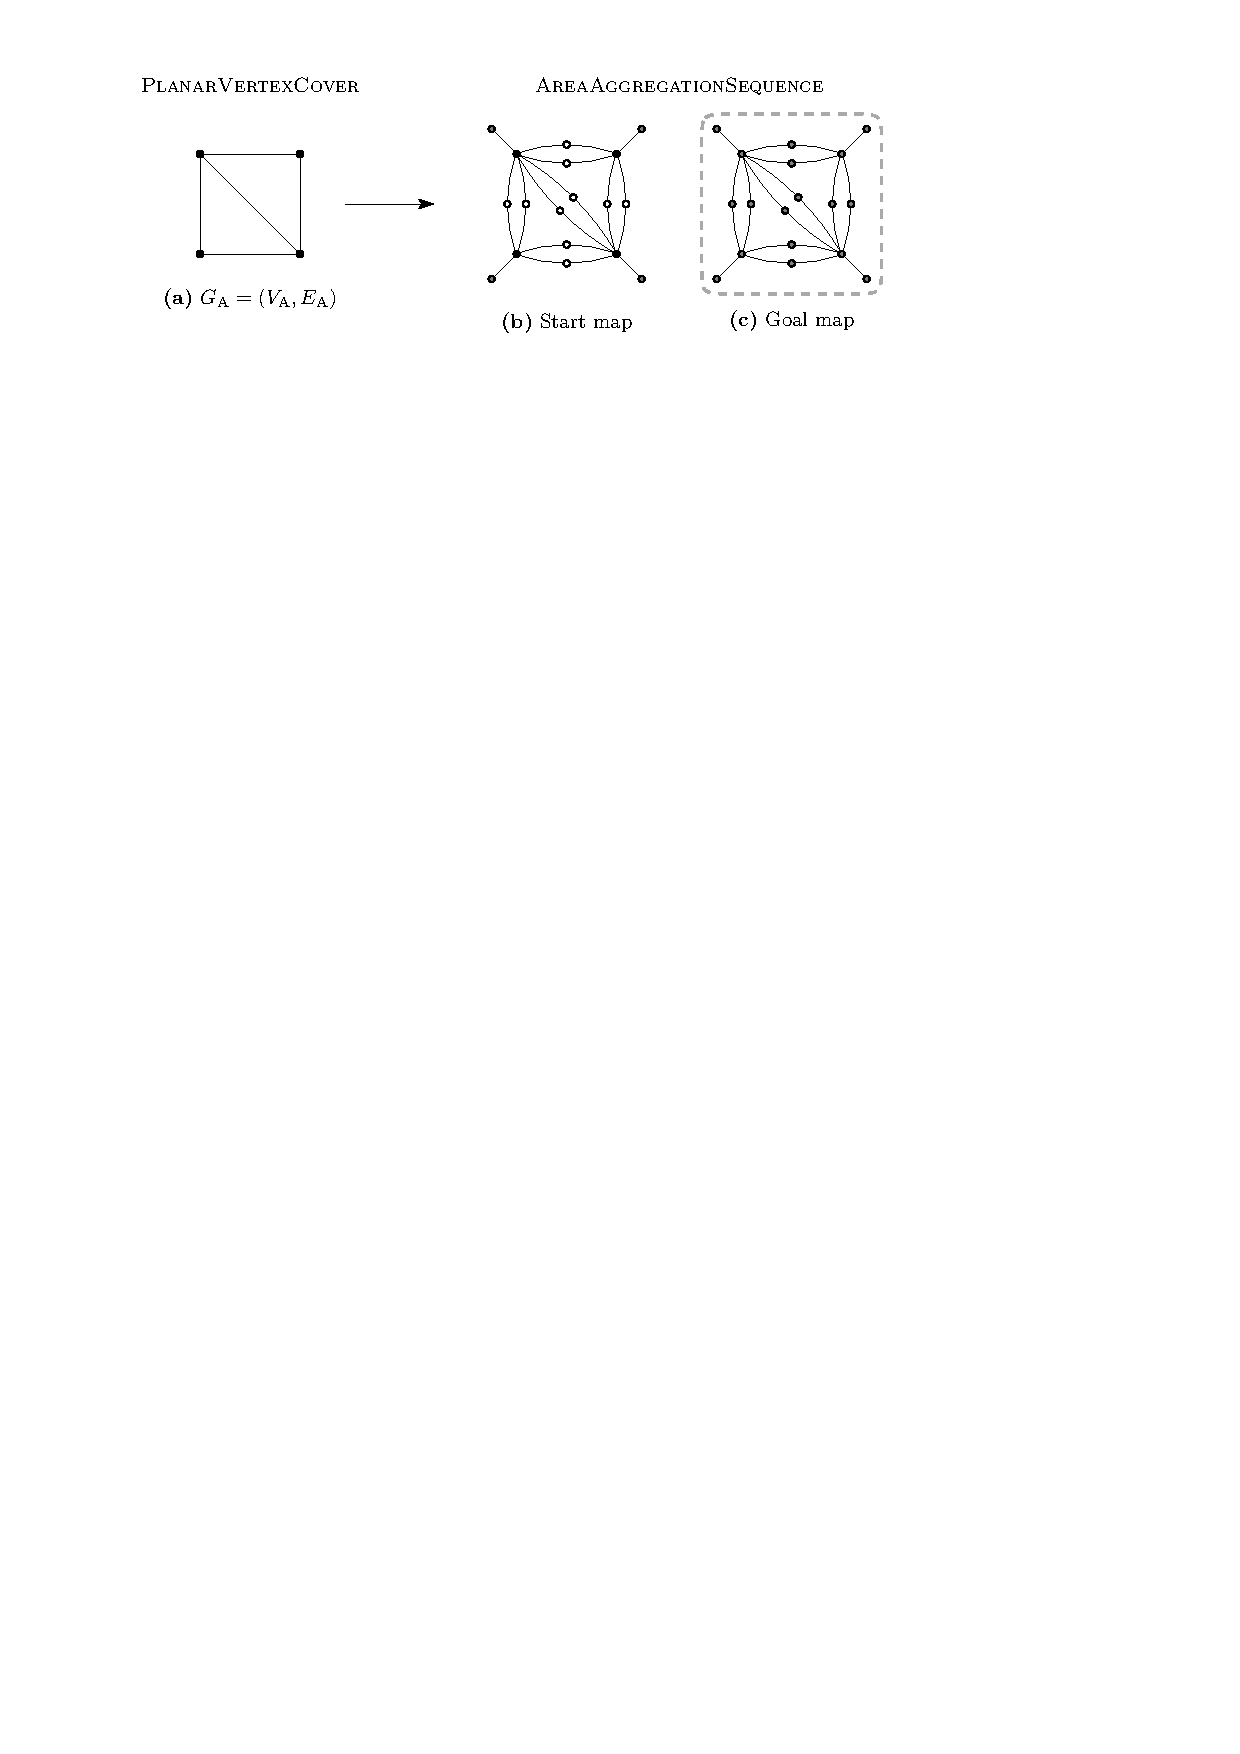
\includegraphics[page=1]{AreaAgg_NPHard}
\caption{The reduction for our NP-hardness proof.
    The dashed polygon in (c) shows 
    the merged vertices.}
\label{fig:AreaAgg_Reduction}
\end{figure}

We define the weights of the vertices 
in \fig\ref{fig:AreaAgg_Reduction}b as follows:
\begin{itemize}[noitemsep,topsep=0pt,parsep=0pt,partopsep=0pt]
\item Every white vertex has weight~$1$.
\item Every black vertex has weight~$2$.
\item Every gray vertex has weight~$2|V_\mathrm{A}| + 2|E_\mathrm{A}|$,
which is equal to the total weight of all white and black vertices.
\end{itemize}
When we merge two vertices, 
the weight of the new vertex is the sum of the two.
In each aggregation step, 
we require the smallest area to be aggregated with one of its neighbors.
The area sizes correspond to the weights of the vertices in \fig\ref{fig:AreaAgg_Reduction}b.   
Therefore, our definition of the weights to a certain degree determines 
the order in which the vertices are selected:
\begin{itemize}[noitemsep,topsep=0pt,parsep=0pt,partopsep=0pt]
\item \emph{Phase I}: In each of the first~$2|E_\mathrm{A}|$ steps, 
a white vertex is selected and merged with one of its neighbors, 
such that the white vertex receives the neighbor's color or vice versa
(\fig\ref{fig:reduction2} shows a possible result).
\item \emph{Phase II}: In each of the next~$|V_\mathrm{A}|$ steps, 
a non-gray vertex is selected and merged with one of its neighbors.
\item \emph{Phase III}: $|V_\mathrm{A}|-1$ steps remain to reach the goal map.
\end{itemize}

To complete the reduction, 
we need to define the costs of color changes. 
For any color change, 
we charge one unit of cost per unit weight.
Due to our construction, Phases II and III can be accomplished with
a total cost of~$2|V_\mathrm{A}|+2|E_\mathrm{A}|$, 
no matter how Phase I is accomplished.
This is because, after Phase I, 
every non-gray patch will be adjacent to a gray patch (vertex).
Thus, if any non-gray patch becomes selected in Phase II, 
it can be aggregated with a gray patch (vertex) and 
receive the color gray. 
This implies that Phase II costs $2|V_\mathrm{A}|+2|E_\mathrm{A}|$ 
(which is equal to the total weight of 
all initially white and black vertices) and, 
since after Phase II all patches are gray, 
Phase III does not cause any additional cost.  
It is also clear that 
there is no cheaper way to accomplish Phases II and III,
since it is impossible to color a vertex gray in Phase I.
Consequently, since the total cost of Phases II and III is fixed, 
it is only interesting to ask 
at which cost Phase I can be accomplished.
It turns out that, if $G_\mathrm{A}$ 
has a vertex cover $C_\mathrm{A} \subseteq V_\mathrm{A}$, 
then Phase I can be accomplished with cost $2|C_\mathrm{A}|$;
only the black vertices corresponding to vertices in~$C_\mathrm{A}$ 
need to change their color from black to white, and 
each of them has weight~$2$ (see \fig\ref{fig:reduction2}).
To summarize, if graph~$G_\mathrm{A}$ has a vertex cover~$C_\mathrm{A}$, 
then the corresponding instance of \textsc{AreaAggregationSequence} 
has a solution of 
total cost~$2|C_\mathrm{A}|+2|V_\mathrm{A}|+2|E_\mathrm{A}|$.

It remains to be shown that, 
if $C_\mathrm{A}^*$ is a minimum vertex cover of $G_\mathrm{A}$, 
then there is no solution with total cost 
less than $2|C_\mathrm{A}^*|+2|V_\mathrm{A}|+2|E_\mathrm{A}|$.
To see why, we assume that such a solution exists.
If we keep the black color of a vertex from $C_\mathrm{A}^*$ 
(the total cost decreases by $2$),
then we will need to at least change two white vertices
to black vertices
(the total cost increases by $2$ at least).
Therefore, we have found a contradiction to our assumption.

\begin{figure}[tb]
\centering
\includegraphics[page=2]{AreaAgg_NPHard}
\caption{The situation after Phase I has been conducted 
    such that all black vertices corresponding to a vertex cover 
    of~$G_\mathrm{A}$ have been recolored white.
    The dashed polygons show that the vertices are merged.}
\label{fig:reduction2}
\end{figure}
\end{proof}

\section{A Greedy Algorithm}
\label{sec:AreaAgg_Greedy}

A motivation for the greedy algorithm is that 
a very similar iterative algorithm has been used by
\textcite{vanOosterom2005} 
for constructing the tGAP data structure.
However, we have to make minor modifications to ensure that 
the computed aggregation sequence ends with the goal map that, 
in our situation, is given as a part of the input.
We use our greedy algorithm as a benchmark
so that we are able to see 
whether the \Astar algorithm or the ILP-based algorithm 
indeed perform better.

At any time~$t$,
our greedy algorithm aggregates the smallest patch
with one of its neighbors.
We pick the neighbor in a greedy way.
We suppose that the smallest patch,~$u$, has~$k_u$ neighbors,
then there are~$2k_u$ ways to aggregate
(when we aggregate a patch into another patch,
the union uses the type of the latter).
In order to guarantee that our final result
(e.g., the polygon of layer~$L_4$ in 
\fig\ref{fig:AreaAgg_SubdivisionName})
will have the type of~$T_\mathrm{goal}$,
we add one more rule to our greedy algorithm.
Suppose that patch~$v$ is one of~$u$'s neighbors.
The greedy algorithm aggregates~$u$ into~$v$ 
if the type distances fulfill that
$d_\mathrm{type}\left(T(u), T_\mathrm{goal}\right) 
\ge d_\mathrm{type}\left(T(v), T_\mathrm{goal}\right)$;
otherwise, the algorithm aggregates~$v$ into~$u$.
This rule excludes, say,~$k_e$ aggregation choices,
and we have~$2k_u - k_e$ choices left.
Then we compute the costs for each of 
the~$2k_u - k_e$ aggregation choices
and select the aggregation that has the least cost.
In other words, we aggregate the smallest patch with 
its most \emph{compatible} neighbor.

In accordance with our two combinatorial costs in 
\sect\ref{sec:AreaAgg_Combining},
we define two cost functions.
Suppose that we are at the step of aggregating 
from subdivision~$P_{s,i}$ to subdivision~$P_{s+1,j}$.
The first cost function is 
\begin{equation}
\label{eq:f_1}
f_1(P_{s,i},P_{s+1,j})=
(1-\lambda)f_\mathrm{type}(P_{s,i},P_{s+1,j})
+\lambda f_{\mathrm{comp}}(P_{s+1,j}).
\end{equation}
The second cost function is
\begin{equation}
\label{eq:f_2}
f_2(P_{s,i},P_{s+1,j})=
(1-\lambda)f_\mathrm{type}(P_{s,i},P_{s+1,j})
+\lambda f_{\mathrm{lgth}}(P_{s+1,j}).
\end{equation}
We take one of the~$2k_u - k_e$ aggregation choices 
according to \eqs\ref{eq:f_1} or~\ref{eq:f_2}
in our two experiments.
The cost of a whole sequence can be computed by
\eqs\ref{eq:g_1} or~\ref{eq:g_2}.







\section{Using the \texorpdfstring{\Astar Algorithm}{A* Algorithm}}
\label{sec:AreaAgg_AStar}

\sect\ref{sec:AreaAgg_Preliminaries} has shown that
the size of finding an optimal aggregation sequence 
can be exponential.
That is to say, the graph~$G_\mathrm{S}$---our search space---can 
be of exponential size.
In order to avoid computing the whole graph explicitly,
we use the \Astar algorithm \parencite{Hart1968,PatelAStar}.
To save time and memory, 
we generate a subdivision, \Pnode, only 
when we are going to visit it.
\Astar uses a clever best-first search 
to find a shortest path 
from subdivision~$\Pstart$ to subdivision~$\Pgoal$.  
For \Pnode,
\Astar considers the exact cost of a shortest path 
from~\Pstart to~\Pnode 
and estimates the cost to get from~\Pnode to~\Pgoal. 
\Astar explores the nodes earlier 
if they are estimated to be closer to the goal.
\Astar can be seen as a refinement of Dijkstra's algorithm
\parencite{Dijkstra1959}.

We define~$g(\Pnode)$ to be 
the exact cost of a shortest path from~\Pstart to~\Pnode 
and define~$h(\Pnode)$ to be the estimated cost 
to get from \Pnode to~\Pgoal. 
Then, the (estimated) total cost at node~\Pnode is
\begin{equation}
\label{eq:CostTotal}
F(\Pnode)=g(\Pnode)+h(\Pnode).
\end{equation}
We use either~$g_1$ (\eq\ref{eq:g_1}) 
or~$g_2$ (\eq\ref{eq:g_2}) for~$g(\Pnode)$;
accordingly, we use either~$h_1$ (\eq\ref{eq:h_1}) 
or~$h_2$ (\eq\ref{eq:h_2}) for~$h(\Pnode)$.
If~$h(\Pnode)$ is always bounded from above 
by the exact cost of a shortest path from~\Pnode to~\Pgoal, 
\Astar guarantees to find a shortest path from~\Pstart 
to~\Pgoal, 
that is, an optimal aggregation sequence.  
Using estimate~$F$ (\eq\ref{eq:CostTotal}), 
\Astar is able to reduce the search space.
The better the estimation part~$h$, 
the more search space \Astar can reduce.
In the following, we show how to compute
estimated cost~$h(\Pnode)$.

To narrow down the search space, 
we set up estimation functions 
for type change (\sect\ref{sec:AreaAgg_h_type}), 
compactness (\sect\ref{sec:AreaAgg_h_comp}), 
and length (\sect\ref{sec:AreaAgg_h_length}). 
These functions are meant to direct \Astar towards the goal.
Since the number of subdivisions can be exponential, 
we may run out of the main memory 
before we find an optimal solution. 
To handle this problem, we introduce overestimations 
to find a feasible solution. 
Overestimations are popular 
when people cannot find optimal solutions using \Astar. 
For example, \textcite{Pohl1973} overestimated 
using dynamic weighting. 
We propose another strategy that fits our problem. 
We first try finding an optimal solution by \Astar. 
If we fail to find one after 
we have visited a predefined number, 
say,~$W$ of nodes of graph~$G_\mathrm{S}$,
then we restart.
In the retrying, we overestimate the first~$K$ steps 
starting at each node
(see \sects\ref{sec:AreaAgg_h_type}, \ref{sec:AreaAgg_h_comp},
and~\ref{sec:AreaAgg_h_length}).
We may need to increase~$K$ and retry several times 
until we find a feasible solution.
Because we do not want to retry too many times,
we define~$K$ by
\begin{equation}
\label{eq:OverestimateK}
K= 2^k -1,
\end{equation}
where~$k\ge 0$ is the number of retryings.
When~$k = 0$, we have~$K=0$,
which means that the first attempt of finding a solution
does not use overestimation.
As~$K\le n-1$, it holds that~$k \le \log_2 n$, 
which means that we need to 
retry~$\lceil \log_2 n\rceil$ times at most.
Whenever overestimating ($k\geq1$), 
\Astar cannot guarantee optimality anymore.
When we are at time~$t$, there are at most~$n-t$ steps 
to arrive at the goal map.
We define the number of practical overestimation steps as
\begin{equation}
\label{eq:OverestimateKPrime}
K'= \min \{K, n-t\}.
\end{equation}



\subsection{Estimating the Cost of Type Change}
\label{sec:AreaAgg_h_type}

To find a lower bound of the cost of type change, 
we simply assume that 
every patch will be aggregated into a patch with type~\Tgoal.
As long as the cost of type change is a metric, this aggregation 
strategy indeed yields a lower bound.
%
For subdivision~\Pnode, let
$(\Pnode=P_{t,i'_t}, P_{t+1,i'_{\tstar+1}} \dots,P_{n,i'_n}=\Pgoal)$,
be the path that always changes the type of a smallest patch 
to~\Tgoal.
Then the estimated cost of type change is
\begin{equation}
\label{eq:h_type}
h_\mathrm{type}(\Pnode)=
\sum_{s=t}^{n-1}f_\mathrm{type}(P_{s,i'_s},P_{s+1,i'_{s+1}}).
\end{equation}

As an example, for \fig\ref{fig:AreaAgg_FirstStep}b, we compute 
$h_\mathrm{type}$ 
according to the ``aggregation sequence'' of 
\fig\ref{fig:AreaAgg_h_type}.
Note that the step from
subdivision~$P_{2,i'_2}$ to subdivision~$P_{3,i'_3}$ 
in \fig\ref{fig:AreaAgg_h_type} is impossible in reality 
because the dark patch cannot be aggregated into patch~$v$
as they are not neighbors. 
However, this aggregation is allowed for estimation 
because we may find a shortest path as long as 
the estimated cost is no more than 
the exact cost of a shortest path.
When we need to overestimate, we multiply the estimated cost of the 
first~$K'$ steps (see \eq\ref{eq:OverestimateKPrime}) 
by~$K$ (see \eq\ref{eq:OverestimateK}).
As a result, \fo\ref{eq:h_type} is revised to
\begin{equation}
\label{eq:o_type}
h_\mathrm{type}(\Pnode)=
K\sum_{s=t}^{t+K'-1}f_\mathrm{type}(P_{s,i'_s},P_{s+1,i'_{s+1}})+
\sum_{s=t+K'}^{n-1}f_\mathrm{type}(P_{s,i'_s},P_{s+1,i'_{s+1}}).
\end{equation}


\begin{figure*}[tb]
\centering
\includegraphics[page=3]{AreaAgg_CostsAndEstimations}
\caption{An ``aggregation sequence'' for computing
    the estimated cost of type change~$h_{\mathrm{type}}$
    (see \eqs\ref{eq:h_type} and~\ref{eq:o_type}),
	based on the aggregation result of 
	\fig\ref{fig:AreaAgg_FirstStep}b.
    Note that this aggregation sequence is impossible in reality,
    but it is fine for estimating
    (see the argument in \sect\ref{sec:AreaAgg_h_type}).}
\label{fig:AreaAgg_h_type}
\end{figure*}


\subsection{Estimating the Cost of Compactness}
\label{sec:AreaAgg_h_comp}

We estimate the cost of compactness based on regular polygons.
The more edges a regular polygon has, the more compact it is.
We assume that, at each step, 
we aggregate the two patches that are the least compact.
Moreover, we assume that the shared boundary of the two patches  
has the least number of edges.
We use $\mathcal{N}_\mathrm{ext}$ to 
denote the edge number of the region's exterior boundaries.
As the exterior boundaries will not be changed by aggregation, 
$\mathcal{N}_\mathrm{ext}$ 
is a constant. 
%
Note that the boundary between two patches 
is not necessarily connected; 
for example, see the dark boundary with three edges 
in \fig\ref{fig:AreaAgg_h_comp}a.
For subdivision \Pnode,
we denote by~$B(\Pnode)$ the set of interior boundaries 
and denote by~$b_\mathrm{min}(\Pnode)$ 
the boundary with the smallest number of edges.
For our estimation, the set of interior boundaries 
at time~$t+1$ 
is~$B(P_{t+1,i''_{t+1}})= B(\Pnode)-{\{b_\mathrm{min}(\Pnode)\}}$. 
The estimated number of the edges for 
such a subdivision,~$P_{t+1,i''_{t+1}}$, is
\begin{equation}
\label{eq:LeftEdgeNum}
\mathcal{N}_{t+1,i''_{t+1}}=
\mathcal{N}_\mathrm{ext} + \sum_{b \in B(P_{t+1,i''_{t+1}})} \|b\|,
\end{equation}
where notation~$\|b\|$ represents the number of boundary~$b$'s edges.

\begin{figure*}[tb]
\centering
\includegraphics[page=4]{AreaAgg_CostsAndEstimations}
\captionof{figure}{An "aggregation sequence" for 
	computing the estimated cost of compactness~$h_\mathrm{comp}$ 
    (see \eqs\ref{eq:h_comp} and~\ref{eq:o_comp}), 
    based on the number of edges. 
	At each step we remove the boundary with the fewest edges. 		
	The numbers represent the 
	numbers of the interior boundaries' edges.
    Note that this aggregation sequence is impossible in reality,
    but it is fine for estimating
    (see the argument in \sect\ref{sec:AreaAgg_h_type}).    
	This example corresponds to the aggregation step in 
	\fig\ref{fig:AreaAgg_FirstStep}b.
}
\label{fig:AreaAgg_h_comp}
\end{figure*}

From subdivision~\Pnode to subdivision~$P_{t+1,i''_{t+1}}$,
we get a new patch because of the aggregation.
The new patch is certainly less compact than a regular polygon 
with~$\mathcal{N}_{t+1,i''_{t+1}}$ edges.
In order to estimate the compactness of the new patch, 
we assume that 
the new patch has the shape of a regular polygon 
with~$\mathcal{N}_{t+1,i''_{t+1}}$ edges 
(see \eq\ref{eq:LeftEdgeNum}).
A regular polygon with~$\mathcal{N}$ edges has compactness
\begin{equation*}
\label{eq:comp_regular}
c_\mathrm{reg}(\mathcal{N})=
\sqrt{\frac{\pi}{\mathcal{N}} \bigg/
	\tan{\frac{\pi}{\mathcal{N}}}}.
\end{equation*}
Note that compactness~$c_\mathrm{reg}(\mathcal{N})$ increases  
with increasing~$\mathcal{N}$.
A patch with~$\mathcal{N}_{t+1,i''_{t+1}}$ edges has
compactness~$c_\mathrm{reg} (\mathcal{N}_{t+1,i''_{t+1}})$.
According to our previous assumption, 
at each step we are always able to aggregate the two patches 
that are the least compact in the subdivision.
We denote the compactness values of the two patches
by~$c_\mathrm{min1}(\Pnode)$ and~$c_\mathrm{min2}(\Pnode)$.
Recall that we use~$C(\Pnode)$ to denote 
the set of compactness values of the patches
in subdivision~$\Pnode$ 
(see \sect\ref{sec:AreaAgg_f_comp}).
Then the set of compactness values 
for subdivision~$P_{t+1,i''_{t+1}}$ is 
\begin{equation}
\label{eq:compsetnew}
C(P_{t+1,i''_{t+1}})=
C(\Psnode)\cup 
\{c_\mathrm{reg} (\mathcal{N}_{t+1,i''_{t+1}})\}
\setminus \{c_\mathrm{min1}(\Pnode), c_\mathrm{min2}(\Pnode)\}.
\nonumber
\end{equation}
We compute the estimated average compactness 
by calculating the average 
of the values in set~$C(P_{t+1,i''_{t+1}})$.
Finally, we compute the estimated cost of compactness 
for subdivision~$P_{t+1,i''_{t+1}}$ by \eq\ref{eq:f_comp}.

For subdivision~\Pnode, let
$(\Pnode=P_{t,i''_t}, P_{t+1,i''_{\tstar+1}}, 
\dots,P_{n,i''_n}=\Pgoal)$
be the path that always removes the two smallest compactnesses
and gains a compactness of the constructed regular polygon.
The estimated cost of compactness is
\begin{equation}
\label{eq:h_comp}
h_\mathrm{comp}(\Pnode)=
\sum_{s=t}^{n-1}f_\mathrm{comp}(P_{s,i''_s}).
\end{equation}
When overestimating, we assume that 
each patch in the subdivision is extremely noncompact,
that is, each patch has compactness~$0$.
One may ask if this assumption is too much.
It is indeed too much for one subdivision, 
but it is just fine for the whole sequence
as we overestimate for only a certain number of subdivisions.
Based on the assumption, the cost of compactness 
is~$f_\mathrm{comp}(P_{s,i''_s})=1/(n-2)$,
according to \eq\ref{eq:f_comp}.
When we need to overestimate $K'$ steps
(see \eq\ref{eq:OverestimateKPrime}), 
we revise the estimated cost of compactness to
\begin{equation}
\label{eq:o_comp}
h_\mathrm{comp}(\Pnode)=
\sum_{s=t}^{t+K'-1}\frac{1}{n-2}+
\sum_{s=t+K'}^{n-1}f_\mathrm{comp}(P_{s,i''_s}).
\end{equation}



\subsection{Estimating the Cost of Length}
\label{sec:AreaAgg_h_length}

At time $s$, there are $n-s+1$ patches.
There can be as few as $n-s$ interior boundaries.
In order to find a lower bound for the cost of length,
we keep only the necessary number, $n-s$, 
of shortest boundaries at each step
(see \fig\ref{fig:AreaAgg_h_length}).
Then, we compute the estimated cost of length according to 
\eq\ref{eq:f_length}.

For subdivision~\Pnode, let
$(\Pnode=P_{t,i'''_t}, P_{t+1,i'''_{\tstar+1}}, 
\dots,P_{n,i'''_n}=\Pgoal)$
be the path that always keeps 
the necessary number of shortest interior boundaries.
The estimated cost of length is
\begin{equation}
\label{eq:h_length}
h_\mathrm{lgth}(\Pnode)=
\sum_{s=t}^{n-1}f_\mathrm{lgth}(P_{s,i'''_s}).
\end{equation}
When overestimating,
we use the interior length of subdivision~\Pnode
as the cost of length for each of the first $K'$ steps 
(see \eq\ref{eq:OverestimateKPrime}),
even though we are removing interior boundaries
step by step.
As a result, we revise \fo\ref{eq:h_length} to
\begin{equation}
\label{eq:o_length}
h_\mathrm{lgth}(\Pnode)=
\sum_{s=t}^{t+K'-1}f_\mathrm{lgth}(P_{t,i})+
\sum_{s=t+K'}^{n-1}f_\mathrm{lgth}(P_{s,i'''_s}).
\end{equation}


\begin{figure*}[tb]
\centering
\includegraphics[page=5]{AreaAgg_CostsAndEstimations}
\caption{An "aggregation sequence" for computing 
	the estimated cost of length~$h_\mathrm{lgth}$ 
	(see \eqs\ref{eq:h_length} and~\ref{eq:o_length}),
	based on the lengths of interior boundaries. 
	At each step, we keep the necessary number 
	of interior boundaries with least lengths in order to find a 
	lower bound of the total length of the interior boundaries, 
	i.e., $\ell_\mathrm{int}(P_{s,i'''_s})$.
	The numbers represent the 
	lengths of the interior boundaries.
    Note that this aggregation sequence is impossible in reality,
    but it is fine for estimating
    (see the argument in \sect\ref{sec:AreaAgg_h_type}).    
	This example corresponds to the aggregation step in 
	\fig\ref{fig:AreaAgg_FirstStep}b.
}
\label{fig:AreaAgg_h_length}
\end{figure*}


\subsection{Combining Estimated Costs}
\label{sec:AreaAgg_CombinationEstimated}
In accordance 
with our two combinatorial costs in 
\sect\ref{sec:AreaAgg_Combining},
we define two estimated-cost functions:
\begin{equation}
\label{eq:h_1}
h_1(\Pnode)=
(1-\lambda)h_\mathrm{type}(\Pnode)
+\lambda h_{\mathrm{comp}}(\Pnode),
\end{equation}
and
\begin{equation}
\label{eq:h_2}
h_2(\Pnode)=
(1-\lambda)h_\mathrm{type}(\Pnode)
+\lambda h_{\mathrm{lgth}}(\Pnode).
\end{equation}



\section{Integer Linear Programming}
\label{sec:AreaAgg_ILP}

\emph{Linear programming} is a method 
to optimize a \emph{linear objective}
subject to a set of \emph{linear constraints}
with some \emph{variables}.
Suppose that we are selling coffee.
We have~$3.5\,$kg of coffee powder and~$10\,$kg of water.
We mix the powder and the water to provide two kinds coffee 
with different intensities in terms of mass:~$40\%$ and~$20\%$.
The profits of them
are respectively~$5\,$\euro~and~$4\,$\euro.
Our aim is to maximize the total profit of selling coffee.
If we offer~$x\,$kg and~$y\,$kg 
of the two kinds of coffee,
then~$x$ and~$y$ are our variables.
Our objective is to
$$
\mathrm{maximize} 	\quad	 5x+4y.
$$
To provide~$x\,$kg of coffee with intensity~$40\%$,
we need to use~$0.4x\,$kg of coffee powder 
and~$0.6x\,$kg of water.
Analogously, we need~$0.2y\,$kg of powder 
and~$0.8y\,$kg of water to produce~$y\,$kg of coffee
with intensity~$20\%$.
As a result, we have four constraints:
\begin{align*}
0.4x+0.2y	&\le 3.5,				\\
0.6x+0.8y 	&\le 10,	\text{~and}			\\
x,y			&\ge 0.
\end{align*}
With the objective and the constraints, 
we have set up a \emph{linear program} (LP).
We observed that 
all the feasible solutions, i.e., pairs of~$(x,y)$,
fall in the gray area of
\fig\ref{fig:AreaAgg_ILPIllustration}a.
Drawing a line with slope~$-\frac{5}{4}$,
we see that every pair of~$(x,y)$ lying on the line
yields the same result for~$5x+4y$, 
the profit we want to maximize.
For example, every pair of~$(x,y)$ lying on the dashed line
in \fig\ref{fig:AreaAgg_ILPIllustration}a 
yields profit~$40\,$\euro.
If we move the dashed line to the upper right,
then we are able to achieve a larger value for~$5x+4y$. 
In order to maximize the profit, 
we move the dashed line to the upper right as much as possible
and, at the same time, make sure that 
it still intersects with the gray area.
Note that if the dashed line 
does not intersect with the gray area,
then there is no feasible pair of~$(x,y)$ 
on the dashed line anymore.
As a result, we get the optimal solution 
when the dashed line hits point~$A$,
where the profit is~$5 \cdot 4 + 4 \cdot 9.5 =58\,$\euro.
\textcite{Karmarkar1984LP}
proved that an LP can be solved in polynomial time.

\begin{figure*}[tb]
\centering
\includegraphics[page=4]{AreaAgg_ILP}
\caption{Examples of linear programming (a)
	and integer linear programming (b).
    In (a), any point in the gray area is a feasible solution;
    in (b), only the gray points are feasible solutions.
}
\label{fig:AreaAgg_ILPIllustration}
\end{figure*}

Now we change our problem a bit.
We wish to sell coffee in jugs,
where each jug contains exactly~$1\,$kg of coffee 
with intensity~$40\%$ or~$20\%$.
Our question becomes how many jugs of each kind of coffee
we should sell in order to maximize the profit.
If we sell the two kinds of coffee 
respectively~$x'$ and~$y'$ jugs,
then the problem becomes:
\begin{alignat*}{3}
&&\text{maximize} 	\quad	&& 5x'+4y' 		&			\\
&&\text{subject to} \quad	&& 0.4x'+0.2y'	&\le 3.5, 	\\
&&					\quad	&& 0.6x'+0.8y' 	&\le 10, 	\\
&&					\quad	&& x', y' 		&\ge 0, 	\\
&&\text{and} 		\quad	&& x', y'		&\in \mathbb{Z}.
\end{alignat*}
For this problem, only the pairs of~$(x',y')$ 
represented by the gray dots of 
\fig\ref{fig:AreaAgg_ILPIllustration}b 
are feasible solutions
(point~$A$ is no longer a feasible solution in this case).
In order to maximize our profit,
we should move the dashed line to the upper right 
as much as possible
and, at the same time, make sure that 
it hits at least one of the gray dots.
To solve such a problem is known as
\emph{integer linear programming},
which is NP-complete.
Despite the fact, there are
mathematical solvers yielding optimal solutions
for some NP-complete problems in reasonable time
\parencite{Haunert2017Label}.
By using these solvers, 
we benefit from every improvement, by their producers,
for the same class of problems
\parencite{Haunert2017Label}.
The general form of an \emph{integer linear program} (ILP) is
\begin{alignat*}{3}
&&\text{maximize} 	\quad&& \bm{C}^\mathrm{T}\bm{X}	&		\\
&&\text{subject to} \quad&& \bm{EX}			&\le \bm{H}, 	\\
&&					\quad&& \bm{X} 			&\ge \bm{0}, 	\\
&&\text{and}		\quad&& \bm{X} 			&\in \mathbb{Z}^I,
\end{alignat*}
where vector~$\bm{X}$ represents integer variables, 
vector~$\bm{C} \in \mathbb{R}^I$, 
vector~$\bm{H} \in \mathbb{R}^J$,
and~$\bm{E}$ is a $(J \times I)$-matrix over the reals.
Furthermore, if we require 
$$
\bm{X} 	\in \{0,1\}^I,
$$
then we have only binary variables for an ILP.
Binary variables are important 
because they occur regularly in optimizations
\parencite[\sect9.2]{bradley1977applied}.
Also, an ILP with general (bounded) integer variables 
can always be translated to an ILP with binary variables
\parencite[\sect2.3]{Williams2009Integer}.
We are going to use binary variables in our ILP
because it is more intuitive 
to model our problem using binary variables
than using other integers.



We want to compare the \Astar algorithm with 
integer linear programming in finding 
optimal sequences for our aggregation problem. 
Since integer linear programming
can handle only linear constraints, 
we define the compactness of a subdivision as 
the length of the subdivision's interior boundaries.
That is, we use cost function~$g_2$ (see \eq\ref{eq:g_2}).
Our basic idea is to formalize the problem of 
finding a shortest path as an ILP.
Then we solve this ILP by minimizing the total cost.
We define the \emph{center} of a patch as the polygon 
to which other polygons in the same patch are assigned. 
At the beginning, every patch consists of only one polygon, 
and this polygon is the center of the patch.
When we aggregate patch~$u$ into patch~$v$, 
all the polygons of~$u$ are assigned to the center of~$v$,
and the type of~$u$'s polygons 
are changed to the type of $v$'s center.
In the following, we show how to formalize our problem 
as an ILP.
For simplicity, we sometimes denote by \emph{patch~$r$} the 
patch using polygon~$r$ as the center at time~$t$.


\subsection{Variables}
\label{sub:AreaAgg_variables}

Our problem is to decide centers for polygons to be assigned.
Each question of type 
``Is polygon~$p$ assigned to center~$r$?''
can be answered with ``yes'' or ``no''.
Hence, we use binary ($0$--$1$) variables.
We need five sets of variables
in order to formulate our pathfinding problem as an ILP.
%
Recall that We use~$T=\{1,2,\dots,n\}$ to represent the set of times
and use~$P$ to denote the set of $n$ polygons on the start map
(see \sect\ref{sec:AreaAgg_Preliminaries}).
%
The first set of variables is used to tell the program 
our rules for area aggregation.
\begin{figure*}[tb]
\centering
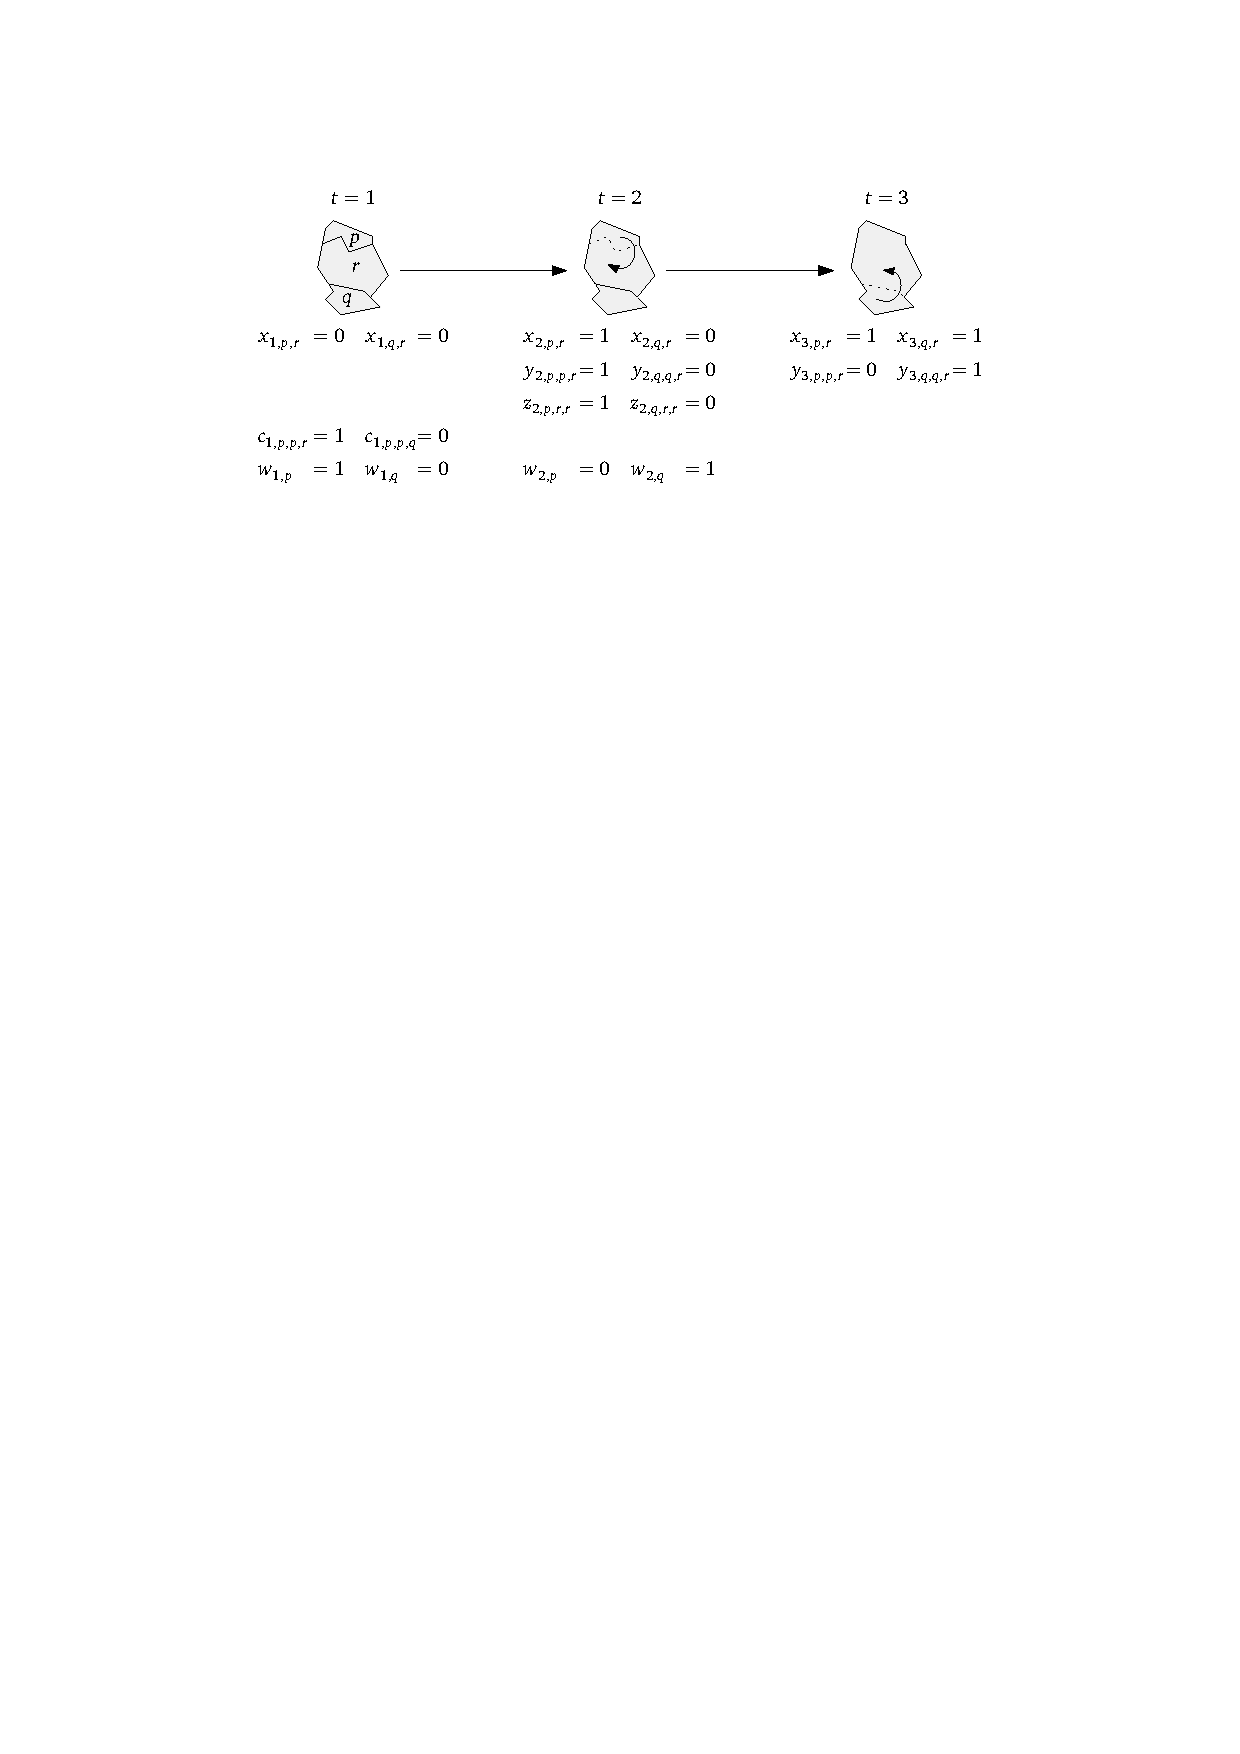
\includegraphics[page=1]{AreaAgg_ILP}
\caption{Some examples of the five sets of variables 
	for our ILP, $x$, $y$, $z$, $c$, and~$w$.
	The arrows with curly arms show the aggregation steps,
    and the dotted lines represent 
	the removed boundaries by the aggregation steps.
	There are some blank spaces in the rows of the variables
    because there is no corresponding variable at the specific times.
}
\label{fig:AreaAgg_Variables}
\end{figure*}
We introduce the variable 
\begin{flalign*}
&\eqquadVariable
\embrd[V]{x_{t,p,r}} \in
\embld[U]{\{0,1\}} \qquad 
\forall t\in T, \forall p,r \in P&
\end{flalign*}
with the intended meaning~$x_{t,p,r}=1$ if and only if 
polygon $p$ is assigned to polygon $r$ at time $t$
(see \fig\ref{fig:AreaAgg_Variables} for some examples). 
If a polygon is a center at time~$t$, 
then the polygon must be assigned to itself, 
that is, $x_{t,r,r}=1$.


We use the second set of variables in order to compute the
cost of type change. We introduce
\begin{flalign*}
&\eqquadVariable
\embrd[V]{y_{t,p,o,r}} \in
\embld[U]{\{0,1\}} \qquad 
\forall t\in T\setminus \{1\}, \forall p,o,r \in P&
\end{flalign*}
with the intended meaning~$y_{t,p,o,r}=1$ if and only if 
polygon~$p$ is assigned to center~$o$ at time~$t-1$ 
and assigned to center~$r$ at time~$t$ 
(see \fig\ref{fig:AreaAgg_Variables}).
Specifically, case~$y_{t,p,o,o}=1$ means that
polygon~$p$ is assigned to the same center 
at times~$t-1$ and~$t$.

We need a third set of variables 
for computing the cost of length.
We introduce
\begin{flalign*}
&\eqquadVariable
\embrd[V]{z_{t,p,q,r}} \in
\embld[U]{\{0,1\}} \qquad 
\forall t\in T\setminus \{1,n\}, \forall p,q,r \in P&
\end{flalign*}
with the intended meaning~$z_{t,p,q,r}=1$ 
if and only if polygons~$p$ and~$q$ 
are both assigned to center~$r$ at time~$t$
($p$ and $q$ are in the same patch).
In this case, their common boundary should be removed
(see \fig\ref{fig:AreaAgg_Variables}).
When variable~$z_{t,p,q,r}=1$ and~$p=q$,
we define the length of their common boundary to be~$0$ 
because we shall not remove any.
Note that time $t\in T\setminus \{1,n\}$.
We do not need~$z_{t,p,q,r}$ for time~$t=1$ 
because there are no two polygons in the same patch.
Namely, it always holds~$z_{1,p,q,r}=0$, 
which does not help in our ILP.
We do not need~$z_{t,p,q,r}$ for time~$t=n$
because all the polygons will be in the same patch.
In this case, \eq$z_{n,p,q,r}=1$ always holds,
which does not help in our ILP, either.

We use a fourth set of variables
to guarantee contiguity of each patch. 
In other words, we aggregate two patches 
only when they are neighbors (adjacent).
We introduce
\begin{flalign*}
&\eqquadVariable
\embrd[V]{c_{t,p,o,r}} \in
\embld[U]{\{0,1\}} \qquad 
\forall t\in T\setminus \{n-1,n\}, 
\forall p,o,r \in P \text{~with}~o\ne r,&
\end{flalign*}
with the intended meaning~$c_{t,p,o,r}=1$ 
if and only if, at time~$t$,
polygon~$p$ is assigned to center~$o$, 
and~$p$ has a neighbor assigned to center~$r$
(see \figs\ref{fig:AreaAgg_Variables}
and~\ref{fig:AreaAgg_Variables_Neighbor} for examples).
We do not need variable~$c_{t,p,o,r}$ for time~$t=n-1$ 
because there are only two patches left, 
and they must be neighbors.

Our last set of variables is needed to 
enforce that
every aggregation step involves a smallest patch. 
We define
\begin{flalign*}
&\eqquadVariable
\embrd[V]{w_{t,o}} \in
\embld[U]{\{0,1\}} \qquad 
\forall t\in T\setminus\{n\}, \forall o \in P&
\end{flalign*}
with $w_{t,o}=1$ meaning if and only if, at time~$t$, 
patch~$o$ is the smallest patch that is involved 
in the aggregation step from time~$t$ to time~$t-1$
(see for example \fig\ref{fig:AreaAgg_Variables}).

In total, the number of variables
in our ILP formulation is~$O(n^4)$.

\begin{figure}[tb]
\centering
\includegraphics[page=2]{AreaAgg_ILP}
\caption{There are two patches, 
	which respectively use polygons~$o$ and~$r$ 
	as their centers.
	Polygons in the same patch 
	are separated by dotted lines.
	Polygon~$p$, in patch~$o$, 
	has two neighbors assigned to center~$r$,
	i.e., polygons~$q_1$ and~$q_2$.
	In this case, patches~$o$ and~$r$ are neighbors 
	and can be aggregated.
}
\label{fig:AreaAgg_Variables_Neighbor}
\end{figure} 


\subsection{Objective}
\label{sub:AreaAgg_objective}

We want to minimize a weighted sum of the two costs, 
the cost of type change and the cost of length
(analogous to \eq\ref{eq:g_2}).
That is, our objective is to
\begin{equation}
\label{eq:ilpcost}
\mathrm{minimize} \quad 
(1-\lambda)F_\mathrm{type} +\lambda F_\mathrm{lgth},
\nonumber
\end{equation}
where~$\lambda$, as in \eq\ref{eq:g_2}, 
is a parameter 
to assign importances 
of~$F_\mathrm{type}$ and~$F_\mathrm{lgth}$.
According to the cost introduced in
\sect\ref{sec:AreaAgg_f_type},
we compute the total cost of type change by
\begin{flalign*}
%\label{eq:F_type}
&\eqquadCost
\embrd[V]{F_\mathrm{type}} =
\sum_{t=2}^{n} \sum_{p\in P} \sum_{o\in P} \sum_{r\in P}
\left(\frac{a_p}{A_R} \cdot
\frac{d_\mathrm{type}\left(T(o),T(r)\right)}{d_\mathrm{type\_max}}\cdot 
y_{t,p,o,r}\right), & 
\end{flalign*}
where, similar to \eq\ref{eq:f_type}, 
$a_p$ is the area of polygon~$p$,
$A_R$ is the area of the region, 
and~$T(o)$ and~$T(r)$ are 
the types of centers (polygons)~$o$ and~$r$.


We also wish to minimize the overall interior lengths 
of all the intermediate subdivisions.
As discussed in \sect\ref{sec:AreaAgg_costlength},
we use the length of the interior boundaries 
as an alternative to compactness.
Recall that~$B(\Pstart)$ is the set of interior boundaries 
at time~$t=1$ (see \sect\ref{sec:AreaAgg_costlength}).
We sum up the normalized lengths of 
the remaining interior boundaries 
of all the intermediate subdivisions by
\begin{flalign}
\label{eq:F_length_raw}
&\eqquadCost
\embrd[V]{F_\mathrm{lgth}} =
\frac{1}{n-2} \sum_{t=2}^{n-1} 
\frac{\sum_{b\in B (\Pstart)} |b| - 
	\frac{1}{2} \sum_{p \in P}\sum_{q \in P}\sum_{r \in P} 
	\left(|b_{pq}|\cdot z_{t,p,q,r}\right)} {D(t)}, &
\end{flalign}
where variable~$b_{pq}$ represents the common boundary 
between polygons~$p$ and~$q$. 
We define the length of the common boundary to be~$0$
(i.e., $|b_{pq}|=0$) if $p=q$ 
because there is no boundary to be removed in this case.
Function~$D(t)$, defined by \eq\ref{eq:AreaAgg_Norm}, 
is used to normalize the cost of length.
As in \eq\ref{eq:f_length}, 
we use denominator~$n-2$ to balance 
between the cost of type change and the cost of length.
Integrating \eq\ref{eq:AreaAgg_Norm} 
into \eq\ref{eq:F_length_raw}, we have
\begin{flalign*}
%\label{eq:F_length}
&\eqquadCost
\embrd[V]{F_\mathrm{lgth}} =
\frac{n-1}{n-2} \sum_{t=2}^{n-1}
\left(
\frac{1}{n-t} -
\frac{\sum_{p \in P}\sum_{q \in P}\sum_{r \in P} 
	\left(|b_{pq}|\cdot z_{t,p,q,r}\right)}
{2(n-t)\sum_{b\in B (\Pstart)} |b| }
\right). &
\end{flalign*}




\subsection{Constraints}
\label{sub:AreaAgg_Constraints}

In order to formulate our aggregation problem as an ILP, 
we restrict the variables introduced in 
\sect\ref{sub:AreaAgg_variables} 
by setting up constraints.
Recall that the intended meaning 
of~$x_{t,p,r}=1$ is if and only if 
polygon~$p$ is assigned to center~$r$ at time~$t$. 
To realize this functionality,
our first constraint is that 
polygon~$p$ is assigned to exactly one center at time~$t$. 
To this end, we require that
\begin{flalign}
\label{eq:CstrOneCenter}
&\eqquadConstraintsX
\embrd{\sum_{r\in P} x_{t,p,r}} =\embld{1} 
\inquad \forall t \in {T}, \forall p \in P. &
\end{flalign}


The next constraint is that polygon~$r$ is available to be 
assigned by other polygons only when~$r$ is a center.
In our case, if polygon~$r$ is a center, 
then it must be assigned to itself,
that is, $x_{t,r,r}=1$.
If~$r$ is not a center, we have variable~$x_{t,r,r}=0$.
In either case, we have
\begin{flalign}
\label{eq:CstrAssign}
&\eqquadConstraintsX
\embrd{x_{t,p,r}} \leq \embld{x_{t,r,r}}
\inquad \forall t \in {T}, \forall  p, r \in P. &
\end{flalign}


Aggregating a patch into another one results in 
the number of centers decreasing by~$1$.
We achieve that exactly one patch 
is aggregated into another by specifying the number of centers
for each point in time, that is,
\begin{flalign}
%\label{eq:CstrCountCenter}
&\eqquadConstraintsX
\embrd{\sum_{r\in P} x_{t,r,r}} =
\embld{n-t+1} \inquad
\forall t \in {T}, &
\end{flalign}
where polygon $r$ is a center at time~$t$ if and only if 
$x_{t,r,r}=1$.

When a patch is aggregated into another one,
the center of the former will not be used as a center anymore.
Hence, we have
\begin{flalign}
\label{eq:CstrNoReappear}
&\eqquadConstraintsX
\embrd{x_{t,r,r}} \le 
\embld{x_{t-1,r,r}} \inquad 
\forall t \in {T}\setminus \{1\},
\forall r \in P.&
\end{flalign}


On the start map, 
there are some polygons with the goal type,~$T_\mathrm{goal}$
(see definition in \sect\ref{sec:AreaAgg_h_type}).
At time~$t=n$, all polygons are aggregated into one patch.
This patch must have type~$T_\mathrm{goal}$.
In other words, the center of this patch must be one of the 
polygons with type~$T_\mathrm{goal}$ on the start map:
\begin{equation}
\label{eq:CstrType}
\sum_{r\in P\colon T(r)=T_\mathrm{goal}}
x_{n,r,r}=1,
\end{equation}
where $T(r)$ is the type of polygon $r$ at time $t=1$.

Next, we restrict binary variable~$y_{t,p,o,r}$,
introduced in \sect\ref{sub:AreaAgg_variables}.  
Recall that the intended meaning of~$y_{t,p,o,r}=1$ 
is if and only if 
polygon~$p$ is assigned to center~$o$ at time~$t-1$ 
and to center~$r$ at time~$t$.
To enforce this, we use two types of constraints.

First, if polygon~$p$ is assigned 
to center~$o$ at time~$t-1$ ($x_{t-1,p,o}=1$)
and assigned to center~$r$ at time $t$
($x_{t,p,r}=1$), we have variable~$y_{t,p,o,r}=1$. 
This requirement is expressed by
\begin{flalign}
\label{eq:CstrY1}
&\eqquadConstraintsYZ
\embrd{y_{t,p,o,r}} \geq 
\embld{x_{t-1,p,o}+x_{t,p,r}-1} \inquad
\forall t \in {T} \setminus \{1\}, 
\forall p, o, r \in P.&
\end{flalign}

Second, if~$p$ is not assigned to~$o$ at~$t-1$ ($x_{t-1,p,o}=0$)
and/or~$p$ is not assigned to~$r$ at time~$t$ ($x_{t,p,o}=0$),
we have variable~$y_{t,p,o,r}=0$.
This requirement is expressed by
\begin{flalign}
\label{eq:CstrY2}
&\eqquadConstraintsYZ
\begin{array}{@{}l}
\embrd{y_{t,p,o,r}} \le \\
\embrd{y_{t,p,o,r}} \le 
\end{array}
\embld{\embshift
	\begin{array}{@{}l}
	x_{t-1,p,o} \\
	x_{t,p,r}
	\end{array}
	\bigg\} 
}
\inquad \embshift
\forall t\in T\setminus \{1\}, 
\forall	p,o,r \in P.&	
\end{flalign}



%Third, if centers $o$ and $r$ are identical, 
%then the center of polygon $p$ is not changed.
%In this case, $y_{t,p,o,r}=0$, which is presented by
%\begin{equation}
%\label{eq:CstrY3}
%y_{t,p,o,r}=0 \qquad
%\forall t \in {T} / \{n\}, 
%\forall p, o, r \in P.
%\end{equation}

In \sect\ref{sub:AreaAgg_variables},
we introduced binary variable~$z_{t,p,q,r}$.
Recall that the intended meaning of~$z_{t,p,q,r}=1$ 
is if and only if
polygons~$p$ and~$q$ are both in patch~$r$ at time~$t$.
To enforce this, we need three types of constraints.

First, if two polygons~$p$ and~$q$ are assigned 
to center~$r$ at time~$t$ ($x_{t,p,r}=1$ and~$x_{t,q,r}=1$),
we have variable~$z_{t,p,q,r}=1$. 
This requirement is expressed by
\begin{flalign}
\label{eq:CstrZ1}
&\eqquadConstraintsYZ
\embrd{z_{t,p,q,r}} \geq 
\embld{x_{t,p,r}+x_{t,q,r}-1} \inquad
\forall t \in T \setminus \{1,n\}, 
\forall p, q, r \in P.&
\end{flalign}

Second, at time~$t$, if~$p$ is not assigned to~$r$ ($x_{t,p,r}=0$)
and/or~$q$ is not assigned to~$r$ ($x_{t,q,r}=0$), 
we have variable~$z_{t,p,q,r}=0$. 
This requirement is expressed by
\begin{flalign}
\label{eq:CstrZ2}
&\eqquadConstraintsYZ
\begin{array}{@{}l}
\embrd{z_{t,p,q,r}} \le  \\
\embrd{z_{t,p,q,r}} \le 
\end{array} 
\embld{\embshift
	\begin{array}{@{}l}
	x_{t,p,r} \\
	x_{t,q,r}
	\end{array}
	\bigg\} 
}
\inquad \embshift
\forall t \in T \setminus \{1,n\}, 
\forall p, q, r \in P.&	
\end{flalign}

Third, we introduce an abbreviation that will be helpful to 
express
the last type of constraint involving variable~$z_{t,p,q,r}$:
\begin{flalign}
\label{eq:CstrZabbrv}
&\eqquadConstraintsYZ
\embrd{z_{t,p,q}} = 
\embld{\sum_{r \in P}z_{t,p,q,r}}
\inquad 
\forall t\in T \setminus \{1,n\}, 
\forall	p,q \in P,&
\end{flalign}
where the reason we do not need~$z_{t,p,q}$ for~$t=1$ or~$t=n$
is the same as for $z_{t,p,q,r}$
(see \sect\ref{sub:AreaAgg_variables}).
Variable~$z_{t,p,q}$ expresses whether, at time~$t$, 
polygons~$p$ and~$q$ are 
in the same patch ($z_{t,p,q}=1$) or not ($z_{t,p,q}=0$).
%
Note that 
constraints~(\ref{eq:CstrOneCenter}) and~(\ref{eq:CstrZ2}) 
ensure that polygons~$p$ and~$q$ can be assigned 
to one common center at most; therefore, we have~$z_{t,p,q} \le 1$.
We use our new variable~$z_{t,p,q}$
to express the following requirement: 
If two polygons have been aggregated into one patch, 
they will always be in the same patch 
at later times---although 
the center of their common patch may change. 
In other words,  
variable~$z_{t,p,q}$ is monotonically increasing
as a function of time~$t$:
\begin{flalign}
\label{eq:CstrTogether}
&\eqquadConstraintsYZ
\embrd{z_{t,p,q}} \ge 
\embld{z_{t-1,p,q}} \inquad
\forall t \in \{3,4,\ldots,n-1\},  
\forall p, q \in P.&
\end{flalign}

Now we present our constraints of 
ensuring contiguity inside a patch.
This problem has received considerable attention 
in integer linear programming.
Usually, a subdivision is represented by a graph
(see \fig\ref{fig:AreaAgg_Variables_Graph}).
%
\textcite{Zoltners1983Territory} regarded each node as a center.
For each center, they found a shortest path 
to each of the other nodes.
Then, they required that a center can be assigned 
by a node only if 
at least one immediate predecessor of the node 
in the shortest path had been assigned to the center.
Although this requirement makes 
their problem easier to be solved,
it excludes many feasible patches.
%
\textcite{Williams2002Contiguous} 
built an optimal spanning tree for the nodes.
In order to ensure contiguity, 
the method picks a user-specified number of nodes that constitute 
an optimal subtree of the previously built spanning tree.
%
For a given center, \textcite{Cova2000_Contiguity} 
were able to find all the contiguous patches.
In their method, when a node is to be assigned to a center, 
a path from the node to the center was demanded 
that each node of the path is assigned to the center.
%
Similarly, \textcite{Shirabe2005Contiguity} modeled 
the contiguity problem as a network flow.
He required that there must be a path so that 
some fluid can flow from a node to a sink (center).
%
\textcite{Oehrlein2017Aggregation} utilized a method based 
on \emph{vertex separators}.	
Given center~$r$ and node~$p$, 
a separator is a set of nodes
such that any path from~$r$ to~$p$ 
will contain at least one node of the set.
The contiguity between center~$r$ and node~$p$ is ensured 
if each of the separators contains 
at least one node assigned to the center.
%
The last four ideas can be adapted into our method
as we do not wish to exclude any possible solutions.
However, we use an idea
that is more intuitive for our problem
since we aggregate step by step.


We aggregate two patches only if they are neighbors.
To ensure this, we need binary variable~$c_{t,p,o,r}$
introduced in \sect\ref{sub:AreaAgg_variables}.
Recall that the intended meaning of~$c_{t,p,o,r}=1$ 
is if and only if, at time~$t$, 
polygon~$p$ of patch~$o$ has 
at least one neighboring polygon in patch~$r$.
To enforce this behavior of~$c_{t,p,o,r}$, 
we need four types of constraints.

First, polygon~$p$ must actually be assigned 
to center~$o$ at time~$t$ ($x_{t,p,o}=1$).
In contrast, if~$p$ is not assigned to~$o$ ($x_{t,p,o}=0$),
then variable~$c_{t,p,o,r}$ is impossible to tell
if patch~$o$ and patch~$r$ are neighbors.
In this case, we must not aggregate the two patches ($c_{t,p,o,r}=0$);
otherwise, we may end up having noncontiguous patches.
As a result,
\begin{flalign}
\label{eq:CstrC_Part}
&\eqquadConstraintsC
\begin{array}{@{}l}
\embrd[C]{c_{t,p,o,r}} \le  \\
\embrd[C]{} %an empty place
\end{array} 
\embld[D]{\embshift
	\begin{array}{@{}l}
	x_{t,p,o} \\
	~ %an empty place
	\end{array}
}
\inquadC \embshift
\begin{array}{@{}l}
\forall t 	 \in T\setminus \{n-1,n\},\\
\forall p, o, r \in P \text{~with}~o\ne r.
\end{array} &	
\end{flalign}

Second, at time~$t$, at least one of polygon~$p$'s neighbor(s),
say, polygon~$q$ has to be assigned to center~$r$ ($x_{t,q,r}=1$).
If not, then variable~$c_{t,p,o,r}$ is impossible to tell
if patches~$o$ and $r$ are neighbors.
Analogous to the condition of constraint~(\ref{eq:CstrC_Part}),
we have
\begin{flalign}
\label{eq:CstrC_Neighbor}
&\eqquadConstraintsC
\begin{array}{@{}l}
\embrd[C]{c_{t,p,o,r}} \le  \\
\embrd[C]{} %an empty place
\end{array} 
\embld[D]{\embshift
	\begin{array}{@{}l}\displaystyle
	\sum_{q\in N_\mathrm{nbr}(p)} x_{t,q,r} \\
	~ %an empty place
	\end{array}
}
\inquadC \embshift
\begin{array}{@{}l}
\forall t 	 \in T\setminus \{n-1,n\},\\
\forall p, o, r \in P \text{~with}~o\ne r,
\end{array} &	
\end{flalign}
where~$N_\mathrm{nbr}(p)$ represents 
the set of polygons adjacent to~$p$.


Third, if polygon~$p$ is in patch~$o$ ($x_{t,p,o}=1$)
and~$p$ has at least one neighbor, say, 
polygon~$q$ in patch~$r$ ($x_{t,q,r}=1$),
then we must enforce variable~$c_{t,p,o,r}=1$
(according to the definition of this variable).
We have
\begin{flalign}
\label{eq:CstrC_Positive}
&\eqquadConstraintsC
\begin{array}{@{}l}
\embrd[C]{c_{t,p,o,r}} \ge  \\
\embrd[C]{} %an empty place
\end{array} 
\embld[D]{\embshift
	\begin{array}{@{}l}
	x_{t,p,o} + x_{t,q,r} -1 \\
	~ %an empty place
	\end{array}
}
\inquadC \embshift
\begin{array}{@{}l}
\forall t 	 \in T\setminus \{n-1,n\},\\
\forall p, o, r \in P \text{~with}~o\ne r,
\forall q \in N_\mathrm{nbr}(p).
\end{array} &	
\end{flalign}


Fourth, if we aggregate patch~$o$ into patch~$r$
from time~$t-1$ to time~$t$, 
we have variable~$y_{t,o,o,r}=1$
(see the definition of this variable 
in \sect\ref{sub:AreaAgg_variables}).
In this case, we must make sure that 
the two patches are actually neighbors at time~$t-1$.
That is to say, at least one of patch~$o$'s polygons 
has at least one neighbor in patch~$r$ at time~$t-1$.
If not, we have~$y_{t,o,o,r}=0$.
That is, it holds
\begin{flalign}
\label{eq:CstrC_Agg}
&\eqquadConstraintsC
\embrd[C]{y_{t,o,o,r}} \le 
\embld[D]{\sum_{p\in P} c_{t-1,p,o,r}} \inquadC
\forall t 	 \in T\setminus \{1,n\},  
\forall o, r \in P \text{~with}~o\ne r.&
\end{flalign}


If we do not require that 
each aggregation step must involve a smallest patch,
then we only need constraints
(\ref{eq:CstrOneCenter})--(\ref{eq:CstrC_Agg})
and variables~$x_{t,p,r}$, $y_{t,p,o,r}$, $z_{t,p,q,r}$,
and~$c_{t,p,o,r}$.
If we insist on involving a smallest patch at each step,
then we need more variables and more constraints.

\subsubsection{Aggregation involving a smallest patch}
In order to make sure that 
each of our aggregation steps involves a smallest patch,
we need another type of variable,~$w_{t,o}$.
Recall that the intended meaning of~$w_{t,o}=1$ is 
if and only if 
polygon~$o$ is the center of 
a smallest patch at time~$t$.
We will use this to enforce that
this patch is involved in the aggregation step 
from time~$t$ to~$t+1$.
At any time~$t$, 
we pick exactly one smallest patch (there can be many) 
and aggregate it with one of its neighbors;
we do not care whether or not the neighbor is a smallest one.
Therefore, we have
\begin{flalign}
\label{eq:CstrSOneSmallest}
&\eqquadConstraintW
\embrd[S]{\sum_{o\in P}w_{t,o}} =
\embld[T]{1} \inquad 
\forall t \in {T}\setminus \{n\}.&
\end{flalign}

Assume that patch~$o$ is the smallest patch
involved in the aggregation step from~$t$ to~$t+1$
and that we are aggregating patch~$o$ and another patch, say,~$r$.
There can be two cases.
We aggregate~$o$ into~$r$ 
or aggregate~$r$ into~$o$.
In the first case, we have variable~$y_{t+1,o,o,r}=1$,
and, in the second case, we have~$y_{t+1,r,r,o}=1$.
Either of the two cases implies 
that polygon~$o$ is indeed a center at time~$t$, 
that is,~$x_{t,o,o} =1$.
In order to enforce that
the aggregation step involves patch~$o$ and another patch,
we must make sure~$y_{t+1,o,o,r}=1$ or~$y_{t+1,r,r,o}=1$
when~$w_{t,o}=1$.
Consequently, we use the constraint
\begin{flalign}
\label{eq:CstrSInvolveSmallest}
%\displaystyle doesn't work for \setminus
%if we do \embld{\sum_{r\in P \setminus \{o\}}
&\eqquadConstraintW
\embrd[S]{w_{t,o}} \le 
\embld[T]{\displaystyle\sum_{r\in P \setminus \{o\}} 
\left(y_{t+1,o,o,r} +y_{t+1,r,r,o}\right)} \inquad
\forall t \in {T}\setminus \{n\}, 
\forall o \in P. &
\end{flalign}

Now we need to make sure that
patch~$o$ with $w_{t,o}=1$ is indeed 
a smallest patch at time~$t$.
We define variable~$A_{t,r}$ as the area of 
patch~$r$ at time~$t$. 
That is, we have
\begin{flalign*}
&\eqquadConstraintW
\embrd[S]{A_{t,r}} = 
\embld[T]{\sum_{p\in P} a_p \cdot x_{t,p,r},} &
\end{flalign*}
where~$a_p$ is the area of polygon~$p$ 
and, as viewed by the ILP, is a constant.
Area~$A_{t,r}$ is positive 
if and only if polygon~$r$ is a center at time~$t$ ($x_{t,r,r}=1$).
We define constant~$M$ as a very large number
to help us construct the corresponding constraints.
It suffices to set~$M$ to 
the area of the whole region, 
i.e., $M=A_R$ (see \eq\ref{eq:f_type}). 
We require
%\begin{flalign}
%\label{eq:CstrSIndeedSmallest}
%&\eqquadConstraints
%\embrd[S]{A_{t,o} - M(1-w_{t,o})} \le
%\embld[T]{A_{t,r}+M(1-x_{t,r,r})} \inquad
%\forall t 	 \in {T}\setminus \{n\}, 
%\forall o, r \in P \text{~with}~o\ne r. &
%\end{flalign}
%\begin{flalign}
%\label{eq:CstrSIndeedSmallest_Remove}
%&\eqquadConstraintW
%\embrd[S]{A_{t,o}} -
%\embld[T]{M(1-w_{t,o}) \le A_{t,r}+M(1-x_{t,r,r})} \inquad
%\forall t 	 \in {T}\setminus \{n\}, 
%\forall o, r \in P \text{~with}~o\ne r. &
%\end{flalign}
%\begin{equation}
%A_{t,o} - M(1-w_{t,o}) \le A_{t,r}+M(1-x_{t,r,r}) \inquad
%\forall t 	 \in {T}\setminus \{n\}, 
%\forall o, r \in P \text{~with}~o\ne r.
%\end{equation}
\begin{flalign}
\label{eq:CstrSIndeedSmallest}
&\eqquadConstraintW
\begin{array}{@{}l}
\embrd[S]{A_{t,o}- M(1} -\\
\embrd[S]{} %an empty place
\end{array} 
\embld[T]{\embshift
	\begin{array}{@{}l}
	w_{t,o}) \le A_{t,r}+M(1-x_{t,r,r}) \\
	~ %an empty place
	\end{array}
}
\inquad \embshift
\begin{array}{@{}l}
\forall t 	 \in T\setminus \{n\},\\
\forall o, r \in P \text{~with}~o\ne r.
\end{array} &	
\end{flalign}
This constraint takes effect only when~$w_{t,o}=1$ 
and~$x_{t,r,r}=1$, which indicates that 
patch~$o$ is smaller than or equal to 
all the other existing patches at time~$t$.

In order to compute an aggregation sequence 
involving a smallest patch at each step, 
we need all the five types of variables and all the
constraints~(\ref{eq:CstrOneCenter})--(\ref{eq:CstrSIndeedSmallest}).
In total, the number of constraints is~$O(n^4)$.

\section{Case Study}
\label{sec:AreaAgg_CaseStudy}
We have implemented our methods 
based on C\# (Microsoft Visual Studio~2017) 
and ArcObjects SDK~10.6.0.
We used the IBM ILOG
CPLEX Optimization Studio~12.6.3.0 to solve our ILP.
Our prototype is open access on GitHub\footnote{%
\url{https://github.com/IGNF/ContinuousGeneralisation},
Accessed: Jun 18, 2018.}.
We ran our case study
under 64-bit Windows~10 
on Intel(R) Core(TM) i7-6700 CPU @~$3.40\,$GHz with~$4$ cores;
the computer has $16\,$GB RAM.
We measured processing time 
by the built-in C\# class \emph{Stopwatch}.
As required by ArcObjects SDK~10.6.0,
we specified our program to run on the~$32$-bit platform. 
We added a post-build task about ``largeaddressaware''
in Microsoft Visual Studio so that 
we were able to use up to~$3\,$GB of the 
main memory\footnote{The details of the setting can be found at \url
{http://stackoverflow.com/questions/2597790/can-i-set-largeaddressaware-from-within-visual-studio},
Accessed: Nov 1, 2017.}.
Our CPLEX version may declare an optimal solution
while it is not really optimal.
To fix this problem, we had to disable 
both primal and dual presolve 
reductions\footnote{For more details about the problem, see
\url{http://www-01.ibm.com/support/docview.wss?uid=swg1RS02094},
Accessed: Nov 12, 2017.}.

We tested our method on a dataset 
from the German topographic database ATKIS DLM~50. 
The dataset represents the place 
``Buchholz in der Nordheide'' at scale~$1:50{,}000$. 
Our start map is the result of collapsing areas 
by \citet[\chap6]{haunert2008f}.
The start map has~$5{,}537$ polygons. 
Our goal map was generalized from the start map 
by~\citet{HaunertWolff2010AreaAgg}, setting the scale 
to~$1:250{,}000$ (see \fig\ref{fig:AreaAgg_Data}). 
The goal map has~$734$ polygons, 
which means that there are~$N=734$ regions.
The distribution of region sizes is shown in 
\fig\ref{fig:AreaAgg_NumRegion}.
%
We used a tree-based method introduced by 
\citet{Rada1989SemanticMetric} 
to define the distances of the types;
the distance is the ``number of edges'' that
we need to travel from one node to another node in the tree of 
type hierarchy\footnote{More information 
    about land-cover types can be found at 
	\url{http://www.atkis.de/dstinfo/dstinfo2.dst_gliederung},
	Accessed: Nov 1, 2017.}
(see \fig\ref{fig:AreaAgg_TypeDistances}). 
For example, the distance from type \emph{village}
to type \emph{fence} is~$2$, 
to type \emph{street} is~$4$, and
to type \emph{farm land} is~$6$.
In this tree, the maximum distance is~$6$, 
which means~$d_\mathrm{type\_max}=6$ for \eq\ref{eq:f_type}.
According to \citet{Rada1989SemanticMetric}, 
the resulting cost function for type change is a metric.


\begin{figure}[tb]
%\captionsetup[subfigure]{labelformat=empty}
\begin{subfigure}[b]{.49\textwidth}
\centering
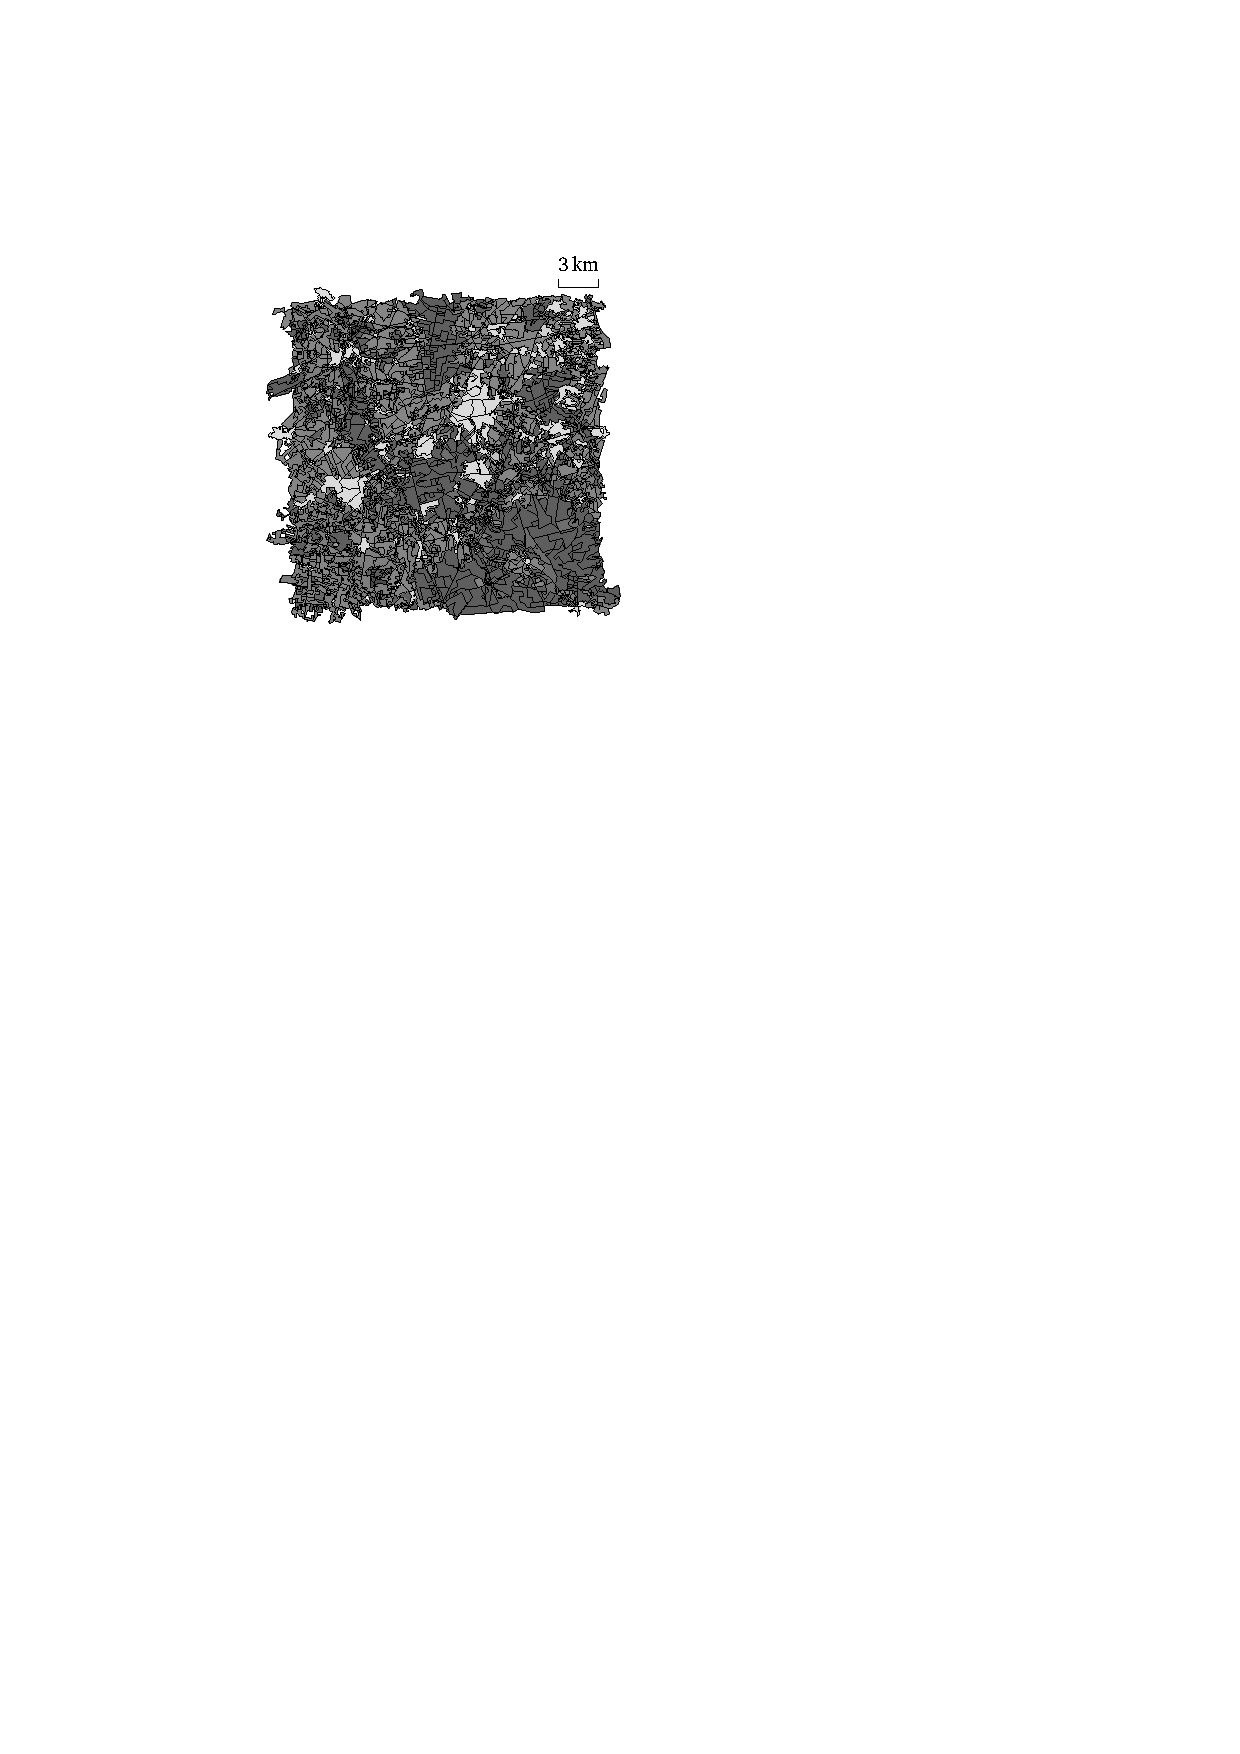
\includegraphics[page=1]{AreaAgg_Data}
\caption{Start map, $5{,}537$ polygons, \\
	at scale $1:50{,}000$}
\end{subfigure}
\hfill
\begin{subfigure}[b]{.49\textwidth}
\centering
\includegraphics[page=2]{AreaAgg_Data}
\caption{Goal map, $734$ polygons, \\
	at scale $1:250{,}000$}
\end{subfigure}
%
%It doesn't work to directly use 
%\vspace{\baselineskip} for subfigures.
\par\vspace{\baselineskip} %Leave a gap	figures
%
\begin{subfigure}{\textwidth}
\centering
\includegraphics[page=3]{AreaAgg_Data}
\caption{The 20 land-cover types appearing in our data}
\end{subfigure}
\caption{The data of our case study.}
\label{fig:AreaAgg_Data}
\end{figure}

\begin{figure}[tb]
\centering
\includegraphics[page=4]{AreaAgg_Data}
\caption{Distribution of the region sizes:
	the $y$-axis shows how many regions 
	of a given size range are contained in our dataset.}
\label{fig:AreaAgg_NumRegion}
\end{figure}

\begin{figure}[tb]
\centering
\includegraphics[page=5]{AreaAgg_Data}
\caption{The tree of type hierarchy used in our case study.
	For example, the distance between 
	types \emph{village} and \emph{farm land} is~$6$.}
\label{fig:AreaAgg_TypeDistances}
\end{figure}

\subsection{Using Costs of Type Change and Compactness}
\label{sec:AreaAgg_CaseStudy1}

As illustrated in \sect\ref{sec:AreaAgg_Combining},
we compare the \Astar algorithm and 
the greedy algorithm using $g_1(\Pnode)$,
which is a combination of the costs 
of type change and compactness (see \eq\ref{eq:g_1}).
For \Astar, we overestimated 
whenever we could not find a solution after 
having visited~$W$ nodes 
(see \sect\ref{sec:AreaAgg_AStar}).
We tried~$W=200{,}000$ and~$W=400{,}000$
(if we could use more main memory, 
then we could test by using some larger~$W$). 
The results are shown in 
Table~\ref{tab:AreaAgg_CaseStudy1_Statistics}.
%
Comparing to \Astar, 
the greedy algorithm visited 
fewer nodes and arcs in graph~$G_\mathrm{S}$ 
and used much less time.
However, \Astar managed to find solutions with 
lower total cost,~$117.3$ (or~$117.2$), 
which is~$2.8\%$ less than 
the total cost of the greedy algorithm,~$120.7$.
%
When~$W=200{,}000$, we are sure that 
we have found optimal solutions 
for~$702$ of the~$734$ regions ($95.6\%$),
while the greedy algorithm solved 
only~$408$ ($55.6\%$) to optimality;
see column \#OS in 
Table~\ref{tab:AreaAgg_CaseStudy1_Statistics}.
For the other~$32$ regions, 
both algorithms have found feasible solutions 
(see column \#FS in 
Table~\ref{tab:AreaAgg_CaseStudy1_Statistics}).
Although some of the feasible solutions may also be optimal,
we cannot verify that only from the cost values.


\begin{table*}[tb]
\caption{A comparison of the greedy algorithm and \Astar		
	when using cost function~$g_1$ (see \eq\ref{eq:g_1}).
	For \Astar, we used two settings, 
	i.e.,~$W=200{,}000$ and~$W=400{,}000$.
	%
	Column~\#OS shows the numbers of regions 
    that we obtained optimal solutions.   
	%
	Column~\#FS presents 
    the numbers and the percentages of regions (out of~$N=734$) 
    that we obtained feasible (non-optimal) solutions.
	%
	Variable~$k_\mathrm{sum}$ is 
	the total number of repetitions.
	%
	Columns~\#nodes and~\#arcs are the total 
	numbers of nodes and arcs that \Astar visited  
	(for instances where we needed overestimation, 
	only the final attempt was counted).
	%
	Columns~$\sum g_\mathrm{type}$, $\sum g_\mathrm{comp}$, 
	and~$\sum g_1$
	respectively denotes the sums of~$g_\mathrm{type}(\Pgoal)$,
	$g_\mathrm{comp}(\Pgoal)$, and~$g_1(\Pgoal)$ 
	over all the~$734$ instances 
	(see \eqs\ref{eq:g_type}, \ref{eq:g_comp}, 
	and~\ref{eq:g_1}).
	%
	The percentage in the \emph{Time}
	column is the fraction of the runtime 
    spent on solving the instances
	that we obtained feasible solutions.
    For \Astar, the time needed for overestimation
    is included.
}
\label{tab:AreaAgg_CaseStudy1_Statistics}
\centering
\fontsize{9}{11}\selectfont %for my thesis; should before \setlength{\tabcolsep}{0.7ex}
\setlength{\tabcolsep}{0.7ex}
\begin{tabular}{lRRRCCCCCd{3.7}}
\toprule
\multicolumn{1}{l}{Methods} &
\multicolumn{1}{c}{\#OS} &
\multicolumn{1}{c}{\#FS} &
\multicolumn{1}{r}{$k_\mathrm{sum}$} &  
\multicolumn{1}{c}{\#nodes} & 
\multicolumn{1}{c}{\#arcs} & 
\multicolumn{1}{c}{$\sum g_\mathrm{type}$} & 
\multicolumn{1}{c}{$\sum g_\mathrm{comp}$} & 
\multicolumn{1}{c}{$\sum g_1$} & 
\multicolumn{1}{c}{Time (min)} \\ 
\midrule
Greedy 	& 408 
&326~(44.4\%) 
&             &5.5\cdot 10^3   &4.8\cdot 10^3   
&53.2         &188.2           &120.7           &0'1~(74.6\%)\\
%
%
\AstarTwo	& 702 
&  32~(\parbox{\widthof{$4$}}{$\,$}$4.4\%$) 
& 102 &  3.6\cdot 10^6 &    5.7\cdot 10^6	
& 51.4 & 183.2 & 117.3 & 51'6~(93.2\%)\\
%
%
\AstarFour	& 704 
&  30~(\parbox{\widthof{$4$}}{$\,$}$4.1\%$)
&  89 &  6.5\cdot 10^6 &    9.8\cdot 10^6
& 51.4 & 183.1 & 117.2 & 93'1~(95.5\%)
\\ \bottomrule			
\end{tabular}
\end{table*}


In accordance with \sect\ref{sec:AreaAgg_AStar}, 
for region with ID~$i$ 
we define~$k_i$ as the least number of repetitions 
that we do to find a feasible solution. 
We define the total number of repetitions 
as~$k_\mathrm{sum}=\sum_{i=1}^N k_i$, 
where~$N=734$ is the number of the regions.
After increasing~$W$ to~$400{,}000$, 
\Astar found optimal aggregation sequences 
for only two more regions, 
but $k_\mathrm{sum}$ decreased quite a bit, 
from~$102$ to~$89$. 
The numbers of regions that needed certain
overestimation steps are shown in 
\fig\ref{fig:AreaAgg_OverStats}. 
Besides, \Astar visited more arcs and nodes, 
used more time, 
but got (slightly) less cost when increasing~$W$ to~$400{,}000$.
Although the number of regions 
that needed overestimation is relatively small, 
\Astar spent most of the running time 
on those few regions:~$4.4\%$ and~$4.1\%$ of the regions 
caused~$93.2\%$ and~$95.5\%$ of the total running time, 
respectively 
(see Table~\ref{tab:AreaAgg_CaseStudy1_Statistics}).

\begin{figure}[tb]
\centering

\includegraphics[page=2]{AreaAgg_CaseStudy1_Plot}
\caption{The numbers of regions where \Astar was 
	forced to use the given overestimation parameters
	in order to find a solution 
	without exploring more than 
	$W \in \{200{,}000;~400{,}000\}$ 
	nodes of the subdivision graph.}
\label{fig:AreaAgg_OverStats}
\end{figure}

The details of some regions are presented in 
Table~\ref{tab:CostsInDetail}.
According to the entries with overestimation factor $K_i=0$, 
we often have 
ratios~$R_\mathrm{type}=1$ and~$R_\mathrm{comp}>1$.
When factor~$K_i=0$, we did not overestimate for region~$i$.
The estimated cost must be smaller or equal to the exact cost,
which results in~$R_\mathrm{type}\ge 1$ 
and~$R_\mathrm{comp}\ge 1$.
Ratio~$R_\mathrm{type} = 1$ means that our estimation for the 
cost of type change is the best.
A larger~$R_\mathrm{comp}$ means 
a poorer estimation for the cost of shape.

\begin{table*}[tb]
\caption{The costs in detail of some regions, 
	where~$W=200{,}000$.  
	Parameters~$n$ and~$m$ are the numbers of patches and 
	adjacencies on the start map, respectively.
	Parameter $K$ is the overestimation factor, 
	defined in \sect\ref{sec:AreaAgg_Preliminaries}. 
	We evaluate the quality 
	of our estimations for type change and 
	compactness by listing the numbers~
	$R_\mathrm{type}=g_\mathrm{type}(\Pgoal)
	/h_\mathrm{type}(\Pstart)$ and~
	$R_\mathrm{comp}=g_\mathrm{comp}(\Pgoal)
	/h_\mathrm{comp}(\Pstart)$. 
	Note that if~$h_\mathrm{type}(\Pstart)=0$,
    then we have~$g_\mathrm{type}(\Pgoal)=0$; 
	in this case, we define~$R_\mathrm{type}=1$.
	The marked entries are discussed in the text.
}
\label{tab:CostsInDetail}
\centering

\includegraphics[page=3]{AreaAgg_CaseStudy1_Plot}
\end{table*}


According to columns~$n$ and~$K$ of \tab\ref{tab:CostsInDetail},
\AstarTwo managed to find optimal solutions 
for all the regions with fewer than~$15$ polygons,
and only found feasible solutions 
for any region with more than~$21$ polygons.
Among the~$702$ regions that 
\AstarTwo solved to optimality,
the greedy algorithm failed to 
find optimal solutions for~$294$ regions.
Solutions of the greedy algorithm cost
at most~$41.7\%$ more than 
solutions of \AstarTwo;
for region~$85$, the greedy algorithm yields 
a solution of cost~$0.777$, 
while the solution of \AstarTwo has cost~$0.548$
(see \fig\ref{fig:AreaAgg_CaseStudy1_Rg85}).
As the patches in the two sequences are the same,
the two results have the same cost of compactness.
The main difference is the choice of the first step, 
from~$8$ patches to~$7$.
When aggregating the smallest patch on the start map
with the surrounding patch,
our greedy algorithm chooses the type 
which is closer to the goal type.
In this case, the smallest patch has type~$5112$, and the 
surrounding one has~$2112$.
The type of the goal patch is~$4102$.
According to \fig\ref{fig:AreaAgg_TypeDistances},
type distances~$d_\mathrm{type}(5112,4102)=4$ and~$d_\mathrm{type}(2112,4102)=6$.
As a result, our greedy algorithm uses~$5112$ 
as the type for the new patch. 
This choice is a big mistake 
because the type of the largest patch on the start map
will have to be changed twice during the aggregation.
These changes cause a cost more than the sequence obtained by 
\AstarTwo, 
where the largest patch on the start map is changed to 
the target type directly.

Among the $32$~regions that 
\AstarTwo failed to solve optimally,
the greedy algorithm outperformed \AstarTwo 
for~$15$ regions ($46.9\%$).
%
Among these, solutions of the greedy algorithm 
cost at most~$15.9\%$ less than solutions of \AstarTwo;
for region~$543$, the greedy algorithm yields 
a solution of cost~$0.112$, 
while the solution of \AstarTwo costs~$0.134$. 
For this instance, 
\AstarTwo used overestimation parameter~$K=7$
(marked in \tab\ref{tab:CostsInDetail}).
\fig\ref{fig:AreaAgg_CaseStudy1_Rg543} shows 
some intermediate results obtained by
\AstarTwo and the greedy algorithm.
Interestingly, the two methods produced the same sequence until 
there were~$8$ patches left.
Then due to the overestimation, 
\AstarTwo did some bad moves
because the bad aggregation sequence still seemed better 
than other sequences.
In contrast, the greedy algorithm was looking for locally good 
aggregations.
%
Among the~$32$ regions that 
\AstarTwo failed to solve optimally,  
solutions of the greedy algorithm cost at most~$17.4\%$ 
more than solutions of \AstarTwo; 
for region~$155$, the greedy algorithm yields 
a solution of cost~$0.372$, while
the solution of \AstarTwo costs~$0.317$
(marked in \tab\ref{tab:CostsInDetail}).

Finally, an optimal aggregation sequence of region~$53$
(third-last row in \tab\ref{tab:CostsInDetail})
obtained by \AstarTwo
is shown in \fig\ref{fig:AreaAgg_CaseStudy1_Rg53}.

\begin{figure}[tb]
\centering
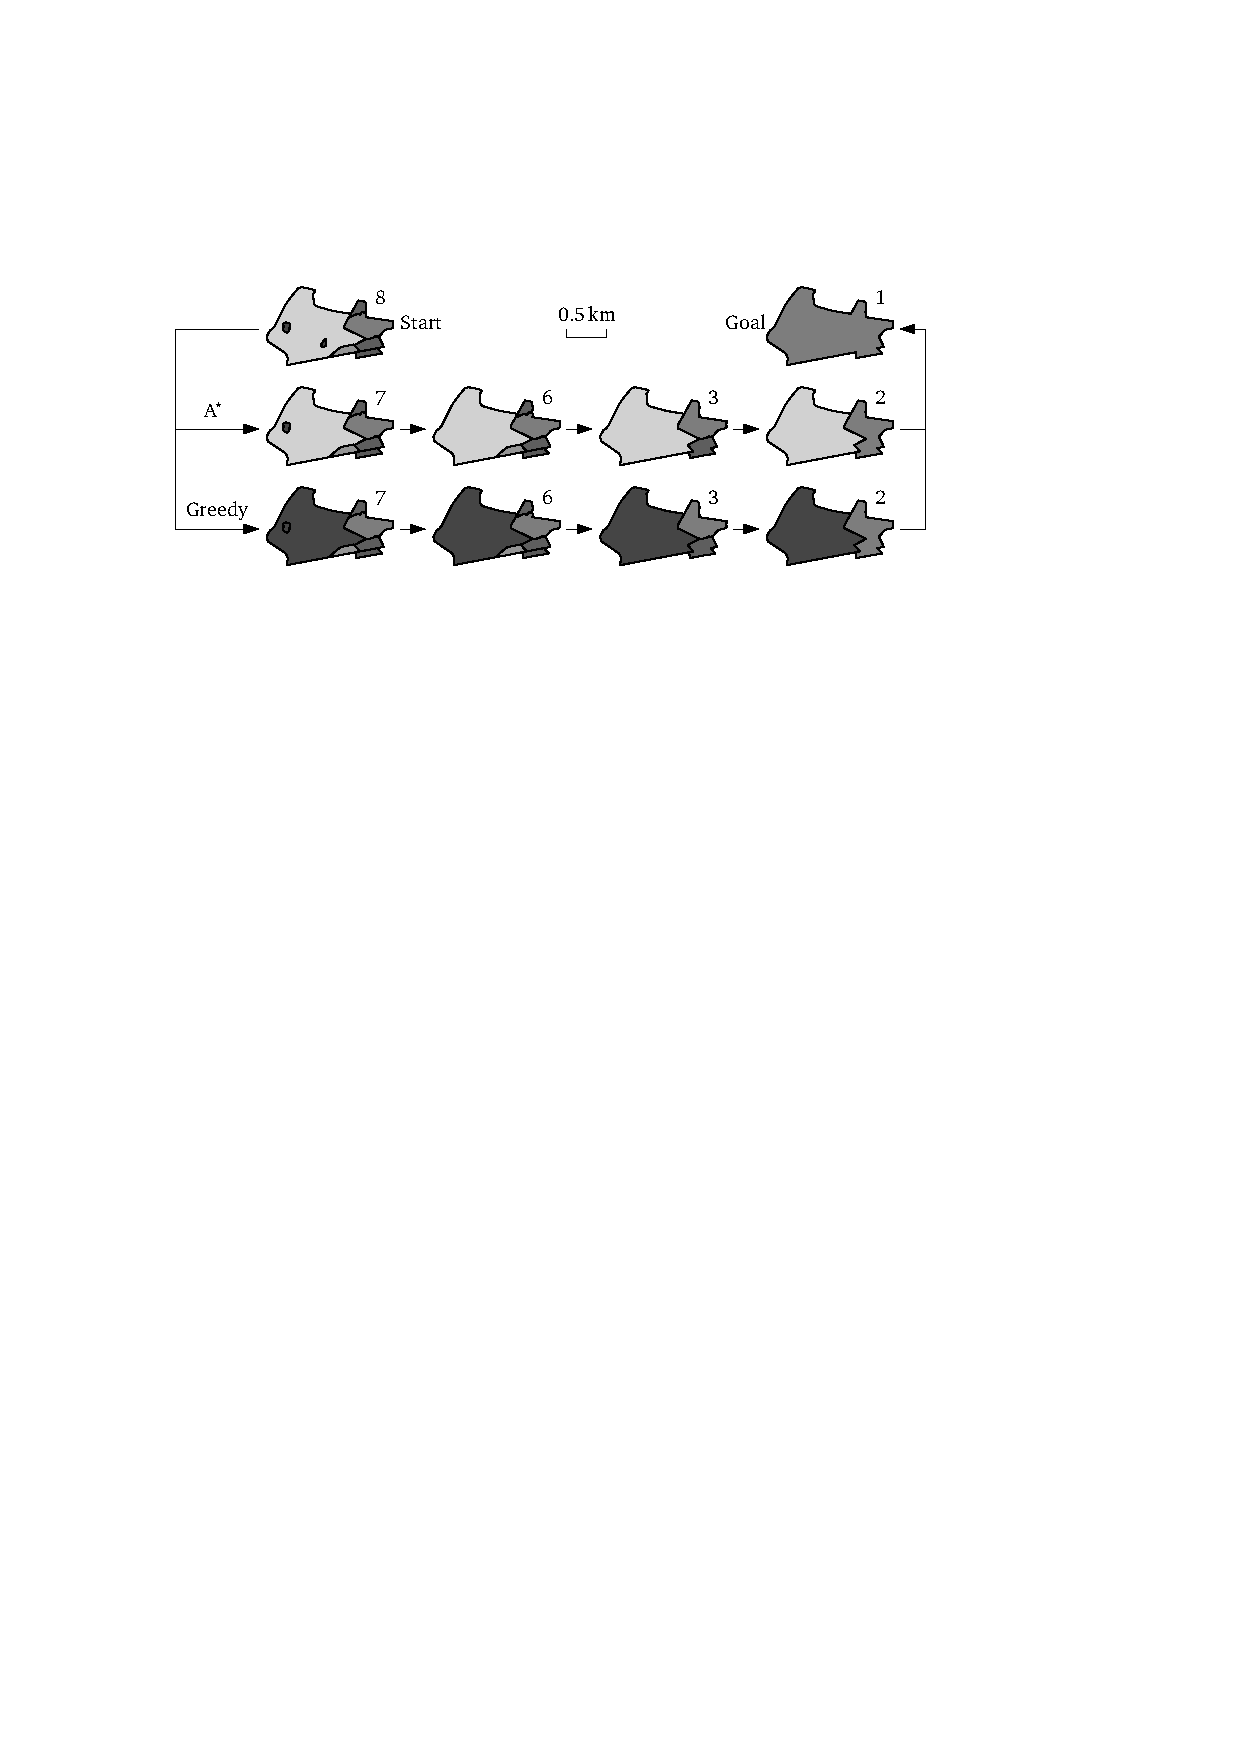
\includegraphics[page=1]{AreaAgg_CaseStudy1}
\caption{Aggregation sequences of region~$85$ 
	obtained by \Astar and the greedy algorithm.
	In order to save space, we did not show the results 
	when there are~$4$ or~$5$ patches, 
	which one can easily deduce.
	The numbers indicate the numbers of patches.
    %
    In the sequence obtained by \Astar, 
    the type of the largest polygon on the start map 
    changed only once, which is good; 
    while the type of the largest polygon changed twice 
    in the sequence obtained by the greedy algorithm.}
\label{fig:AreaAgg_CaseStudy1_Rg85}
\end{figure}

\begin{figure}[tb]
\centering
\includegraphics[page=2]{AreaAgg_CaseStudy1}
\caption{Some intermediate subdivisions of region~$543$ 
	obtained by \Astar and the greedy algorithm.
	In the sequence obtained by \Astar, 
	a pair of circles or a pair of squares indicates that
	the two parts are actually in the same patch.
	The numbers indicate the numbers of patches.
}
\label{fig:AreaAgg_CaseStudy1_Rg543}
\end{figure}


\begin{figure}[tb]
\centering
\includegraphics[page=3]{AreaAgg_CaseStudy1}
\caption{An optimal sequence of intermediate subdivisions 
	of region~$53$ obtained by \Astar 
	using the costs of type change and compactness.		 
	The numbers indicate the numbers of patches.		
}
\label{fig:AreaAgg_CaseStudy1_Rg53}
\end{figure}


%\todo[inline]{It turned out that the objective function $g$ 
%seems rather robust
%	against changes of~$\lambda$.  For region~77, we 
%	varied~$\lambda$ in
%	the range $\{0.1,0.5,0.9\}$, but the resulting aggregation 
%	sequences
%	stayed almost the same.  When we used even larger 
%	values 
%	for~$\lambda$ (e.g.,~$0.99$), the (good) influence of type 
%	change was mitigated 
%	and, as a
%	result, we needed to overestimate (with factor~$K=8$).}




\subsection{Using Costs of Type Change and Length}
\label{sec:AreaAgg_CaseStudy2}

We compare the greedy algorithm, \Astar, and ILP
using~$g_2(\Pnode)$,
a combination of the costs 
of type change and length (see \eq\ref{eq:g_2}).
For \Astar, we overestimated 
whenever we could not find a solution after 
having visited~$W=200{,}000$ nodes 
(see \sect\ref{sec:AreaAgg_AStar}).
The most time-consuming instance for \Astar was region~$94$,
for which \Astar took~$104.1\,$s (including repetitions)
to find a feasible solution 
with overestimation factor~$K=31$.
To avoid waiting too long,
we set the time limit to~$100\,$s 
for our ILP to run on one region.
Note that the time limit included
the time that our ILP used 
to set up the variables and constraints
(see \sects\ref{sub:AreaAgg_variables} 
and~\ref{sub:AreaAgg_Constraints}).
If no optimal solution was found in this time limit,
a feasible solution (if found) would be returned.
For some large instances, 
the ILP could not find any solution.

Using a similar format as in 
\tab\ref{tab:AreaAgg_CaseStudy1_Statistics},
we present the statistics in 
\tab\ref{tab:AreaAgg_CaseStudy2_Statistics}.
\Astar found optimal solutions 
for~$695$ of the~$734$ regions ($94.7\%$).
Again, it spent most of the running time 
on the few regions that needed 
overestimation:~$5.3\%$ of the regions 
caused~$92.3\%$ of the total running time.
The solutions by \Astar cost~$438.2$ in total, 
which is~$3.9\%$ less than~$455.8$, 
the total cost of the solutions by the greedy algorithm.

\begin{table*}[tb]
\caption{A comparison of the greedy algorithm, 
    the \Astar algorithm, and the ILP-based algorithm		
	when using cost function~$g_2$ (see \eq\ref{eq:g_2}).
	The notations are the same as in
	\tab\ref{tab:AreaAgg_CaseStudy1_Statistics}.
	%
	Columns~$\sum g_\mathrm{type}$, $\sum g_\mathrm{lgth}$, 
	and~$\sum g_2$
	respectively represent the sums of~$g_\mathrm{type}(\Pgoal)$,
	$g_\mathrm{lgth}(\Pgoal)$, and~$g_2(\Pgoal)$ 
	over all the~$734$ instances 
	(see \eqs\ref{eq:g_type}, \ref{eq:g_length}, 
	and~\ref{eq:g_2}).
}
\label{tab:AreaAgg_CaseStudy2_Statistics}
%	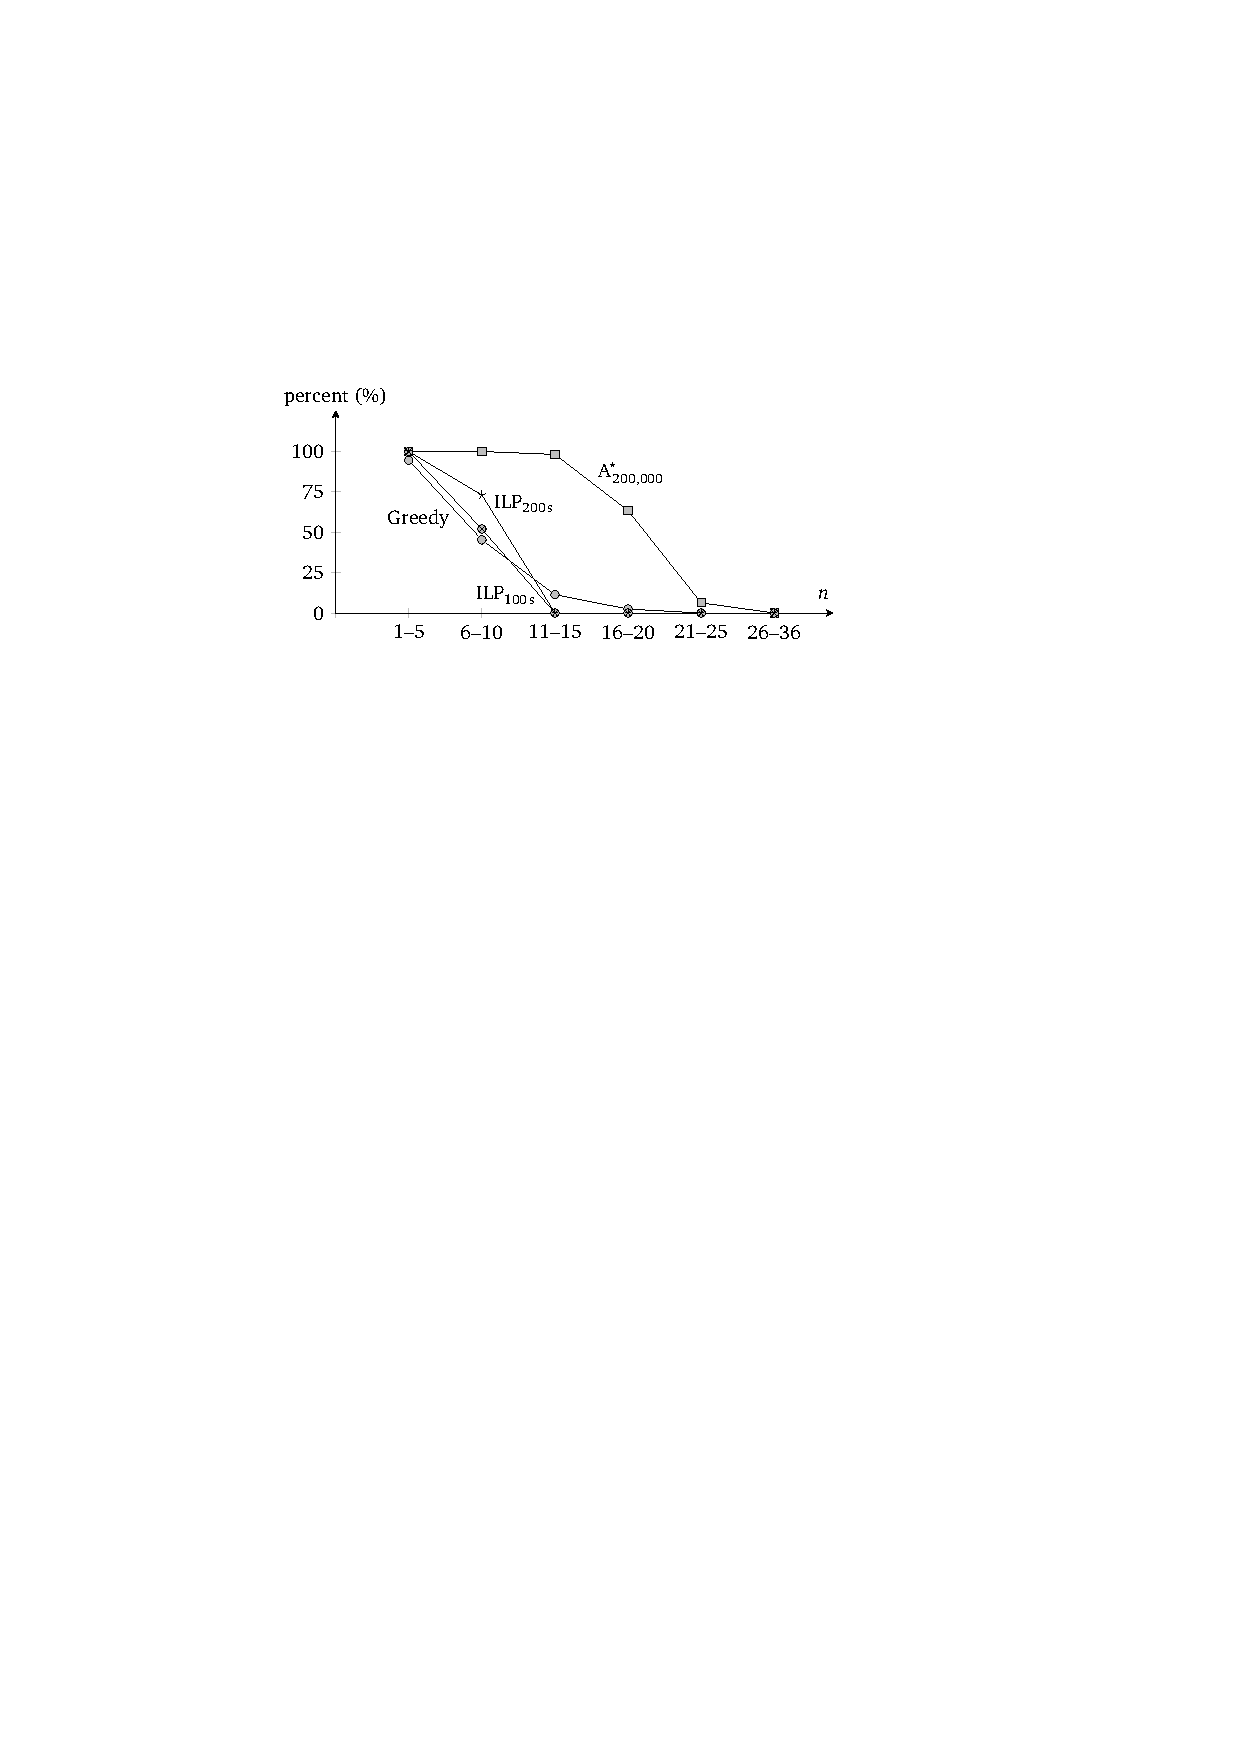
\includegraphics[page=1]{AreaAgg_CaseStudy2_Plot}
\centering
\fontsize{9}{11}\selectfont %for my thesis; should before \setlength{\tabcolsep}{0.7ex}
\setlength{\tabcolsep}{0.7ex}
\begin{tabular}{lRRRCCCCCd{3.7}}
\toprule
\multicolumn{1}{l}{Methods} &
\multicolumn{1}{c}{\#OS} &
\multicolumn{1}{c}{\#FS} &
\multicolumn{1}{r}{$k_\mathrm{sum}$} &  
\multicolumn{1}{c}{\#nodes} & 
\multicolumn{1}{c}{\#arcs} & 
\multicolumn{1}{c}{$\sum g_\mathrm{type}$} & 
\multicolumn{1}{c}{$\sum g_\mathrm{lgth}$} & 
\multicolumn{1}{c}{$\sum g_2$} & 
\multicolumn{1}{c}{Time (min)} \\ 
\midrule
Greedy 		 &430             
&304~(41.4\%)    
&            &5.5\cdot 10^3   &4.8\cdot 10^3   
&53.0        &858.5           &455.8           &0'1~(70.7\%)\\
%
%
\AstarTwo	& 695
& 39~(\parbox{\widthof{$4$}}{$\,$}$5.3\%$)	
& 150 	& 3.7\cdot 10^6 & 7.3\cdot 10^6 
& 52.0 	& 824.5 & 438.2 &44'8~(92.3\%)	\\
%
%
\ILPOne		& 449
& 69~(\parbox{\widthof{$4$}}{$\,$}$9.4\%$)  			 	
&		&				&				
&		&		&		& 421'5~(27.3\%) \\
%
%
\ILPTwo		& 475
& 57~(\parbox{\widthof{$4$}}{$\,$}$7.8\%$)  			 	
&		&				&				
&		&		&		& 719'2~(26.4\%) \\ 
\bottomrule
\end{tabular}
\end{table*}




\Astar managed to find optimal solutions 
for all the regions with fewer than~$15$ polygons, and 
found only feasible solutions for the regions 
with more than~$21$ polygons.
%
In the~$39$ (out of~$734$) regions 
that \Astar failed to solve optimally,
the greedy algorithm outperformed \Astar 
for~$8$ regions~($20.5\%$), 
which is~$26.4\%$ less comparing to the first experiment ($46.9\%$).
%
\ILPOne managed to find optimal solutions 
for all the regions with fewer than~$8$ polygons,
and failed to find optimal solutions
for any region with more than~$8$ polygons.
In none of the~$39$ regions 
that \Astar failed to solve optimally
did \ILPOne find a feasible solution.
Overall, \ILPOne 
found optimal solutions for~$449$ regions
and found feasible solutions for~$69$ regions.
The distributions of these regions are shown in
\figs\ref{fig:AreaAgg_CaseStudy2_Percentage_Optimal}
and~\fig\ref{fig:AreaAgg_CaseStudy2_Percentage_Feasible}
There are~$216$ regions for which 
our \ILPOne failed to find any solution.
For~$22$ of those regions, 
we did not have enough main memory 
to set up the variables and constraints;
each of these regions has~$21$ polygons at least.
For~$67$ of those regions, 
our \ILPOne ran out of the main memory 
before finding any feasible solution;
these regions have~$14$ to~$20$ polygons.
Note that we allowed our program to use~$3\,$GB 
of the main memory at most.
For~$123$ of the $216$~regions, 
\ILPOne failed to find any solution
during the time limit;
these regions have~$9$ to~$13$ polygons.
For the remaining~$4$ regions, 
the reason of our ILP's fail is unclear 
due to the fact that 
the solver CPLEX is like a black box for us.
After we increased the time limit to~$200\,$s for each region, 
\ILPTwo solved~$475$ regions to optimality, which 
is~$26$ regions more than using \ILPOne.
Every of the~$26$ regions has~$6$ to~$10$ polygons.
\fig\ref{fig:AreaAgg_CaseStudy2_Percentage_Optimal}
shows the percentages of the regions 
that are solved optimally by the three algorithms.
\fig\ref{fig:AreaAgg_CaseStudy2_Percentage_Feasible} 
shows the percentages of the regions 
that the three algorithms found feasible solutions.
\fig\ref{fig:AreaAgg_CaseStudy2_ILP} shows 
the number of regions for which 
the ILP found optimal, feasible, or no solutions 
when using the two time limits, i.e., $100\,$s and~$200\,$s.


\begin{figure}[tb]
\centering
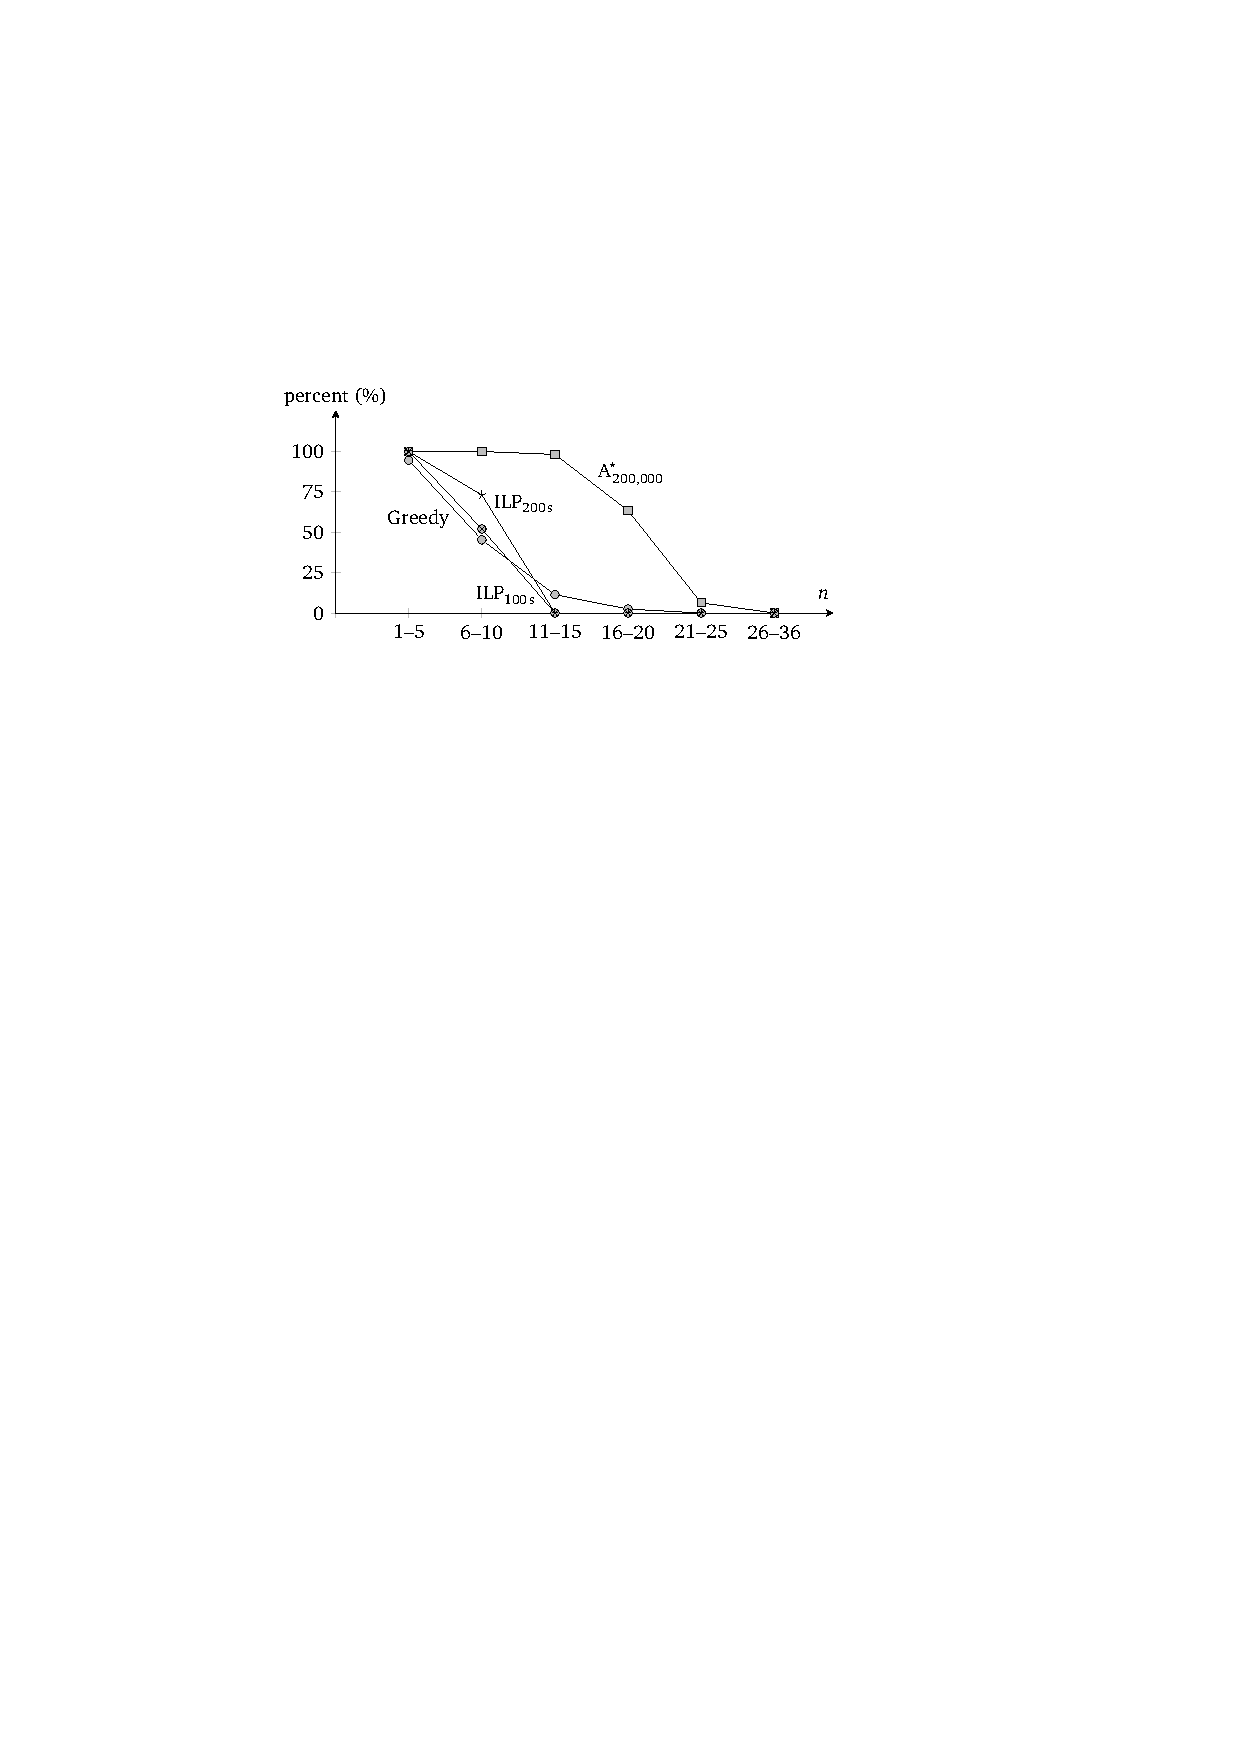
\includegraphics[page=1]{AreaAgg_CaseStudy2_Plot}
\caption{The percentage of regions that were solved 
	optimally by the greedy algorithm, \Astar, and our ILP.
	Note that the numbers of regions according to~$n$ 
	(the number of polygons on the start map in one region) 
	are shown in \fig\ref{fig:AreaAgg_NumRegion}.}
\label{fig:AreaAgg_CaseStudy2_Percentage_Optimal}
%
\par\vspace{\baselineskip} %Leave a gap	between figures
%
\centering
\includegraphics[page=2]{AreaAgg_CaseStudy2_Plot}
\caption{The percentage of regions for which we found at 
	least feasible solutions by the three algorithms.
	Note that the numbers of regions according to~$n$ 
	(the number of polygons on the start map in one region) 
	are shown in \fig\ref{fig:AreaAgg_NumRegion}.}
\label{fig:AreaAgg_CaseStudy2_Percentage_Feasible}
\end{figure}

\begin{figure}[tb]
\centering
\includegraphics[page=3]{AreaAgg_CaseStudy2_Plot}
\caption{The number of regions for which
	our ILP found optimal, feasible, or no solutions 
	when using time limits~$100\,$s and~$200\,$s.
	Using more time, our ILP was able to 
	solve more instances to optimality.}
\label{fig:AreaAgg_CaseStudy2_ILP}
\end{figure}

Among all the instances that were solved to optimality by \Astar
in both experiments (i.e., \sects\ref{sec:AreaAgg_CaseStudy1} 
and~\ref{sec:AreaAgg_CaseStudy2}),
region~$358$ (marked in \tab\ref{tab:CostsInDetail})
is the largest one.
In both experiments, the cost of type change is~$0.044$.
The optimal aggregation sequences for this region
obtained by using costs~$g_1$ and~$g_2$
are shown in \fig\ref{fig:AreaAgg_CaseStudy2_Rg358}.
We, however, noticed some unpleasant aggregates.
The step from~$8$ patches to~$7$ patches 
when using cost function~$g_1$ is a bad move
(see \fig\ref{fig:AreaAgg_CaseStudy2_Rg358}b).
Instead we expect the result of 
\fig\ref{fig:AreaAgg_CaseStudy2_Rg358}a.
Using cost function~$g_2$, we had a similar problem. 
The subdivision with~$7$ patches is such an example,
where we expect the result of 
\fig\ref{fig:AreaAgg_CaseStudy2_Rg358}c.
In an earlier version of this chapter \parencite[see][]{Peng2017AStar},
we tried a combination of minimizing type changes 
and maximizing the sum of the smallest compactness values, 
over the whole sequence.
For that objective, we had a similar problem as 
in \fig\ref{fig:AreaAgg_CaseStudy2_Rg358}b.
This problem, however, can be fixed easily 
by forbidding two patches to aggregate 
if their common boundary is too short.
Moreover, there are two more possible solutions.
First, we could integrate the shared length
into our cost function, as did by \textcite{vanOosterom2005}.
Second, we could weight the cost of shape more heavily
(i.e., increasing weight factor~$\lambda$ of 
\eqs\ref{eq:g_1} and~\ref{eq:g_2}).
According to our experiences, 
the weight factor that we applied defines a reasonable trade-off 
between the different conflicting objectives, 
when considering a solution as a whole. 
However, we are far from claiming that 
the applied weight factor has been optimally chosen. 
This would probably require a user study.

\begin{figure}[h!tb]
\centering
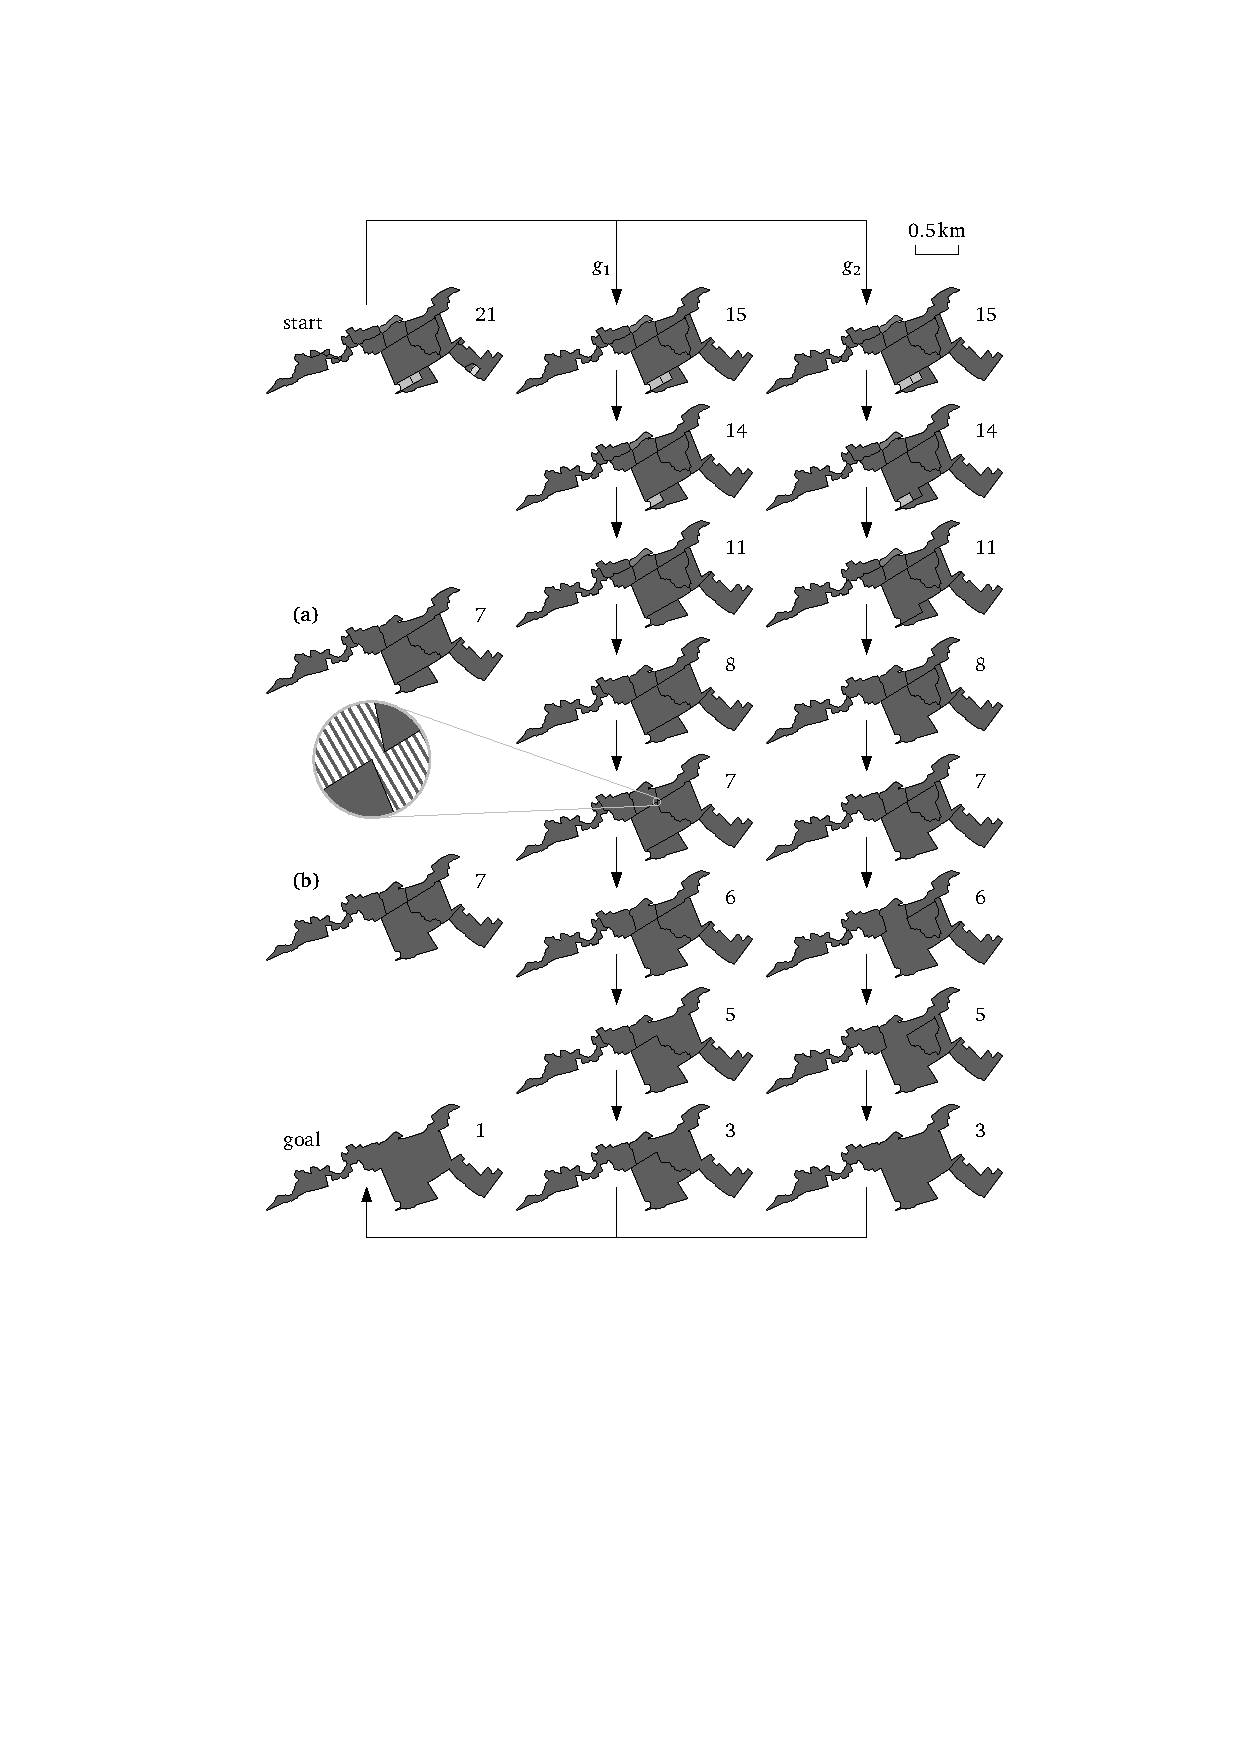
\includegraphics[page=1]{AreaAgg_CaseStudy2}
\caption{Some intermediate subdivisions of region~$358$ 
	obtained by \Astar with different cost functions.
	The numbers indicate the numbers of patches.
    The step from $8$ patches to $7$ patches 
    when using cost function~$g_1$ is a bad move; see figure (b). 
    Instead, we expect the result of figure (a). 
    Using cost function~$g_2$, we had a similar problem. 
    The subdivision with $7$ patches is such an example, 
    where we expect the result of figure (c).
}
\label{fig:AreaAgg_CaseStudy2_Rg358}
\end{figure}


%\todo{chart: memory use of greedy, A*, and ILP}

\section{Concluding Remarks}
\label{sec:AreaAgg_Conclusions}
In this chapter, we investigated the problem of 
finding optimal sequences for area aggregation.
We compared three methods to solve this problem, namely, 
a greedy algorithm, \Astar, and an ILP-based algorithm.
The greedy algorithm is used as a benchmark.
Unsurprisingly, it ran faster than the other two methods by far.
According to our experiments, \Astar found area aggregation 
sequences
with the least total cost over all regions.
For some instances, however, \Astar had to overestimate
in order to find feasible solutions.
Compared to the greedy algorithm, 
\Astar reduced the total costs by~$2.8\%$ and~$3.9\%$
in the two experiments.
Although the amount is small, it is worth to use \Astar
because optimization methods can help us 
to evaluate the quality of a model 
\parencite{Haunert2017Label,Haunert2008Assuring,Haunert2016Optimization}.
For example, \fig\ref{fig:AreaAgg_CaseStudy2_Rg358}b shows that
even an \emph{optimal} sequence can be bad.
If it were not for \Astar, 
we could not tell if the bad result was caused 
by the greedy algorithm or the model.
Because of \Astar, we are sure that the bad result is from
our model of minimizing the 
type change and the compactness.
The ILP-based algorithm finds optimal solutions for some regions,
but for some of the other regions 
it cannot even find a feasible solution.
Compared to the ILP-based algorithm,
\Astar used less memory 
yet found optimal solutions for more regions.

%\todo[inline]{estimate compactness based on length; cauchy 
%schwarz}

Our \Astar has a good estimation for the cost of type 
change, which helps a lot to reduce the search space. 
Our estimation for the cost of shape 
(compactness or length) is poor.
There are two ways to improve \Astar
in terms of solving more instances to optimality 
while using the same limit of main memory.
First, during the searching we can forget a node of the graph
(see \fig\ref{fig:AreaAgg_SubdivisionName})
if all the neighbors of this node have been visited.
By testing a case, we learned that half of the nodes can be 
forgotten during the pathfinding process.
In this way, we can release some main memory 
and visit more nodes.
Once we arrive at the goal, 
we know the cost for 
an optimal solution (the least cost).
As many visited nodes have been forgotten, 
we do not have the shortest path so far.
We need to run \Astar again.
This time we know for sure that 
a path is not optimal if its cost, 
the sum of the exact cost and the estimated cost, 
is more than the least cost 
(of the optimal solution found previously).
Consequently, we are able to prune some branches earlier 
than the first time we run \Astar.
In this way, we manage to save some main memory.
As a result, we are more likely to find optimal solutions
when the main memory is limited.
Second, if we obtain a solution based on overestimation, 
then we know the cost of this non-optimal solution.
We may decrease the overestimation factor by pruning the branches
that cost more than the non-optimal solution.


We may speed up our ILP-based algorithm using a so-called 
cutting-plane approach as \textcite{Oehrlein2017Aggregation}.
Also, we can add more constraints to
reduce the choices of variables.
For example, assignment to a given center~$r$ is symmetric, 
hence we have
\begin{equation*}
\label{eq:CstrZX}
z_{t,p,q,r}= z_{t,q,p,r} \qquad
\forall t \in {T} \setminus \{1,n\}, 
\forall p, q, r \in P.
\end{equation*}
Whether adding such kinds of constraints always
speeds up our ILP is not clear
because the solver, CPLEX, is a black box to us.
Although integer linear programming may be not good at 
finding optimal sequences for area aggregation,
it is relatively easy to formulate problems as ILPs.
As stated by \citet[p.~861]{Cormen2009}, 
``an efficient algorithm designed specifically for a problem 
will often be more efficient than 
linear programming both in theory and in practice. 
The real power of linear programming comes from 
the ability to solve new problems.''

We may improve both the \Astar algorithm and the ILP-based 
algorithm by integrating the greedy algorithm.
The idea is that we use the greedy algorithm to find 
a solution. 
Then we can use the cost of the solution as an upper bound to 
prune the branches of \Astar and the ILP. 
Once we see that
the cost of a branch is larger than the upper bound,
we can ignore that branch  
because it will not yield an optimal solution.



In cartography, there are many more requirements 
for area aggregation.
For example, one requirement is 
to keep important land-cover areas for a longer time
(such as a settlement surrounded by farmlands).
This requirement can be achieved by incorporating the idea of
\textcite{Dilo2009tGAP}.
They gave each type a weight, 
then defined the importance of a patch 
by the product of the area size and the type weight.
While in our method, we used only the area size as importance.
%
Another requirement is that 
aggregating two areas may result in 
an area with a generalized type,
as did by \textcite{vanSmaalen2003}. 
For example, aggregating 
\emph{farmland} with \emph{hedge} 
yields an area with type \emph{vegetation}.
%
In our setting, we ignored the fact that
some features may inherently take linear forms
(e.g., rivers).
%
These issues can be considered in our future work.
%







%\chapter[<ToC-title>]{<Title>} 
\chapter[\AdminBoundToCTitle]{\AdminBoundTitle} 


\label{chap:Admin}

%appear at the top of the pages
\chaptermark{\AdminBoundChapterMark}

Nowadays people often browse through digital maps 
on computers or small displays to get geographic information. 
To understand maps better, 
users interactively zoom in and out to read maps 
from different levels. 
A typical strategy to support zooming is based on a
multiple representation database (MRDB).  
Such a database stores a discrete set of levels of detail (LODs) 
from which a user can query the LOD for a particular 
scale~\parencite{Hampe2004multiple}. 
A small set of LODs, however, leads to 
complex and sudden changes during zooming. 
%
Since these changes distract users, 
hierarchical schemes have been proposed
that generalize a more-detailed representation to obtain a
less-detailed one based on small incremental changes, 
e.g., the binary line generalisation tree (BLG-tree)
\parencite{vanOosterom2005} 
for line simplification or
the generalized area partitioning tree (GAP-tree)
\parencite{vanOosterom1995GAPTree}
for area aggregation.  
Such incremental generalization processes are represented 
in data structures 
that allow users to retrieve a map at any scale.  
Still, the generalization process consists of discrete steps 
and includes abrupt changes.  
Discrete steps can easily cause users to lose their
``mental map'' during interaction, which is annoying. 
To support continuous zooming, 
\textcite{vanKreveld2001} proposed five ways of gradual changes, 
which are \emph{moving}, \emph{rotating}, \emph{morphing}, 
\emph{fading}, and \emph{appearing}. 
These operations can be used 
in \emph{continuous generalization},
which generalizes a map to obtain a sequence of maps 
without abrupt changes.
To achieve continuous generalization, 
\textcite{Sester2004} suggested simplifying building
footprints based on small incremental steps and 
to animate each step smoothly;
\textcite{Danciger2009} investigated the growing of regions, 
meanwhile preserving their topology, area ratios, and
relative positions. 
The strategy of using two maps at different scales
to generate intermediate-scale maps has been studied in multiple
representations, e.g., with respect to the selection of roads or
rivers~\parencite{Girres2014}. 
Actually, this strategy is a key idea of the
morphing-based methods for continuous generalization. 
For instances, several authors have developed  
morphing methods for polylines~\parencite{Cecconi2003, 
Noellenburg2008, Peng2013LSA, Schneider2015,
Peng2012River,Deng2015}
and for raster 
maps~\parencite{Reilly2004,
	Pantazis2009b}.  % Add later: survey? \cite{Pantazis2009a}


\begin{figure}[tb]	
\centering
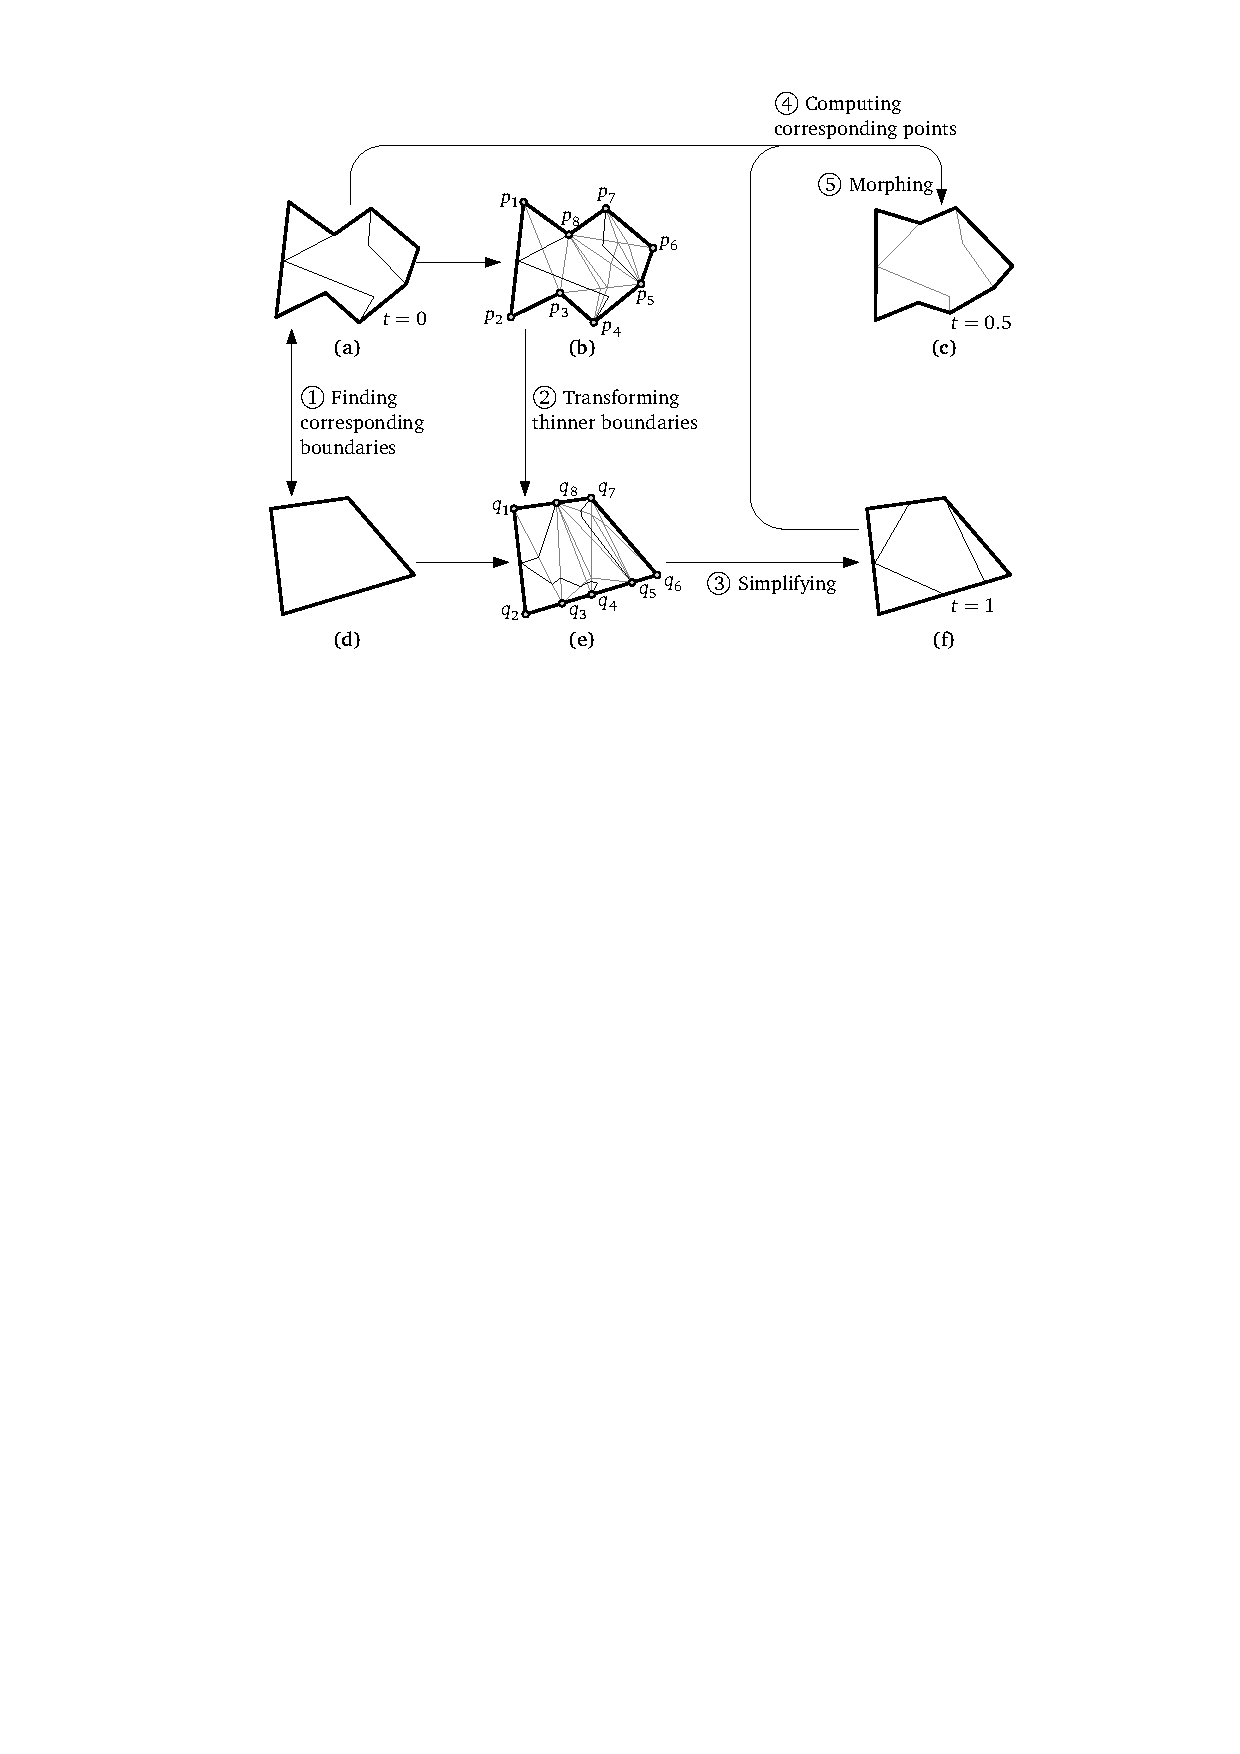
\includegraphics[page=1]{Admin_Introduction}
\caption{The framework of our method.
	The circled numbers indicate the steps. 
	(a)~The larger-scale administrative boundaries of a 
	region. 
	(d)~The smaller-scale administrative boundaries of the 
	same region as in~(a). 
	(b)~\&~(e) Constructing compatible triangulations for
	thicker polygons in~(a) and~(d) in order to 
	transform thinner boundaries in~(a) to~(e).
	(f)~The thinner boundaries are simplified from the 
	ones in~(e). 
	(c)~The result of continuous generalization
	by morphing when~$t=0.5$.
	The thinner boundaries in~(c) are being faded out.
	}
\label{fig:Admin_Introduction}
\end{figure}

Topological consistency is a property 
that must be attained in continuous generalization. 
In this chapter, we continuously generalize 
a two-level hierarchical subdivision---from 
a larger-scale map of administrative boundaries 
to a smaller-scale one.  
Our aim is to generate maps at any intermediate scales
without introducing topological conflicts.
For example, we try to generalize from
\fig\ref{fig:Admin_Introduction}a to
\fig\ref{fig:Admin_Introduction}d.
Our method consists of the following five steps.  


In step~\circled{1}, we find corresponding boundaries
between the two maps,
which are the thicker polylines in
\figs\ref{fig:Admin_Introduction}a 
and~\ref{fig:Admin_Introduction}d.  
We call the remaining boundaries, on the larger-scale map, 
\emph{unmatched} boundaries (see the
thinner polylines in \fig\ref{fig:Admin_Introduction}a). 
In order to achieve continuous generalization, 
we \emph{morph} (that is, deform continuously) 
between the thicker corresponding boundaries;
see for example \textcite{Noellenburg2008}.
The unmatched boundaries must be morphed in a way 
that is consistent with the thicker corresponding boundaries.  
As there is no correspondence for the unmatched ones, 
we generate the corresponding boundaries 
in steps~\circled{2} and~\circled{3}.

In step~\circled{2}, we transform the thinner boundaries 
based on \emph{compatible triangulations} (CTs); 
see \figs\ref{fig:Admin_Introduction}b 
and~\ref{fig:Admin_Introduction}e. 
Two triangulations are \emph{compatible} 
if they have a correspondence of their vertex sets as well as 
the two triangulations are topologically 
equivalent~\parencite{Surazhsky2001}. 
With CTs, 
we can transform a thinner boundary in one triangulation 
(see \fig\ref{fig:Admin_Introduction}b) 
to a boundary in the other triangulation 
by traversing the triangles correspondingly 
(see \fig\ref{fig:Admin_Introduction}e). 
Therefore, if there is no conflict in one triangulation, 
then there is no conflict in the other triangulation.
 

In step~\circled{3}, we simplify the thinner boundaries using
the Douglas--Peucker algorithm~\parencite{Douglas1973} 
so that the thinner boundaries 
have the same complexities as the thicker ones 
(see \fig\ref{fig:Admin_Introduction}f). 
We use the simplified boundaries as the correspondences for 
the thinner boundaries in \fig\ref{fig:Admin_Introduction}a. 
On this basis, we are able to morph between
each pair (both thicker pairs and thinner pairs) of 
corresponding boundaries.
Since the thinner boundaries should not stay
on the smaller-scale map, 
we fade them out during morphing. 

We compute corresponding points 
for each pair of corresponding boundaries in step~\circled{4},
then we morph by interpolating between corresponding points 
in step~\circled{5}.

In order to achieve a topologically consistent workflow, 
we need to make sure that any of
steps~\circled{2}, \circled{3}, or~\circled{5}
must not introduce conflict.
In this chapter, we concentrate on accomplishing 
step~\circled{2}, the transformation step, 
without introducing topological conflicts.  
The topological consistency of the other two steps 
can be attained by employing the methods as proposed by
\textcite{Saalfeld1999} for step~\circled{3} and 
\textcite{GotsmanS2001} for step~\circled{5}.

For step~\circled{2},
we tested the rubber-sheeting method of \textcite{Doytsher2001},
making all vertices ``influential''.  
We soon noticed that resulting boundaries from that method 
often cross boundaries of the smaller-scale map. 
\fig\ref{fig:Admin_Rubbersheeting} shows such an example, 
which corresponds to \fig\ref{fig:Admin_Introduction}e. 
Similar problems occurred 
when we applied other variants of rubber-sheeting
(such as the one by \textcite{Haunert2005Conflation}).
That is why we decided to search for a more robust method.  
It turned out that 
CTs~\parencite{AronovSS93} can 
transform without introducing topological conflicts.  
The (quite old) idea is as follows.  
Suppose that point~$r_i$ is inside triangle~$\triangle{p_1p_2p_3}$. 
Then, this point can be expressed as a
\emph{unique} convex combination of 
\emph{simplicial coordinates}~$\lambda_{i,1}$, 
$\lambda_{i,2}$, and~$\lambda_{i,3}$ 
\parencite{Saalfeld1985-RS}:
\[
r_i=\lambda_{i,1}p_1+\lambda_{i,2}p_2+\lambda_{i,3}p_3,
\]
where $\lambda_{i,1}$, $\lambda_{i,2}$, $\lambda_{i,3}>0$, and
$\lambda_{i,1}+\lambda_{i,2}+\lambda_{i,3}=1$. 
We can \emph{uniquely} locate~$r_i$'s corresponding point~$s_i$ 
in a different triangle, say, $\triangle{q_1q_2q_3}$ 
by using the simplicial coordinates:
\[
s_i=\lambda_{i,1}q_1+\lambda_{i,2}q_2+\lambda_{i,3}q_3.
\]
Moreover, if two distinct points~$r_i$ and~$r_j$ are in the
same triangle, 
then we are able to locate their 
corresponding points~$s_i$ and~$s_j$ in another triangle 
such that~$s_i$ and~$s_j$ do not coincide.
If points~$r_i$ and~$r_j$ are in two different
triangles of a triangulation, 
then~$s_i$ and~$s_j$ can be located correspondingly 
in two triangles of the compatible triangulation. 
As a result, once we have CTs of two 
polygons, we can transform polylines consistently
(see \figs\ref{fig:Admin_Introduction}b 
and~\ref{fig:Admin_Introduction}e). 
CTs have been constructed by hand in order to compare
maps from different time periods \textcite{Fuse2004}. 
By contrast, we construct CTs
automatically, using the algorithm of \textcite{AronovSS93}.

%In the step of simplification, namely step of
%\fig\ref{fig:Admin_Introduction}(e) to~(f), we currently use 
%the 
%Douglas--Peucker
%algorithm in our implementation. In theory, this algorithm is not
%topologically consistent, that is, it may produce topological conflicts
%between the simplified boundaries and smaller-scale boundaries. We
%could easily replace the Douglas--Peucker algorithm, however, with an existing
%topologically consistent algorithm for line simplification, e.g., the
%algorithm of \citet{Saalfeld1999}. In the step of morphing (from
%\fig1(c) to~(f)), we simply use the straight-line trajectories 
%to
%interpolate. Also, this method is not topologically consistent in theory. We
%are planning to replace this algorithm with the topologically consistent
%morphing algorithm by \citet{Surazhsky2001}, which, as our method for
%the transformation step, is based on a CTs. 

Our contributions are as follows.
In \sect\ref{sec:Admin_OverallAlgorithm},
we propose a workflow based on CTs 
for generalizing administrative boundaries 
in a continuous and topologically consistent way. 
% To that end, we modify an existing dynamic programming algorithm for
% determining corresponding points to prepare for the construction of
% CTs.  and we show the details of computing the cost for 
%the dynamic
% programming algorithm; see Section~\ref{sec:Admin_MorphCorr}.  
%In
% Section~\ref{sec:Admin_MorphSinglePolylines}, and we show how 
%to morph
% single polylines using CTs to transform interior 
%polylines according
% to the differences of the boundaries.
We do a thorough case study for the boundaries of 
the counties and that of the provinces of Mainland China;  
we analyze the effectiveness and the efficiency of
our method in \sect\ref{sec:Admin_CaseStudy}.  
We conclude this chapter in \sect\ref{sec:Admin_Conclusions}.

\begin{figure}[tb]
	\centering
	\includegraphics[page=2]{Admin_Introduction}
	\caption{Crossings caused by the rubber-sheeting method of 
	\textcite{Doytsher2001}.}
	\label{fig:Admin_Rubbersheeting}
\end{figure}

\section{Methodology}
\label{sec:Admin_OverallAlgorithm}

Suppose that we have two maps  
of administrative boundaries:~\ml and~\ms.
The two maps represent the same area 
respectively at a larger scale and a smaller scale. 
We use a parameter~$t\in[0,1]$ 
to define the process of continuous generalization.
We continuously generalize from~\ml to~\ms
when~$t$ increases from~$0$ to~$1$.


As map~\ml is more detailed than map~\ms, 
a region of~\ms consists of several regions of~\ml. 
Consequently, a boundary on~\ms certainly 
has a corresponding boundary on~\ml, 
but a boundary on~\ml may not
have a correspondence on the smaller-scale map. 
We first find the \emph{corresponding boundaries} on the two maps.
We call the leftovers, on~\ml, the \emph{unmatched boundaries}. 
For a pair of corresponding boundaries, we
use a dynamic programming algorithm similar to the algorithm 
\textsc{Optcor}~\parencite{Noellenburg2008} to determine 
corresponding points.
Then, we morph between corresponding boundaries 
by using straight-line trajectories. 
For an unmatched boundary, we generate its correspondence on~\ms.
We transform the unmatched boundary based on compatible triangulations 
and then simplify the new boundary using the 
Douglas--Peucker algorithm~\parencite{Douglas1973}.
The boundary obtained from the simplification is used as 
the correspondence for the unmatched boundary.
As a result, we are able to morph 
between the unmatched boundaries and the generated ones. 
We fade out the morphing results of the unmatched boundaries
so that they will disappear when time~$t=1$.

The administrative regions are represented as polygons. 
An administrative region usually shares its boundary 
with some other administrative regions. 
These shared parts should be 
always shared even during the morphing.
Furthermore, we want to avoid processing a shared boundary twice.
For these reasons, we sometimes work on administrative boundaries
as a set of consecutive polylines instead of polygons.



\subsection{Finding Corresponding Polylines}
\label{sec:Admin_Preprocessing}

We match to find corresponding polylines 
from map~\ml and map~\ms.
The basic idea of our matching is the same as the polygon-based 
approach of \textcite{Fan2016Matching}, where they matched road 
networks based on urban blocks.
Given polygons on map~\ml and map~\ms, 
we find corresponding polylines using three steps. 
Note that if the inputs are boundaries of the polygons, 
i.e., polylines, 
we can easily generate the polygons 
based on \emph{doubly-connected edge list} 
\parencite[\chap2]{deBerg2008}.

First, we copy the polygons on~\ml and 
merge the copied polygons according to the polygons on~\ms. 
For each copied polygon, 
we try intersecting it with each polygon on~\ms and 
record the one that has the largest intersection area. 
Then, we merge all the copied 
polygons that record the same polygon on~\ms.

Second, we obtain matched polylines 
(i.e., corresponding polylines)
respectively from the boundaries of the 
merged polygons and the polygons on~\ms. 
We define that a vertex is an \emph{intersection node} 
if the vertex has degree at least 3. 
As the merged polygons and the polygons on~\ms 
have corresponding intersection nodes, 
we utilize these 
nodes to find corresponding polylines. 
We split the boundaries of the 
polygons at every intersection node, 
respectively for the merged polygons and the 
polygons on~\ms. 
(Note that two polygons on the same map may 
share some parts of their boundaries, 
it is sufficient to take only one copy of the shared parts.) 
Then we match the split boundaries of~\ml and~\ms to get 
corresponding polylines. 
We use \emph{thicker} marks to 
present these corresponding polylines 
(see \figs\ref{fig:Admin_Introduction}a
and~\ref{fig:Admin_Introduction}d). 
Although there is a data-matching 
system available~\parencite[see][]{Mustiere2008}, 
we use a simple method to attain the matching. 
We match the split boundaries 
according to their intersection areas. 
The buffer-based method works well in our case study as 
corresponding polylines have relatively close positions.

Third, we extract unmatched polylines on~\ml. 
We split the boundaries of the polygons 
on~\ml at every intersection node, 
then we exclude all the split boundaries 
that overlay with the matched ones on~\ml. 
The remained polylines are the unmatched polylines on~\ml,
for which we use \emph{thinner} marks
(see \fig\ref{fig:Admin_Introduction}a). 

After the preprocessing, we have three types of polylines. 
The first one consists of 
the thicker (matched) polylines on~\ml
(see \fig\ref{fig:Admin_Introduction}a).
Each of them has a corresponding polyline on~\ms.
%
The second type consists of 
the thinner (unmatched) polylines on~\ml
(see \fig\ref{fig:Admin_Introduction}a).
each of which does not have a
corresponding polyline on~\ms.
%
The third type consists of 
the thicker (matched) polylines on~\ms
(see \fig\ref{fig:Admin_Introduction}d).

%We store the LSPs and the SSPs so that we know their correspondences whenever 
%we access them.

%
%detect three types of topological conflicts for the maps, i.e., 
%\emph{crossings}, \emph{unlinked ends}, and \emph{overlaps}. 
%%In our case studies, however, only crossings and unlinked ends occur; see 
%%\fig\ref{fig:Admin_Preprocessing}(a). 
%Instead of detecting the three topological conflicts for polylines, we test 
%the relationships of any pair of edges, which is easier to implement but still 
%discovers all the conflicts. The relationship of a pair of edges can be 
%\emph{disjoint}, \emph{touch}, \emph{link}, \emph{crossing}, or 
%\emph{overlap}, 
%where \emph{link} means that two edges share an end and \emph{touch} means one 
%end of an edge is on another edge. If two edges link each other, then the 
%shared end vertex has degree at least two. We identify unlinked ends by 
%counting degrees of the two end vertices of each edge. If a vertex has degree 
%one, then this vertex is an unlinked end. To make this detection more 
%efficient, we use a grid-based algorithm similar to that mentioned by 
%\cite{pw-wyds-GISRUK14} instead of a brute-force search. We detect these 
%topological conflicts automatically, and correct them manually; see 
%\fig\ref{fig:Admin_Preprocessing}(a).
%
%\begin{figure*}[htb]
%  \centering
%  \includegraphics{Admin_figures/Preprocessing.eps}
%  \caption{Preprocessing for a map.}
%  \label{fig:Admin_Preprocessing}
%\end{figure*}
%
%Second, we split polylines at each intersection, where an intersection is a 
%vertex of degree at least 3. As shown in 
%\fig\ref{fig:Admin_Preprocessing}(b), 
%the line segment to the right side of the intersection was a part of the red 
%polyline on the larger-scale map, while a part of the thinner 
%polyline on the 
%smaller-scale map. Thus it was difficult to determine correspondence relations 
%between these polylines. By contrary, we can easily find the three pairs of 
%corresponding polylines after splitting the original polylines at 
%intersections 
%(see the polylines in the right side of~\ref{fig:Admin_Preprocessing}(b)).
%
%Third, we unite two polylines that \emph{touch} each other if the degree of 
%the \emph{touch vertex} is exactly 2. This is also useful for finding 
%corresponding polylines; see 
%\fig\ref{fig:Admin_Preprocessing}(c). Up to now, 
%we are sure of two aspects. One aspect is that a polyline always connects two 
%intersections, that is, there is no touch vertex with degree 2 anymore. The 
%other aspect is that an intersection is always an end vertex of a polyline. 
%This means a polyline will never go through an intersection. We do the second 
%and third preprocessing steps by constructing a doubly-connected edge list 
%\cite{Berg2008}, and then traversing along edges to extract polylines.
%
%Fourth, we match polylines from the two maps, and unite larger-scale polylines 
%according to smaller-scale polylines; see 
%\fig\ref{fig:Admin_Preprocessing}(d). Usually, there are 
%several larger-scale 
%polylines corresponding to one smaller-scale polyline. We unite these 
%larger-scale polylines and take the result as the correspondence of a 
%smaller-scale one. To match polylines, we construct their buffers with a 
%radius 
%$r$, where we set $r$ to the middle value of the edge lengths of the 
%larger-scale polylines. For the buffer of a larger-scale polyline, we overlap 
%it with the buffer of a smaller-scale polyline. If the overlap area is larger 
%than a threshold, then this larger-scale polyline probably corresponds to the 
%smaller-scale polyline. We say that they are candidates for each other. 
%Usually, a larger-scale polyline has one candidate, and a smaller-scale 
%polyline has more than one candidate. We unite a smaller-scale polyline's 
%candidates to create a new polyline. This new polyline is the corresponding 
%polyline of the smaller-scale one. An exception is that a very short 
%larger-scale polyline may have more than one candidate. In this case, we 
%report 
%it and manually unite the polylines.

%The following paragraph might have been 
%presented******************************************************************
%Now we have three sets of polylines. The first one is the set of larger-scale 
%polylines (LSPs) each of which has a smaller-scale corresponding polyline; see 
%the thicker polylines in \fig\ref{fig:Admin_Introduction}(a). 
%The second one is 
%the set of larger-scale polylines which do not have a smaller-scale 
%corresponding polyline. We call them single polylines (SPs); 
%see the thinner 
%polylines in \fig\ref{fig:Admin_Introduction}(b). The third set 
%contains the 
%smaller-scale polylines (SSPs); see the thicker polylines in 
%\fig\ref{fig:Admin_Introduction}(d). We store the LSPs and the 
%SSPs 
%correspondingly so that we are able to know the correspondences directly when 
%we access the data.

\subsection{Morphing a Polyline to Its Corresponding Polyline}
\label{sec:Admin_MorphCorr}

For a pair of corresponding polylines, 
one being a thicker polyline on~\ml and 
the other being a thicker polyline on~\ms, 
we use a variant of 
the dynamic programming algorithm \textsc{Optcor} 
of \textcite{Noellenburg2008} 
to compute corresponding points 
(possibly injecting additional
vertices).
%In stead of ultilizing the linear interpolation algorithm 
%(citation) to the pair of polylines, \textsc{Optcor} apply it 
%to the 
%pairs of subpolylines. The problem is to determine 
%corresponding 
%subpolylines. (improve this section accordingly)
The algorithm \textsc{Optcor} models the problem of 
computing corresponding points as 
finding an optimum correspondence, 
with respect to a cost function.
\textsc{Optcor} considers three cases of a 
correspondence for an edge, namely, 
the edge corresponds to a vertex, 
to an edge, or to a merged sequence of edges.
We call all the three cases corresponding subpolylines
as a point or an edge is a degenerate subpolyline. 

For a pair of corresponding subpolylines, 
\textcite{Noellenburg2008} define the cost 
as a combination of three values: 
(i)~the distance between the corresponding points, 
(ii)~the length difference of the pair of subpolylines, and 
(iii)~the changes of the vectors between corresponding points. 
Then \textsc{Optcor} computes corresponding points 
by ``looking back'' to combine 
the last $1,2,\ldots, or~k$ edges as a subpolyline, 
while minimizing the cost over 
the whole pair of corresponding polylines. 
Here, $k$ is a user-specified parameter, 
which gives a trade-off between quality and efficiency.

To make the problem simple, 
our variant considers only the first value in their cost, 
that is, the distance between corresponding points. 
We denote this distance by~$\delta$.  
In order to compute the cost function, we linearly
interpolate between each pair of corresponding subpolylines 
so that each vertex on one subpolyline has a, possibly injected, 
corresponding vertex on the other one.
The pairs of corresponding vertices
subdivide the (sub)polylines into corresponding line segments
(see \fig\ref{fig:Admin_BasicConcepts}).  
A line segment is (part of) an edge of a polyline. 
The cost of a pair of (whole) polylines is 
the sum of the costs for each pair of 
corresponding line segments. 
The cost for a pair of corresponding line segments 
is computed as follows.

\begin{figure}[tb]
\centering
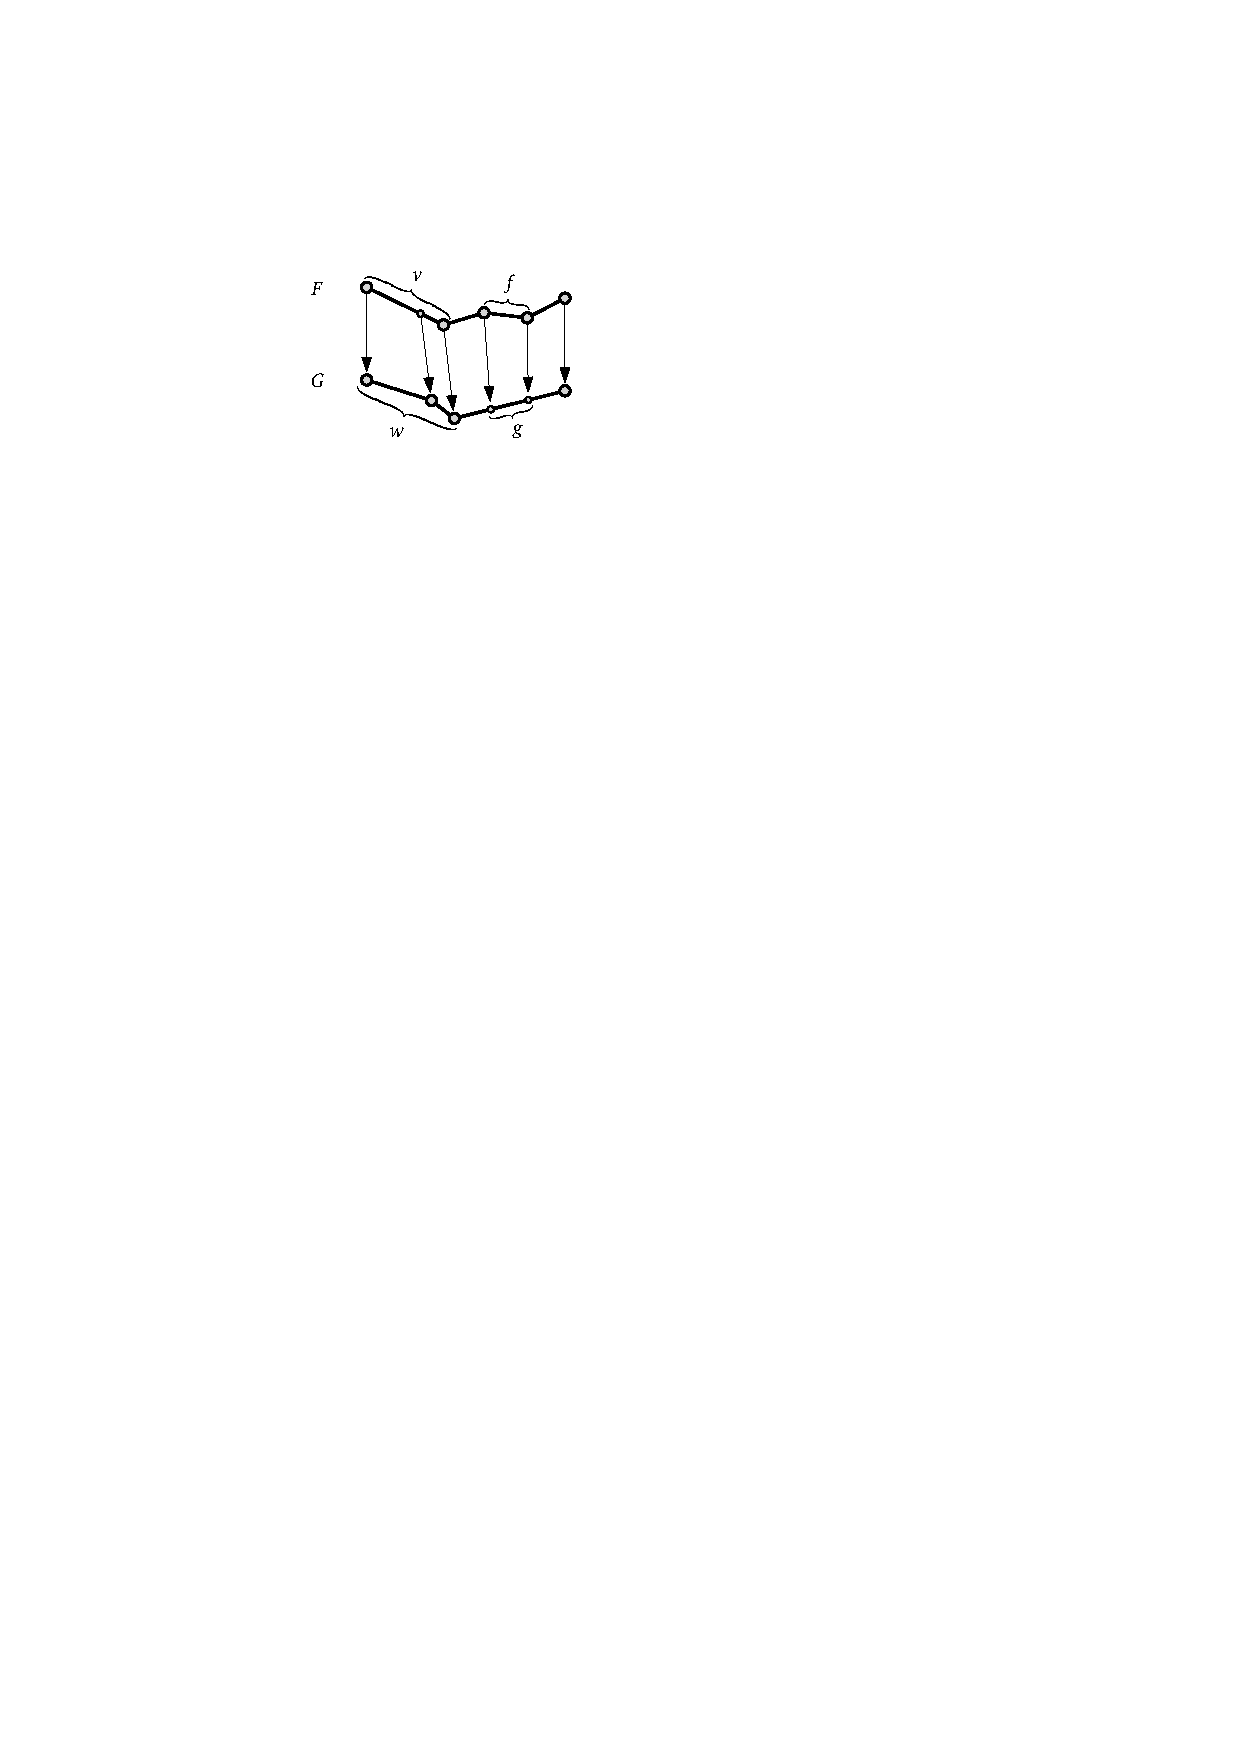
\includegraphics[page=1]{Admin_MorphCorr}
\caption{Corresponding polylines:~$F$ and~$G$,
	corresponding subpolylines:~$v$ and~$w$,
	and corresponding line segments:~$f$ and~$g$.}
\label{fig:Admin_BasicConcepts}
\end{figure}

Let polyline~$F$ on~\ml and polyline~$G$ on~\ms 
be a pair of corresponding polylines. 
Let~$f=\overline{\alpha(0)\alpha(1)}$ 
be a line segment on~$F$, and 
let~$g=\overline{\beta(0)\beta(1)}$ 
be a line segment on $G$ that corresponds to~$f$. 
Let~$\alpha(0)=(x_1,y_1)$, $\alpha(1)=(x_2,y_2)$, 
$\beta(0)=(x_3,y_3)$, and~$\beta(1)=(x_4,y_4)$, 
which are already known. 
The coordinates of a pair of 
corresponding points~$\alpha(u) \in f$ 
and~$\beta(u) \in g$ are
\begin{align}
	\alpha(u)=(1-u)\alpha(0) + u \alpha(1), \nonumber \\
	\beta(u)=(1-u)\beta(0) + u \beta(1). \nonumber 
\end{align}
When we morph~$f$ to~$g$, 
we move each point~$\alpha(u)$ 
to its corresponding point~$\beta(u)$;
see \fig\ref{fig:Admin_Integral_Correspondence}.
We define the cost of this morphing
as the integral over the distances between all the pairs of 
corresponding points, that is,
\[
\delta(f, g)=\int_{0}^{1}|\beta(u) - \alpha(u)|du,
\]
where~$|\beta(u) - \alpha(u)|$ is the Euclidean distance 
between~$\alpha(u)$ and~$\beta(u)$, 
which can be represented as~$\sqrt{au^2+bu+c}$. 
The coefficients~$a$, $b$, and~$c$ are dependent on 
the coordinates of~$\alpha(0)$, $\alpha(1)$, $\beta(0)$, 
and~$\beta(1)$, as follows. 
\begin{align}
a=~&(x_1-x_2-x_3+x_4)^2+(y_1-y_2-y_3+y_4)^2,  \nonumber \\
b=~&-2(x_1-x_3)(x_1-x_2-x_3+x_4) \nonumber \\
&-2(y_1-y_3)(y_1-y_2-y_3+y_4),  \nonumber \\
c=~&(x_1-x_3)^2+(y_1-y_3)^2. \nonumber
\end{align}
Let~$X=au^2+bu+c$. 
We have~$a\geq0$ and, 
since~$X\geq0$ ($X$ is the square of a Euclidean distance), 
$\Delta=4ac-b^2\geq0$. 
Note that, if~$a=0$, then~$b=0$. Let
\[
\delta(f, g)=\int_{0}^{1}|\beta(u) - \alpha(u)|du=\int_{0}^{1}\sqrt{X}du.
\]
Then $\delta(f, g)$ can be computed, according to 
\textcite[p.~1064, 
integrals~241 and~245]{Bronstein2001}, as follows:
\[
\delta(f, g)=\\
\begin{cases}
\sqrt{c}u|_0^1 & \text{if } a=0,\\
\frac{(2au+b)\sqrt{X}}{4a}|_0^1 & \text{if } a>0, \Delta=0,\\
\frac{(2au+b)\sqrt{X}}{4a}|_0^1 + 
\\\frac{\Delta}{8a\sqrt{a}}\ln(2\sqrt{aX}+2au+b)|_0^1 & \text{if } a>0, 
\Delta>0.
\end{cases}
\]

\begin{figure}[tb]
\centering
\includegraphics[page=2]{Admin_MorphCorr}
\caption{Corresponding points of 
a pair of corresponding line segments.}
\label{fig:Admin_Integral_Correspondence}
\end{figure}

Cost~$\delta$ can be regarded as the average distance of 
moving each~$\alpha(u)$ to each~$\beta(u)$.
\fig\ref{fig:Admin_IntegralComputation} 
shows a few examples of computing~$\delta$. 
We obtain the optimum correspondence by
minimizing the cost of moving between corresponding points, 
where the lengths of line segments are used as weights:
\[
\delta(F,G) =
\min_
{\substack
	{\pi \text{: correspondence} \\ 
		\text{between $F$ and $G$}
	}
} 
\sum_
{\substack
	{f\in F \text{ and }g\in G, \\ 
		\text{ where } f \text{ corresponds to } g \text{ in } 
		\pi
	}
}
\frac{|f|+|g|}{2} \delta(f,g).
\]
In other words, there can be many choices of 
defining corresponding points
(see \fig\ref{fig:Admin_ChooseCorrespondence}),
but we choose the one that minimizes cost~$\delta(F,G)$.


\begin{figure}[tb]
\centering
\includegraphics[page=3]{Admin_MorphCorr}
\caption{Examples of computing $\delta(f,g)$. 
The values in the subfigures 
represent the lengths of the edges.}
\label{fig:Admin_IntegralComputation}
\end{figure}

\begin{figure}[tb]
\centering
\includegraphics[page=4]{Admin_MorphCorr}
\caption{Three possible ways of defining corresponding points
	between the two polylines.
	Correspondence $\pi_2$ is the one 
	that minimizes cost~$\delta(F,G)$.
}
\label{fig:Admin_ChooseCorrespondence}
\end{figure}

Recall that \textsc{Optcor} considers three cases of a 
correspondence for an edge. 
We find that the first case, an edge corresponding to a vertex, 
may result in different numbers of vertices 
on the two polylines.  
Our major modification is removing this case 
from the algorithm.
This change ensures that
a pair of corresponding polylines 
will eventually have the same 
numbers of vertices (or line segments).
This property is essential for 
constructing CTs, 
which are used later in our workflow.  
We name our modified version \textsc{Optcor-s}, 
where letter \emph{S} stands for \emph{Simplified}.

Suppose that there are originally~$n_F$ vertices on~$F$ 
and~$n_G$ vertices on~$G$,
\textsc{Optcor-s} requires that 
the look-back parameter~$k$ is bounded from below 
by~$n_F/n_G$ and~$n_G/n_F$. 
Otherwise, there will be at least one segment 
that corresponds to a vertex. 
In our experiments, we always use a (large) value of~$k$ 
that produces results with high quality 
(in the sense of the dynamic-programming algorithm). 
We morph by interpolating between corresponding points using
straight-line trajectories. 
\fig\ref{fig:Admin_MorphCorr} shows an example
with~$0.25$, $0.5$, and~$0.75$ for~$t$.

\begin{figure}[tb]
\centering
\includegraphics[page=5]{Admin_MorphCorr}
\caption{Morphing polyline $F$ to its corresponding 
    polyline $G$. 
    The arrows show the moving trajectories of the vertices.}
\label{fig:Admin_MorphCorr}
\end{figure}

Some other algorithms for computing corresponding points 
can be used (e.g., linear interpolation). 
We observed that an algorithm which
computes corresponding points more carefully 
can yield better results, 
meaning that the interpolated polylines 
are more similar to the two sources and
crossings are less likely introduced.
Some sophisticated algorithms can be 
considered to define the interpolation trajectories, 
such as geodesic shortest paths~\parencite{Bereg2005}, 
b-morphs~\parencite{Whited2011BallMorph}, 
or a method based on 
least squares adjustment~\parencite{Peng2013LSA}. 
Specifically, it is possible to use CTs
not only for the transformation step (as in our method) 
but also to ensure the topological consistency 
in the morphing step~\parencite[see][]
{GotsmanS2001,Surazhsky2003Intrinsic,Surazhsky2004HighQuality}.

%title displays in contents
\subsection[Morphing a Polyline to 
Its Generated Corresponding Polyline] 
{Morphing a Polyline to 
Its Generated Corresponding Polyline \\ During Fade-out}
\label{sec:Admin_MorphSinglePolylines}

For the thinner polylines on~\ml, 
morphing them must be consistent with 
what we do to the thicker corresponding polylines. 
To achieve this, we generate their corresponding polylines, 
that is, thinner polylines on~\ms. 
We transform the thinner polylines on~\ml based on CTs
to get a set of new polylines.
Then, we simplify these new polylines 
to generate the thinner polylines on~\ms,
where we use the Douglas--Peucker algorithm
\parencite{Douglas1973}.

We construct a pair of CTs
for each pair of polygons correspondingly bounded
by the thicker polylines on~\ml and 
the thicker polylines on~\ms
(see \figs\ref{fig:Admin_Introduction}b
and~\ref{fig:Admin_Introduction}e). 
We call them the \emph{triangulation on~\ml} and 
the \emph{triangulation on~\ms}. 
Constructing CTs requires that
the two polygons have the same number of vertices,
which have been attained by using \textsc{Optcor-s}
(see \sect\ref{sec:Admin_MorphCorr}). 
We use the algorithm of \textcite{AronovSS93}
to construct CTs. 
For the two polygons both with $m$ vertices, 
we triangulate them independently
(see \figs\ref{fig:Admin_ConstructCTs}a 
and~\ref{fig:Admin_ConstructCTs}b). 
Then we create a regular~$m$-gon and 
map the chords of the two triangulations 
into the regular~$m$-gon
(see \figs\ref{fig:Admin_ConstructCTs}c). 
The mapped chords may cross with each other.
We use the crossings as dummy vertices and
split the mapped chords
(see \figs\ref{fig:Admin_ConstructCTs}d). 
As a matter of fact, these dummy vertices are called 
\emph{steiner points} \parencite{AronovSS93}.
These split chords may produce some convex faces
(see \fig\ref{fig:Admin_ConstructCTs}d).
We triangulate each convex face
that has more than three vertices. 
To triangulate, we select one vertex and 
add edges between 
this vertex to each of the other vertices, 
except the two immediate-neighboring ones. 
After triangulating, we have 
a \emph{combined} triangulation
(see \fig\ref{fig:Admin_ConstructCTs}e).
We map the combined triangulation 
(including steiner points and new edges)
back to modify the two original triangulations. 
By the modification, we have a pair of 
CTs of the two original polygons
(see \figs\ref{fig:Admin_ConstructCTs}f 
and~\ref{fig:Admin_ConstructCTs}g).

\begin{figure}[tb]
\centering
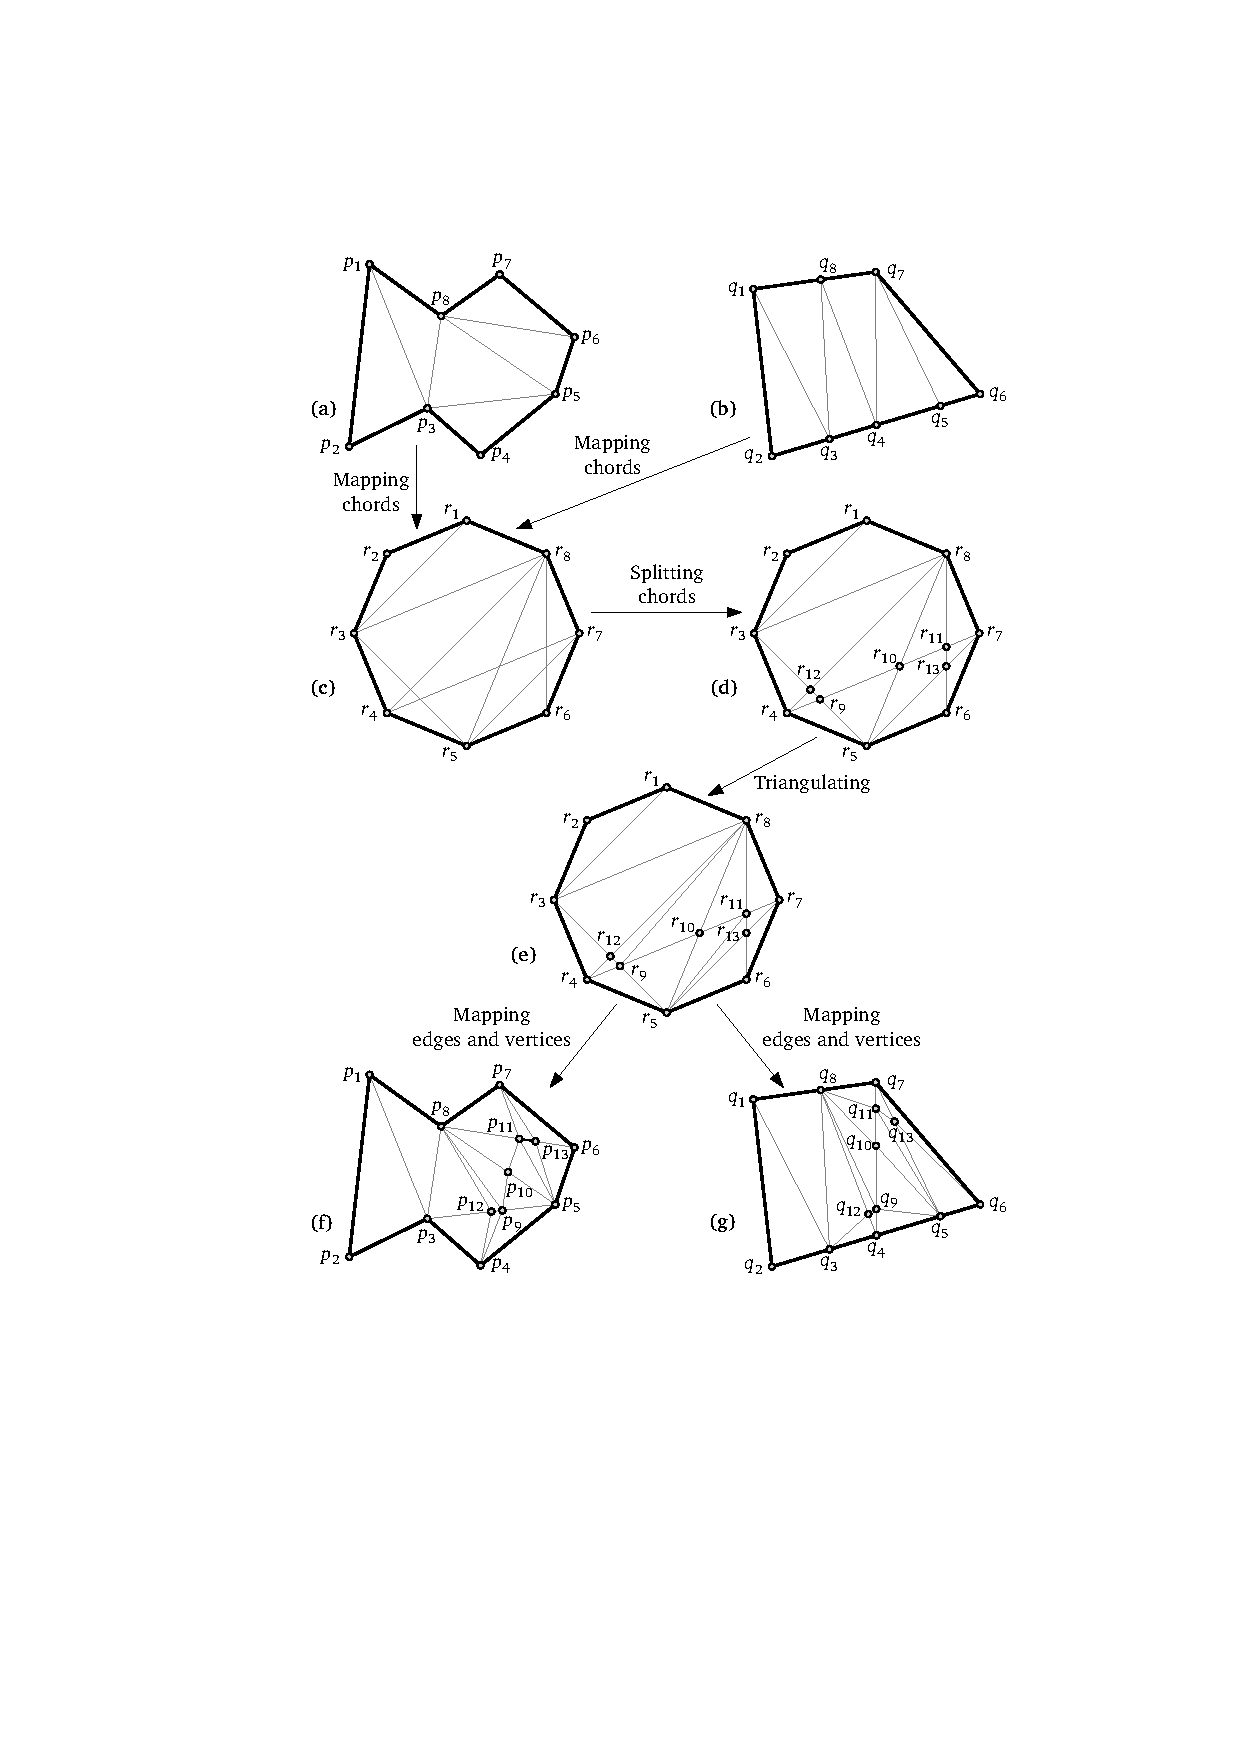
\includegraphics[page=1]{Admin_MorphSingle}
\caption{Constructing compatible triangulations.}
\label{fig:Admin_ConstructCTs}
\end{figure}


With the CTs, 
we transform the thinner polylines in the 
triangulation on~\ml to the polylines on~\ms, 
according to simplicial coordinates. 
The new polylines should traverse exactly the ``same'' 
triangles as thinner polylines on~\ml.
To this end, we compute the crossings 
between thinner polylines and 
the edges of the triangulation; 
then, we also transform these crossings
into the triangulation on~\ms. 
Because of the crossings, the new polylines have
more vertices than the thicker polylines on~\ml. 
While our aim is to generate polylines that have
the same density of vertices as the thicker polylines on~\ms. 
Hence, we simplify the new polylines 
(see \fig\ref{fig:Admin_Introduction}f). 
For a \emph{thinner hole} (polygon) on~\ms, 
we keep at least three vertices during simplification 
to avoid degenerating
it to a straight line or a point.
We call the simplified polylines 
the \emph{thinner polylines on~\ms}.

Again, we use algorithm \textsc{Optcor-s} 
to compute corresponding points
for each pair of corresponding thinner polylines, 
which are respectively on~\ml and~\ms. 
We use straight-line trajectories
to interpolate between corresponding points. 
As the thinner polylines do not exist when~$t=1$, 
we fade them out during the morphing process. 
An example is shown in \fig\ref{fig:Admin_Introduction}c.

\subsection{Running Time}
\label{sec:Admin_Runningtime} 

We analyze the running time for a pair of polygons correspondingly bounded by 
the thicker polylines on~\ml and the thicker polylines on~\ms. 
We use $N$ to denote 
the number of vertices of the polygon on~\ml, 
$n$ the number of vertices of the polygon on~\ms, 
and $N'$ the number of vertices of all the thinner polylines 
inside the polygon on~\ml. 
For simplicity, we assume that $O(N')\in O(N)$.

Constructing the CTs takes time~$O(N\log N + l)$ 
according to \textcite{AronovSS93}, 
where~$O(l)\in O(N^2)$ is the number of steiner points 
inserted during the construction.
Simplifying the polylines resulted from transformation, 
using the Douglas--Peucker algorithm, 
costs time 
$O(N(N+l)\log{N})$~\parencite{Hershberger92speedingup}.  
\textsc{Optcor-s} takes time~$O(k^2Nn)$ 
to compute corresponding points, 
where~$k$ is the look-back parameter. 
Fortunately, outputting the representation at a target scale 
only takes time~$O(N)$.
Therefore, our method is feasible in real time. 
In fact, for each (possibly injected) vertex~$p$ on~$F$ 
we store a representation such as~$p(t)=(1-t)p+tq$,
where~$q$ is the vertex on~$G$ that corresponds to~$p$. 
In our implementation, computing corresponding points
is the by far most time-consuming step.



\section{Case Study}
\label{sec:Admin_CaseStudy}

We implemented our method based on 
C\# (Microsoft Visual Studio~2010) and ArcGIS Engine~10.1. 
We ran our case study under 
Windows~7 on a $3.3\,$GHz dual core CPU with $8\,$GB RAM. 
We measured time consumption based on the
built-in C\# method System.Environment.TickCount.

We tested our method 
on the administrative boundaries of Mainland China
(see \figs\ref{fig:Admin_Data}a and~\ref{fig:Admin_Data}c),
which are from 
the National Fundamental Geographic Information System 
and are based on the projected coordinate system 
\emph{Krasovsky 1940 Lambert Conformal Conic}. 
We removed the enclave in Gansu province 
as well as all the islands.
%
We used county boundaries (see \fig\ref{fig:Admin_Data}a)
and provincial boundaries (see \fig\ref{fig:Admin_Data}c),
where the polylines have been preprocessed
(see \sect\ref{sec:Admin_Preprocessing}).
%
Since we can hardly see the details
if we present the whole map, 
we focus on a small portion, say, 
Tianjin province\footnote{Interactive animations 
of more	provinces are available at \url
{http://www1.pub.informatik.uni-wuerzburg.de/pub/data/agile2016/}.
(We recommend opening the website with Google Chrome.)}
(also known as Tianjin municipality);
see \figs\ref{fig:Admin_Data}b and~\ref{fig:Admin_Data}d.

\begin{figure}[tb]
\centering
\includegraphics{Admin_CaseStudy_Data}
\caption{Administrative boundaries of Mainland China.}
\label{fig:Admin_Data}
\end{figure}

\fig\ref{fig:Admin_CaseStudy} shows our results of Tianjin.
Recall that our aim is to continuously generalize 
from counties~\ml to provinces~\ms. 
According to the provincial boundaries in
\fig\ref{fig:Admin_CaseStudy}c, we are able to
distinguish the hierarchies of the county boundaries in
\fig\ref{fig:Admin_CaseStudy}a 
Then, we find the matched polylines 
(the thicker ones in \figs\ref{fig:Admin_CaseStudy}a 
and~\ref{fig:Admin_CaseStudy}c) and the unmatched polylines 
(the thinner ones in\fig\ref{fig:Admin_CaseStudy}a); see 
step~\circled{1}.

\begin{figure}[tb] 
\centering
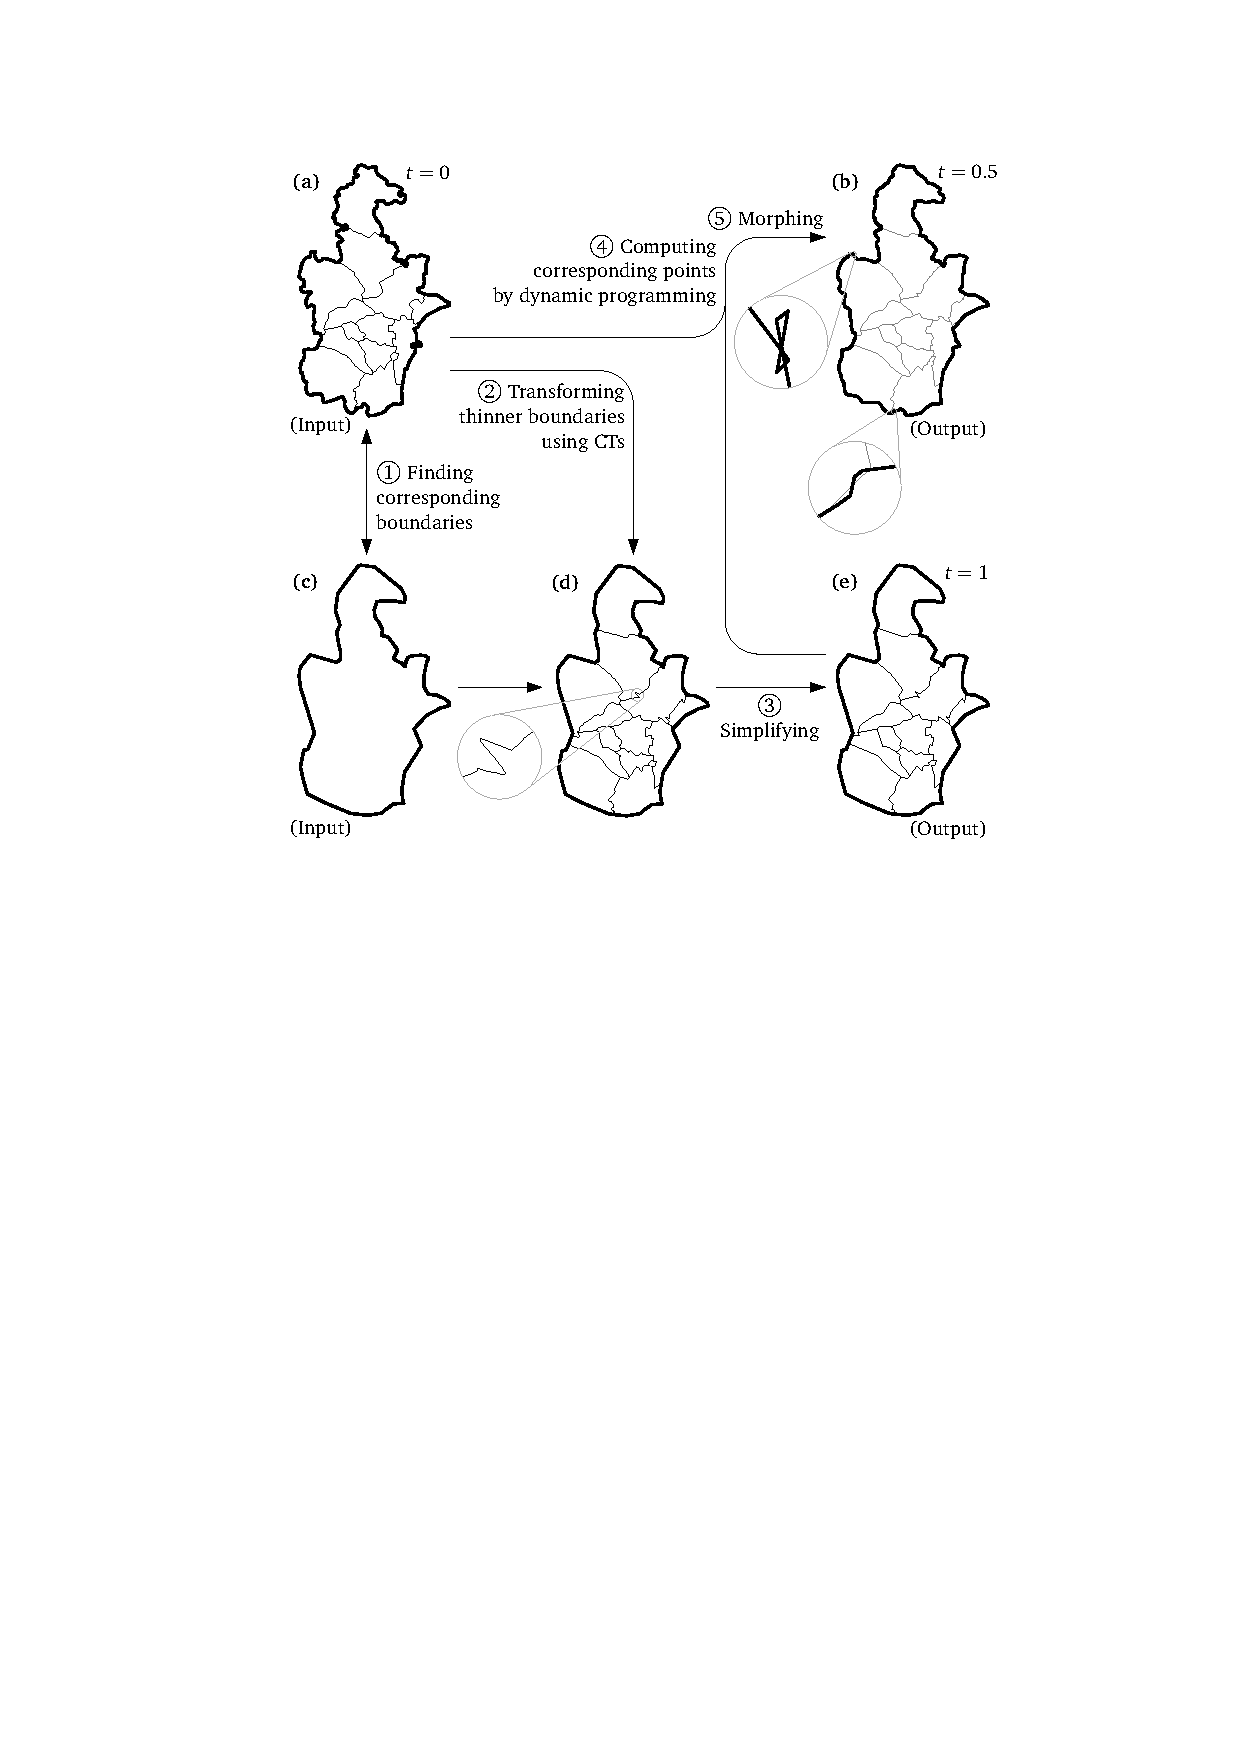
\includegraphics[page=1]{Admin_CaseStudy_Results}
\caption{Case study on administrative boundaries
    of Tianjin province.
	The circled numbers indicate the step orders, 
	analogous to \fig\ref{fig:Admin_Introduction}.     
	For the sake of legibility, 
    we did not display the CTs. 
	Continuous generalization is achieved by 
	morphing from~(a) to~(e).  
	The thinner boundaries in~(b) are being faded out
	during the morphing.}
\label{fig:Admin_CaseStudy}
\end{figure}

In step~\circled{2}, we transform the thinner boundaries in 
\fig\ref{fig:Admin_CaseStudy}a
so that there are corresponding thinner boundaries on~\ms
(see \fig\ref{fig:Admin_CaseStudy}d).
Recall that we compute corresponding points between 
corresponding thicker polylines using \textsc{Optcor-s}
and then transform thinner polylines based on CTs.
When computing corresponding points, 
we used the fact that the~$90$ thicker polylines 
(with~$55{,}533$ vertices) on~\ml and 
the~$90$ thicker polylines (with~$7{,}527$ vertices) on~\ms 
shared many vertices (\ms may be generalized from~\ml).
We split the thicker polylines, on~\ml and~\ms, 
into many subpolylines according to the shared vertices. 
We computed corresponding points for each pair of subpolylines, 
which was much faster than computing without the splitting. 
Using look-back parameter~$145$, 
the computation takes time~$266\,$s 
with cost~$\sum \delta(F,G)=125{,}050\,\mathrm{km}^2$. 
Value~$145$ is the smallest look-back parameter
that achieves the optimum result in
the sense of the dynamic programming algorithm. 
Constructing the CTs costs $168\,$s. 
There is no conflict \mine{for the new polylines} in
\fig\ref{fig:Admin_CaseStudy}d. 
However, a flaw is that there are some zigzags 
caused by our transformation
(see for example the enlarged figure next to 
\fig\ref{fig:Admin_CaseStudy}d)
%
We also tested transforming by the rubber-sheeting method of 
\textcite{Doytsher2001}, 
which, unfortunately, introduced~$39$ crossings. 

In step~\circled{3}, we simplified the thinner polylines 
in \fig\ref{fig:Admin_CaseStudy}d
using the Douglas--Peucker algorithm. 
This simplification took $29\,$s 
and caused~$8$ crossings as well as~$2$ overlaps. 
We corrected the~$10$ conflicts by hand. 
Note that we can avoid these conflicts by using
a topologically consistent line simplification method, 
e.g., the algorithm of \textcite{Saalfeld1999}.

In step~\circled{4}, we use \mbox{\textsc{Optcor-s}} 
to compute corresponding points between 
the~$5{,}819$ thinner polylines 
(with~$438{,}092$ vertices) on~\ml and 
the~$5{,}819$ thinner polylines 
(with~$58{,}105$ vertices) on~\ms.
This time, there are no shared vertices.
The computation took about~$16.5$ hours 
with look-back parameter~$203$, 
where this value was required by 
a pair of corresponding polylines 
to guarantee~$k \geq n_F/n_G$ 
(see \sect\ref{sec:Admin_MorphCorr}).
The cost for the correspondences 
is~$\sum \delta(F,G)=477{,}185\,\mathrm{km}^2$.

In step~\circled{5}, we morph from counties to provinces 
using straight line trajectories. 
We show our continuous generalization of Tianjin in 
\fig\ref{fig:Admin_CaseStudy_Tianjin}.
Generating~$5{,}909$ polylines (with $496{,}106$ vertices) of 
Mainland China at any intermediate scale took about~$1.5\,$s.
Storing these polylines to shapefile format cost about~$45\,$s,
mainly due to the slow creation of polylines in ArcGIS Engine.
Unfortunately, this morphing caused conflicts on the 
intermediate-scale maps; 
two examples are shown in the enlarged figures next to
\fig\ref{fig:Admin_CaseStudy}b. 
For instance, there are~$41$ crossings on the 
intermediate-scale map of Mainland China when~$t=0.5$. 
To avoid these crossings, we can use an algorithm 
that guarantees topological consistency, 
for example, the algorithm of \textcite{GotsmanS2001}.

\begin{figure}[tb]
\centering
\includegraphics[page=2]{Admin_CaseStudy_Results}
\caption{The continuous generalization of Tianjin province.}
\label{fig:Admin_CaseStudy_Tianjin}
\end{figure}


\section{Concluding Remarks}
\label{sec:Admin_Conclusions}

In this chapter, we have shown that rubber-sheeting, 
a popular method for transforming polylines, 
can yield topological conflicts.
Therefore, we turned to transforming based on CTs,
which apparently have not been used 
in GIScience before, 
except by hand~\parencite[e.g.,][]{Fuse2004}.
We have used CTs to 
transform unmatched polylines and 
managed to achieve topological consistency. 
Although computing corresponding points is slow, 
the computed results support 
real-time interactions, e.g., zooming.
Comparing to the rubber-sheeting transformation, 
our method resulted in larger distortions.  
An extreme instance is shown in
\fig\ref{fig:Admin_CT-RS-Comarison-shanghai}.
To decrease the amount of distortion, 
one could try constructing CTs 
that uses the maximum number of chords common to 
both independent triangulations.
To that end, we could extend the dynamic programming algorithm
mentioned by \textcite{Diwan2011Triangulations}.
Whether this idea actually yields better transformation results 
is a question that requires further research.
A similar problem is to minimize the number of steiner points 
when constructing CTs.
This problem is NP-hard for polygons with holes and 
remains open for simple polygons~\parencite{Lubiw2017CT}.

Our current implementation of constructing CTs 
are not able to deal with holes on smaller-scale map~\ms.
Fortunately, \textcite{BabikovSW97} suggested a solution.
We used the Douglas--Peucker algorithm to simplify the
polylines resulted from transformation.  
As expected, this algorithm led to some topological conflicts.
To solve this problem, we may use Saalfeld's variant of the 
Douglas--Peucker algorithm~\parencite{Saalfeld1999}.
In the morphing process, 
we have used straight-line trajectories 
to interpolate between corresponding points.
Again, this interpolation has introduced crossings.
In order to guarantee topological consistency 
in the morphing process,
we can use an algorithm based on CTs
to define the interpolation trajectories, 
e.g., the algorithm of \textcite{GotsmanS2001}. 
With these two replacements, our workflow can
generalize two-level hierarchical subdivisions 
(such as administrative boundaries) 
in a continuous and topologically consistent way.

\begin{figure}[tb]
\centering
\includegraphics[page=3]{Admin_CaseStudy_Results}
\caption{A comparison of the method based on CTs and 
	the rubber-sheeting method 
	for	transforming the thinner polylines on~\ml, 
	using the data of Shanghai as instance. 
	(a)~\ml and the CTs. 
	(b)~\ms and the CTs, where the thinner polylines 
	were transformed from (a) based on CTs.
	(c)~\ms, where the thinner were transformed from (a) 
	by the rubber-sheeting method
	of \textcite{Doytsher2001}.} 
\label{fig:Admin_CT-RS-Comarison-shanghai}
\end{figure}







\chapter %\chapter[<ToC-title>]{<Title>}
%we add "\hspace{0.95mm}~" 
%to make the headline align on the top of the pages 
[Continuously Generalizing 
Buildings to Built-up Areas\hspace{0.95mm}~\\
by Aggregating and Growing]
{Continuously Generalizing\\ 
	Buildings to Built-up Areas\\
	by Aggregating and Growing}
\label{chap:Bldg}


Digital multi-scale maps such as Google Maps and OpenStreetMap 
support zooming by displaying maps at different levels. 
This discrete strategy may result in sudden changes, 
which disturb user navigation.
To provide better zooming experience, 
we try to produce a sequence of maps 
with small incremental changes 
from a level to another level.
This process is known as \emph{continuous generalization}.

A way to achieve continuous generalization is to use morphing.
Often, a start map (at a larger-scale) and 
a goal map (at a smaller-scale) 
are used as input, 
then maps at intermediate scales are produced 
while the start map is morphed to the goal map.
In order to morph, correspondences 
between two maps need to be defined.
For example, corresponding points 
between a pair of polylines have been investigated based on 
dynamic programming \citep{Noellenburg2008}, 
Delaunay triangulations and binary line generalized tree 
(BLG-tree) \citep{Deng2015},
and simulated annealing \citep{Li2017Annealing}.
From a point to its corresponding point,
a straight-line trajectory is often used to interpolate.
\citet{Peng2013LSA} defined trajectories 
based on least-square adjustment 
in order to obtain more reasonable intermediate-scale polylines.
Using morphing, \citet{Peng2016Admin} continuously generalized 
administrative boundaries based on compatible triangulations. 
When the numbers of line features are different 
on the start and goal maps, 
a continuous selection is required; 
\citet{Chimani2014Eat} proposed to generate a 
removing sequence applicable for road network.
They removed one road at each step
while keeping the remaining roads connected.

These methods are interesting but only work on lines. 
Our problem of building polygon interpolation 
cannot be achieved by similar morphings. 
Regarding the continuous generalization of polygon features,
\citet{Danciger2009} grew polygons during zooming out. 
Their method preserves polygons' 
topology, area-ratios, and relative positions.  
In the case where the goal map is an aggregated version of 
a start land-cover map, 
\citet{Peng2017AStar} computed optimal sequences 
for aggregating land-cover areas.

Buildings are important elements on maps. 
Many methods have been proposed to generalize them 
but not necessarily in a continuous way.
For example, \citet{Haunertwolff2010Building} simplified a set 
of buildings based an integer program.
Their simplification minimizes the number of total edges and guarantees that the errors are smaller than 
a user-defined tolerance.
At the same time, their method does not introduce any topological conflict.
\citet{Buchin2011_Simp} simplified buildings based on 
edge-move operations.
Their method preserves orientations of the edges.

When users zoom out on digital maps, 
buildings become smaller and 
the distances between them decrease. 
In addition to simplifying the buildings,
we also need to aggregate them when they become close  \cite{Weibel1997}. 
Several methods were proposed 
to aggregate buildings while preserving their shape 
(e.g., right angles) 
\citep{Regnauld2001,RegnauldRevell07,Damen2008}. 
These algorithms can be used as inspirations 
to define a continuous transformation of buildings.

Algorithms were also proposed to create 
built-up areas (that appear on our goal map) from 
individual buildings (that appear on our start map). 
For instance, \citet{Chaudhry2008} identified 
the boundaries of urban settlement 
by calculating `citiness' based on buildings. 
However, this method cannot be adapted 
to provide a continuous transformation 
from buildings to built-up areas.

Finally, some papers directly tackle 
the continuous transformation of buildings 
when scale is reduced. 
\citet{Li2017_Building} morphed between two buildings 
at different scales.
They managed to preserve the orthogonal characteristics of 
buildings, but their algorithm cannot be used in our case 
as our goal map does not contain buildings anymore.
\citet{Touya2017Progressive} 
transformed buildings into built-up areas, 
where they progressively replaced buildings 
by the shape of the blocks to which the buildings belong. 
However, this last algorithm is not continuous enough 
because each iteration directly transforms 
a set of buildings in a block to a polygon 
that covers the whole block. 
As a result, there is no existing solution 
for the continuous generalization of buildings 
into built-up areas.


Our contributions are as follows.
In \sect\ref{sec:Methodology},
we continuously generalize a start map of buildings
(at a larger scale) 
to a goal map of built-up areas (at a smaller scale).
The generalization consists of 
aggregating, growing, and simplifying.
We aggregate the original buildings which will be too close 
at an output scale by adding bridges.
We grow (bridged) original buildings by buffering,
where we use so-called \emph{miter} joins to keep the right 
angles of buildings.
Because of using this kind of joins 
instead of \emph{round} ones,
we have new problems.
We show how to solve these problems.
We also simplify the buildings according to output scales.
Finally, we analyze running time at the end of this section.
We carry out a case study 
and discuss the performances of our method in 
\sect\ref{sec:CaseStudy}.
We conclude this chapter in \sect\ref{sec:Conclusion}.

\section{Methodology}
\label{sec:Methodology}
The input map is our start map.
We denote the scale of the start map by~$1:M_\mathrm{s}$.
We generate the goal map at scale~$1:M_\mathrm{g}$ 
($M_\mathrm{g} > M_\mathrm{s}$) by generalizing the start map. 
We use time~$t\in[0,1]$ to define 
the process of continuous generalization. 
We require that 
the generalization yields exactly the start map when~$t=0$ 
and the goal map when~$t=1$.
The start map should be continuously changed to the goal map 
when~$t$ increases from~$0$ to~$1$.
For the sake of convenience, we define 
\emph{scale denominator}~$M_t= 
M_\mathrm{s} + t \cdot (M_\mathrm{g}-M_\mathrm{s})$.

We carry out the continuous generalization 
by growing the original buildings. 
If some grown buildings become too close at time~$t$,
we aggregate the related original buildings by adding bridges.
We grow the (bridged) original buildings 
by buffering with miter joins.
At any time $t$, the grown buildings 
need to be simplified to look like buildings.
This simplification is carried out in two steps:
the first one is to use dilating and eroding 
to remove ``dents'' and ``bumps''; 
the second step is to remove vertices 
using the algorithm of Imai and Iri \citep{ImaiIri1988}.
To make sure that buildings never shrink 
when~$t$ is increasing,
we merge the shape of a building at time~$t$ 
and its shape at the preceding time (before~$t$). 
We clip the buildings using the shape on the goal map to 
ensure that the buildings will not 
grow out of the intended built-up areas.
\fig\ref{fig:Bldg_Framework} shows 
the framework of our method;
we explain the presented operators
in the following subsections.




\begin{figure}[tb]
\centering
\includegraphics[page=1]{Bldg_Framework}
\caption{The framework of our method.}
\label{fig:Bldg_Framework}
\end{figure}


\subsection{Growing buildings by buffering}
\label{sec:Grow}
We denote by $d_\mathrm{G}$ 
the \emph{growing distance} for the goal map.
At time $t$, the distance is
\begin{equation}
\label{eq:d_Gt}
\dtrm{G} = t \cdot d_\mathrm{G}.
\end{equation}

There are three typical joins when buffering a polygon, i.e.,
round, miter, and square joins
(see \fig\ref{fig:Buffer_ThreeKinds}).
We choose the miter joins to grow buildings in order to
preserve right angles.
If an angle is acute, however, 
an excessively long \emph{spike} will be produced.
This spike may go across other buildings 
(see for example \fig\ref{fig:Buffer_MiterLimits}a).
To avoid this kind of interruptions, 
we require that if the tip of a spike 
is more than $\alpha \dtrm{G} (\alpha \ge 1)$
away from the original vertex, 
then we apply a \emph{square} join
(see \fig\ref{fig:Buffer_MiterLimits}b).
To keep right angles of buildings, 
we must have \emph{miter limit}~$\alpha \geq \sqrt{2}$. 
We set $\alpha  = 1.5$. 
In this case, a square join will be applied 
when an angle is smaller (more acute) than $83.6 \degree$.

\begin{figure}[tb]
\centering
\includegraphics[page=1]{Bldg_Buffering}
\caption{Three ways of buffering a polygon and 
	their applications.}
\label{fig:Buffer_ThreeKinds}
\end{figure}

\begin{figure}[tb]
\centering
\includegraphics[page=2]{Bldg_Buffering}
\caption{Using square joins instead of miter joins to avoid
    long spikes.
}
\label{fig:Buffer_MiterLimits}
\end{figure}




\subsection{Simplifying grown buildings based on dilating and 
eroding}
\label{sec:DilationErosion}
As mentioned earlier, 
methods of simplifying building have already been well studied. \citet{Damen2008} generalized buildings using 
morphological operators.
A drawback of their method is that the orientation of the 
buildings have to be identified.
\citet{Meijers2016} simplified buildings 
using offset curves generated based on straight skeletons.
Our method is similar to \citet{Meijers2016}.
We dilate and erode the buildings to remove dents and 
bumps that can occur when buildings grow
(see \fig\ref{fig:RemoveDentAndBump}).

\begin{figure}[tb]
\centering
\includegraphics[page=1]{Bldg_DilationErosion}
\caption{Removing dents and bumps 
	by dilating and eroding with distance~$d$.
}
\label{fig:RemoveDentAndBump}
\end{figure}

At time~$t$, we should grow buildings with distance~$\dtrm{G}$.
In order to simplify the grown buildings, 
we further dilate them with distance $\dtrm{D}$ ($\dtrm{D}>0$),
erode with $\dtrm{D}+\dtrm{E} (\dtrm{E}>0)$,
and dilate back with $\dtrm{E}$.
A problem of this process is that 
a building may be split into several parts by eroding
(see \fig\ref{fig:ErosionBreak} for example).
The reason is that 
some parts of a building may be increased (by growing and 
dilating) 
with distance $\dtrm{G}+\dtrm{D}$, 
but can be decreased (by eroding) as much as $\alpha 
(\dtrm{D}+\dtrm{E})$.
If $\dtrm{G}+\dtrm{D} < \alpha (\dtrm{D}+\dtrm{E})$ 
and the building is not thick enough, 
a thin part may disappear
(see \fig\ref{fig:ErosionBreak} when using distance~$d_2$).
In order to avoid this problem, we require that
\[
\dtrm{G} + \dtrm{D} \ge \alpha (\dtrm{D}+\dtrm{E}),
\]
which means
\begin{equation}
\label{eq:d_DtBound}
\dtrm{D} \le \frac{\dtrm{G}-\dtrm{E}}{\alpha - 1}.
\end{equation}

\begin{figure}[tb]
\centering
\includegraphics[page=2]{Bldg_DilationErosion}
\caption{Dilating and eroding a polygon 
	with distances~$d_1$ and~$d_2$, where $d_1 < d_2$.
	The result of using~$d_1$ 
	is the same as the original polygon,
	while the result of using~$d_2$
	become two polygons.
}
\label{fig:ErosionBreak}
\end{figure}

We would like to use $\dtrm{E}=\frac{l}{2} \cdot M_t$ so that
any dents and bumps narrower than $l$ will be removed. 
We set~$l=0.3\,\mathrm{mm}$ on map, 
which was used as a length threshold by, for example, 
\citet{Regnauld2001}.
Unfortunately, distance $\dtrm{G}$ can be arbitrarily small 
according to \eq\ref{eq:d_Gt}, 
but $\dtrm{E}$ is at least $\frac{l}{2} M_\mathrm{s}$. 
When time~$t$ is small, $\dtrm{G}-\dtrm{E} \le 0$, 
which violates \eq\ref{eq:d_DtBound}, where $\dtrm{D}>0$.
To mediate this violation, we set eroding distance
\begin{equation}
\label{eq:d_Et}
\dtrm{E} =t \cdot \frac{l}{2} M_\mathrm{g}.
\end{equation}
%Still, we should make sure that $\dtrm{G}-\dtrm{E} > 0$, which 
%means
%$t \cdot \frac{\lambda}{2}\sqrt{a} (M_\mathrm{g}-M_\mathrm{s})-
%t \cdot \frac{l}{2} M_\mathrm{g} >0$.
Still, we have to make sure that $\dtrm{G}-\dtrm{E} > 0$, which 
means
$t \cdot d_\mathrm{G} - t \cdot \frac{l}{2} M_\mathrm{g} >0$.
As a result, we need to make sure that
\begin{equation}
\label{eq:S_g}
M_\mathrm{g} < \frac{2 d_\mathrm{G}}{l}.
\end{equation}

When we grow a bridged building,
a ``bay'' may appear (see \fig\ref{fig:RemoveBay}b).
We remove such a bay by dilating (see \fig\ref{fig:RemoveBay}c)
and then eroding (see \fig\ref{fig:RemoveBay}d) with distance 
$\dtrm{D}$.
We define the width of a bay as the diameter of the largest 
circle 
that can be placed in the bay.
If the width of a bay is smaller than $2\dtrm{D}$, 
then the bay can be removed by dilating with distance 
$\dtrm{D}$.
We wish to remove bays 
which have widths less than~$2 r_\mathrm{h}$.
Variable~$r_\mathrm{h}= 2\sqrt
{ a_\mathrm{h}/ \pi }$
is the radius of a hole 
which is just large enough to be presented on map.
Following \citep{Chaudhry2008}, 
we set area~$a_\mathrm{h} = 8\,\mathrm{mm}^2$ on map.
Sometimes, our~$\dtrm{D}$ is not large enough to remove a bay 
with width~$r_\mathrm{h}$
because of the limitation from \eq\ref{eq:d_DtBound}.
Therefore, we define
\begin{equation}
\label{eq:d_Dt}
\dtrm{D} =\min (\frac{\dtrm{G}-\dtrm{E}}{\alpha - 1}, 
r_\mathrm{h} M_t) .
\end{equation}


\begin{figure}[tb]
\centering
\includegraphics[page=3]{Bldg_DilationErosion}
\caption{Removing a bay by dilating and eroding.
	(a) An aggregate from adding bridges 
	(see \sect\ref{sec:Aggregate}).
	(b) Growing the aggregate with 
	distance~$\dtrm{G}$,
	where the region marked by the dashed circle is a bay.
	(c) Dilating the grown building with~$\dtrm{D}$.
	(d) Eroding the dilated building with~$\dtrm{D}$.
}
\label{fig:RemoveBay}
\end{figure}


\subsection{Iteratively aggregating close buildings by adding 
bridges}
\label{sec:Aggregate}


We grow each original building and, as illustrated in 
\sect\ref{sec:DilationErosion}, simplify the grown building.
If some buildings become too close after these operations,
we aggregate them by adding bridges
(see for example \fig\ref{fig:GrowAndBridge}).
Following \citet{Stoter2009}, 
we define that two buildings are too close if their distance is 
less than
$\varepsilon= 0.2\,\mathrm{mm}$ on map.
The real separation threshold at time $t$ is
\begin{equation*}
\label{eq:d_epsilont}
d_{\varepsilon, t} = \varepsilon \cdot M_t.
\end{equation*}

\begin{figure}[tb]
\centering
\includegraphics[page=1]{Bldg_Aggregating}
\caption{Aggregating original buildings 
	that will become too close at a certain time 
	by adding bridges;
	then, growing the bridged buildings.}
\label{fig:GrowAndBridge}
\end{figure}

Our way of detecting close buildings is simple.
We buffer buildings with distance 
$\left. d_{\varepsilon,t}\middle/2 \right.$
using round joins
(see \fig\ref{fig:Buffer_ThreeKinds});
then, we merge the buffers that intersect with each other.
On this basis, 
the original buildings intersecting with the same merged buffer 
are identified as a group of close buildings.
For each pair of the original buildings in the same group,
we connect them by adding a line segment 
linking the pair of nearest points.
There can be many line segments, 
and they may cross each other or even intersect with buildings.
To make the topology simple, 
we select only some of the line segments as \emph{bridges}.  
If we consider each building as a node and 
each line segment as an edge, 
then we have a graph.
Using Prim's algorithm \citep{Prim1957}, 
we find a minimum spanning tree (MST) in the graph,
using the lengths of the line segments as the weights.
As a result, we use the line segments 
that corresponds to the edges in the MST as bridges.
We aggregate the group of original buildings 
by adding these bridges.

Aggregated and grown buildings may become too close 
because of the additional bridges,
so we have to iterate the aggregation process.
\fig\ref{fig:BridgeMoreBuilding} shows such an example.
We grow and buffer buildings~$p$, $q$, and~$r$.
As the buffers of~$q$ and~$r$ intersect
(see \fig\ref{fig:BridgeMoreBuilding}c),
we aggregate buildings~$q$ and~$r$ by adding a bridge
(see \fig\ref{fig:BridgeMoreBuilding}d).
There are two buildings left in 
\fig\ref{fig:BridgeMoreBuilding}d:
an original one and an aggregate.
We then grow and buffer the two buildings in 
\fig\ref{fig:BridgeMoreBuilding}d, 
the buffer of building~$p$ intersects with
the buffer of the bridge of buildings~$q$ and~$r$
(see \fig\ref{fig:BridgeMoreBuilding}f).
Finally, we aggregate building~$p$ with bridged~$q$ and~$r$
(see \fig\ref{fig:BridgeMoreBuilding}g), 
and there is only one building left in 
\fig\ref{fig:BridgeMoreBuilding}g.
Then, we grow and buffer again 
to get the final shape of the group.
As the number of buildings 
does not decrease from \fig\ref{fig:BridgeMoreBuilding}g
to \fig\ref{fig:BridgeMoreBuilding}i,
we stop the iteration.

When buildings are grown and aggregated iteratively, 
bridges have been added. 
These bridges have a width of~$2\dtrm{G}$ at time~$t$.
This setting guarantees that no bridge is thin when~$t=1$.
As we aggregated all the buildings that will become too close, 
all the separation distances 
between each pair of buildings (or aggregates) 
are larger than distance~$d_{\varepsilon, t}$.
Specifically, if a group of buildings 
will be aggregated at time~$t=1$, 
we say that these buildings are in the same \emph{goal group}. 

\begin{figure}[tb]
\centering
\includegraphics[page=2]{Bldg_Aggregating}
\caption{Iteratively aggregating close buildings 
	by adding bridges.
}
\label{fig:BridgeMoreBuilding}
\end{figure}

\subsection{Simplifying buildings using the Imai--Iri algorithm}
\label{sec:ImaiIri}

When the scale is decreasing ($M_t$ increasing), 
we should remove more and more details. 
So, we simplify the (aggregated) grown buildings
using the Imai--Iri algorithm \citep{ImaiIri1988}.
First, this algorithm finds 
all the valid shortcuts of a polyline.
A shortcut is valid for a segment 
if the distance between the segment and the shortcut 
is at most a specified value
(see \fig\ref{fig:ImaiIri_Shortcut}).
We set the value also as~$l=0.3\,\mathrm{mm}$ on map
(see \sect\ref{sec:DilationErosion}). 
That is, at time~$t$, the distance threshold is
\begin{equation}
\label{eq:d_lt}
d_{l,t}= l \cdot M_t.
\end{equation}
Second, the algorithm finds a sequence of valid shortcuts
using breadth-first search.
The sequence of valid shortcuts 
is an approximation of the polyline 
and has the least number of line segments, 
with error smaller than~$d_{l,t}$.

\begin{figure}[tb]
\centering
\includegraphics[page=1]{Bldg_Shrinking}
\caption{Valid and invalid shortcuts 
	for the Imai--Iri algorithm.
	Parameter~$l$ is the tolerance for errors.}
\label{fig:ImaiIri_Shortcut}
\end{figure}

In order to adapt the Imai--Iri algorithm to our problem,
we add two more constraints for a shortcut to be valid. 
One is that a shortcut must be 
completely inside the grown building.
If a shortcut is outside,
we may not be able to arrive at the shortcut by growing.
The other constraint is that 
a shortcut is not allowed to intersect with
the resulting building at the previous time frame.
We add this constraint 
to avoid the building to shrink.

The classical way of simplifying
a polyline or a polygon is using 
the Douglas--Peucker algorithm \citep{Douglas1973}. 
However, it cannot simplify the shapes enough in our case.
This is why we choose the Imai--Iri algorithm.


%
%
%\subsection{Generating the goal shapes of buildings}
%\label{sec:Goal}
%To generate the goal shapes of buildings, we set time $t=1$.
%We aggregate original buildings (see \sect\ref{sec:Aggregate}).
%Then we grow (see \sect\ref{sec:Grow}) 
%and simplify 
%(see \sects\ref{sec:DilationErosion} and~\ref{sec:ImaiIri}) 
%the 
%grown 
%buildings.
%See for example \fig\ref{fig:GrowAndBridge}, 
%the building at time $t=1$ is the goal shape of the three 
%original buildings.
%
%


\subsection{Generating buildings on intermediate-scale maps}
\label{sec:Unite}

Both the eroding and the line simplification 
may result in a building to be shrunk.
\fig\ref{fig:Shrink_Erosion} and 
\fig\ref{fig:Shrink_Simplification} show such 
examples, respectively.
To avoid these kinds of shrinking,
for a building, we merge its shape at time $t$ 
and its shape at the preceding time (before~$t$). 
For example, we generate a sequence of~$10$ maps,
which means~$t \in \{0.1, 0.2, \dots, 1\}$.
\fig\ref{fig:Shrink_Erosion}c shows the result at~$t=0.6$.
In \fig\ref{fig:Shrink_Erosion}f, 
the darker gray piece is included in the result at~$t=0.6$
but not in the result at~$t=0.7$.
In other words, the result at~$t=0.7$ 
shrinks at the darker gray part.
To prevent this shrinking, 
we merge the result at~$t=0.7$ with 
the result at the preceding time, i.e., $t=0.6$.
The merged result is shown in \fig\ref{fig:Shrink_Uniting}a.
Similarly, \fig\ref{fig:Shrink_Uniting}b shows the merged 
result of buildings 
in \fig\ref{fig:Shrink_Simplification}c 
and~\fig\ref{fig:Shrink_Simplification}h.
This merge also avoids bridges' shrinking;
\fig\ref{fig:BridgeDisappearing} shows such an example.

\begin{figure}[tb]
\centering
\includegraphics[page=2]{Bldg_Shrinking}
\caption{A building shrinks because of dilating and eroding, 
	where~$t_1=0.6$ and~$t_2=0.7$.
	The gray polygons in~(a) and~(d) 
	represent the original building.
	The transparent polygon in~(a) is from 
	growing and dilating the original building with 
	distances~$\dtrm[1]{G}$ and~$\dtrm[1]{D}$.
	The transparent polygon in~(d) is obtained analogously
	as in~(a).
	The darker gray piece in~(f) shows 
	the part which is included in the polygon of~(c) 
	but not in the polygon of~(f).
}
\label{fig:Shrink_Erosion}
\end{figure}


\begin{figure}[tb]
\centering
\includegraphics[page=3]{Bldg_Shrinking}
\caption{A building shrinks because of line simplification, 
	where~$t_1=0.7$ and~$t_2=0.8$.
	The gray polygons in~(a) and~(e) 
	represent the original building.
	The transparent polygon in~(a) is from 
	growing and dilating the original building with 
	distances~$\dtrm[1]{G}$ and~$\dtrm[1]{D}$.
	The transparent polygon in~(e) is obtained 
    analogously as in~(a).
	Note that distances~$d_{l,t_1}<d_{l,t_2}$ 
	(see \eq\ref{eq:d_lt});
	this is why the Imai--Iri algorithm does not 
	remove any vertex of the polygon in~(c)
	but removes two vertices of the polygon in~(g).
	The darker gray pieces in~(h) are 
	the parts which are included in the polygon of~(d) 
	but not in the polygon of~(h).
}
\label{fig:Shrink_Simplification}
\end{figure}

\begin{figure}[tb]
\centering
\includegraphics[page=4]{Bldg_Shrinking}
\caption{Merging a polygon with the polygon 
	at the preceding time.
	(a) Merging the transparent polygons in 
	\figs\ref{fig:Shrink_Erosion}c and~\ref{fig:Shrink_Erosion}f.
	(b) Merging the transparent polygons in 
	\figs\ref{fig:Shrink_Simplification}d 
    and~\ref{fig:Shrink_Simplification}h.
}
\label{fig:Shrink_Uniting}
\end{figure}

\begin{figure}[tb]
\centering
\includegraphics[page=5]{Bldg_Shrinking}
\caption{Avoiding shrinking resulted by moved bridges,
	where~$t_1=0.5$ and~$t_2=0.6$.
	(a) Original buildings.
	(b) Growing buildings with distance~$\dtrm[1]{G}$ and 
	dilating with~$d_{\varepsilon,t_1}/2$;
	buildings~$p$ and~$q$ are identified as in the same group.
	(c) Aggregating~$p$ and~$q$	by adding a bridge.
	(d) Growing the (bridged) buildings in (c)
	with distance~$\dtrm[1]{G}$.
	(e) Growing original buildings with 
	distance~$\dtrm[2]{G}$ and 
	dilating with~$d_{\varepsilon,t_2}/2$;
	all the three buildings are in the same group.
	(f) Aggregating	by adding bridges according to the MST.
	(g) Growing the bridged building in~(f)
	with distance~$\dtrm[2]{G}$. 
	The bridge in~(d) shrinks comparing to~(g).
	(h) Avoiding this shrinking at time~$t_2$ 
	by merging buildings in~(d) and~(g).
}
\label{fig:BridgeDisappearing}
\end{figure}

%\begin{figure}[tb]
%	\centering
%	\includegraphics{Bldg_NearestPoints}
%	\caption{The nearest points between a pair of buildings	
%		change because of growing. 
%		The two squares and the two circles respectively mark
%		the nearest points before and after growing.
%	}
%	\label{fig:NearestPoints}
%\end{figure}

Added to this shrinking problem, 
a building aggregate on an intermediate map should never leave
the goal shape of the aggregated building. 
Otherwise, the building will need to shrink 
to achieve the goal shape.
To avoid shrinking, 
we clip the building using the goal shape 
and remove the parts outside.


\subsection{Eliminating small buildings and small holes}
\label{sec:Eliminate}
Following the previous steps may result in 
some small isolated building aggregates.
We should remove these small aggregates during
the continuous generalization 
because they become too small to be visible at some point.
Therefore, we eliminate a building aggregate if its area is 
smaller than a threshold.
Following \citet{Stoter2009,Chaudhry2008}, 
we set this threshold to~$a=0.16\,\mathrm{mm}^2$ on map.
The real threshold at time~$t$ is
\[
a_t=a\cdot M_t^2.
\]
For the buildings in the same goal group 
(see the definition in \sect\ref{sec:Aggregate}),
we consider the total area of all the buildings at time $t$, 
instead of considering each building individually.

As mentioned in \sect\ref{sec:DilationErosion}, 
we remove holes that have area less than 
$a_\mathrm{h} = 8\,\mathrm{mm}^2$ on map.
The real area threshold for a hole at time $t$ is
\[
a_{\mathrm{h},t}=a_\mathrm{h}\cdot M_t^2.
\]

\subsection{Running time}
Suppose that our input has $n$ edges in total.
Operations like growing, dilating, 
eroding, merging, and clipping 
cost time $O(n^2)$ \citep{Greiner1998Clipping,Palfrader2015}.
We iteratively aggregate in \sect\ref{sec:Aggregate}.
In the worst case, we need to repeat $O(n)$ times,
which increases our running time to $O(n^3)$.
It is unlikely that we need to repeat the aggregation more than 
twice, though.
Simplifying polygons using the Imai--Iri algorithm takes time
$O(n^3)$.
The improved version of the Imai--Iri algorithm by 
\citet{Chan1996} does not help in our case
because we have more constraints when simplifying
(see \sect\ref{sec:ImaiIri}).
As a result, the running time of our method is in $O(n^3)$.


\section{Case Study}
\label{sec:CaseStudy}
We have implemented our method based on
C\# (Microsoft Visual Studio 2015) and ArcObjects SDK 10.4.1. 
The code is available in open source on 
Github\footnote{\url{
https://github.com/IGNF/ContinuousGeneralisation}}.
The offsetting function and clipping function 
are available from library \textsc{Clipper} of 
\citet{Johnson2014}, which is based on the clipping algorithm of
\citet{Vatti1992Clip}.
The offsetting function is used for the buffering, dilating, 
eroding, and merging operations.
We ran our case study under~64-bit 
Windows~7 on a~$3.3\,$GHz dual core CPU with~$8\,$GB RAM.
We measured processing time by the built-in C\# class 
\emph{Stopwatch}.
Our testing data is extracted from a dataset produced 
by the French Mapping Agency (IGN);
see \fig\ref{fig:Data}.
The data is at scale~$1:15{,}000$, 
which means~$M_\mathrm{s}=15{,}000$.
It represents the buildings of four towns, 
i.e., Aussevielle, Denguin,  Poey-de-Lescar, and Siros, 
in the Pyr\'en\'ees-Atlantiques county, south-western France.
IGN also stores a dataset at scale~$1:50{,}000$.
This dataset was obtained mostly
from the data at scale~$1:15{,}000$ 
by buffering with distance~$25\,\mathrm{m}$,
where sometimes distance~$50\,\mathrm{m}$ was also used
in order to identify towns.
A restriction for the town from \citet{Boffet2000} is that 
the longest edge in an MST of the buildings 
should be shorter than~$100\,\mathrm{m}$.

\begin{figure}[tb]
\centering
\includegraphics[page=1]{Bldg_CaseStudy_DataAndResults}
\caption{Data for our case study, at scale~$1:15{,}000$.
	There are $2{,}590$ buildings, 
	which in total have $19{,}255$ edges and have area
	$448{,}802.3\,\mathrm{m}^2$.}
\label{fig:Data}
\end{figure}

We set our goal scale to~$1:50{,}000$, 
which means scale denominator~$M_\mathrm{g}=50{,}000$,
and growing distance~$d_\mathrm{G}=25\,\mathrm{m}$
so that we can compare our result with the existing data.
Also, this setting makes \eq\ref{eq:S_g} hold, 
where error tolerance~$l=0.3\,\mathrm{mm}$.
In \eq\ref{eq:d_Dt}, the first part is always smaller than 
the second part because of our settings.
As a result, dilating distance~$\dtrm{D}=t\cdot 35\,\mathrm{m}$, 
where eroding distance~$\dtrm{E}=t\cdot 7.5\,\mathrm{m}$ 
according to \eq\ref{eq:d_Et} and miter limit~$\alpha=1.5$.

Our program took~$93.6\,\mathrm{s}$ 
to compute the goal shapes of the built-up areas.
The~$56$ built-up areas have~$2{,}095$ edges before line 
simplification.
Using the Imai--Iri algorithm, we have~$1{,}102$ edges left.
In comparison, there are~$1{,}597$ edges left 
when we simplified using the Douglas--Peucker algorithm.

\fig\ref{fig:Bldg_GoalShape} shows 
the bridged original buildings as well as the goal shapes.
We produced a sequence of~$10$ maps,
i.e.,~$t \in \{0.1, 0.2, \dots, 1\}$.
This production cost~$668.2\,\mathrm{s}$ in total.
We show such a sequence of maps in 
\fig\ref{fig:ContinuousGeneralization} for 
marked region~$R_1$ in \fig\ref{fig:Bldg_GoalShape}.
The sequence of maps grows continuously, and 
the intermediate results well reflect 
the pattern of the original buildings.
%
Unfortunately, our method produced 
lengthy building aggregates, 
which may annoy users.
Some examples can be found in
\fig\ref{fig:Bldg_Lengthy} when time~$t=0.3$.
To avoid this problem, we could restrict the number of nodes
when we group buildings based on an MST.
Using this restriction, however, 
we will not be able to guarantee that 
the distance between any two (aggregated) buildings 
is larger than distance threshold~$d_{l,t}$
(see \eq\ref{eq:d_lt}).

We counted the numbers of buildings in our results
and compared them to the numbers calculated by
the radical law of \citet{Topfer1966}; 
see \fig\ref{fig:NumberOfBuildings}.
We have exaggerated-area symbols; 
so we use~$C_\mathrm{b3}$ and~$C_\mathrm{z3}$ 
for \eq2 of \citet{Topfer1966}.
As a result, we computed the numbers according to
\begin{equation}
\label{eq:n_t}
n_t=n_\mathrm{s}\left( \frac{M_\mathrm{s}}{M_t}\right) ^2,
\end{equation}
where~$n_s=2{,}590$ is the number of buildings on start map
and~$n_t$ is the number of buildings on the map at scale~$1:M_t$.
\eq\ref{eq:n_t} is intuitive because 
it demonstrates that the number of buildings in a 
unit area on map should be fixed.
According to \fig\ref{fig:NumberOfBuildings}, 
our numbers decrease faster than 
the numbers computed by the radical law.
Still, the radical law seems to agree with our results.


\begin{figure*}[tb]
\centering
\includegraphics[page=2]{Bldg_CaseStudy_DataAndResults}
\caption{Bridged original buildings and
	goal shapes (darker polygons),
	without eliminating small buildings and holes, 
	where the goal shapes are for scale~$1:50{,}000$.
	There are~$56$ goal shapes, which have~$1{,}135$ 
	edges in total.
}
\label{fig:Bldg_GoalShape}
\end{figure*}



\begin{figure*}[tb]
\centering
\includegraphics[page=4]{Bldg_CaseStudy_DataAndResults}
\caption{A sequence of maps 
	at time~$t \in \{0, 0.1, 0.2, \dots, 1\}$ 
	of marked region~$R_1$
	in \fig\ref{fig:Bldg_GoalShape}.
}
\label{fig:ContinuousGeneralization}
\end{figure*}

\begin{figure*}[tb]
\centering
\includegraphics[page=5]{Bldg_CaseStudy_DataAndResults}
\caption{Some intermediate-scale results of  
    marked region~$R_2$ in \fig\ref{fig:Bldg_GoalShape}.
    When time~$t=0.3$, there are some lengthy aggregates.
}
\label{fig:Bldg_Lengthy}
\end{figure*}

\begin{figure}[tb]
\centering
\includegraphics[page=1]{Bldg_CaseStudy_ResultsPlot}
\caption{A comparison of the numbers of buildings 
	between our result and the radical law.}
\label{fig:NumberOfBuildings}
\end{figure}

We also compared the areas on map of our results 
with the areas computed by the radical law of \citet{Topfer1966}.
Our data, at scale~$1:15{,}000$, 
has area~$448{,}802.3\,\mathrm{m}^2$,
which is~$1{,}994.7\,\mathrm{mm}^2$ on map.
The radical law concerns about the number of 
objects, so we slightly abuse the law.
In \eq\ref{eq:n_t}, we replace the number with area and have
$$
A_t=A_\mathrm{s}\left( \frac{M_\mathrm{s}}{M_t}\right) ^2.
$$
The comparison is shown in \fig\ref{fig:AreaOfBuildings}.
The area on map of our results increases 
from time~$t=0$ to time~$t=0.4$. 
The reason is that 
there are many bridges appearing during this period.
Comparing the two curves in \fig\ref{fig:AreaOfBuildings},
we see a disagreement between
the radical law and our results.

\begin{figure}[tb]
\centering
\includegraphics[page=2]{Bldg_CaseStudy_ResultsPlot}
\caption{A comparison of the total area on map of buildings 
	between our result and the radical law.}
\label{fig:AreaOfBuildings}
\end{figure}

In \fig\ref{fig:ExperimentalComparison},
we show our built-up areas at time~$t=1$ (dark polygons)
and the data at scale~$1:50{,}000$ 
from IGN (transparent polygons).
No small building was removed in
our result or the IGN data.
The boundaries of our built-up areas 
are more straight than that of the IGN data. 
We have~$1{,}135$ edges, 
while the IGN data has~$4{,}968$ edges.
From this perspective, our result is 
more reasonable than the existing data.
A questionnaire, however, is needed to 
make a more convincing comparison.

\begin{figure*}[tb]
\centering
\includegraphics[page=3]{Bldg_CaseStudy_DataAndResults}
\caption{A comparison of our built-up areas at time~$t=1$
	and the data from IGN
	at scale~$1:50{,}000$ (transparent polygons).
	Some built-up areas from IGN are split 
	because of streets' crossing.
}
\label{fig:ExperimentalComparison}
\end{figure*}




\section{Concluding Remarks}
\label{sec:Conclusion}

We proposed a method to continuously generalize 
buildings to built-up areas
by aggregating and growing.
We managed to produce a sequence of maps in which 
the buildings are always growing and, 
at the same time, are simplified.
Our method, however, may produce lengthy aggregates.
For the goal map at scale~$1:50{,}000$,
the shapes of our built-up areas are more reasonable 
than the data from IGN.

It is always interesting to know the quantity that
we should keep on a map.
We compared the numbers of buildings, 
and it is quite consistent 
with the radical law of \citet{Topfer1966}.
We also compared the areas of our results 
and the values computed by our variant of the radical law.
The difference between them is large.
Eventually, our result is a set of settlement boundaries. 
An interesting problem is to 
compare our method with \citet{Chaudhry2008}.
Our method is supposed to provide a smooth transition 
between the representation of individual buildings and 
that of built-up areas, 
but the only way to verify that smoothness
is to carry out a user survey.
In the survey, we should compare our approach to 
non-continuous generalization approaches.





\chapter %\chapter[<ToC-title>]{<Title>}
[Morphing Polylines Based on Least-Squares Adjustment]
{Morphing Polylines\\ Based on Least-Squares Adjustment}
\label{chap:Morph}


Digital maps such as Google Maps or OpenStreetMap have become 
one of the most important sources of geographic information. 
When users interactively browse through such maps on computers 
or small displays, they often need to zoom in and out to get the 
information desired. Often, zooming is supported by a multiple 
representation database (MRDB). 
This database stores a discrete set of levels of detail (LODs), 
from which a user can query the LOD for a 
particular scale \parencite{Hampe2004multiple}. 
A small set of LODs, however, leads to 
large and sudden changes during zooming, 
which distracts users.
Therefore, hierarchical schemes have been proposed that 
implement the generalization process 
based on small incremental changes, 
for example, the binary line generalization tree 
(BLG-tree) \parencite{vanOosterom2005} 
for line simplification 
or the generalized area partitioning tree (GAP-tree)
\parencite{vanOosterom1995GAPTree} 
for area aggregation. 
The incremental generalization process is 
represented in a data structure 
that allows a user to retrieve a map at any desired scale. 
Still, the generalization process 
consists of discrete steps and includes abrupt changes. 
To achieve a continuous generalization, 
\textcite{Sester2004} simplified building footprints 
based on small incremental steps 
and smoothly animated each step. 
Also aiming at a continuous generalization, 
several authors have developed 
methods for morphing between two polylines
\parencite{Cecconi2003,Noellenburg2008}. 
Most of these methods consist of two steps 
\parencite{Cecconi2003,Noellenburg2008,Peng2012River}. 
The first step is to compute the corresponding points
of the two polylines. 
The second step is to define a trajectory for each 
pair of corresponding points. 
Most often, straight lines are used as trajectories.
Then, morphing is realized by moving points 
along the straight-line trajectories with constant speeds.

In this chapter, we relax the requirement of using
straight-line trajectories for morphing.
Our concern with straight-line trajectories is that 
characteristics (e.g., bends) of the polylines 
can change drastically during a morphing process. 
To better keep the characteristics, 
we suggest that the angles and the edge lengths of polylines 
should change linearly during a morphing process. 
As \figs\ref{fig:Morph_LengthChanging}a and 
\ref{fig:Morph_LengthChanging}b show, this is clearly 
not accomplished with straight-line trajectories. In contrast, 
the new method that we present in this chapter yields a 
close-to-linear relationship, for example, between time and edge 
lengths; see \figs\ref{fig:Morph_LengthChanging}c and 
\ref{fig:Morph_LengthChanging}d.

\begin{figure}[tb]
%\captionsetup[subfigure]
%{justification=centering,font=normalsize}
\begin{subfigure}[b]{.49\textwidth}
	\centering
	\includegraphics[page=1]{Morph_LengthChanging_Morph}
	\caption{\textbf{(a)}}
\end{subfigure}
\hfill
\begin{subfigure}[b]{.49\textwidth}
	\centering
	\includegraphics[page=1]{Morph_LengthChanging}
	\caption{\textbf{(b)}}
\end{subfigure}

\bigskip
\begin{subfigure}[b]{.49\textwidth}
\centering
\includegraphics[page=2]{Morph_LengthChanging_Morph}
\caption{\textbf{(c)}}
\end{subfigure}
\hfill
\begin{subfigure}[b]{.49\textwidth}
	\centering
	\includegraphics[page=2]{Morph_LengthChanging}
	\caption{\textbf{(d)}}
\end{subfigure}
	\caption{Morphing between 
		a source polyline and a target polyline.
		When morphing based on straight-line trajectories (a), 
		edge~$e_3$ receives almost zero length 
		at time~$t=0.75$ and then grows again (b). 
		With our method (c), 
		the edge lengths change almost linearly (d).}
	\label{fig:Morph_LengthChanging}
\end{figure}

The chapter is organized as follows. 
We review related work in 
\sect\ref{sec:Morph_RelatedWork}. 
The details of our method are presented in 
\sect\ref{sec:Morph_Methodology}, 
which include soft constraints, hard constraints, 
estimates for the unknowns, 
and the iterative process of our method. 
We present a case study in 
\sect\ref{sec:Morph_CaseStudy}, 
which shows that our 
method generally performs well but also reveals new problems. 
We conclude the chapter in 
\sect\ref{sec:Morph_Conclusion}.

\section{Related Work}
\label{sec:Morph_RelatedWork}

Different methods of morphing 
have been developed for map generalization. 
In map generalization, 
there are many constraints that need to be 
satisfied \parencite{Harrie1999}. 
These constraints should also be satisfied 
by intermediate-scale features displayed when morphing. 
According to \textcite{vanKreveld2001}, 
the amount of displacement 
between the corresponding vertices of two maps 
at different scales is quite small; 
thus, when using straight-line trajectories for morphing, 
hardly any features will be 
in conflict with the interpolated features. 
We, however, argue that even in simple situations, 
such as the one in 
\figs\ref{fig:Morph_LengthChanging}a and 
\ref{fig:Morph_LengthChanging}b, 
straight-line trajectories fail to 
generate satisfactory intermediate-scale features. 
In fact, there are methods that use curves rather than 
straight lines as vertex trajectories, 
for example, circular arcs or parabolas \parencite{Whited2009}. 
In contrast to these methods, our 
method does not require the trajectories to be of any particular 
curve type. 
Instead, we define the morphing process based on constraints 
that we impose on the features at intermediate scales.


Intermediate features are expected to be similar to 
the source feature and the target feature. 
We consider the angles and the edge lengths 
to be very important attributes of a feature, 
at least because similarity measures are often defined 
based on the angles and the edge lengths; 
\parencite[e.g.,][]{Arkin1991,Latecki2000,Frank2006}. 
\textcite{Sederberg1993} morphed two polygons by 
changing the angles and the edge lengths linearly over time. 
The authors also showed how to tweak 
the edge lengths and/or the angles to guarantee that
the intermediate polygon is closed at any time. 
We use an approach similar to \textcite{Sederberg1993}. 
We also try to achieve that 
the angles and the edge lengths change linearly. 
Unlike \textcite{Sederberg1993}, however, 
we simultaneously handle multiple constraints 
by defining (and solving) the model of a 
least-squares adjustment. 
A completely different approach was 
taken by \textcite{Connelly2003}. 
They proved that any polyline can be straightened, that is,
the vertices can be moved to a straight line 
such that the edge lengths never change and 
the edges never intersect. 
\textcite{Streinu2000} showed that 
a quadratic number of moves suffices 
and presented how to compute those. 
However, in order to morph a polyline into another polyline 
(with the same edge lengths), 
\textcite{Streinu2000} would morph the former
into a straight line and then into the latter. 
Thereby, that method will significantly change the angles.

Least-squares adjustment (LSA) has been shown to be effective 
in handling multiple constraints in map generalization
\parencite{Sester2000,Harrie2002}. 
Basically, it relies on 
function~$\phi: R^u \rightarrow R^m$ 
that defines the relationship between
vector~$\hat{X}$ of~$u$ \emph{unknowns} and 
vector~$L$ of~$m$ \emph{observations}. 
Given function~$\phi$ and vector~$L$, 
it is reasonable to ask for 
vector~$\hat{X}$ that strictly satisfies~$L=\phi(\hat{X})$. 
Such a vector, however, 
normally does not exist since~$m$ is usually larger than~$u$. 
Therefore, the \emph{corrections for observations}, 
vector~$v$, is introduced. 
Then, our aim is to find~$\hat{X}$ and~$v$ such that
\begin{equation}
L+v= \phi(\hat{X}), \nonumber
\end{equation}
and~$v^T P v$ is minimal, 
where~$P$ is a matrix 
that allows us to set weights to observations.
LSA is particularly easy to solve 
if a linear relationship between the unknowns 
and the observations exists, that is,
\begin{equation}
\label{eq:Morph_Relationship}
\phi(\hat{X})=A\hat{X}+d,
\end{equation}
where both matrix~$A$ and vector~$d$ have constant values. 
An optimum solution is given with
\begin{equation}
\label{eq:Morph_Solution}
\hat{X}=X_0+ (A^\mathrm{T}PA)^{-1}A^\mathrm{T}Pl,
\end{equation}
where \emph{estimates}~$X_0$ can be 
any vector of dimension~$u$ and vector~$l=L- \phi(X_0)$.

If the relationship 
between the unknowns and the observations is not linear,
then we have to compute iteratively 
in order to find an approximation of vector~$\hat{X}$. 
In this case, matrix~$A$ is defined based on 
the partial derivatives of function~$\phi$ at~$X_0$.
Usually, \eq\ref{eq:Morph_Solution} yields 
an approximation of the optimum 
unknown vector that is better than~$X_0$. 
A good approximation of~$\hat{X}$ can be 
found by iteratively solving \eq\ref{eq:Morph_Solution}. 
In each iteration (except the first),
we assign the newly computed vector,~$\hat{X}$, 
to vector~$X_0$.
Before we start the iteration, we should choose
a set of initial estimates that is close to~$\hat{X}$. 
The smaller the difference between~$X_0$ and~$\hat{X}$ is,
the more likely we find an approximation of~$\hat{X}$.

Since eighty percent of all objects (points, lines, and areas) 
in a typical medium-scale topographic map consist of lines
\parencite{Muller1991}, 
we focus on morphing polylines in this paper.


\section{Methodology}
\label{sec:Morph_Methodology}
In this section, we present our LSA-based morphing method. 
We introduce some 
definitions in \sect\ref{sec:Morph_Preliminaries}. 
Then, we model multiple requirements as constraints. 
The soft constraints are presented in 
\sect\ref{sec:Morph_SoftConstraints}. 
We set constant values to the coordinates of some 
vertices to implement hard constraints in 
\sect\ref{sec:Morph_HardConstraints}. 
The estimates for the unknowns are given in 
\sect\ref{sec:Morph_Estimates}. 
Finally, we sketch the stop condition of the model in 
\sect\ref{sec:Morph_Iterative}.

\subsection{Preliminaries}
\label{sec:Morph_Preliminaries}
Suppose that we have
polyline~$B$ with vertices~$b_1, \dots,b_M$ and 
polyline~$C$ with vertices~$c_1,\dots,c_N$, 
where~$B$ and $C$ represent the same geographic feature. 
Vertices~$b_1$ and~$c_1$ as well as~$b_M$ and~$c_N$ correspond 
to each other (see \fig\ref{fig:Morph_Injection}a). 
For every vertex of~$B$, we find a corresponding point (not 
necessarily a vertex) on~$C$, and vice versa. 
As a result, we have two new polylines, i.e., $B'$ and $C'$,
which have the same number, say $n$, of vertices
(see \fig\ref{fig:Morph_Injection}b).
How to find the corresponding pairs of vertices 
is not discussed in this chapter. 
We apply an algorithm similar to
\textcite{Noellenburg2008}, 
but any other method could be used as well.
\begin{figure}[tb]
	\centering	
	\includegraphics[page=1]{Morph_Methodology}
	\caption{Illustration of corresponding vertices.}
	\label{fig:Morph_Injection}
\end{figure}



The morphing process starts at time~$t=0$, from polyline~$B'$, 
and ends at time~$t=1$, to polyline~$C'$. 
Generally, we denote the polyline 
displayed at time~$t$ by~$D(t)$, 
thus~$D(0)=B'$ and~$D(1)=C'$. 
We denote the~$i$-th vertex of~$D(t)$ by~$d_i (t)$.


\subsection{Soft constraints}
\label{sec:Morph_SoftConstraints}
We compute polyline~$D(t)$ by constraining its 
angles and the lengths of its edges. 
That is, for each angle and each edge length, 
we define an expected value, 
which is an \emph{observation} in LSA. 
In most cases, 
these expected values cannot be achieved at the same time 
because they may contradict with each other. 
Therefore, we require that
the computed angles and edge lengths 
are close to the expected values. 
More precisely, we obtain the differences 
between the computed values and the expected values,
then we square the differences and sum up the squares;
we want to minimize the sum.
These requirements for angles and edge lengths 
constitute soft constraints in our method.
In order to make polylines behave as in our motivating example 
(see \figs\ref{fig:Morph_LengthChanging}c 
and~\ref{fig:Morph_LengthChanging}d), 
we define the expected values by a linear interpolation 
between the values of 
the source polyline and the target polyline. 
For the angles, the expected values are
\begin{equation}
\label{eq:Morph_AngleConstraints}
\beta_i(t)=(1-t)\cdot \beta_i(0) + t\cdot\beta_i(1),
\end{equation}
where $i=2,\ldots,n-1$.
Angles~$\beta_i (0)$ and~$\beta_i (1)$ 
are respectively from polylines~$B'$ and~$C'$ 
(see \fig\ref{fig:Morph_InitialsFinals}).

Similarly, for the edge lengths, we define
\begin{equation}
\label{eq:Morph_LengthConstraints}
l_i(t)=(1-t) \cdot l_i(0)+t\cdot l_i(1),
\end{equation}
where $i=1,\ldots,n-1$.
Lengths~$l_i(0)$ and~$l_i(1)$
are respectively from polylines~$B'$ and~$C'$ 
(see \fig\ref{fig:Morph_InitialsFinals}).

\begin{figure}[tb]
	\centering	
	\includegraphics[page=2]{Morph_Methodology}
	\caption{Illustration of initials and finals.}
	\label{fig:Morph_InitialsFinals}
\end{figure}

By applying LSA, our aim is to compute the adjusted coordinates
of the vertices for polyline~$D(t)$.
Therefore, we need to express 
the relationships between the adjusted coordinates,
$\hat{x}_{1}(t),\hat{y}_{1}(t), \ldots,
\hat{x}_{n}(t),\hat{y}_{n}(t)$,
and the observations 
(i.e., the expected angles and the expected edge lengths).
In other words, the adjusted coordinates 
are our \emph{unknowns} for LSA.
In the following, we express the relationships.

\emph{Angles:} Angle~$\beta_{i}(t)$ can be computed based on 
the difference between edge~$e_{i - 1}$'s $x$-axis angle 
and edge~$e_{i}$'s $x$-axis angle. 
The $x$-axis angle of an edge is the angle that 
we rotate $x$-axis until it is parallel to the edge
(see some examples in \fig\ref{fig:Morph_AxisAngle}). 
Depending on the quadrants 
in which \(e_{i - 1}\) and \(e_{i}\) lie 
relative to the vertex $d_{i}(t)$, 
a multiple of \(\pi\) has to be added.
As a result, for the adjusted angle~$\hat{\beta}_{i}(t)$ 
of observation~$\beta_{i}(t)$,
we require that
\begin{equation}
\label{eq:Morph_AdjustedAngle}
\hat{\beta}_{i}(t) = 
\arctan\frac
{\hat{y}_{i+1}(t) - \hat{y}_{i}(t)}
{\hat{x}_{i+1}(t) - \hat{x}_{i}(t)} 
- 
\arctan\frac
{\hat{y}_{i}(t) - \hat{y}_{i-1}(t)}
{\hat{x}_{i}(t) - \hat{x}_{i-1}(t)} 
+
K_{i} \cdot \pi,
\end{equation}
where $K_{i}\in \mathbb{Z}$ 
is a constant that only depends on~$i$.
For the LSA, we have to compute the partial derivatives of 
$\hat{\beta}_{i}(t)$ with respect to the unknowns. 
These partial derivatives do not depend on the constant term
$K_{i} \cdot \pi$. 
Therefore, we can neglect it.

\begin{figure}[tb]
	\centering	
	\includegraphics[page=3]{Morph_Methodology}
	\caption{The $x$-axis angles of some edges.
		The thin line segments represent $x$-axes,
		and the thick ones represent some edges.
}
	\label{fig:Morph_AxisAngle}
\end{figure}

\emph{Edge lengths:} Each edge length is a Euclidean distance. 
Hence, for adjusted edge length~$\hat{l}_{i}(t)$, 
we require that
\begin{equation}
\label{eq:Morph_AdjustedLength}
\hat{l}_{i}(t) = 
\sqrt{
	(\hat{x}_{i + 1}(t) - \hat{x}_{i}(t))^2
	+ 
	(\hat{y}_{i + 1}(t) - \hat{y}_{i}(t))^2}.
\end{equation}

Here, \eqs\ref{eq:Morph_AdjustedAngle} 
and~\ref{eq:Morph_AdjustedLength} constitute
function~$\phi(\hat{X})$;
see \eq\ref{eq:Morph_Relationship}. 
Since functions~$\hat{\beta}_{i}$ 
and~$\hat{l}_{i}$ are not linear, 
we have to linearize them by computing partial derivatives
\parencite{Sester2000,Harrie2002}.

Without adding hard constraints to our model, 
there is no need for an adjustment. 
We can perfectly satisfy every soft constraint 
simply by creating a new polyline with 
the expected angles and the expected edge lengths. 
However, the new polyline can be very different 
from our source polyline and target polyline;
in order to avoid this problem,
we add hard constraints of
prescribing some end vertices of the new polyline.

\subsection{Hard constraints}
\label{sec:Morph_HardConstraints}

There may be some common characteristic vertices on 
polylines $B'$ and $C'$. 
These vertices should be kept during morphing. 
If we have vertices $d_{i}(0) = d_{i}(1)$
for some $i\in \{1,\ldots,n\}$, 
we require as hard constraints that vertices
$d_{i}(0) = d_{i}(t) = d_{i}(1)$ for time $t \in [0,1]$.
That is to say, for these characteristic vertices, 
we do not introduce unknowns in the LSA. 
Note that our method does not require 
the existence of such common characteristic vertices, 
but it can handle them.

Even if vertex~$d_{i}(0)$, on polyline~$B'$, 
does not have the exact same position 
as its corresponding vertex~$d_{i}(1)$, on polyline $C'$, 
we may want to constrain computed vertex~$d_{i}(t)$ 
to lie at a prescribed position. 
In particular, by prescribing the end vertices of 
some polylines that meet each other at these end vertices,
we can guarantee that these polylines always meet each other.
This is useful if we need to deal with a geometric graph
that, for example, represents a road network. 
We suggest prescribing the vertices 
with degree higher than two (e.g., road junctions), 
which allows us to treat each path between two such vertices 
as an independent problem. 
When prescribing vertex~$d_{i}(t)$, 
we apply a simple linear interpolation 
between vertices~$d_{i}(0)$ and~$d_{i}(1)$. 
That is, we set

\begin{equation}
\label{eq:Morph_HardConstraints}
\begin{pmatrix}
x_{i}(t) \\
y_{i}(t) \\
\end{pmatrix}
= (1 - t) \cdot
\begin{pmatrix}
x_{i}(0) \\
y_{i}(0) \\
\end{pmatrix}
+ t \cdot
\begin{pmatrix}
x_{i}(1) \\
y_{i}(1) \\
\end{pmatrix}, \nonumber
\end{equation}
where $x_{i}(t)$ and $y_{i}(t)$ are 
the~$x$- and~$y$-coordinates of $d_{i}(t)$. 
However, we should not constrain too many vertices this way;
otherwise, we will achieve no improvement compared to 
the existing method based on straight-line trajectories.

We note that some additional hard constraints may be needed. 
For example, we may want to remain some right angles 
when morphing for buildings.
However, we do not handle those kinds of 
hard constraints in this paper.

\subsection{Weights}
\label{sec:Morph_Weights}

For simplicity, we set the weight for each edge length as~$1$.
Because angles are sensitive to coordinates' changes
(see \fig\ref{fig:Morph_Weights} for example),
we give angles larger weights
in order to make them stable.
An angle can suddenly change as much as radian~$2\pi$.
We assign weight~$4\pi^2$ to angles 
because we are dealing with squares.
Our weights for angles and edge lengths constitute 
a diagonal matrix, that is,
$$
P=\mathrm{diag} (4\pi^2, \ldots,4\pi^2, 1,\ldots,1).
$$


\begin{figure}[tb]
	\centering	
	\includegraphics[page=4]{Morph_Methodology}
	\caption{Angle is sensitive 
		to the changes of coordinates. 
		(a) Vector~$v$, vector~$v$, 
		and the angle between them,~$\beta$.
		(b) Because of adjustments, 
		we have two new vectors~$v'$ and~$u'$,
		where the angle has been significantly changed
		(see $\beta'$).
	}
	\label{fig:Morph_Weights}
\end{figure}

\subsection{Estimates}
\label{sec:Morph_Estimates}

To define the morphing process, 
we compute~$k$ intermediate polylines,
where parameter~$k$ should be large enough 
to give a smooth animation.
We define each step to take the same amount of time; 
in the $i$-th step, $t=\frac{i}{k + 1}$. 
We compute polylines
$D(\frac{1}{k + 1}), D(\frac{2}{k + 1}),
\ldots, D(\frac{k}{k + 1})$ in succession. 
Since the polyline at time~$\frac{i}{k + 1}$ 
will be similar to the polyline at time~$\frac{i-1}{k + 1}$, 
we use the vertex coordinates of 
the precedingly computed polyline as 
estimates for the unknowns in the LSA.



\subsection{Iterative process}\label{sec:Morph_Iterative}

Since our model contains non-linear constraints
(see \eqs\ref{eq:Morph_AdjustedAngle}
and \ref{eq:Morph_AdjustedLength}), 
we need to solve it iteratively.
We define the \emph{corrections of the coordinates} as
\begin{equation}
\label{eq:Morph_CoordinatesCorrections}
\hat{x}(t)= (A^\mathrm{T}PA)^{-1}A^\mathrm{T}Pl.
\end{equation}
We compute $\hat{X}$,
which represents angles and edge lengths of a polyline,
by \eq\ref{eq:Morph_Solution}.
If the norm of corrections $\hat{x}(t)$ 
is larger than a user-set threshold,
we use the computed $\hat{X}$ as new $X_0$ 
and then compute again by \eq\ref{eq:Morph_Solution}, 
also with new $l$.
We iterate this process until 
the norm of vector $\hat{x}(t)$ is small enough.


\section{Case Study}
\label{case-study}

To get reasonable corresponding points between two polylines 
that will be morphed, 
we used a dynamic-programming algorithm 
similar to that of \textcite{Noellenburg2008}. 
Their algorithm uses characteristic vertices 
(in our experiments, 
all the vertices are regarded as characteristic vertices) 
and segments between consecutive characteristic vertices 
as elements to match to minimize a defined cost function. 
To make the soft constraints of angles meaningful, 
we always prescribe the first two vertices 
and the last two vertices of the polylines.

\subsection{Case study on artificial data}
\label{case-study-on-artificial-data}

We tested our method on an instance from \textcite{Bereg2005};
see \fig\ref{fig:Morph_Data}.
The corresponding vertices computed 
by the dynamic-programming algorithm 
are shown in \fig\ref{fig:Morph_Data}b.
\fig\ref{fig:Morph_Comparison} 
shows the results of morphing 
from polyline~$B$ to polyline~$C$ based on
straight-line trajectories and LSA, respectively. 
Based on straight-line trajectories, 
the left part of the ``bend'' shrinks, 
and a self-intersection occurs at time~$t = 0.75$. 
Based on LSA, the same part of the bend moves
to the right side and then to the target edges. 
The latter is more reasonable.

\begin{figure}[tb]
	\centering	
	\includegraphics[page=1]{Morph_CaseStudy_Artificial}
	\caption{A dataset used in our experiments.}
	\label{fig:Morph_Data}
\end{figure}


\begin{figure}[tb]
	\centering	
	\includegraphics[page=2]{Morph_CaseStudy_Artificial}
	\caption{Morphing based on 
		straight-line trajectories (left) and
		based on our method (right).}
	\label{fig:Morph_Comparison}
\end{figure}

Unfortunately, there are still problems with our method. 
First, if we define the corresponding vertices 
between the polylines 
with a simple linear interpolation algorithm
(as shown in \fig\ref{fig:Morph_Undesirable}a), 
then we will obtain undesirable results 
when morphing polyline~$C$ to polyline~$B$ 
based on LSA 
(see \fig\ref{fig:Morph_Undesirable}b for example).

\begin{figure}[tb]
	\centering	
	\includegraphics[page=3]{Morph_CaseStudy_Artificial}
	\caption{An undesirable result based on our LSA.}
	\label{fig:Morph_Undesirable}
\end{figure}

Second, we may have self-intersections for some instances.
\fig\ref{fig:Morph_DataComplex} shows such an example,
where we have several self-intersections at time~$t=0.5$.  
We should try to develop some techniques 
to avoid this problem.

Third, sometimes the iterative process
(see \sect\ref{sec:Morph_Iterative})
does not stop because the norm of corrections~$\hat{x}(t)$
(see \eq\ref{eq:Morph_CoordinatesCorrections})
does not converge to value~$0$.
The reason is probably that
the polylines contain very short edges. 
\fig\ref{fig:Morph_ExtraVertices} shows such a strange result. 
For the corresponding vertices shown in 
\fig\ref{fig:Morph_DataComplex}b, 
we add an extra pair of corresponding vertices 
presented by the black curve in 
\fig\ref{fig:Morph_ExtraVertices}a.
The two extra vertices are very close to 
one of the pairs of corresponding vertices. 
Now, we have a pair of very short corresponding segments.
Because of that, our LSA generated a strange polyline 
at time~$t = 0.83$.
\fig\ref{fig:Morph_ExtraVertices}b shows the result, 
where the circle represents the extra vertex 
on the strage polyline.
By comparison, our LSA generated a correct polyline 
when we did not add the extra pair of vertices.
\fig\ref{fig:Morph_ExtraVertices}c shows the result, 
where the square represents the extra vertex 
on the correct polyline.
Moreover, our LSA does not converge 
at time~$t = 0.90$ when we have the extra vertices.

\begin{figure}[tb]
	\centering	
	\includegraphics[page=4]{Morph_CaseStudy_Artificial}
	\caption{Some self-intersections generated by our LSA.}
	\label{fig:Morph_DataComplex}
	%	
\par\vspace{\intextsep} %Leave a gap between the two figures
	%
	\centering	
	\includegraphics[page=5]{Morph_CaseStudy_Artificial}
	\caption{A strange result by our LSA.}
	\label{fig:Morph_ExtraVertices}
\end{figure}

\subsection{Case study on real data}
\label{sec:Morph_CaseStudy}

We tested our method on a part of the coastline of China 
(see \figs\ref{fig:Morph_RealData}a 
and~\ref{fig:Morph_RealData}d). 
The scale of the source polyline is~$1:5{,}000{,}000$,
the length is~$1{,}002\,$km, 
and the number of vertices is~$233$; 
the scale of the target polyline is~$1:30{,}000{,}000$, 
the length is~$605\,$km, 
and the number of vertices is~$66$. 
%
\figs\ref{fig:Morph_RealData}b and~\ref{fig:Morph_RealData}c
show the morphing results
at times~$t = 0.25$ and~$t = 0.75$,
where the prescribed vertices are marked by dots. 
Overall, we got nice results, 
but there are still some problems. 
In region~$R_{1}$, the two segments almost 
intersect at time~$t = 0.25$; 
in region~$R_{2}$, 
the ``bend'' first expands and then shrinks. 
The two phenomena are not appropriate. 
There are two reasons for both problems. 
First, the changes (decrease or increase) of the angles 
are faster than needed. 
Second, the decreases of the lengths are slower than needed. 
Both reasons tend to make a bend expand and then shrink. 
To solve this problem, we need a better model to 
simulate the changes of angles and edge lengths,
rather than use \eqs\ref{eq:Morph_AngleConstraints}
and~\ref{eq:Morph_LengthConstraints}.

\begin{figure}[tb]
%\captionsetup[subfigure]
%{justification=centering,font=normalsize}
\begin{subfigure}[b]{\textwidth}
	\centering
	\includegraphics{Morph_CaseStudy_Real}
	\caption{
		\textbf{(a)} Source polyline~~~~~~~~
		\textbf{(b)} $t=0.25$~~~~~~~~~~~~~~
		\textbf{(c)} $t=0.75$~~~~~~~~~
		\textbf{(d)} Target polyline}
\end{subfigure}
\caption{Case study on real data.}
\label{fig:Morph_RealData}
\end{figure}

\section{Concluding Remarks}
\label{sec:Morph_Conclusion}

We have introduced a method for morphing polylines 
that tries to linearly change 
the angles and the edge lengths over time. 
Our approach is based on LSA 
and can handle soft and hard constraints. 
Our first results are promising. 
Still, there are open problems. 
In particular, we have to ensure that 
our method always converges to a good solution. 
We also aim to model more constraints, 
for example, to avoid self-intersections. 
Besides, a further topic is 
to combine morphing and simplification.








\chapter %\chapter[<ToC-title>]{<Title>}
[Choosing the Right Data Structures for Solving Spatial Problems]
{Choosing the Right Data Structures \\for Solving Spatial Problems}
\label{chap:DataStr}

Detecting correspondences between different spatial datasets
has been drawn a lot of attention in map generalization 
\parencite[e.g.,][]{Noellenburg2008,Peng2016Admin,Deng2015}
and data conflation 
\parencite[e.g.,][]{Zhang2008Matching,Masuyama2006Tessellation,
	Tong2014Matching,Ruiz2011Conflation}.
A reason is that corresponding objects,
which represent the same real-world entity,
may have different coordinates; 
measurements introduce errors, 
and different organizations may use their own approaches 
to produce datasets \parencite{Beeri2005}.
An important criteria of determining corresponding objects
is to investigate if they have close positions. 
For example, \textcite{Beeri2005} assumed that 
the locations of objects are given as points 
and required that corresponding objects should have a distance 
smaller than a threshold.
Based on the work of \textcite{Beeri2005}, 
\textcite{Safra2013} managed to match road networks.
\textcite{Volz2006} matched street data 
starting from so-called \emph{seed nodes}.
Each pair of their seed nodes should be 
within a distance of~$30\,$meters.
We model the problem of looking for 
\emph{close} points as follows.
For a given set of points,
we want to find all the pairs of close points. 
We consider two points to be close 
if they lie within a square of a pre-specified 
side length, say,~$\varepsilon$. 
In other words, points~$p$ and~$q$ are close 
if distance~$L_{\infty }(p,q)=\max (\Delta x,\Delta y)
\le \varepsilon$, where 
$\Delta x=\vert p_{x}-q_{x}\vert $ and 
$\Delta y=\vert p_{y}-q_{y}\vert$
are the differences of $x$- and $y$-coordinates, respectively;
see \fig\ref{fig:DataStr_Problem}.

\begin{figure}[tb]
\centering
\includegraphics{DataStr_Problem}
\caption{For point~$p$, the four linked points are 
	its close points.
	These close points lie in the square 
	with side length~$2 \varepsilon$ centered at $p$.}
\label{fig:DataStr_Problem}
\end{figure}

When implementing and testing some ad-hoc solutions 
for this problem, 
we made a number of observations 
that we found worth sharing with the GIS community. 
That is to sat, the ultimate goal of this chapter 
is not to identify the algorithm 
that performs best for the problem at hand. 
Instead, we want to address the issues 
that we had during implementing and testing; 
we want to discuss the lessons we learned.


A brute-force approach for finding all pairs of close points 
requires~$\Theta (n^{2})$ time, 
where~$n$ is the number of points. 
This running time is worst-case optimal 
since the size of the output can be~$\Theta (n^{2})$ 
if~$\varepsilon$ is sufficiently large. 
Typically, however, the size of the output is small. 
Hence, it is desirable to use algorithms 
whose running time do not only depend on 
the size of the input ($n$, the number of points), 
but also on the size of the output, that is, 
the number of pairs of close points, 
which we denote by~$k$. 
Such an algorithm is called \emph{output-sensitive}. 
Our problem is different from \textcite{Saalfeld1988}. 
For a given point on one map, they found the 
single nearest point in another map,
which can be accomplished in~$O(n\log n)$ time 
\parencite{Shamos1975}.

We consider three obvious output-sensitive algorithms: 
A sweep-line (SL) algorithm, 
an algorithm based on the Delaunay Triangulation (DT), and 
a hashing-like approach that uses a grid. 
The SL algorithm runs in~$O(k+n\log n)$ worst-case time.
The same running time holds for the DT-based algorithm 
under the assumption that 
the input points are randomly and independently drawn 
in a unit square (see \sect\ref{sec:DataStr_Algorithms}). 
Under the same assumption 
regarding the distribution of the input, 
the grid-based algorithm runs in~$O(k+n)$ time. 
We sketch the three algorithms in 
\sect\ref{sec:DataStr_Algorithms}. 
We have implemented them, and 
we have compared their performances on random data 
and real-world data (see \sect\ref{sec:DataStr_CaseStudy}). 
We conclude the chapter in \sect\ref{sec:DataStr_Conclusion}.



We remark that we focus on methods 
that can be implemented easily.
For this reason we have not included a method that uses 
two-dimensional range trees
\parencite{Bentley1977Multivariate,Lueker1978,Lee1980Tree}, 
which is a two-level data structure based on
balanced binary search tree (BBST);
see \textcite[\chap13]{Cormen2009}.
The method works as follows. 
We insert all~$n$ input points into the range tree 
and then query the tree, for each point~$p$, 
with a range of size~$2\varepsilon \times 2\varepsilon$ 
centered at~$p$.
The running time of this method is~$O(k+n\log ^{2}n)$, the 
memory consumption is~$O(n\log n)$;
see \textcite{Bentley1977Multivariate,}. 
The running time can be improved to~$O(k+n\log n)$ 
by using fractional cascading
\parencite[\chap5]{deBerg2008}, 
but we would need additional implementation effort.





\section{Algorithms}
\label{sec:DataStr_Algorithms}

In the following, we sketch the three algorithms. 
We denote the set of input points 
by~$P=\{p_{1},p_{2},\ldots , p_{n}\}$,
where point~$p_{i}$ has coordinates~$(x_{i},y_{i})$. 
While the algorithms work for any input, 
our running-time analyses will assume 
that the input points are 
uniformly and independently distributed (u.i.d.) 
in the unit square~$[0,1]\times [0,1]$. 
We do not record the pairs of close points 
but just count them, 
thus we need little extra memory for recording the output.



\subsection{The sweep-line algorithm}
\label{sec:DataStr_SLAlgorithm}



The SL paradigm is a common tool in computational geometry
\parencite[\chap2]{deBerg2008}.
\textcite{Shamos1976} developed this algorithm to determine
if two polygons intersect.
In their case, the SL algorithm runs in~$O(n'\log n')$ time,
where~$n'$ is the total number of the edges of the polygons.
\textcite{Bentley1979} extended the SL algorithm so that 
they could report all the intersections.
This extension increases the running time 
to~$O(k' +n'\log n')$,
where $k'$ is the number of intersections. 
Intuitively, the SL algorithm uses a line to sweep the plane, 
then the line stops at certain events 
and changes its internal status
(see \fig\ref{fig:DataStr_SL}).
The SL algorithm usually employs two data structures: 
the \emph{event queue} and the \emph{status}. 
For our problem of searching for close points, 
we sweep a horizontal line from top to bottom. 
Our sweep line~$l: y=y_{l}$ stops at the $y$-coordinates 
in set~$\{ y_{i}, y_{i}-\varepsilon | i=1, 2, \ldots , n\}$.
We store these coordinates
(together with references to the corresponding points) 
in the event queue in decreasing order. 
The status contains all points in a 
horizontal strip of height $ \varepsilon$ 
bounded by lines~$l$ 
and~$l_{\varepsilon}: y=y_{l}+\varepsilon$. 
We store the points according to 
their $x$-coordinates using a BBST in increasing order. 
To implement the event queue, 
it suffices to sort the $2n$ $y-$coordinates 
and store the sorted coordinates in an array.

\begin{figure}[tb]
\centering
\includegraphics[page=1]{DataStr_Algorithms}
\caption{An illustration of our SL algorithm.
	The sweep line $l$ is moving from top to bottom.
	The black points are the data that 
	we are looking for close points.
	The gray points are the references 
	to the corresponding black points.
	The gray strip represents the status which is 
	implemented by a BBST.
	The black points in the status are 
    the potential close points.
	When the sweep line hits a black point,
	we search for close points in the status and then
	enter the black point into the status;
	when the sweep line hits a gray point, 
	we remove the corresponding black point from the status.
	In this example, the sweep line hits point~$p_i=(x_i, y_i)$. 
	It is sufficient to search in the interval
	$[x_i-\varepsilon, x_i+\varepsilon]$ of the status.
	As a result, we find two close points, 
	which are linked to~$p_i$.
}
\label{fig:DataStr_SL}
\end{figure}

We have only two types of events: \emph{enter} and \emph{leave}.
Point~$p_{i} $ enters the status when the sweep line hits 
it, that is, when $y_{l}=y_{i}$. 
At the same time, we report each pair~$(p_{i},p_{j})$, where 
$p_{j}$ is a point in the status 
with~$x_{i}-\varepsilon \le x_{j}\le x_{i}+\varepsilon$. 
Such a \emph{points-in-interval} query is supported by BBSTs. 
The query takes~$O(k_{i}+\log n)$ time, 
where~$k_{i}$ is the number of points 
that are reported for~$p_{i}$.
Point~$p_{i}$ leaves the status 
when the sweep line reaches the~$y$-coordinate 
$y_{i}-\varepsilon$.
Summing up the running time for each point
yields a total running time of~$O(k+n\log n)$, 
where~$k$ is the size of the output, 
that is, the number of close-point pairs. 
The memory consumption of the SL algorithm is~$O(n)$.

The C\# implementation of BBST is \emph{SortedDictionary} (SD),
which does not offer a specific points-in-interval query. 
Instead, SD offers method \emph{where}, 
which takes an arbitrary predicate as argument 
and returns all currently stored objects 
that fulfill the predicate, but this method takes linear time. 
The linear time is not a problem 
as long as side length~$\varepsilon$ is so small 
that the strip, with height~$\varepsilon$ and above the sweep line, 
never contains many points. 
In the worst case, however, 
the running time becomes quadratic even 
if there is no pair of close points at all. 
Luckily, the BBST implementations 
\emph{SortedSet} (SS) from .NET Framework 4.0 and
\emph{TreeSet} (TS) from library C5
both support the points-in-interval query.
Library C5 is an open-source C\# data structure
from \textcite{Kokholm2006}.
In addition, \emph{TreeSet} of language Java 
also supports the points-in-interval query.



\subsection{The Delaunay-triangulation-based algorithm}
\label{sec:DataStr_DTAlgorithm} 

The DT is a useful tool for partitioning the plane 
such that spatially close points are connected
by the edges of the DT. 
For example, it is well-known that
the line segment between any point and its closest neighbor
is an edge of the DT.
Given the DT, we go through the points 
and start a modified \emph{breadth-first search} (BFS) 
from each of them
\parencite[e.g.,][]{Maus2010AllCN,Rahmati2013}. 
BFS is a well-known graph traversal algorithm
\parencite[chapter 22]{Cormen2009}. 
For input point~$p$, 
our BFS considers every point~$q\ne p$ 
with~$L_{\infty}(p,q)\le (1+\sqrt{2})\varepsilon /2$. 
We say that~$r_{1}=(1+\sqrt{2})\varepsilon /2\approx 
1.2\varepsilon$ 
is the \emph{radius} of our BFS. 
The reason for using~$r_{1} $ is simply that 
a radius of~$\varepsilon$ is not sufficient; 
we may, in rare cases, oversee some pairs of close points. 
In \fig\ref{fig:DataStr_DTIllustration}, for an instance, 
if we set~$\varepsilon =0.003$, 
then~$p$ and~$q$ are a pair of close points. 
But we cannot find this pair if we only check points 
within a distance of~$\varepsilon$
because there is at least one point lying outside the square 
in every path from~$p$ to~$q$ or from~$q$ to~$p$. 
It is not hard to see that~$r_{1}$ is necessary. Unfortunately, we cannot prove it. 
We conjecture that~$r_{1}$ is indeed sufficient. 
This conjecture is supported by our experiments where 
we found all pairs of close points by using radius~$r_{1}$.



Here, we show that 
radius~$r=\left(\sqrt{2}+\sqrt{14}\right)\varepsilon /4
\approx 1.3\varepsilon$ is sufficient. 
According to \textcite{Xia2013}, the DT contains, 
for any two input points~$p$ and~$q$, 
a path of length less than~$2\vert pq\vert$ 
connecting~$p$ and~$q$. 
We observe that such a path is contained 
in ellipse~$E_{pq}$, which uses foci~$p$ and~$q$ 
and major axis~$2\vert pq\vert$. 
We are interested in 
the maximum~$x$- or~$y$-coordinate of~$E_{pq}$
for a fixed point~$p$ (say~$p=(0,0)$) and 
any point~$q$ of~$L_{\infty }$-distance at most~$\varepsilon$. 
One can show that 
the maximum $x$-coordinate of~$E_{pq}$ is maximized 
if~$q=(\varepsilon,\varepsilon)$; 
see \fig\ref{fig:DataStr_Ellipse}a. 
In this case, the maximum~$x$-coordinate of~$E_{pq}$ 
is~$\left(\sqrt{2}+\sqrt{14}\right)\varepsilon /4$, 
which is the value we use for~$r$. 
This can be seen by some elementary geometry 
(see \fig\ref{fig:DataStr_Ellipse}b). 
We move~$p$ to~$(-1/2,0) $ and~$q$ to~$(1/2,0)$. 
Then~$E_{pq}$ is described by equation~$3x^{2}+4y^{2}=3$.
Tangent~$T$, with slope~$1$, can be described 
by equation~$y=x-\sqrt{7}/2$.
The distance from point~$p$ to tangent~$T$
is~$\left(\sqrt{2}+\sqrt{14}\right)\varepsilon /4$.
In the original coordinate system 
(see \fig\ref{fig:DataStr_Ellipse}a), 
this tangent corresponds to 
the vertical line~$x=
\left(\sqrt{2}+\sqrt{14}\right)\varepsilon /4$.
However, in our experiment, 
we use radius~$r_2=\left(1+\sqrt{7}\right)\varepsilon/2
\approx 1.8\varepsilon$ ($r_2 > r_1$) because
we made a mistake in an earlier version of the derivation.
Using radius~$r_2$ will not influence 
our main result
because the DT-based algorithm is slower than 
other algorithms even when we use radius~$r_1$.

\begin{figure}[tb]
\centering
\includegraphics[page=2]{DataStr_Algorithms}
\caption{An instance of the DT.
	The line segments between the points are the edges of the DT.
	The side length of the square is $2\varepsilon =0.006$; 
	$p=(0.169134, 0.264491)$ and~$q=(0.171957, 0.261496)$, 
	thus~$\vert \Delta x_{pq}\vert =0.002823$ 
	and  $\vert \Delta y_{pq}\vert =0.002995$.
}
\label{fig:DataStr_DTIllustration}
%	
\vspace{8mm}
%
\centering
\includegraphics[page=3]{DataStr_Algorithms}
\caption{Among all points of~$L_{\infty}$-distance 
	at most~$\varepsilon$ from~$p$, 
	the point~$q=(\varepsilon,\varepsilon)$ gives rise 
	to an ellipse~$E_{pq}$ 
	whose right vertical tangent~$T$ 
	has maximum~$x$-coordinate (a). 
	For deriving the equation of~$T$ more easily, 
	we transform~$p$, $q$, $E_{pq}$, and~$T$ 
	into the coordinate system of (b).
}
\label{fig:DataStr_Ellipse}
\end{figure}


Constructing the DT takes $O(n\log n)$ time 
and~$O(n)$ memory \parencite{Leach1992Delaunay}. 
Actually, under our assumption concerning the input 
distribution, the DT can be constructed in linear time
\parencite{Buchin2009_Delaunay}, 
but we will not exploit this here. 
Assuming that the points are u.i.d. in the unit square, 
the running time of the DT-based algorithm 
is in $O(k+n\log n)$. 
The memory consumption of the DT-based algorithm is in $O(n)$.


\subsection{The grid-based algorithm}
\label{sec:DataStr_GridAlgorithm}

The third algorithm that 
we consider overlays the input points with a 
regular rectangular grid. 
It makes sense to set the side length~$\sigma$ of the grid cells 
to at least~$\varepsilon$
(see \fig\ref{fig:DataStr_Grid}). 
Then, for each input point~$p$, 
it suffices to check the points in the cell containing~$p$ 
and in the eight neighboring cells. 
To represent the grid, 
we use a two-dimensional array of 
size~$(y_\mathrm{max}-y_\mathrm{min})/\sigma \times 
(x_\mathrm{max}-x_\mathrm{min})/\sigma $, 
where~$x_\mathrm{max}$ denotes the maximum $x$-coordinate 
among all the points; 
$x_\mathrm{min}$, $y_\mathrm{max}$, and~$y_\mathrm{min}$ are 
defined analogously to~$x_\mathrm{max}$. 
Each entry of the grid has a reference 
to a list (LinkedList in C\#) 
that stores the points in the corresponding cell. 
In order to ensure a memory consumption of~$O(n)$, 
we set~$\sigma$ to~$\max (\varepsilon ,\sqrt{c/n})$, 
where~$c$ is the expected number of points 
in each entry of the grid.
This setting is similar to \textcite{Bentley1980Closest}, 
where they used the grid-based algorithm to find the closest 
point.

\begin{figure}[tb]
\centering
\includegraphics[page=4]{DataStr_Algorithms}
\caption{Overlaying the points with a grid.}
\label{fig:DataStr_Grid}
\end{figure}

For each of the input points,
we compute the two indices of the cell containing that point.
This computation includes 
(i) dividing the coordinates of~$p$ by~$\sigma$ and 
(ii) applying the floor function. 
If we assume that the input is u.i.d. in the unit square, 
the expected number of point pairs 
we check in total is~$O(\varepsilon ^{2}n^{2})=O(k)$, 
and the grid-based algorithm runs in~$O(k+n)$ time.





\section{Case Study}\label{sec:DataStr_CaseStudy}
We implemented the three algorithms 
in C\# (using the .NET Framework~4.0).
We ran our experiments under 
Windows~7 on a~$3.3\,$GHz dual core CPU with~$8\,$GB RAM. 
We measured time and memory consumption by using 
the built-in C\# methods System.Environment.TickCount 
and GC.GetTotalMemory(true). 
For the DT, we took advantage of 
an implementation available in ArcGIS Engine~10.1.
As we did not find a way 
to measure the memory consumption of the DT directly, 
we saved the files for the DT, i.e., files in .adf format 
from ArcGIS Engine~10.1 
(an instance of the DT consists of~$10$ files), 
to the hard disk and 
measured the sum of the~$10$ files' sizes. 
We show the results obtained by the DT-based algorithm 
with both radii~$r_{1}$ and~$r_{2}$; 
we use \emph{DT~$r_1$} and \emph{DT~$r_2$} 
to denote the respective total running times. 
We use \emph{DT total} to denote 
the memory consumption of the DT-based algorithm 
and use \emph{DT constr.} to denote 
the time or memory consumption of the DT construction; 
these values are independent of the radius.
Recall that we denote SortedDictionary from C\# by SD,
SortedSet from C\# by SS, and TreeSet from C5 by TS.

We tested the three algorithms on both random data and 
real-world data. 
There were ten sets of points for each type of data. 
We used~$N$ to denote the number of points 
in the set that had most points among the ten sets. 
We considered two different ways 
to set side length~$\varepsilon$. 
One way was that we set~$\varepsilon$ to a certain value, 
say~$\varepsilon_{0}$, independent of the instance size. 
This means that the size of the output, 
$k=\Theta (\varepsilon ^{2}n^{2})$, grows quadratically. 
The other way was to set~$\varepsilon =\varepsilon_{0}\sqrt{N/n}$, 
which means that $\varepsilon$ decreases 
from~$\varepsilon_{0}\sqrt{N/n}$ to~$\varepsilon_{0}$ 
and~$k$ grows linearly.



\subsection{Case study on random data}
\label{sec:DataStr_CaseStudy_RandomData} 
We randomly generated ten point sets u.i.d. 
in the unit square. 
The sizes of the point sets range 
from~$20{,}000$ to~$200{,}000$ 
with steps of size~$20{,}000$
(see for example \fig\ref{fig:DataStr_RandomData}).
According to our definition, $N=200{,}000$. 
We set~$\varepsilon_{0}=0.003$. 
For the grid-based algorithm,
we set side length~$\sigma=\varepsilon_{0}\sqrt{N/n}$.

\begin{figure}[tb]
\centering
\includegraphics[page=1]{DataStr_Data}
\caption{As it is difficult to present too many points.
	we randomly select about $10\%$, $2046$,
	of the points from our dataset 
	with $20{,}000$ points
	u.i.d. in the unit square.
}
\label{fig:DataStr_RandomData}
\end{figure}

\subsubsection{Time consumption}
In the experiment with~$\varepsilon =\varepsilon_{0}$ 
(see \fig\ref{fig:DataStr_RandomTimeEpsilonFix}), 
the quadratic size of the output dominates the 
actual time consumption of the DT-based algorithm.
The same holds for the C\# SortedDictionary 
implementation of the SL algorithm. 
The implementations of C\# SortedSet and C5 TreeSet  
both perform linearithmically, 
and the grid-based algorithm performs linearly: 
In these cases, the actual time consumption is 
dominated by the term 
that depends on the size~$n$ of the input.


In the experiment with~$\varepsilon =\varepsilon_{0}\sqrt{N/n}$ 
(see \fig\ref{fig:DataStr_RandomTimeEpsilonDecrease}), 
the DT-based algorithm, however, now shows 
a (near-)linear time consumption. 
Still, it is much slower than the other four implementations. 
Interestingly, the C\# SortedDictionary 
implementation still shows a quadratic behavior. 
This is due to the fact 
that the height-$\varepsilon $ strip above the sweep line 
contains an expected linear number of points ($n\varepsilon$), 
which are traversed by the \emph{where} method 
of the SortedDictionary data structure. 
The C\# SortedSet, C5 TreeSet, and the grid-based 
implementations 
perform similarly as in the experiment 
with~$\varepsilon =\varepsilon_{0}$
. In both experiments, the simple grid-based algorithm is by 
far the fastest
(by a factor of roughly~$7$; 
see \figs\ref{fig:DataStr_RandomTimeEpsilonFix}b
and~\ref{fig:DataStr_RandomTimeEpsilonDecrease}b).




We also observed that, in both experiments, 
the time of computing the DT was about 
the same as the running times of 
the two SL implementations. 
In addition, The DT-based 
algorithm with radius~$r_{1}$ is faster than 
that with radius~$r_{2}$ by a factor of~$2$.



\subsubsection{Output size and memory consumption}
The curves of the output size perform as expected
(see \fig\ref{fig:DataStr_RandomMemory}). 
The output size grows in a quadratic way
when we set~$\varepsilon =\varepsilon _{0}$ 
and grows linearly 
when we set~$\varepsilon =\varepsilon_{0}\sqrt{N/n}$
(see \fig\ref{fig:DataStr_RandomMemory}a). 
As said before, we did not record 
the pairs of close points 
but just counted the number of pairs, 
we basically did not need any extra memory for the output.
Therefore, the two experiments with different values 
of~$\varepsilon$ need the same amount of memory. 
\fig\ref{fig:DataStr_RandomMemory}b 
shows that the memory consumption of all our 
methods grows linearly. 
Among the five implementations, 
the grid-based algorithm uses 
the least amount of memory, 
which is less than the DT-based algorithm 
by a factor of~$1.2$. 
We can also see that the C\# SortedSet BBST needs 
the least memory to implement the SL algorithm; 
about~$10\%$ less than the C5 TreeSet implementation. 


\begin{figure}[tb]	
\centering
\includegraphics[page=2]{DataStr_Plot_Random}
\vspace{-3mm}
\caption{Time consumption of the algorithms 
	when~$\varepsilon=\varepsilon_{0}$. 
	The DT-based algorithm took~
	$109\,$s with radius~$r_1$ (``DT~$r_1$'') and~  
	$217\,$s with radius~$r_2$ (``DT~$r_2$'') for~ 
    $n=200,000$.}
\label{fig:DataStr_RandomTimeEpsilonFix}
%
\vspace{8mm}
%
\centering
\includegraphics[page=3]{DataStr_Plot_Random}
\vspace{-3mm}
\caption{Time consumption of the algorithms
	when~$\varepsilon=\varepsilon_{0} \sqrt{N/n}$. 
	The DT-based algorithm took~ 
	$106\,$s with radius~$r_1$ (``DT~$r_1$'') and~  
	$216\,$s with radius~$r_2$ (``DT~$r_2$'') for~ 
	$n=200{,}000$.}
\label{fig:DataStr_RandomTimeEpsilonDecrease}
%	
\vspace{8mm}
%
\centering
\includegraphics[page=4]{DataStr_Plot_Random}
\vspace{-3mm}
\caption{Output size and memory consumption 
	of the 	algorithms for the random data.}
\label{fig:DataStr_RandomMemory}	
\end{figure}


%\begin{figure}[tb]	
%	\centering
%	\includegraphics[page=4]{DataStr_Plot_Random}
%	\caption{Output size and memory consumption of the 
%		algorithms for the random data.}
%	\label{fig:DataStr_RandomMemory}
%\end{figure}

\subsection{Case study on real-world data}
\label{sec:DataStr_CaseStudy_RealData} 
We use a set~$P$ of~$277{,}034$ points 
from OpenStreetMap that represent 
bus stops, milestones, hotels, post boxes, etc. 
in the state of Bavaria, Germany 
(see \fig\ref{fig:DataStr_RealData}). 
After deleting duplicates, 
we had~$N_0=276{,}992$ points left. 
We computed the \emph{average distance} as
$$
d_\mathrm{avg}=\sqrt{(x_\mathrm{max}-x_\mathrm{min})\cdot 
(y_\mathrm{max}-y_\mathrm{min})/N_0},
$$
where~$x_\mathrm{max}$, $x_\mathrm{min}$, $y_\mathrm{max}$, 
and~$y_\mathrm{min}$ are defined as in 
\sect\ref{sec:DataStr_GridAlgorithm}.
According to our data, 
$x_\mathrm{max}=13.846676 \degree$, 
$x_\mathrm{min}=8.974805 \degree$, 
$y_\mathrm{max}=50.555617 \degree$,
and~$y_\mathrm{min}=47.270111 \degree$.
Therefore, we have~$d_\mathrm{avg}=0.007602 \degree$.


\begin{figure}[tb]
\centering
\includegraphics[page=2]{DataStr_Data}
\caption{The point data of Bavaria. 
	There are originally~$277{,}034$ points.
	We present about $1\%$, $2{,}722$, 
	of the points in this figure.
	The presented points are selected randomly.
}
\label{fig:DataStr_RealData}
\end{figure}

We perturbed the points 
according to a Gaussian distribution. 
For each point, we generated 
a pair of normally distributed numbers~$X$ and~$Y$ 
by the Box-Muller transform
\parencite[see][]{BoxMuller1958}. 
Then we set the new coordinates as
\begin{equation}
\begin{array}{l}
x'_i=x_i+\delta \cdot X_i  \\ 
y'_i=y_i+\delta \cdot Y_i
\end{array}
\bigg\}, \nonumber
\end{equation}
where~$x_i$ and~$y_i$ are the original coordinates, 
and standard deviation~$\delta =
d_\mathrm{avg}/6=0.001267 \degree$. 
After perturbing, we had two points sets, 
i.e., the original set~$P$ and a perturbed set~$P'$, 
which models that 
we have two point sets from different sources.
Now, we try to find the corresponding points. 
In order to extract from~$P$ 
ten datasets~$P_{1},\ldots,P_{10}$ of different sizes, 
we selected for~$P_{j}$ each point in~$P$ 
with probability~$j/10$. 
Hence, datasets~$\vert P_{j}\vert \approx 
\vert P\vert \cdot j/10$ 
and~$\vert P_{10}\vert =\vert P\vert$.


For~$j=1,\ldots ,10$, 
let dataset~$\bar{P}_{j}=P_{j}\cup P_{j}'$,
where~$P_{j}'$ is the set of perturbed points 
obtained from the points in~$P_{j}$. 
These are the sets we used in our experiments
(see \figs\ref{fig:DataStr_BavariaTimeEpsilonFix}, 
\ref{fig:DataStr_BavariaTimeEpsilonDecrease}, 
and~\ref{fig:DataStr_BavariaMemory}).



We set~$\varepsilon_{0}=\delta$.
Because of the perturbation,
we have~$N=2\cdot 276{,}992=553{,}984$. 
For the grid-based algorithm, 
setting~$\sigma$ to~$\varepsilon _{0}\sqrt{N/n}$ 
would yield too many grid cells 
($18$ times the number of points). 
We would need a lot of memory to record these cells 
and a lot of time to initialize the LinkedList entries. 
To avoid this problem, we set~$\sigma$ 
to~$\frac{d_\mathrm{avg}}{\sqrt{2}}\sqrt{N/n}$.
By this setting, the number of grid cells is 
roughly the same as the number of points.



\subsubsection{Time consumption}

We got similar results as in
\sect\ref{sec:DataStr_CaseStudy_RandomData}. 
An interesting difference is that 
although the grid-based algorithm is still the fastest, 
the factor decreases to roughly~$2$
(see \fig\ref{fig:DataStr_BavariaTimeEpsilonFix}b). 
There are two reasons. 
One is that the ratio of~$\sigma$ to~$\varepsilon$ has changed. 
When~$n=N$, the ratio is~$1$ for the case study on random data,
while it is~$3\sqrt{2}$ for the case study 
on real-world data. 
This increasing leads the grid-based algorithm 
to check more points in the case study on real-world data. 
The other reason is that the size of the real-world output 
dominates the running time a bit more. 
There are on average~$10.8$ close points 
for one point in the case study on real-world data 
when~$N=553{,}984$ and~$\varepsilon =\delta$, 
while the number is~$7.2$ for the case study on random data 
when~$N=200{,}000$ and~$\varepsilon=0.003$. 
Also note that now the construction time of the DT 
is less than the running time of 
the two implementations of the SL algorithm
(e.g., comparing \figs\ref{fig:DataStr_RandomTimeEpsilonFix}b
and~\ref{fig:DataStr_BavariaTimeEpsilonFix}b). 
The DT-based algorithm with radius~$r_{1}$ is faster than 
that with radius~$r_{2}$ by a factor of roughly~$3$
(see \figs\ref{fig:DataStr_BavariaTimeEpsilonFix}a
and~\ref{fig:DataStr_BavariaTimeEpsilonDecrease}a).





\subsubsection{Output size and memory consumption}
Also, the curves of the output size perform as expected
(see \fig\ref{fig:DataStr_BavariaMemory}a). 
For the grid-based algorithm, when we try to achieve that 
there are roughly the same numbers of entries and points, 
we need more memory compared to the case study on random data
(comparing \figs\ref{fig:DataStr_RandomMemory}b
and~\ref{fig:DataStr_BavariaMemory}b). 
However, the grid-based algorithm still uses less memory 
than the DT-based algorithm by a factor of~$1.1$, 
and it still uses less memory than the SL 
implementations by a factor of~$1.6$;
see \fig\ref{fig:DataStr_BavariaMemory}b.





\section{Concluding Remarks}\label{sec:DataStr_Conclusion}
Although the grid-based algorithm was the clear winner of our 
comparison, we were more interested in the results of the three 
implementations of the SL algorithm. 
The SL paradigm can be used to solve many problems,
e.g., computing the Voronoi diagram 
\parencite{Fortune1987Voronoi}, 
for which the grid approach would not work. 
When implementing the SL algorithm, 
it was tempting to use the data structures 
available in C\# (for example, the 
method \emph{where} of SortedDictionary), 
but we have seen that it is worth to read the fine print.



Even from the slowest algorithm, based on the DT, 
we have learned something. 
By comparison with the other implementations, 
we noticed that 
the radius-$\varepsilon$ BFS missed a few pairs of close points
in the case study on random data 
(just~$5$ out of the~$718{,}775$ pairs of close points
that were reported in the~$200{,}000$-point instance 
for~$\varepsilon =0.003$). 
Then we conjectured that 
a radius of~$(1+\sqrt{2})\varepsilon /2 
\approx 1.2\varepsilon$ is sufficient, 
which was supported by our experiments 
where we found all pairs of close points. 
We also proved that 
a radius of~$(\sqrt{2}+\sqrt{14})\varepsilon /4
\approx 1.3\varepsilon$ is sufficient. 
Of course, enlarging the radius slowed down the method. 
It turned out that, however, 
a radius of~$(1+\sqrt{2})\varepsilon /2$ 
is sometimes necessary.
An interesting future work is to prove that,
in the DT-based algorithm,
radius~$(1+\sqrt{2})\varepsilon /2$ is sufficient 
for finding all the pairs of close points.




\begin{figure}[ht]	
\centering
\includegraphics[page=2]{DataStr_Plot_Bavaria}
\vspace{-3mm}
\caption{Time consumption of the algorithms 
	when~$\varepsilon=\delta$. 
	The DT-based algorithm took~  
	$262\,$s with radius~$r_1$ (``DT~$r_1$'') and~  
	$784\,$s with radius~$r_2$ (``DT~$r_2$'') for~
    $n=553{,}984$. 
	The axes and the notations are as in 
	\fig\ref{fig:DataStr_RandomTimeEpsilonFix}.}
\label{fig:DataStr_BavariaTimeEpsilonFix}
%	
\vspace{8mm}
%
\centering
\includegraphics[page=3]{DataStr_Plot_Bavaria}
\vspace{-3mm}
\caption{Time consumption of the algorithms 
	when~$\varepsilon=\delta\sqrt{N/n}$. 
	The DT-based algorithm took~ 
	$267\,$s with radius~$r_1$ (``DT~$r_1$'') and~  
	$810\,$s with radius~$r_2$ (``DT~$r_2$'') for~ 
	$n=553{,}984$.}
\label{fig:DataStr_BavariaTimeEpsilonDecrease}
%%	
%\vspace{8mm}
%%
%\centering
%\includegraphics[page=4]{DataStr_Plot_Bavaria}
%\vspace{-6mm}
%\caption{Output size and memory consumption 
%	of the algorithms for the real-world data.}
%\label{fig:DataStr_BavariaMemory}
\end{figure}

\begin{figure}[tb]	
\centering
\includegraphics[page=4]{DataStr_Plot_Bavaria}
\vspace{-6mm}
\caption{Output size and memory consumption 
	of the algorithms for the real-world data.}
\label{fig:DataStr_BavariaMemory}
\end{figure}
\chapter{Conclusion}
\label{chap:Conclusion}

In this thesis, we have studied four topics of 
continuous map generalization.
These topics include area aggregation, 
morphing between administrative boundaries,
building generalization, and
defining trajectories for morphing polylines.
The intermediate-scale results of all the four methods
may be used as valid maps.
Also, we have presented some lessons that 
we learned from implementing our algorithms.
In order to achieve continuous map generalization 
of high quality, 
we have integrated optimization into our methods.

A number of methods have been developed for
continuous map generalization.
As maps are complicated,
we need to develop more methods 
in order to fully automate continuous map generalization.
Besides, an urgent issue is to unify the methods.
Currently, each of our methods deals with 
only one type of feature, i.e., 
land-cover areas, buildings, or administrative boundaries.
A map usually contains many kinds of features.
It would be interesting to work on a complete map,
where we would need to care about the relations 
between different kinds of features.
For example, depending on the situations, 
we may use streets to confine the growing of 
buildings to built-up areas, 
or we may cover the streets with built-up areas 
because we want to aggregate several blocks into one.

The main goal of continuous map generalization is to provide 
users with better zoom experience.
Hence, more usability tests are needed to see 
if the results of continuous map generalization 
are indeed better than other zoom strategies.
We planed to compare our work about building generalization 
(see \chap\ref{chap:Bldg}) 
with the results of \emph{progressive block graying} 
\parencite[see][]{Touya2017Progressive}.
As they and we have obtained results 
based on different strategies, 
it is possible (and necessary) to make a comparison 
based on some usability test.
To this end, we should design some tasks 
(e.g., pointing out the 
position of a building during zooming out), 
and then ask participants to complete these tasks
\parencite[e.g.,][]{Midtbo2007}.
Then we can compare the time and the accuracies
of users' working on the tasks.
Moreover, \textcite{Suba2016Usability} 
have already made a plan for 
testing vario-scale maps, which is related to our research.


It is important to generate intermediate-scale results 
that have simple relations among each other.
These simple relations often result in 
small extra storage and real-time visualization.
Our intermediate-scale maps of area aggregation 
(see \chap\ref{chap:AreaAgg}) 
have simple relations.
These maps can be stored easily
using the generalized area partitioning tree (GAP-tree).
In order to display our morphing between 
two sets of administrative boundaries, 
we only need to store the two datasets 
and a set of relations between the two datasets. 
When users are zooming,
we only need to interpolate linearly between 
the two sets of administrative boundaries 
on the fly\footnote{For some examples, see 
\url{www1.pub.informatik.uni-wuerzburg.de/pub/data/agile2016/}.}.
Our intermediate-scale maps of buildings 
(see \chap\ref{chap:Bldg}), 
however, have no simple relations.
Currently, we clumsily store many intermediate-scale maps
and then transfer all these maps to users when they are zooming.
This strategy may cause time lags.
We should either improve our method of generating 
intermediate-scale maps 
or find a way to construct simple relations 
between our current intermediate-scale maps.

We want to make our prototype more easily accessible 
for other scientists.
Although our prototype is open access on GitHub\footnote{See 
\url{https://github.com/IGNF/ContinuousGeneralisation}.},
one needs to install and configure many libraries in order to 
run the prototype on their own computers.
We wish to put our prototype on a server and allow 
other scientists to access our prototype through a website
software as a service.
The computation should be on the server,
while the users can input their own data and get the output.
Also, We would like to make our prototype more user-friendly.
In the following, we show concrete open problems.

In \chap\ref{chap:AreaAgg}, 
we have shown how to compute optimal
aggregation sequences for % maps with land-cover areas.
land-cover maps.
We tried solving this problem by a greedy algorithm,
the \Astar algorithm,
and a method based on integer linear programming.
% I'd use "ILP" only for "integer linear program", 
% not for the "integer linear programming" technique.
For the \Astar algorithm, 
we have a good estimation for the cost of type change, 
which helps a lot to reduce the search space, 
but our estimation for the cost of shape 
(compactness or edge length) is rather poor.
The ILP-based algorithm, on the other hand, 
could not even find \emph{feasible} solutions 
for some of our test instances.
We have the following open problems.
 
\begin{open}
How to find a better estimation for the cost of shape 
(compactness or edge length)?
\end{open} 

\begin{open}
Do we need to consider other aspects in our cost function?
\end{open}

\begin{open}
Is there an ILP formulation that can be solved faster than ours?
\end{open}

In \chap\ref{chap:Admin}, 
we have continuously generalized 
county boundaries to provincial boundaries by morphing.
Recall that there are more boundaries on the county map.
In order to morph a county boundary 
that is not at the same time a provincial boundary,
we generate the corresponding boundary based on
compatible triangulations.
We observed that some of the boundaries 
that we generated using are heavily distorted.  
These distortions lead us to the following open problems.

\begin{open}
  How much can we reduce the distortion 
  if we use common chords as many as possible
  when constructing compatible triangulations?
\end{open} 

\begin{open}
  Can we efficiently minimize the distortion 
  over all generated boundaries?
\end{open} 

\begin{open}
  How to properly evaluate our continuous generalization 
  of administrative boundaries?
\end{open}

In \chap\ref{chap:Bldg}, we continuously 
generalized buildings to built-up areas
by aggregating and growing.
We managed to produce a sequence of maps 
in which we grew and simplified the buildings.
We compared the numbers of buildings 
with the numbers implied 
by the law of \textcite{Topfer1966}.
Although this law has been criticized by 
\textcite{Jiang2015Fractal},
who proposed calculating the numbers of objects
according to the fractal nature of maps,
there is no generally accepted formula for 
computing the numbers so far.  
Therefore, the following questions remain open.

\begin{open}
  For a given map and a scale, 
  how many buildings should be kept after generalization?
\end{open}

\begin{open}
  Again, for a given map and a scale, 
  how much total area of buildings should be kept 
  after generalization? 
  What about the total number of edges?
\end{open}

\begin{open}
  How to avoid the lengthy buildings generated by our method?
\end{open}

\begin{open}
  How to design a meaningful user study 
  to evaluate our and other approaches 
  to continuous building generalization?
\end{open}

In \chap\ref{chap:Morph}, 
we have introduced a morphing method for polylines 
that tries to change angles and edge lengths linearly over time. 
Our approach is based on least-squares adjustment;
it allows us to handle both hard and soft constraints. 
Our first results are promising. 
Still, there are open problems. 

\begin{open}
  How can we ensure that our LSA-based method always 
  converges to a good solution?
\end{open}

\begin{open}
  Do we have better models for the changes of 
  angles and edge lengths, instead of using linear functions?
\end{open}

\begin{open}
  How to avoid self-intersections of a polyline during a morph?
  How to avoid a polyline intersecting other polylines?
\end{open}

In \chap\ref{chap:DataStr}, we have compared three methods
for finding close-point pairs, i.e., a sweep-line algorithm, 
an algorithm based on the Delaunay triangulation, 
and a grid-based algorithm.
The grid-based algorithm was 
the clear winner of our comparison.
However, the sweep-line paradigm 
can be used to solve many problems,
e.g., computing the Voronoi diagram 
\parencite{Fortune1987Voronoi}.
The following questions remain open.

\begin{open}
  What is the smallest radius such that 
  the algorithm based on Delaunay triangulation
  finds \emph{all} pairs of close points?
\end{open}

\begin{open}
  Is the grid-based algorithm faster than other algorithms, 
  including those not mentioned in the chapter, 
  in finding close edges or close polygons?
\end{open}

\begin{open}
  Will the grid-based algorithm be the winner
  when we extend the three methods to higher dimensions?
\end{open}	


\printbibliography[
heading=bibintoc, %put "Bibliography" into table of contents
%title={Article}, %change "Bibliography" to "Article"
]



%see https://tex.stackexchange.com/questions/25798/how-can-i-add-abstract-and-acknowledgement-pages-into-the-table-of-contents
\chapter*{Acknowledgments}%
\addcontentsline{toc}{chapter}{Acknowledgments}%

Obtaining a Ph.D.\ in Germany was 
one of the best things I~could dream of.
When I~finally got the chance to study in Germany,
I~was thrilled and I~wanted to do my best.
Now I~feel so proud of myself because I~have come this far.
Of course, this dissertation would not have been possible
if it were not for the help of many people.

First of all, I~would like to thank my main supervisor, 
Prof.\ Dr.\ Alexander ``Sascha'' Wolff.
I~am grateful to him for giving me 
the opportunity to pursue my Ph.D.\ in his group.
The research work was challenging,
but I~enjoyed working with him.
Sascha has been very patient with me.
When I~first came to Germany, I~could barely speak English.
He had to put a lot of effort into understanding me
when we were doing research.
Sascha advised me to take lectures and sent me to conferences
so that I~could learn as much as possible.
Sascha always encouraged me to ask questions
because I~can benefit from the answers.
He told me not to be shy even when 
I~fear that the questions are stupid;
other people in the audience may appreciate my asking
because they may have the same questions
but don't dare to ask.
%% Here, the point is not so clear (and not so exciting); I'd drop it.
% Sascha always responded my requests promptly.
% Once, I~noticed that I~was missing a letter from him 
% for some business on the next day
% while he was attending a conference in Italy.
% Nevertheless, after I~had written him an email,
% he sent me the letter before 20:00.
At some point,
Sascha even negotiated with my landlords 
when I~moved from an apartment into another.
Moreover, Sascha has a good sense of humor, 
and we often cracked jokes together.
I~was lucky to have him as my supervisor.

I~also thank my second supervisor, 
Prof.\ Dr.\ Jan-Henrik Haunert.  
In his lecture \emph{Algorithms for GIS}, 
he taught me many fundamentals of GIScience.  
Later, he moved to other universities 
and invited me to visit him there.
During the visits, we sketched many ideas together.
In particular, he proposed % the research of 
using the \Astar algorithm 
to find optimal sequences for area aggregation,
which led to the most important chapter of my dissertation.
Furthermore, he recommended many suitable conferences to me
when I~wanted to publish my papers.
% He taught me the ``optimization mantra'' (explain?).
% DP: I~do not understand ``optimization mantra''
% AW: A "mantra" is a sequence of words that are repeated over and
% over because they are so important:
% https://en.wikipedia.org/wiki/Mantra
% Mantras [....] helps to induce an altered state of consciousness.
% :-)

I~am grateful to all the colleagues in our group:
Moritz Beck, Johannes Blum, Benedikt Budig, 
Steven Chaplick, Thomas van Dijk, 
Martin Fink, Oksana Firman, Krzysztof Fleszar, 
Philipp Kindermann, Myroslav Kryven, 
Fabian Lipp, Andre L\"offler, 
Nadine Schwartges, Joachim Spoerhase, Sabine Storandt, 
and Johannes Zink.
%
We often had coffees together,
and it was a lot of fun to play squash and to go out for our excursions.
It was nice that our group always had lunch together
so that we had plenty of chances to learn from each other.
Indeed, I~sometimes took advantage of these lunches
to get suggestions regarding my research work.
%
I~am also grateful to Sigrid Keller.
She found an apartment for me 
before I~arrived in Germany.
Then, she picked me up at the train station of W\"urzburg
and brought me to that apartment.
She was very kind to me 
and helped me to fill many forms related to my Ph.D.\ study.


I~am indebted to Dr.\ Krzysztof Fleszar for 
helping me a lot during my Ph.D.\ study.
He is very warm-hearted.
Whenever he found that I~had problems to understand a paper,
he read that paper and then explained it to me.
He always helped when I~needed a German--English translator.
He helped me move twice using the van of his family.
On the day before my defense, he worked as hard as me
in order to give me feedback about my slides.
He has always invited me to join his parties, 
which brought me many great times.

I~thank Dr.\ Guillaume Touya for inviting me to visit
the French National Mapping Agency (IGN).
The visit was a great chance and gave me insight into
practical requirements regarding maps.
Our collaboration resulted in a paper on continuously
generalizing buildings into built-up areas.
%
I~also thank Dr.\ Thomas van Dijk.
He helped me speed up my 
least-squares adjustment using \emph{Eigen}, a C++ library.
He has proofread some of my papers
and has given me helpful suggestions 
concerning many aspects of my research.

I~am grateful to Prof.\ Dr.\ Min Deng,
the supervisor of my master's study.
He introduced me into the research area of 
continuous map generalization 
and helped me to get the chance of
pursuing my Ph.D.\ at the University of W\"urzburg.
Under his supervision,
we coauthored some nice papers.


I~thank Prof.\ Dr.\ Dirk Burghardt 
for reviewing my dissertation within a short time frame
when my working contract in W\"urzburg was about to end.
I~also thank him for introducing my research work to
Prof.\ Dr.\ Peter van Oosterom, 
which certainly helped me to get a postdoc position
in Peter's group.
Before submitting the final version of my dissertation,
I~have already been working in Peter's group.
I~would like to thank Peter and Dr.\ Martijn Meijers 
for allowing me to finish my paper about area aggregation,
which is part of this dissertation.

I~would like to thank my parents
for all their love and encouragement.
I~thank them for their suggestions 
when I~was making decisions.
%My special thanks go to Fang Wu.
%She has been very supportive of me.
%We enjoyed many activities together, 
%including hiking, skating, skiing, shopping, and so on.
%She made my life much more colorful.
I~thank all my friends in W\"urzburg
for their company.
Because of them, I~could better explore the city 
and even the whole country.

I~am very grateful to the University of W\"urzburg,
which is a treasure trove of knowledge. 
I~had the opportunity to take many courses.
In order to gain sufficient credits for 
obtaining a Ph.D.\ degree in Computer Science,
I~took some courses
(e.g., \emph{Theoretical Computer Science}
and \emph{Algorithms and Data Structures})
in my own faculty, 
the Faculty of Mathematics and Computer Science.
%
In order to improve my language skills,
I~took many courses
offered by the Language Center
(e.g., \emph{English for the Natural Sciences} 
and \emph{General Language Exercise of German})
and by the Faculty of Arts 
(e.g., \emph{Introduction to English Linguistics}).


The reviewers of my dissertation were
Prof.\ Dr.\ Alexander Wolff and Prof.\ Dr.\ Dirk Burghardt.
I defended my dissertation on December 21, 2017.
The defense examiners were Prof.\ Dr.\ Andreas N\"uchter (chair),
Prof.\ Dr.\ Jan-Henrik Haunert, and Prof.\ Dr.\ Alexander Wolff.


%\bigskip\noindent
%{
%\setlength{\tabcolsep}{0em}	
%\begin{tabular}{x{4cm}l}
%Supervisors:	    & ~Prof.\ Dr.\ Alexander Wolff\\
%					& ~Prof.\ Dr.\ Jan-Henrik Haunert
%					\vspace{4pt}\\ 
%Reviewers:			& ~Prof.\ Dr.\ Alexander Wolff\\
%					& ~Prof.\ Dr.\ Dirk Burghardt
%					\vspace{4pt}\\
%Defense Examiners:	& ~Prof.\ Dr.\ Andreas N\"uchter\\
%					& ~Prof.\ Dr.\ Jan-Henrik Haunert\\
%					& ~Prof.\ Dr.\ Alexander Wolff
%					\vspace{4pt}\\
%\multicolumn{2}{l}{Defended on December 21, 2017}					
%\end{tabular}
%}

%see https://tex.stackexchange.com/questions/25798/how-can-i-add-abstract-and-acknowledgement-pages-into-the-table-of-contents
\chapter*{Curriculum Vitae}%
\addcontentsline{toc}{chapter}{Curriculum Vitae}%

\begin{wrapfigure}{l}{0.28\linewidth}
\centering
\vspace{-4.0mm}
\includegraphics[width=\linewidth]{images/peng_4x3.jpg}
\end{wrapfigure}

Dongliang Peng was born on October 26, 1987 
in Yonghe, Liuyang, Changsha, Hunan, China.
In 2009, he obtained his bachelor's degree in Mapping Engineering
at Central South University (CSU), Changsha, China.
His bachelor's thesis is entitled 
``Updating Geographical Data based on AutoCAD''.
He continued to study 
Cartography and Geographic Information Engineering at CSU.
In 2012, he obtained his master's degree with thesis 
``A Methodology of Morphing Transformation of Linear Features
for Map Continuous Generalization''.
Both the bachelor's and master's theses 
were under the supervision of Prof.\ Dr.\ Min Deng.
From 2012 to 2017, he pursued his Ph.D.\ degree in Computer Science
at Julius Maximilian University of Würzburg (JMU), Germany.
The title of his dissertation is
``An Optimization-Based Approach for Continuous Map Generalization'',
which was supervised by
Prof.\ Dr.\ Alexander Wolff and Prof.\ Dr.\ Jan-Henrik Haunert.


Since 2018, he became a postdoctoral researcher
in Section of GIS Technology,
Delft University of Technology (TU Delft), The Netherlands.
He works with Prof.\ Dr.\ Peter van Oosterom and
Dr.\ Martijn Meijers on the topic of vario-scale maps. 





%add some blank pages so that 
%the overall page count is dividable through 4
\blankpage
%\blankpage
%\blankpage

\end{document}
